% 高一141_彭浦中学_期中.tex
%   —— 高一上数学"2026-2027 年彭浦中学高一上期中"（试卷版/答案版/紧凑版）
% 试卷版：xelatex 高一141_彭浦中学_期中.tex
% 答案版：xelatex "\def\isanswer{1}% 高一141_彭浦中学_期中.tex
%   —— 高一上数学"2026-2027 年彭浦中学高一上期中"（试卷版/答案版/紧凑版）
% 试卷版：xelatex 高一141_彭浦中学_期中.tex
% 答案版：xelatex "\def\isanswer{1}% 高一141_彭浦中学_期中.tex
%   —— 高一上数学"2026-2027 年彭浦中学高一上期中"（试卷版/答案版/紧凑版）
% 试卷版：xelatex 高一141_彭浦中学_期中.tex
% 答案版：xelatex "\def\isanswer{1}% 高一141_彭浦中学_期中.tex
%   —— 高一上数学"2026-2027 年彭浦中学高一上期中"（试卷版/答案版/紧凑版）
% 试卷版：xelatex 高一141_彭浦中学_期中.tex
% 答案版：xelatex "\def\isanswer{1}\input{高一141_彭浦中学_期中.tex}"
% 紧凑版：xelatex "\def\iscompact{1}\input{高一141_彭浦中学_期中.tex}"
%
% ① 原始材料：微信公众号"魔都数学加油站"文章，连载"27学年高一141"，原文标题
% "27学年高一141——2026-2027年上海市彭浦中学高一上期中"；
% 原文链接：https://mp.weixin.qq.com/s/V_8bEhC6geeFyQysmtqUtQ。
% 正文为 9 张 PNG 页（01、05、06、07、09 为 2560x3620；02、03、04、08 为 4762x6735，
% 同一篇各页分辨率不同，逐页按各自分辨率放大裁图核对），题目下印【解析】，为讲评版。
% 题目、解析均据原图转录；卷面粉红色水印"魔都数学加油站"及公众号页脚未录入。
% 全卷 2 幅插图，均属题目配图（在 \ifanswer 外、三版都出）、取原卷截图去粉色水印、
% LANCZOS 放大 3 倍：第 5 题韦恩图（01 页，全集 U 矩形内两圆相交、交集阴影、A/B/U 标注）、
% 第 19 题长方体无盖贮水池砖墙示意图（06 页右上）。通读 9 页确认除这 2 幅外无其它
% 插图/表格，亦无"题干写如图而源码漏图"（仅 Q5"图中阴影部分"、Q19"如图所示"两处提到图）。
%
% 卷首标题：原卷印作"2026-2027 年彭浦中学高一上期中"（公众号标题中的"上海市"
% 卷面标题行没有，本稿照卷面），年份区间按全稿惯例排 en dash；原卷未印副标题，
% 本卷为期中卷、跨集合与常用逻辑用语／不等式／函数三章，按题目内容补出
% "集合与常用逻辑用语、不等式、函数"（与 高一140 同期中卷口径相同）：
% 集合与逻辑见 Q5、Q10、Q12、Q13、Q16、Q17、Q20，不等式见 Q4、Q9、Q14、Q18、
% Q19、Q21，函数（指数／对数）见 Q6、Q15。
%
% 题号体例：本卷共 19 题——一、填空题 3—12（10 题）、二、选择题 13—16（4 题）、
% 三、解答题 17—21（5 题）。三节分别 \setcounter{enumi}{2}／{12}／{16}。
% 原卷从第 3 题起、无第 1、2 题，本稿保留原题号；全卷无附加题节。
%
% ② 与原卷的排版差异：
%   ① 原文从第 3 题起，本稿保留原题号；
%   ② 原卷 19 题题下均印【解析】，无独立【答案】段、无"答案印题干括号且无解析"、
%      无"只印【答案】无解析"一型：填空题与解答题的答案落在【解析】末句
%      （Q3—Q12、Q17—Q21），四道选择题答案在【解析】末句"故选 …"
%      （Q13 选 A、Q14 选 C、Q15 选 D、Q16 选 C），题干括号内一律留空；
%      本稿 19 题一律 \solbegin…\solend、全卷不提 \ans{}，答案版【解析】标记数
%      = 19 = 全卷题数（无【答案】标记）；
%   ③ 原卷未印副标题，本稿按"知识模块"口径补出；
%   ④ 原卷填空横线按全稿惯例排 \blankline[4.4em]；选择题括号排 \mbox{（\quad）}，
%      选项段／命题段前按惯例加 \keepwithprev（Q16 两枚：命题列与选项段各一）；
%      解答题不留作答区、不加 \anspace（原卷为讲评版，与 129／131／132／133／136／140 同）；
%   ⑤ 原卷数集混排：黑板粗体 R（Q14 题干、Q16 ① 与解析、Q17 全集、Q20 题干）
%      按全稿惯例统一改 \R；空集记号 \varnothing；绝对值排 \lvert…\rvert，
%      集合描述竖线排 \mid；不等号按全稿惯例排 \leqslant／\geqslant；
%      补集照原卷上划线排 \overline{A\cap B}（Q17(2) 题干与解析）；
%      原卷"card"记号排黑体正体（Q12），本稿照录 \mathbf{card}，未改斜体
%      （与 高一66 同题口径不同：那份原卷 card 排斜体、照录 $card(M)$）；
%   ⑥ 子题标号 (1)(2)(3) 原卷印半角括号，照录；圈数字 ①②③④ 在正文（文本模式）
%      按原卷照录，未进数学式；数学式内半角逗号照录（如 Q12"$A,B$"、"{1,2,3}"、
%      Q14"$a,b,c\in\R$"、Q15"$\log_{14}7=a$，$14^b=5$"、Q16"$a=1,b=0$"、
%      Q18"$x,y,z$"、Q20"$x,y$"、Q21"$x,y$"）；全卷行末西文句点照录为 ASCII 句点；
%      行中全角逗号、顿号照录；
%   ⑦ 题干中的中文弯引号按原卷照录（Q13、Q20(3) 的 “ ” 及引号内空格），
%      注释内一律 ASCII 引号；
%   ⑧ 两幅题目配图各在 \item 之前加 \needvspace 守卫整块推走（Q5 5cm、Q19 6cm），
%      守卫放在 \item 之前而非 \bigsec 之后——两题均非各节首题，不触发 B 类
%      "节标题落页末"（照 高一26／40／59／136／140 成例）；三版切页审计均"合计异常：无"；
%   ⑨ 跨页续印按题合并：Q8 题干与【解析】首行在 01 页、后 6 行在 02 页；
%      Q15 题干在 03 页、【解析】在 04 页；Q17 题干与【解析】前 2 行在 04 页、
%      后 4 行在 05 页；Q19 题干在 05 页末、(1)(2) 小问与砖墙图与【解析】在 06 页；
%      Q20 题干 (1)(2) 在 06 页末、(3) 与【解析】在 07 页；Q21 题干与【解析】
%      前 6 行在 08 页、后 12 行在 09 页；Q16、Q18 全在各自页内；
%      本稿按题连排，不丢行；
%   ⑩ 原卷无红色加粗标签（【解析】均黑色印刷，Q16 解析 "①取…""④取…" 与
%      Q20 解析 "(2)" 等分步标签亦黑色），故本卷未用 \stepm；
%   ⑪ 原卷 Q19 题干把数值与单位（3200m³、2m、60m、150 元、120 元、40m、20m、
%      278400 元）印作略粗的西文字形，本稿按全稿惯例（高一70／72 同类题）排普通
%      数学体，未加粗。
%
% ③ 行数复核：一条 \step = 原卷解析的一个印刷行，cases 块作一个印刷行计。逐题数 \step
%   条数，合计 92 条（Q3：1；Q4：1；Q5：1；Q6：1；Q7：2；Q8：7；Q9：1；Q10：4；
%   Q11：4；Q12：4；Q13：2；Q14：1；Q15：2；Q16：4；Q17：6；Q18：7；Q19：13；
%   Q20：13；Q21：18），与原卷印刷行逐题相等。全卷 19 题均印【解析】、无独立 \ans{}，
%   答案版【解析】标记数 = 19 = 全卷题数。
%
% ④ 判别式／子集符号结论（逐处放大原图照录、不得统一）：
%   判别式：全卷 3 处——第 7 题【解析】"$\Delta=a^2-4\cdot\frac14=0$"一处原卷印
%     等腰、偏高的高三角 $\Delta$，照录 \Delta；第 8 题【解析】
%     "$\triangle=25-40=-15<0$"与"$\triangle=1+8=9>0$"两处原卷印扁等边三角
%     $\triangle$，照录 \triangle。两形不同，逐处照录未统一。
%   子集：全卷 6 处——第 10 题【解析】"$B\subseteq A$"一处、第 20 题【解析】
%     "所以只需满足 $A\subseteq S$"、"$A=\left(1,\frac3a\right)\subseteq S$"、
%     "$A=\varnothing\subseteq S$"、"$A\subseteq S\Leftrightarrow\frac3a\geqslant\frac12$"
%     四处，共 5 处原卷印带下划线的 $\subseteq$，照录 \subseteq；第 20 题【解析】
%     (3) 首行"题意要求 $A\subset S$"一处原卷印单线 $\subset$，照录 \subset
%     （下行因 $1\in S$ 而 $1\notin A$，改述为 $A\subseteq S$，两者逻辑一致、非笔误）。
%
% ⑤ 存疑照录（照录未改，正文对应处另有 % 注）：
%   第 14 题题干"设 $a,b,c\in\R$"只声明 $a,b,c$，而 A 选项"若 $a>b$ 且 $c>d$，
%     则 $ac>bd$"引入未声明的 $d$，原卷变量声明与选项不统一，照录未补。
%   全卷除此 1 条外未发现其它笔误／自相矛盾处。
%
% ⑥ 跨页续印按题合并说明：见 ② ⑨。
%
\documentclass[a4paper,11pt]{article}
\usepackage{common}

\begin{document}

\examtitlest[3]{2026--2027 年彭浦中学高一上期中}{集合与常用逻辑用语、不等式、函数}

\bigsec{一、填空题}

\begin{enumerate}
\setcounter{enumi}{2}

\item 已知 $m$ 为实数，若 $1\in\{m,m^2\}$，则 $m$ 的值为\blankline[4.4em].

\ifanswer
\solbegin
\step{$m=1$ 或 $m^2=1$，得 $m=\pm1$；按列举项互异口径排除 $m=m^2=1$，得 $m=-1$.}
\solend
\fi

\item 已知 $2<a<4$，$-2<b<1$，则 $2a+b$ 的取值范围为\blankline[4.4em].

\ifanswer
\solbegin
\step{$4<2a<8$，与 $-2<b<1$ 相加，得 $2<2a+b<9$，取值范围为 $(2,9)$.}
\solend
\fi

% 第 5 题韦恩图（题目配图，三版都出）：取原卷 01 页截图去粉色水印、LANCZOS 放大 3 倍
\needvspace{5cm}
\item 已知集合 $A=\{-1,-2,1,4,7\}$，$B=\{x\mid x>1\}$，用列举法表示图中阴影部分所表示的集合为\blankline[4.4em].

\begin{center}
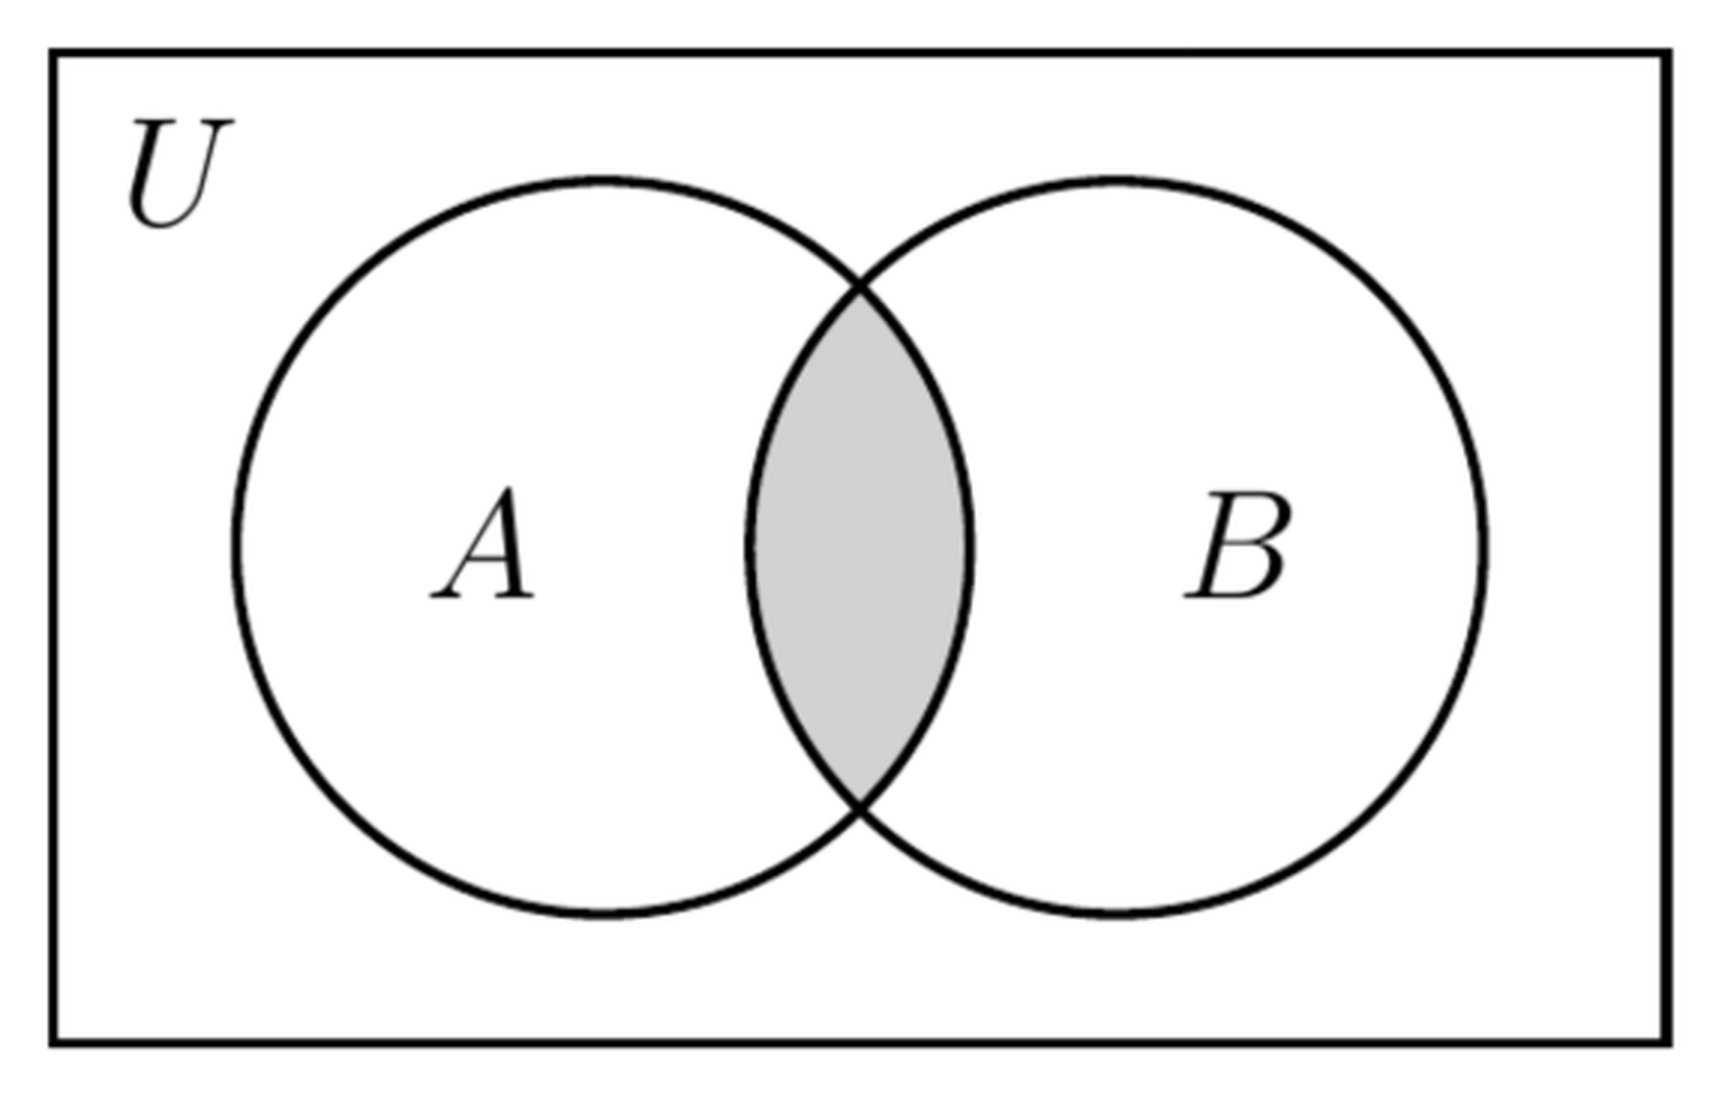
\includegraphics[width=0.38\textwidth]{figures/gao141_q5.png}
\end{center}

\ifanswer
\solbegin
\step{阴影部分表示 $A\cap B=\{4,7\}$.}
\solend
\fi

\item 方程 $2^{\log_3 x}=\dfrac12$ 的解集为\blankline[4.4em].

\ifanswer
\solbegin
\step{$2^{\log_3 x}=2^{-1}\Leftrightarrow\log_3 x=-1\Leftrightarrow x=\dfrac13$，解集为 $\left\{\dfrac13\right\}$.}
\solend
\fi

\item 若集合 $A=\left\{x\mid x^2+ax+\dfrac14=0\right\}$ 有且仅有两个子集，则实数 $a$ 的值为\blankline[4.4em].

\ifanswer
\solbegin
\step{$A$ 有且仅有两个子集，说明 $A$ 恰有一个元素，即方程有两个相等的实数根.}
\step{$\Delta=a^2-4\cdot\dfrac14=0\Rightarrow a=\pm1$.}% 判别式原卷印等腰偏高的高三角 $\Delta$，照录
\solend
\fi

\item 已知关于 $x$ 的方程 $x^2+mx+2m=0$ 的两个实数根分别为 $\alpha$、$\beta$，若 $\alpha^2+\beta^2=5$，则实数 $m=$\blankline[4.4em].

\ifanswer
\solbegin
\step{方程 $x^2+mx+2m=0$ 的两个实数根为 $\alpha$、$\beta$，}
\step{由根与系数的关系得 $\begin{cases}\alpha+\beta=-m\\\alpha\beta=2m\end{cases}$，又因为 $\alpha^2+\beta^2=5$，}
\step{所以 $\alpha^2+\beta^2=(\alpha+\beta)^2-2\alpha\beta=m^2-4m=5$，整理得 $m^2-4m-5=0$，}
\step{解得 $m=5$ 或 $m=-1$，}
\step{当 $m=5$ 时，$\triangle=25-40=-15<0$，无实根，舍去；}% 判别式原卷印扁等边三角 $\triangle$，照录
\step{当 $m=-1$ 时，$\triangle=1+8=9>0$，符合题意，}
\step{所以实数 $m=-1$.}
\solend
\fi

\item 若不等式 $\lvert x-3\rvert+\lvert x-5\rvert\geqslant a$ 对任意的实数 $x$ 恒成立，则实数 $a$ 的取值范围为\blankline[4.4em].

\ifanswer
\solbegin
\step{由三角不等式得 $\lvert x-3\rvert+\lvert x-5\rvert\geqslant\lvert x-3-x+5\rvert=2$，则 $a\leqslant2$.}
\solend
\fi

\item 设集合 $A=\{-3,2\}$，集合 $B=\{x\mid mx+1=0\}$，若 $A\cup B=A$，则实数 $m$ 的值为\blankline[4.4em].

\ifanswer
\solbegin
\step{由 $A\cup B=A$，得 $B\subseteq A$，}% 子集符号原卷印带下划线的 $\subseteq$，照录
\step{当 $m=0$ 时，$B=\varnothing$，满足题意，}
\step{当 $m\neq0$ 时，$B=\left\{-\dfrac1m\right\}$，所以 $-\dfrac1m=2$ 或 $-\dfrac1m=-3$，所以 $m=-\dfrac12$ 或 $m=\dfrac13$，}
\step{综上所述，$m=0$ 或 $m=-\dfrac12$ 或 $m=\dfrac13$.}
\solend
\fi

\item 已知 $m$ 为实数，代数式 $M=\sqrt{m-1}+\sqrt{3-m}$ 的取值范围为\blankline[4.4em].

\ifanswer
\solbegin
\step{根式有意义要求 $m\in[1,3]$，}
\step{此时 $(m-1)(3-m)=1-(m-2)^2$ 的取值范围为 $[0,1]$.}
\step{$M^2=2+2\sqrt{(m-1)(3-m)}$ 的取值范围为 $[2,4]$，又 $M>0$，}
\step{所以 $M\in[\sqrt2,2]$.}
\solend
\fi

\item 设有限集 $M$ 所含元素的个数用 $\mathbf{card}(M)$ 表示，并规定 $\mathbf{card}(\varnothing)=0$. 已知集合 $A,B$ 满足 $A\cup B=\{1,2,3\}$，$A\cap B=\varnothing$，若 $\mathbf{card}(A)\notin A$，$\mathbf{card}(B)\notin B$，则满足条件的所有不同集合 $A$ 的个数为\blankline[4.4em].

\ifanswer
\solbegin
\step{当 $\mathbf{card}(A)=0$ 或 $3$ 时，$A,B$ 中有一个为 $\{1,2,3\}$，不符合条件.}
\step{当 $\mathbf{card}(A)=1$ 时，$\mathbf{card}(B)=2\notin B$，所以 $A=\{2\}$，符合条件.}
\step{当 $\mathbf{card}(A)=2$ 时，$2\notin A$，所以 $B=\{2\}$，$A=\{1,3\}$，符合条件.}
\step{满足条件的集合 $A$ 共 $2$ 个.}
\solend
\fi

\end{enumerate}

\bigsec{二、选择题}

\begin{enumerate}
\setcounter{enumi}{12}

\item “ $x=1$ ” 是 “ $x^2-3x+2=0$ ” 的\mbox{（\quad）}条件.

\keepwithprev
A. 充分非必要\qquad B. 必要非充分

C. 充要\qquad D. 既非充分又非必要

\ifanswer
\solbegin
\step{$x^2-3x+2=0\Leftrightarrow x=1$ 或 $x=2$，所以 “ $x=1$ ” 是其充分非必要条件，}
\step{故选 $A$.}
\solend
\fi

\item 设 $a,b,c\in\R$，则下列命题为真命题的是\mbox{（\quad）}
% 原卷题干只声明 a,b,c，而 A 选项出现未声明的 d，照录（存疑）
\keepwithprev
A. 若 $a>b$ 且 $c>d$，则 $ac>bd$\qquad B. 若 $a^2>b^2$，则 $a>b$

C. 若 $ab>0$ 且 $a>b$，则 $\dfrac1a<\dfrac1b$\qquad D. 若 $a<0<b$，则 $\sqrt{-a}<\sqrt b$

\ifanswer
\solbegin
\step{$ab>0$ 且 $a>b\Rightarrow\dfrac1a-\dfrac1b=\dfrac{b-a}{ab}<0$，所以 $C$ 为真命题，故选 $C$.}
\solend
\fi

\item 已知 $\log_{14}7=a$，$14^b=5$，则 $\log_{35}28=$\mbox{（\quad）}

\keepwithprev
A. $\dfrac{2-a}{2a+b}$\qquad B. $\dfrac{2+a}{a+b}$\qquad C. $\dfrac{2-a}{a+2b}$\qquad D. $\dfrac{2-a}{a+b}$

\ifanswer
\solbegin
\step{$\log_{14}7=a$，$14^b=5$，}
\step{$\log_{35}28=\dfrac{\log_{14}28}{\log_{14}35}=\dfrac{\log_{14}14^2-\log_{14}7}{\log_{14}7+\log_{14}5}=\dfrac{2-a}{a+b}$. 故选 $D$.}
\solend
\fi

\item 关于 $x$ 的不等式 $ax^2+bx+3>0$ 的解集有下列说法，其中正确的个数是\mbox{（\quad）}

\keepwithprev
① 不等式 $ax^2+bx+3>0$ 的解集可以是 $\R$

② 不等式 $ax^2+bx+3>0$ 的解集可以是 $\{x\mid x>3\}$

③ 不等式 $ax^2+bx+3>0$ 的解集可以是 $\varnothing$

④ 不等式 $ax^2+bx+3>0$ 的解集可以是 $\{x\mid -1<x<3\}$

\keepwithprev
A. 4\qquad B. 3\qquad C. 2\qquad D. 1

\ifanswer
\solbegin
\step{$x=0$ 时左端为 $3>0$，解集必含 $0$，所以②③错误.}
\step{①取 $a=1,b=0$，$x^2+3>0$ 的解集为 $\R$，正确.}
\step{④取 $a=-1,b=2$，$-x^2+2x+3=-(x+1)(x-3)>0\Leftrightarrow-1<x<3$，正确.}
\step{正确的有①④，共 $2$ 个，故选 $C$.}
\solend
\fi

\end{enumerate}

\bigsec{三、解答题}

\begin{enumerate}
\setcounter{enumi}{16}

\item 已知集合 $A=\left\{x\mid\dfrac{x-2}{x+3}\geqslant0\right\}$，集合 $B=\{x\mid\lvert x+1\rvert+\lvert x-1\rvert<5\}$，全集 $U=\R$.

(1) 求 $A,B$；

(2) 求 $A\cup B$、$\overline{A\cap B}$.

\ifanswer
\solbegin
\step{(1) 分母不为零，且分子、分母同号或分子为零，}
\step{所以 $\dfrac{x-2}{x+3}\geqslant0\Leftrightarrow x<-3$ 或 $x\geqslant2$，因此 $A=(-\infty,-3)\cup[2,+\infty)$.}
\step{又 $\lvert x+1\rvert+\lvert x-1\rvert=\begin{cases}-2x,&x<-1\\2,&-1\leqslant x\leqslant1\\2x,&x>1\end{cases}$，}
\step{分别解得 $-\dfrac52<x<-1$、$-1\leqslant x\leqslant1$、$1<x<\dfrac52$，因此 $B=\left(-\dfrac52,\dfrac52\right)$.}
\step{(2) 合并两集合所对应的区间，得 $A\cup B=(-\infty,-3)\cup\left(-\dfrac52,+\infty\right)$，}
\step{两集合的公共部分为 $A\cap B=\left[2,\dfrac52\right)$，所以 $\overline{A\cap B}=(-\infty,2)\cup\left[\dfrac52,+\infty\right)$.}
\solend
\fi

\item (1) 已知 $a>b>0$，比较代数式 $\dfrac ab$ 与 $\dfrac{a+1}{b+1}$ 的大小并说明理由；

(2) 已知 $x,y,z$ 都是正实数，$a=x+\dfrac1y,b=y+\dfrac1z,c=z+\dfrac1x$，试用反证法证明 $a,b,c$ 至少有一个不小于 $2$.

\ifanswer
\solbegin
\step{(1) $\dfrac ab-\dfrac{a+1}{b+1}=\dfrac{a(b+1)-b(a+1)}{b(b+1)}=\dfrac{a-b}{b(b+1)}$，}
\step{因为 $a>b>0$，所以 $a-b>0$，$b(b+1)>0$，所以 $\dfrac ab-\dfrac{a+1}{b+1}>0$，}
\step{故 $\dfrac ab>\dfrac{a+1}{b+1}$.}
\step{(2) 假设 $a$、$b$、$c$ 三数都小于 $2$，则 $x+\dfrac1y+y+\dfrac1z+z+\dfrac1x<6$.}
\step{因为 $x,y,z$ 均大于 $0$，}
\step{所以 $x+\dfrac1y+y+\dfrac1z+z+\dfrac1x=x+\dfrac1x+y+\dfrac1y+z+\dfrac1z\geqslant2+2+2=6$，矛盾，}
\step{所以 $a$、$b$、$c$ 三数中至少有一个不小于 $2$.}
\solend
\fi

% 第 19 题长方体无盖贮水池砖墙示意图（题目配图，三版都出）：取原卷 06 页截图去粉色水印、LANCZOS 放大 3 倍
\needvspace{6cm}
\item 如图所示，某工厂要建造一个长方体形无盖贮水池，其容积为 $3200m^3$，深为 $2m$.

(1) 若水池的长比宽至少多 $60m$，求水池的宽的最大值；

(2) 若池底每平方米的造价为 $150$ 元，池壁每平方米的造价为 $120$ 元，那么怎样设计水池的长和宽能使总造价最低？最低总造价是多少？

\begin{center}
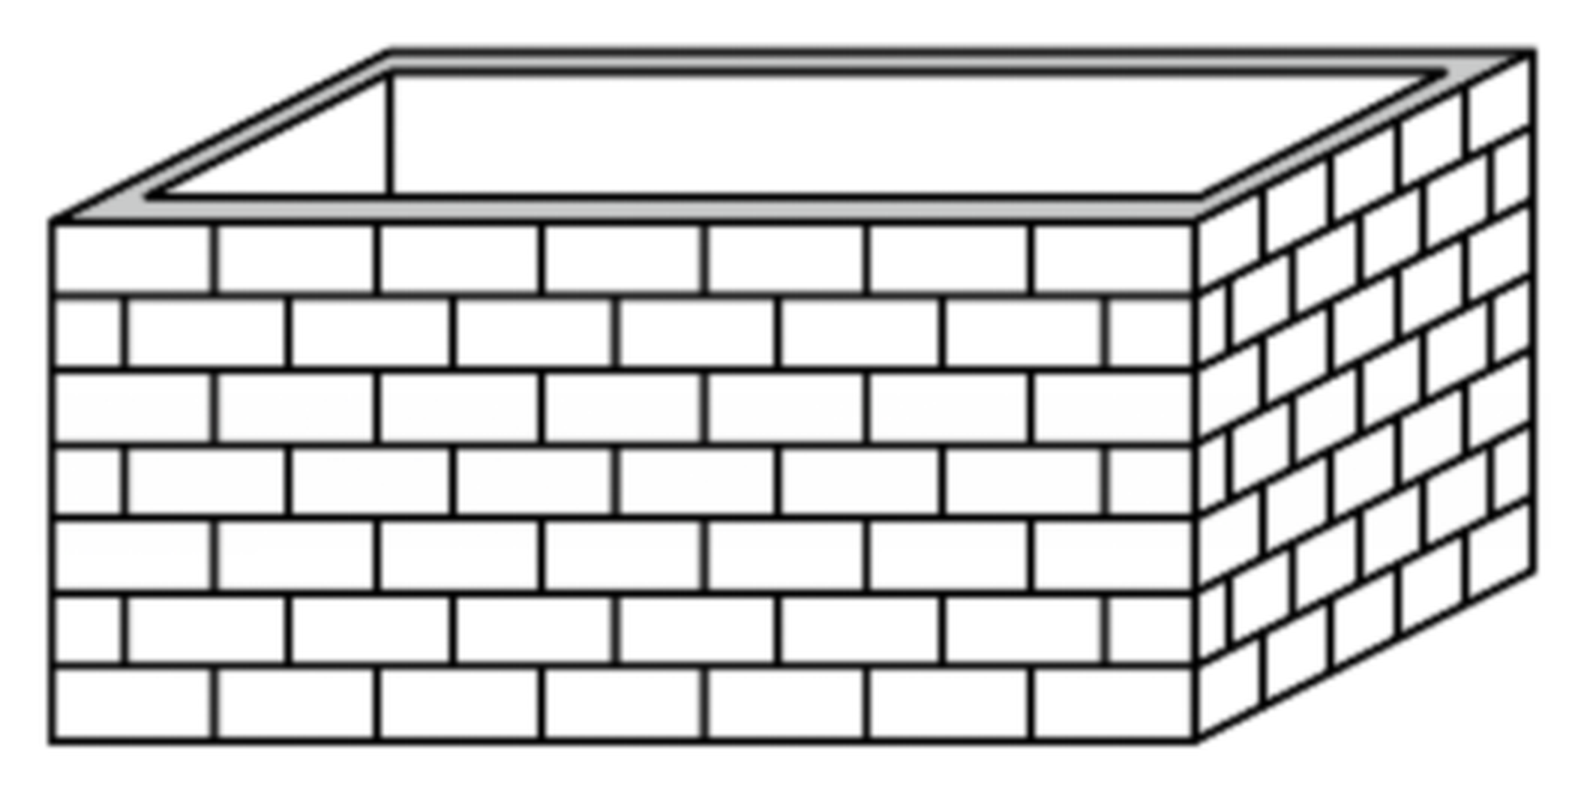
\includegraphics[width=0.42\textwidth]{figures/gao141_q19.png}
\end{center}

\ifanswer
\solbegin
\step{(1) 设水池的长、宽分别为 $xm$，$ym$，则 $x-y\geqslant60$，且 $x$、$y>0$，}
\step{由题意得 $2xy=3200$，即 $x=\dfrac{1600}{y}$，所以 $\dfrac{1600}{y}-y\geqslant60$，}
\step{因为 $y>0$，所以 $1600-y^2\geqslant60y$，}
\step{即 $y^2+60y-1600=(y+80)(y-20)\leqslant0$，解得 $-80\leqslant y\leqslant20$，}
\step{又 $y>0$，所以 $0<y\leqslant20$，所以水池的宽的最大值为 $20m$.}
\step{(2) 设水池总造价为 $z$ 元，}
\step{则 $z=1600\times150+2\times(2x+2y)\times120=240000+480(x+y)$，}
\step{又因为 $y=\dfrac{1600}{x}$，}
\step{所以 $z=240000+\left(x+\dfrac{1600}{x}\right)\times480\geqslant240000+480\times2\sqrt{1600}$}
\step{$=240000+38400=278400$，}
\step{当且仅当 $x=\dfrac{1600}{x}$，即 $x=y=40$ 时取等号，}
\step{所以，将水池的池底设计为边长为 $40m$ 的正方形时总造价最低，}
\step{最低总造价为 $278400$ 元.}
\solend
\fi

\item 已知 $a\in\R$，设集合 $A=\{x\mid ax^2-3x+2<ax-1\}$.

(1) 若 $A=(1,3)$，求实数 $a$ 的值；

(2) 当 $a>0$ 时，求 $A$；

(3) 若 “ $x\in\left(\dfrac12,+\infty\right)$ ” 是 “ $x\in A$ ” 的必要非充分条件，求实数 $a$ 的取值范围.

\ifanswer
\solbegin
\step{原不等式等价于 $ax^2-(a+3)x+3<0\Leftrightarrow(x-1)(ax-3)<0$，}
\step{(1) $A=(1,3)$ 为有界区间，因此 $a>0$，两根为 $1$ 和 $\dfrac3a$，于是 $\dfrac3a=3$，得 $a=1$；}
\step{此时 $(x-1)(x-3)<0$ 的解集确为 $(1,3)$.}
\step{(2) 当 $a>0$ 时，二次项系数为正，比较 $1$ 与 $\dfrac3a$，得 $A=\begin{cases}\left(1,\dfrac3a\right),&0<a<3\\\varnothing,&a=3\\\left(\dfrac3a,1\right),&a>3\end{cases}$，}
\step{其中 $a=3$ 时，原不等式为 $3(x-1)^2<0$，无解.}
\step{(3) 记 $S=\left(\dfrac12,+\infty\right)$，题意要求 $A\subset S$.}% 子集符号原卷印单线 $\subset$，照录
\step{由于对任意 $a$ 都有 $1\notin A$，而 $1\in S$，所以只需满足 $A\subseteq S$.}
\step{当 $a<0$ 时，$A=\left(-\infty,\dfrac3a\right)\cup(1,+\infty)$，含有小于 $\dfrac12$ 的数，不符合条件.}
\step{当 $a=0$ 时，$A=(1,+\infty)$，符合条件.}
\step{当 $0<a<3$ 时，$A=\left(1,\dfrac3a\right)\subseteq S$；}
\step{当 $a=3$ 时，$A=\varnothing\subseteq S$，均符合条件；}
\step{当 $a>3$ 时，$A=\left(\dfrac3a,1\right)$，所以 $A\subseteq S\Leftrightarrow\dfrac3a\geqslant\dfrac12\Leftrightarrow a\leqslant6$；}
\step{因此实数 $a$ 的取值范围为 $[0,6]$.}
\solend
\fi

\item 甲、乙两同学探讨了一个问题：已知正实数 $x,y$ 满足 $3x+y=1$，求 $\dfrac1x+\dfrac1y$ 的最小值.

甲给出的解法：由 $1=3x+y\geqslant2\sqrt{3xy}$，得 $\sqrt{xy}\leqslant\dfrac{\sqrt3}{6}$，所以 $\dfrac1x+\dfrac1y\geqslant2\sqrt{\dfrac1{xy}}\geqslant4\sqrt3$. 因此 $\dfrac1x+\dfrac1y$ 的最小值为 $4\sqrt3$.

乙给出的解法：$\dfrac1x+\dfrac1y=\left(\dfrac1x+\dfrac1y\right)(3x+y)=4+\dfrac yx+\dfrac{3x}{y}$，因为 $x,y$ 均为正实数，所以 $\dfrac1x+\dfrac1y\geqslant4+2\sqrt{\dfrac yx\cdot\dfrac{3x}{y}}=4+2\sqrt3$.

(1) 请判断上述哪位同学的解法正确，哪位同学的解法错误，并指出错误的原因；

(2) 结合上述探讨，试求当 $0<x<\dfrac12$ 时，$\dfrac1x+\dfrac1{1-2x}$ 的最小值以及此时实数 $x$ 的值；

(3) 已知 $x$ 为正实数，$y$ 为非负实数，且 $x+2y=2$，求 $\dfrac{x^2+1}{x}+\dfrac{2y^2}{y+1}$ 的最小值以及此时实数 $x,y$ 的值.

\ifanswer
\solbegin
\step{(1) 甲的推导中，$3x+y\geqslant2\sqrt{3xy}$ 取等号要求 $3x=y$，}
\step{$\dfrac1x+\dfrac1y\geqslant\dfrac2{\sqrt{xy}}$ 取等号要求 $x=y$，两者对正实数 $x,y$ 不能同时成立，}
\step{因此不能将 $4\sqrt3$ 判为最小值，甲错误.}
\step{乙的等号条件为 $\dfrac yx=\dfrac{3x}{y}$，即 $y=\sqrt3 x$；}
\step{结合 $3x+y=1$，得 $x=\dfrac1{3+\sqrt3},y=\dfrac{\sqrt3}{3+\sqrt3}$ 均为正数，等号可以成立，}
\step{因此乙正确，最小值为 $4+2\sqrt3$.}
\step{(2) 令 $t=1-2x>0$，则 $2x+t=1$.}
\step{$\dfrac1x+\dfrac1t=\left(\dfrac1x+\dfrac1t\right)(2x+t)=3+\dfrac tx+\dfrac{2x}{t}\geqslant3+2\sqrt2$，}
\step{当且仅当 $\dfrac tx=\dfrac{2x}{t}$，即 $t=\sqrt2 x$ 时取等号，}
\step{由 $2x+t=1$，得 $x=\dfrac1{2+\sqrt2}=\dfrac{2-\sqrt2}{2}\in\left(0,\dfrac12\right)$，}
\step{因此最小值为 $3+2\sqrt2$，此时 $x=\dfrac{2-\sqrt2}{2}$.}
\step{(3) 记目标式为 $F$，利用 $x+2y=2$，}
\step{得 $F=x+\dfrac1x+2y-2+\dfrac2{y+1}=\dfrac1x+\dfrac2{y+1}$，}
\step{又 $x+2(y+1)=4$，且 $x>0$、$y+1>0$，}
\step{所以 $4F=\left(\dfrac1x+\dfrac2{y+1}\right)(x+2(y+1))=5+2\left(\dfrac{y+1}{x}+\dfrac{x}{y+1}\right)$}
\step{$\geqslant5+2\times2=9$，当且仅当 $\dfrac{y+1}{x}=\dfrac{x}{y+1}$，即 $x=y+1$ 时取等号.}
\step{联立 $x+2y=2$，得 $x=\dfrac43$、$y=\dfrac13$，满足题设条件，}
\step{因此最小值为 $\dfrac94$，此时 $x=\dfrac43$，$y=\dfrac13$.}
\solend
\fi

\end{enumerate}

\end{document}
"
% 紧凑版：xelatex "\def\iscompact{1}% 高一141_彭浦中学_期中.tex
%   —— 高一上数学"2026-2027 年彭浦中学高一上期中"（试卷版/答案版/紧凑版）
% 试卷版：xelatex 高一141_彭浦中学_期中.tex
% 答案版：xelatex "\def\isanswer{1}\input{高一141_彭浦中学_期中.tex}"
% 紧凑版：xelatex "\def\iscompact{1}\input{高一141_彭浦中学_期中.tex}"
%
% ① 原始材料：微信公众号"魔都数学加油站"文章，连载"27学年高一141"，原文标题
% "27学年高一141——2026-2027年上海市彭浦中学高一上期中"；
% 原文链接：https://mp.weixin.qq.com/s/V_8bEhC6geeFyQysmtqUtQ。
% 正文为 9 张 PNG 页（01、05、06、07、09 为 2560x3620；02、03、04、08 为 4762x6735，
% 同一篇各页分辨率不同，逐页按各自分辨率放大裁图核对），题目下印【解析】，为讲评版。
% 题目、解析均据原图转录；卷面粉红色水印"魔都数学加油站"及公众号页脚未录入。
% 全卷 2 幅插图，均属题目配图（在 \ifanswer 外、三版都出）、取原卷截图去粉色水印、
% LANCZOS 放大 3 倍：第 5 题韦恩图（01 页，全集 U 矩形内两圆相交、交集阴影、A/B/U 标注）、
% 第 19 题长方体无盖贮水池砖墙示意图（06 页右上）。通读 9 页确认除这 2 幅外无其它
% 插图/表格，亦无"题干写如图而源码漏图"（仅 Q5"图中阴影部分"、Q19"如图所示"两处提到图）。
%
% 卷首标题：原卷印作"2026-2027 年彭浦中学高一上期中"（公众号标题中的"上海市"
% 卷面标题行没有，本稿照卷面），年份区间按全稿惯例排 en dash；原卷未印副标题，
% 本卷为期中卷、跨集合与常用逻辑用语／不等式／函数三章，按题目内容补出
% "集合与常用逻辑用语、不等式、函数"（与 高一140 同期中卷口径相同）：
% 集合与逻辑见 Q5、Q10、Q12、Q13、Q16、Q17、Q20，不等式见 Q4、Q9、Q14、Q18、
% Q19、Q21，函数（指数／对数）见 Q6、Q15。
%
% 题号体例：本卷共 19 题——一、填空题 3—12（10 题）、二、选择题 13—16（4 题）、
% 三、解答题 17—21（5 题）。三节分别 \setcounter{enumi}{2}／{12}／{16}。
% 原卷从第 3 题起、无第 1、2 题，本稿保留原题号；全卷无附加题节。
%
% ② 与原卷的排版差异：
%   ① 原文从第 3 题起，本稿保留原题号；
%   ② 原卷 19 题题下均印【解析】，无独立【答案】段、无"答案印题干括号且无解析"、
%      无"只印【答案】无解析"一型：填空题与解答题的答案落在【解析】末句
%      （Q3—Q12、Q17—Q21），四道选择题答案在【解析】末句"故选 …"
%      （Q13 选 A、Q14 选 C、Q15 选 D、Q16 选 C），题干括号内一律留空；
%      本稿 19 题一律 \solbegin…\solend、全卷不提 \ans{}，答案版【解析】标记数
%      = 19 = 全卷题数（无【答案】标记）；
%   ③ 原卷未印副标题，本稿按"知识模块"口径补出；
%   ④ 原卷填空横线按全稿惯例排 \blankline[4.4em]；选择题括号排 \mbox{（\quad）}，
%      选项段／命题段前按惯例加 \keepwithprev（Q16 两枚：命题列与选项段各一）；
%      解答题不留作答区、不加 \anspace（原卷为讲评版，与 129／131／132／133／136／140 同）；
%   ⑤ 原卷数集混排：黑板粗体 R（Q14 题干、Q16 ① 与解析、Q17 全集、Q20 题干）
%      按全稿惯例统一改 \R；空集记号 \varnothing；绝对值排 \lvert…\rvert，
%      集合描述竖线排 \mid；不等号按全稿惯例排 \leqslant／\geqslant；
%      补集照原卷上划线排 \overline{A\cap B}（Q17(2) 题干与解析）；
%      原卷"card"记号排黑体正体（Q12），本稿照录 \mathbf{card}，未改斜体
%      （与 高一66 同题口径不同：那份原卷 card 排斜体、照录 $card(M)$）；
%   ⑥ 子题标号 (1)(2)(3) 原卷印半角括号，照录；圈数字 ①②③④ 在正文（文本模式）
%      按原卷照录，未进数学式；数学式内半角逗号照录（如 Q12"$A,B$"、"{1,2,3}"、
%      Q14"$a,b,c\in\R$"、Q15"$\log_{14}7=a$，$14^b=5$"、Q16"$a=1,b=0$"、
%      Q18"$x,y,z$"、Q20"$x,y$"、Q21"$x,y$"）；全卷行末西文句点照录为 ASCII 句点；
%      行中全角逗号、顿号照录；
%   ⑦ 题干中的中文弯引号按原卷照录（Q13、Q20(3) 的 “ ” 及引号内空格），
%      注释内一律 ASCII 引号；
%   ⑧ 两幅题目配图各在 \item 之前加 \needvspace 守卫整块推走（Q5 5cm、Q19 6cm），
%      守卫放在 \item 之前而非 \bigsec 之后——两题均非各节首题，不触发 B 类
%      "节标题落页末"（照 高一26／40／59／136／140 成例）；三版切页审计均"合计异常：无"；
%   ⑨ 跨页续印按题合并：Q8 题干与【解析】首行在 01 页、后 6 行在 02 页；
%      Q15 题干在 03 页、【解析】在 04 页；Q17 题干与【解析】前 2 行在 04 页、
%      后 4 行在 05 页；Q19 题干在 05 页末、(1)(2) 小问与砖墙图与【解析】在 06 页；
%      Q20 题干 (1)(2) 在 06 页末、(3) 与【解析】在 07 页；Q21 题干与【解析】
%      前 6 行在 08 页、后 12 行在 09 页；Q16、Q18 全在各自页内；
%      本稿按题连排，不丢行；
%   ⑩ 原卷无红色加粗标签（【解析】均黑色印刷，Q16 解析 "①取…""④取…" 与
%      Q20 解析 "(2)" 等分步标签亦黑色），故本卷未用 \stepm；
%   ⑪ 原卷 Q19 题干把数值与单位（3200m³、2m、60m、150 元、120 元、40m、20m、
%      278400 元）印作略粗的西文字形，本稿按全稿惯例（高一70／72 同类题）排普通
%      数学体，未加粗。
%
% ③ 行数复核：一条 \step = 原卷解析的一个印刷行，cases 块作一个印刷行计。逐题数 \step
%   条数，合计 92 条（Q3：1；Q4：1；Q5：1；Q6：1；Q7：2；Q8：7；Q9：1；Q10：4；
%   Q11：4；Q12：4；Q13：2；Q14：1；Q15：2；Q16：4；Q17：6；Q18：7；Q19：13；
%   Q20：13；Q21：18），与原卷印刷行逐题相等。全卷 19 题均印【解析】、无独立 \ans{}，
%   答案版【解析】标记数 = 19 = 全卷题数。
%
% ④ 判别式／子集符号结论（逐处放大原图照录、不得统一）：
%   判别式：全卷 3 处——第 7 题【解析】"$\Delta=a^2-4\cdot\frac14=0$"一处原卷印
%     等腰、偏高的高三角 $\Delta$，照录 \Delta；第 8 题【解析】
%     "$\triangle=25-40=-15<0$"与"$\triangle=1+8=9>0$"两处原卷印扁等边三角
%     $\triangle$，照录 \triangle。两形不同，逐处照录未统一。
%   子集：全卷 6 处——第 10 题【解析】"$B\subseteq A$"一处、第 20 题【解析】
%     "所以只需满足 $A\subseteq S$"、"$A=\left(1,\frac3a\right)\subseteq S$"、
%     "$A=\varnothing\subseteq S$"、"$A\subseteq S\Leftrightarrow\frac3a\geqslant\frac12$"
%     四处，共 5 处原卷印带下划线的 $\subseteq$，照录 \subseteq；第 20 题【解析】
%     (3) 首行"题意要求 $A\subset S$"一处原卷印单线 $\subset$，照录 \subset
%     （下行因 $1\in S$ 而 $1\notin A$，改述为 $A\subseteq S$，两者逻辑一致、非笔误）。
%
% ⑤ 存疑照录（照录未改，正文对应处另有 % 注）：
%   第 14 题题干"设 $a,b,c\in\R$"只声明 $a,b,c$，而 A 选项"若 $a>b$ 且 $c>d$，
%     则 $ac>bd$"引入未声明的 $d$，原卷变量声明与选项不统一，照录未补。
%   全卷除此 1 条外未发现其它笔误／自相矛盾处。
%
% ⑥ 跨页续印按题合并说明：见 ② ⑨。
%
\documentclass[a4paper,11pt]{article}
\usepackage{common}

\begin{document}

\examtitlest[3]{2026--2027 年彭浦中学高一上期中}{集合与常用逻辑用语、不等式、函数}

\bigsec{一、填空题}

\begin{enumerate}
\setcounter{enumi}{2}

\item 已知 $m$ 为实数，若 $1\in\{m,m^2\}$，则 $m$ 的值为\blankline[4.4em].

\ifanswer
\solbegin
\step{$m=1$ 或 $m^2=1$，得 $m=\pm1$；按列举项互异口径排除 $m=m^2=1$，得 $m=-1$.}
\solend
\fi

\item 已知 $2<a<4$，$-2<b<1$，则 $2a+b$ 的取值范围为\blankline[4.4em].

\ifanswer
\solbegin
\step{$4<2a<8$，与 $-2<b<1$ 相加，得 $2<2a+b<9$，取值范围为 $(2,9)$.}
\solend
\fi

% 第 5 题韦恩图（题目配图，三版都出）：取原卷 01 页截图去粉色水印、LANCZOS 放大 3 倍
\needvspace{5cm}
\item 已知集合 $A=\{-1,-2,1,4,7\}$，$B=\{x\mid x>1\}$，用列举法表示图中阴影部分所表示的集合为\blankline[4.4em].

\begin{center}
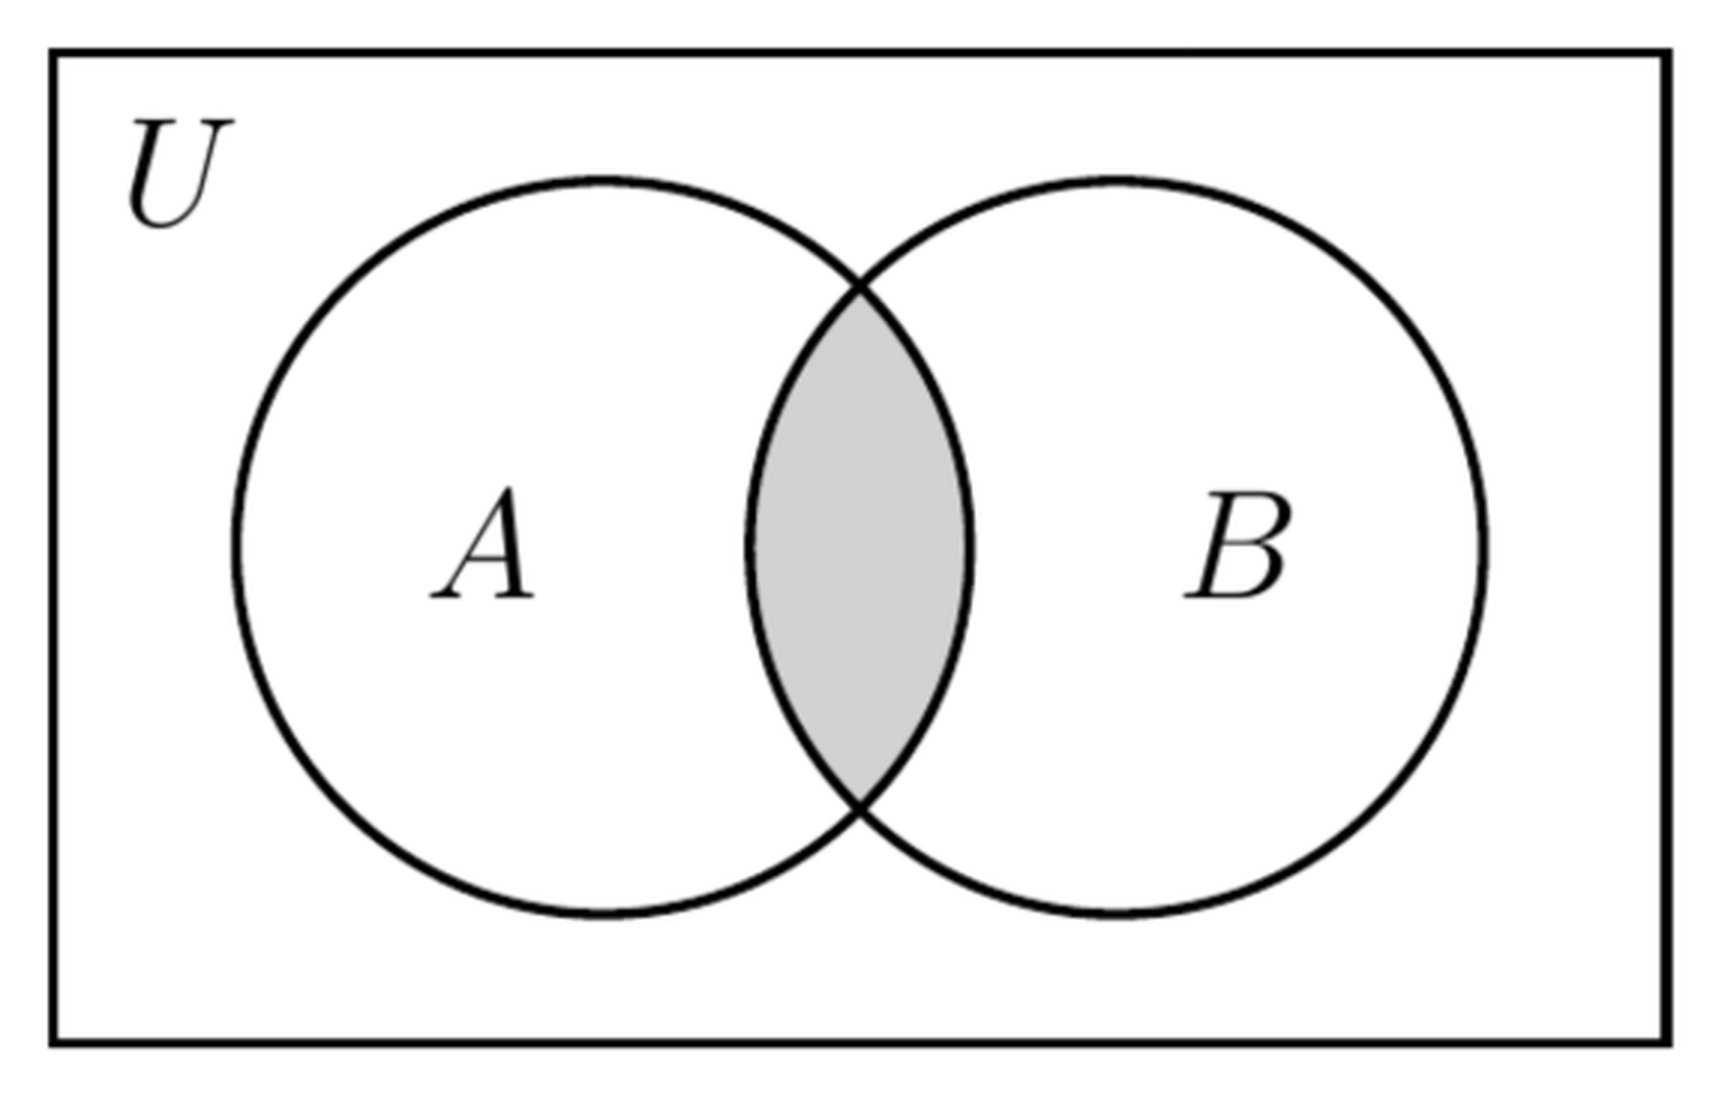
\includegraphics[width=0.38\textwidth]{figures/gao141_q5.png}
\end{center}

\ifanswer
\solbegin
\step{阴影部分表示 $A\cap B=\{4,7\}$.}
\solend
\fi

\item 方程 $2^{\log_3 x}=\dfrac12$ 的解集为\blankline[4.4em].

\ifanswer
\solbegin
\step{$2^{\log_3 x}=2^{-1}\Leftrightarrow\log_3 x=-1\Leftrightarrow x=\dfrac13$，解集为 $\left\{\dfrac13\right\}$.}
\solend
\fi

\item 若集合 $A=\left\{x\mid x^2+ax+\dfrac14=0\right\}$ 有且仅有两个子集，则实数 $a$ 的值为\blankline[4.4em].

\ifanswer
\solbegin
\step{$A$ 有且仅有两个子集，说明 $A$ 恰有一个元素，即方程有两个相等的实数根.}
\step{$\Delta=a^2-4\cdot\dfrac14=0\Rightarrow a=\pm1$.}% 判别式原卷印等腰偏高的高三角 $\Delta$，照录
\solend
\fi

\item 已知关于 $x$ 的方程 $x^2+mx+2m=0$ 的两个实数根分别为 $\alpha$、$\beta$，若 $\alpha^2+\beta^2=5$，则实数 $m=$\blankline[4.4em].

\ifanswer
\solbegin
\step{方程 $x^2+mx+2m=0$ 的两个实数根为 $\alpha$、$\beta$，}
\step{由根与系数的关系得 $\begin{cases}\alpha+\beta=-m\\\alpha\beta=2m\end{cases}$，又因为 $\alpha^2+\beta^2=5$，}
\step{所以 $\alpha^2+\beta^2=(\alpha+\beta)^2-2\alpha\beta=m^2-4m=5$，整理得 $m^2-4m-5=0$，}
\step{解得 $m=5$ 或 $m=-1$，}
\step{当 $m=5$ 时，$\triangle=25-40=-15<0$，无实根，舍去；}% 判别式原卷印扁等边三角 $\triangle$，照录
\step{当 $m=-1$ 时，$\triangle=1+8=9>0$，符合题意，}
\step{所以实数 $m=-1$.}
\solend
\fi

\item 若不等式 $\lvert x-3\rvert+\lvert x-5\rvert\geqslant a$ 对任意的实数 $x$ 恒成立，则实数 $a$ 的取值范围为\blankline[4.4em].

\ifanswer
\solbegin
\step{由三角不等式得 $\lvert x-3\rvert+\lvert x-5\rvert\geqslant\lvert x-3-x+5\rvert=2$，则 $a\leqslant2$.}
\solend
\fi

\item 设集合 $A=\{-3,2\}$，集合 $B=\{x\mid mx+1=0\}$，若 $A\cup B=A$，则实数 $m$ 的值为\blankline[4.4em].

\ifanswer
\solbegin
\step{由 $A\cup B=A$，得 $B\subseteq A$，}% 子集符号原卷印带下划线的 $\subseteq$，照录
\step{当 $m=0$ 时，$B=\varnothing$，满足题意，}
\step{当 $m\neq0$ 时，$B=\left\{-\dfrac1m\right\}$，所以 $-\dfrac1m=2$ 或 $-\dfrac1m=-3$，所以 $m=-\dfrac12$ 或 $m=\dfrac13$，}
\step{综上所述，$m=0$ 或 $m=-\dfrac12$ 或 $m=\dfrac13$.}
\solend
\fi

\item 已知 $m$ 为实数，代数式 $M=\sqrt{m-1}+\sqrt{3-m}$ 的取值范围为\blankline[4.4em].

\ifanswer
\solbegin
\step{根式有意义要求 $m\in[1,3]$，}
\step{此时 $(m-1)(3-m)=1-(m-2)^2$ 的取值范围为 $[0,1]$.}
\step{$M^2=2+2\sqrt{(m-1)(3-m)}$ 的取值范围为 $[2,4]$，又 $M>0$，}
\step{所以 $M\in[\sqrt2,2]$.}
\solend
\fi

\item 设有限集 $M$ 所含元素的个数用 $\mathbf{card}(M)$ 表示，并规定 $\mathbf{card}(\varnothing)=0$. 已知集合 $A,B$ 满足 $A\cup B=\{1,2,3\}$，$A\cap B=\varnothing$，若 $\mathbf{card}(A)\notin A$，$\mathbf{card}(B)\notin B$，则满足条件的所有不同集合 $A$ 的个数为\blankline[4.4em].

\ifanswer
\solbegin
\step{当 $\mathbf{card}(A)=0$ 或 $3$ 时，$A,B$ 中有一个为 $\{1,2,3\}$，不符合条件.}
\step{当 $\mathbf{card}(A)=1$ 时，$\mathbf{card}(B)=2\notin B$，所以 $A=\{2\}$，符合条件.}
\step{当 $\mathbf{card}(A)=2$ 时，$2\notin A$，所以 $B=\{2\}$，$A=\{1,3\}$，符合条件.}
\step{满足条件的集合 $A$ 共 $2$ 个.}
\solend
\fi

\end{enumerate}

\bigsec{二、选择题}

\begin{enumerate}
\setcounter{enumi}{12}

\item “ $x=1$ ” 是 “ $x^2-3x+2=0$ ” 的\mbox{（\quad）}条件.

\keepwithprev
A. 充分非必要\qquad B. 必要非充分

C. 充要\qquad D. 既非充分又非必要

\ifanswer
\solbegin
\step{$x^2-3x+2=0\Leftrightarrow x=1$ 或 $x=2$，所以 “ $x=1$ ” 是其充分非必要条件，}
\step{故选 $A$.}
\solend
\fi

\item 设 $a,b,c\in\R$，则下列命题为真命题的是\mbox{（\quad）}
% 原卷题干只声明 a,b,c，而 A 选项出现未声明的 d，照录（存疑）
\keepwithprev
A. 若 $a>b$ 且 $c>d$，则 $ac>bd$\qquad B. 若 $a^2>b^2$，则 $a>b$

C. 若 $ab>0$ 且 $a>b$，则 $\dfrac1a<\dfrac1b$\qquad D. 若 $a<0<b$，则 $\sqrt{-a}<\sqrt b$

\ifanswer
\solbegin
\step{$ab>0$ 且 $a>b\Rightarrow\dfrac1a-\dfrac1b=\dfrac{b-a}{ab}<0$，所以 $C$ 为真命题，故选 $C$.}
\solend
\fi

\item 已知 $\log_{14}7=a$，$14^b=5$，则 $\log_{35}28=$\mbox{（\quad）}

\keepwithprev
A. $\dfrac{2-a}{2a+b}$\qquad B. $\dfrac{2+a}{a+b}$\qquad C. $\dfrac{2-a}{a+2b}$\qquad D. $\dfrac{2-a}{a+b}$

\ifanswer
\solbegin
\step{$\log_{14}7=a$，$14^b=5$，}
\step{$\log_{35}28=\dfrac{\log_{14}28}{\log_{14}35}=\dfrac{\log_{14}14^2-\log_{14}7}{\log_{14}7+\log_{14}5}=\dfrac{2-a}{a+b}$. 故选 $D$.}
\solend
\fi

\item 关于 $x$ 的不等式 $ax^2+bx+3>0$ 的解集有下列说法，其中正确的个数是\mbox{（\quad）}

\keepwithprev
① 不等式 $ax^2+bx+3>0$ 的解集可以是 $\R$

② 不等式 $ax^2+bx+3>0$ 的解集可以是 $\{x\mid x>3\}$

③ 不等式 $ax^2+bx+3>0$ 的解集可以是 $\varnothing$

④ 不等式 $ax^2+bx+3>0$ 的解集可以是 $\{x\mid -1<x<3\}$

\keepwithprev
A. 4\qquad B. 3\qquad C. 2\qquad D. 1

\ifanswer
\solbegin
\step{$x=0$ 时左端为 $3>0$，解集必含 $0$，所以②③错误.}
\step{①取 $a=1,b=0$，$x^2+3>0$ 的解集为 $\R$，正确.}
\step{④取 $a=-1,b=2$，$-x^2+2x+3=-(x+1)(x-3)>0\Leftrightarrow-1<x<3$，正确.}
\step{正确的有①④，共 $2$ 个，故选 $C$.}
\solend
\fi

\end{enumerate}

\bigsec{三、解答题}

\begin{enumerate}
\setcounter{enumi}{16}

\item 已知集合 $A=\left\{x\mid\dfrac{x-2}{x+3}\geqslant0\right\}$，集合 $B=\{x\mid\lvert x+1\rvert+\lvert x-1\rvert<5\}$，全集 $U=\R$.

(1) 求 $A,B$；

(2) 求 $A\cup B$、$\overline{A\cap B}$.

\ifanswer
\solbegin
\step{(1) 分母不为零，且分子、分母同号或分子为零，}
\step{所以 $\dfrac{x-2}{x+3}\geqslant0\Leftrightarrow x<-3$ 或 $x\geqslant2$，因此 $A=(-\infty,-3)\cup[2,+\infty)$.}
\step{又 $\lvert x+1\rvert+\lvert x-1\rvert=\begin{cases}-2x,&x<-1\\2,&-1\leqslant x\leqslant1\\2x,&x>1\end{cases}$，}
\step{分别解得 $-\dfrac52<x<-1$、$-1\leqslant x\leqslant1$、$1<x<\dfrac52$，因此 $B=\left(-\dfrac52,\dfrac52\right)$.}
\step{(2) 合并两集合所对应的区间，得 $A\cup B=(-\infty,-3)\cup\left(-\dfrac52,+\infty\right)$，}
\step{两集合的公共部分为 $A\cap B=\left[2,\dfrac52\right)$，所以 $\overline{A\cap B}=(-\infty,2)\cup\left[\dfrac52,+\infty\right)$.}
\solend
\fi

\item (1) 已知 $a>b>0$，比较代数式 $\dfrac ab$ 与 $\dfrac{a+1}{b+1}$ 的大小并说明理由；

(2) 已知 $x,y,z$ 都是正实数，$a=x+\dfrac1y,b=y+\dfrac1z,c=z+\dfrac1x$，试用反证法证明 $a,b,c$ 至少有一个不小于 $2$.

\ifanswer
\solbegin
\step{(1) $\dfrac ab-\dfrac{a+1}{b+1}=\dfrac{a(b+1)-b(a+1)}{b(b+1)}=\dfrac{a-b}{b(b+1)}$，}
\step{因为 $a>b>0$，所以 $a-b>0$，$b(b+1)>0$，所以 $\dfrac ab-\dfrac{a+1}{b+1}>0$，}
\step{故 $\dfrac ab>\dfrac{a+1}{b+1}$.}
\step{(2) 假设 $a$、$b$、$c$ 三数都小于 $2$，则 $x+\dfrac1y+y+\dfrac1z+z+\dfrac1x<6$.}
\step{因为 $x,y,z$ 均大于 $0$，}
\step{所以 $x+\dfrac1y+y+\dfrac1z+z+\dfrac1x=x+\dfrac1x+y+\dfrac1y+z+\dfrac1z\geqslant2+2+2=6$，矛盾，}
\step{所以 $a$、$b$、$c$ 三数中至少有一个不小于 $2$.}
\solend
\fi

% 第 19 题长方体无盖贮水池砖墙示意图（题目配图，三版都出）：取原卷 06 页截图去粉色水印、LANCZOS 放大 3 倍
\needvspace{6cm}
\item 如图所示，某工厂要建造一个长方体形无盖贮水池，其容积为 $3200m^3$，深为 $2m$.

(1) 若水池的长比宽至少多 $60m$，求水池的宽的最大值；

(2) 若池底每平方米的造价为 $150$ 元，池壁每平方米的造价为 $120$ 元，那么怎样设计水池的长和宽能使总造价最低？最低总造价是多少？

\begin{center}
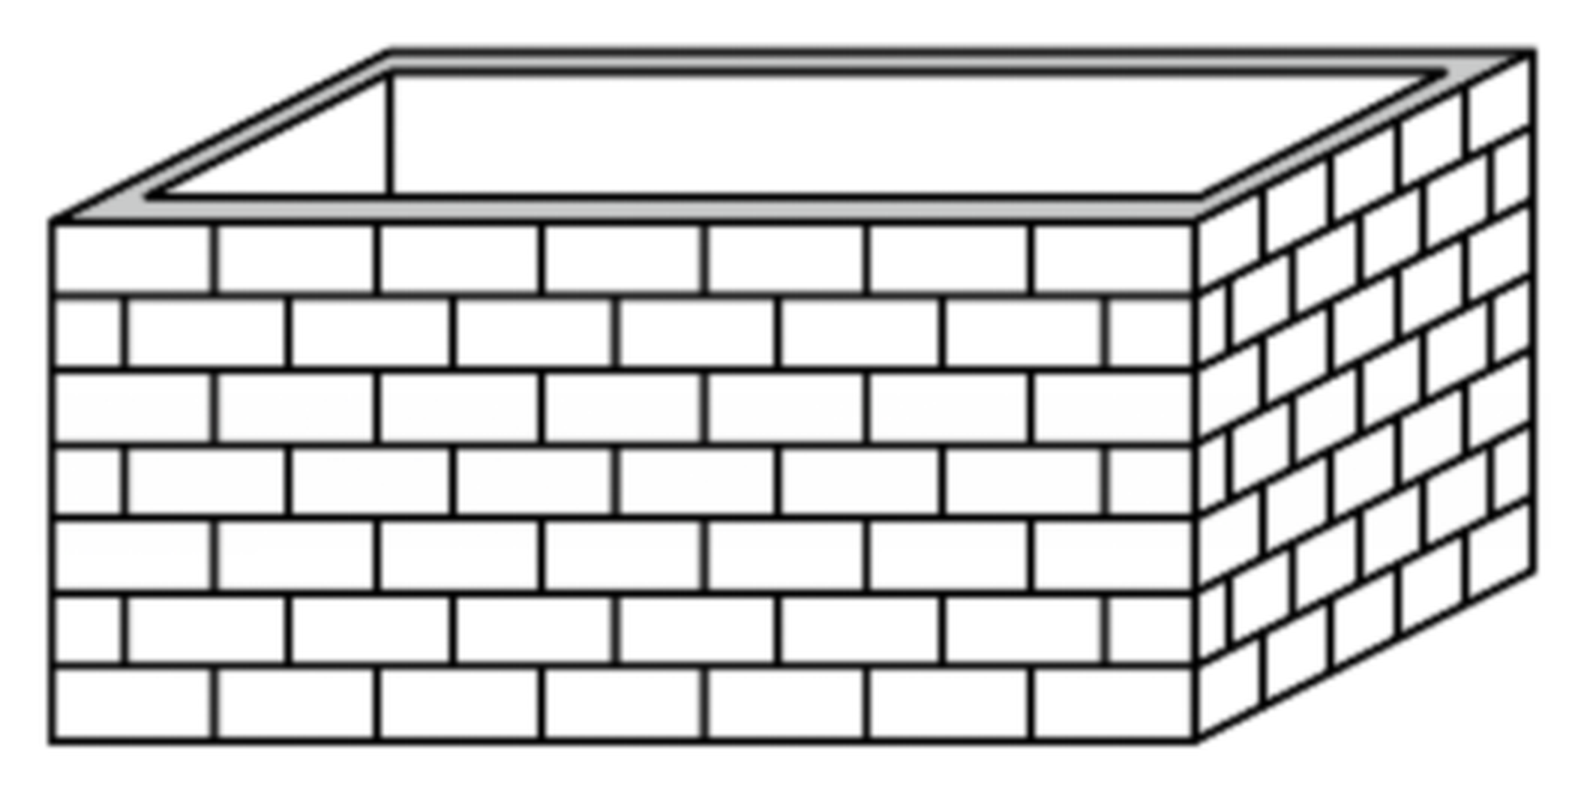
\includegraphics[width=0.42\textwidth]{figures/gao141_q19.png}
\end{center}

\ifanswer
\solbegin
\step{(1) 设水池的长、宽分别为 $xm$，$ym$，则 $x-y\geqslant60$，且 $x$、$y>0$，}
\step{由题意得 $2xy=3200$，即 $x=\dfrac{1600}{y}$，所以 $\dfrac{1600}{y}-y\geqslant60$，}
\step{因为 $y>0$，所以 $1600-y^2\geqslant60y$，}
\step{即 $y^2+60y-1600=(y+80)(y-20)\leqslant0$，解得 $-80\leqslant y\leqslant20$，}
\step{又 $y>0$，所以 $0<y\leqslant20$，所以水池的宽的最大值为 $20m$.}
\step{(2) 设水池总造价为 $z$ 元，}
\step{则 $z=1600\times150+2\times(2x+2y)\times120=240000+480(x+y)$，}
\step{又因为 $y=\dfrac{1600}{x}$，}
\step{所以 $z=240000+\left(x+\dfrac{1600}{x}\right)\times480\geqslant240000+480\times2\sqrt{1600}$}
\step{$=240000+38400=278400$，}
\step{当且仅当 $x=\dfrac{1600}{x}$，即 $x=y=40$ 时取等号，}
\step{所以，将水池的池底设计为边长为 $40m$ 的正方形时总造价最低，}
\step{最低总造价为 $278400$ 元.}
\solend
\fi

\item 已知 $a\in\R$，设集合 $A=\{x\mid ax^2-3x+2<ax-1\}$.

(1) 若 $A=(1,3)$，求实数 $a$ 的值；

(2) 当 $a>0$ 时，求 $A$；

(3) 若 “ $x\in\left(\dfrac12,+\infty\right)$ ” 是 “ $x\in A$ ” 的必要非充分条件，求实数 $a$ 的取值范围.

\ifanswer
\solbegin
\step{原不等式等价于 $ax^2-(a+3)x+3<0\Leftrightarrow(x-1)(ax-3)<0$，}
\step{(1) $A=(1,3)$ 为有界区间，因此 $a>0$，两根为 $1$ 和 $\dfrac3a$，于是 $\dfrac3a=3$，得 $a=1$；}
\step{此时 $(x-1)(x-3)<0$ 的解集确为 $(1,3)$.}
\step{(2) 当 $a>0$ 时，二次项系数为正，比较 $1$ 与 $\dfrac3a$，得 $A=\begin{cases}\left(1,\dfrac3a\right),&0<a<3\\\varnothing,&a=3\\\left(\dfrac3a,1\right),&a>3\end{cases}$，}
\step{其中 $a=3$ 时，原不等式为 $3(x-1)^2<0$，无解.}
\step{(3) 记 $S=\left(\dfrac12,+\infty\right)$，题意要求 $A\subset S$.}% 子集符号原卷印单线 $\subset$，照录
\step{由于对任意 $a$ 都有 $1\notin A$，而 $1\in S$，所以只需满足 $A\subseteq S$.}
\step{当 $a<0$ 时，$A=\left(-\infty,\dfrac3a\right)\cup(1,+\infty)$，含有小于 $\dfrac12$ 的数，不符合条件.}
\step{当 $a=0$ 时，$A=(1,+\infty)$，符合条件.}
\step{当 $0<a<3$ 时，$A=\left(1,\dfrac3a\right)\subseteq S$；}
\step{当 $a=3$ 时，$A=\varnothing\subseteq S$，均符合条件；}
\step{当 $a>3$ 时，$A=\left(\dfrac3a,1\right)$，所以 $A\subseteq S\Leftrightarrow\dfrac3a\geqslant\dfrac12\Leftrightarrow a\leqslant6$；}
\step{因此实数 $a$ 的取值范围为 $[0,6]$.}
\solend
\fi

\item 甲、乙两同学探讨了一个问题：已知正实数 $x,y$ 满足 $3x+y=1$，求 $\dfrac1x+\dfrac1y$ 的最小值.

甲给出的解法：由 $1=3x+y\geqslant2\sqrt{3xy}$，得 $\sqrt{xy}\leqslant\dfrac{\sqrt3}{6}$，所以 $\dfrac1x+\dfrac1y\geqslant2\sqrt{\dfrac1{xy}}\geqslant4\sqrt3$. 因此 $\dfrac1x+\dfrac1y$ 的最小值为 $4\sqrt3$.

乙给出的解法：$\dfrac1x+\dfrac1y=\left(\dfrac1x+\dfrac1y\right)(3x+y)=4+\dfrac yx+\dfrac{3x}{y}$，因为 $x,y$ 均为正实数，所以 $\dfrac1x+\dfrac1y\geqslant4+2\sqrt{\dfrac yx\cdot\dfrac{3x}{y}}=4+2\sqrt3$.

(1) 请判断上述哪位同学的解法正确，哪位同学的解法错误，并指出错误的原因；

(2) 结合上述探讨，试求当 $0<x<\dfrac12$ 时，$\dfrac1x+\dfrac1{1-2x}$ 的最小值以及此时实数 $x$ 的值；

(3) 已知 $x$ 为正实数，$y$ 为非负实数，且 $x+2y=2$，求 $\dfrac{x^2+1}{x}+\dfrac{2y^2}{y+1}$ 的最小值以及此时实数 $x,y$ 的值.

\ifanswer
\solbegin
\step{(1) 甲的推导中，$3x+y\geqslant2\sqrt{3xy}$ 取等号要求 $3x=y$，}
\step{$\dfrac1x+\dfrac1y\geqslant\dfrac2{\sqrt{xy}}$ 取等号要求 $x=y$，两者对正实数 $x,y$ 不能同时成立，}
\step{因此不能将 $4\sqrt3$ 判为最小值，甲错误.}
\step{乙的等号条件为 $\dfrac yx=\dfrac{3x}{y}$，即 $y=\sqrt3 x$；}
\step{结合 $3x+y=1$，得 $x=\dfrac1{3+\sqrt3},y=\dfrac{\sqrt3}{3+\sqrt3}$ 均为正数，等号可以成立，}
\step{因此乙正确，最小值为 $4+2\sqrt3$.}
\step{(2) 令 $t=1-2x>0$，则 $2x+t=1$.}
\step{$\dfrac1x+\dfrac1t=\left(\dfrac1x+\dfrac1t\right)(2x+t)=3+\dfrac tx+\dfrac{2x}{t}\geqslant3+2\sqrt2$，}
\step{当且仅当 $\dfrac tx=\dfrac{2x}{t}$，即 $t=\sqrt2 x$ 时取等号，}
\step{由 $2x+t=1$，得 $x=\dfrac1{2+\sqrt2}=\dfrac{2-\sqrt2}{2}\in\left(0,\dfrac12\right)$，}
\step{因此最小值为 $3+2\sqrt2$，此时 $x=\dfrac{2-\sqrt2}{2}$.}
\step{(3) 记目标式为 $F$，利用 $x+2y=2$，}
\step{得 $F=x+\dfrac1x+2y-2+\dfrac2{y+1}=\dfrac1x+\dfrac2{y+1}$，}
\step{又 $x+2(y+1)=4$，且 $x>0$、$y+1>0$，}
\step{所以 $4F=\left(\dfrac1x+\dfrac2{y+1}\right)(x+2(y+1))=5+2\left(\dfrac{y+1}{x}+\dfrac{x}{y+1}\right)$}
\step{$\geqslant5+2\times2=9$，当且仅当 $\dfrac{y+1}{x}=\dfrac{x}{y+1}$，即 $x=y+1$ 时取等号.}
\step{联立 $x+2y=2$，得 $x=\dfrac43$、$y=\dfrac13$，满足题设条件，}
\step{因此最小值为 $\dfrac94$，此时 $x=\dfrac43$，$y=\dfrac13$.}
\solend
\fi

\end{enumerate}

\end{document}
"
%
% ① 原始材料：微信公众号"魔都数学加油站"文章，连载"27学年高一141"，原文标题
% "27学年高一141——2026-2027年上海市彭浦中学高一上期中"；
% 原文链接：https://mp.weixin.qq.com/s/V_8bEhC6geeFyQysmtqUtQ。
% 正文为 9 张 PNG 页（01、05、06、07、09 为 2560x3620；02、03、04、08 为 4762x6735，
% 同一篇各页分辨率不同，逐页按各自分辨率放大裁图核对），题目下印【解析】，为讲评版。
% 题目、解析均据原图转录；卷面粉红色水印"魔都数学加油站"及公众号页脚未录入。
% 全卷 2 幅插图，均属题目配图（在 \ifanswer 外、三版都出）、取原卷截图去粉色水印、
% LANCZOS 放大 3 倍：第 5 题韦恩图（01 页，全集 U 矩形内两圆相交、交集阴影、A/B/U 标注）、
% 第 19 题长方体无盖贮水池砖墙示意图（06 页右上）。通读 9 页确认除这 2 幅外无其它
% 插图/表格，亦无"题干写如图而源码漏图"（仅 Q5"图中阴影部分"、Q19"如图所示"两处提到图）。
%
% 卷首标题：原卷印作"2026-2027 年彭浦中学高一上期中"（公众号标题中的"上海市"
% 卷面标题行没有，本稿照卷面），年份区间按全稿惯例排 en dash；原卷未印副标题，
% 本卷为期中卷、跨集合与常用逻辑用语／不等式／函数三章，按题目内容补出
% "集合与常用逻辑用语、不等式、函数"（与 高一140 同期中卷口径相同）：
% 集合与逻辑见 Q5、Q10、Q12、Q13、Q16、Q17、Q20，不等式见 Q4、Q9、Q14、Q18、
% Q19、Q21，函数（指数／对数）见 Q6、Q15。
%
% 题号体例：本卷共 19 题——一、填空题 3—12（10 题）、二、选择题 13—16（4 题）、
% 三、解答题 17—21（5 题）。三节分别 \setcounter{enumi}{2}／{12}／{16}。
% 原卷从第 3 题起、无第 1、2 题，本稿保留原题号；全卷无附加题节。
%
% ② 与原卷的排版差异：
%   ① 原文从第 3 题起，本稿保留原题号；
%   ② 原卷 19 题题下均印【解析】，无独立【答案】段、无"答案印题干括号且无解析"、
%      无"只印【答案】无解析"一型：填空题与解答题的答案落在【解析】末句
%      （Q3—Q12、Q17—Q21），四道选择题答案在【解析】末句"故选 …"
%      （Q13 选 A、Q14 选 C、Q15 选 D、Q16 选 C），题干括号内一律留空；
%      本稿 19 题一律 \solbegin…\solend、全卷不提 \ans{}，答案版【解析】标记数
%      = 19 = 全卷题数（无【答案】标记）；
%   ③ 原卷未印副标题，本稿按"知识模块"口径补出；
%   ④ 原卷填空横线按全稿惯例排 \blankline[4.4em]；选择题括号排 \mbox{（\quad）}，
%      选项段／命题段前按惯例加 \keepwithprev（Q16 两枚：命题列与选项段各一）；
%      解答题不留作答区、不加 \anspace（原卷为讲评版，与 129／131／132／133／136／140 同）；
%   ⑤ 原卷数集混排：黑板粗体 R（Q14 题干、Q16 ① 与解析、Q17 全集、Q20 题干）
%      按全稿惯例统一改 \R；空集记号 \varnothing；绝对值排 \lvert…\rvert，
%      集合描述竖线排 \mid；不等号按全稿惯例排 \leqslant／\geqslant；
%      补集照原卷上划线排 \overline{A\cap B}（Q17(2) 题干与解析）；
%      原卷"card"记号排黑体正体（Q12），本稿照录 \mathbf{card}，未改斜体
%      （与 高一66 同题口径不同：那份原卷 card 排斜体、照录 $card(M)$）；
%   ⑥ 子题标号 (1)(2)(3) 原卷印半角括号，照录；圈数字 ①②③④ 在正文（文本模式）
%      按原卷照录，未进数学式；数学式内半角逗号照录（如 Q12"$A,B$"、"{1,2,3}"、
%      Q14"$a,b,c\in\R$"、Q15"$\log_{14}7=a$，$14^b=5$"、Q16"$a=1,b=0$"、
%      Q18"$x,y,z$"、Q20"$x,y$"、Q21"$x,y$"）；全卷行末西文句点照录为 ASCII 句点；
%      行中全角逗号、顿号照录；
%   ⑦ 题干中的中文弯引号按原卷照录（Q13、Q20(3) 的 “ ” 及引号内空格），
%      注释内一律 ASCII 引号；
%   ⑧ 两幅题目配图各在 \item 之前加 \needvspace 守卫整块推走（Q5 5cm、Q19 6cm），
%      守卫放在 \item 之前而非 \bigsec 之后——两题均非各节首题，不触发 B 类
%      "节标题落页末"（照 高一26／40／59／136／140 成例）；三版切页审计均"合计异常：无"；
%   ⑨ 跨页续印按题合并：Q8 题干与【解析】首行在 01 页、后 6 行在 02 页；
%      Q15 题干在 03 页、【解析】在 04 页；Q17 题干与【解析】前 2 行在 04 页、
%      后 4 行在 05 页；Q19 题干在 05 页末、(1)(2) 小问与砖墙图与【解析】在 06 页；
%      Q20 题干 (1)(2) 在 06 页末、(3) 与【解析】在 07 页；Q21 题干与【解析】
%      前 6 行在 08 页、后 12 行在 09 页；Q16、Q18 全在各自页内；
%      本稿按题连排，不丢行；
%   ⑩ 原卷无红色加粗标签（【解析】均黑色印刷，Q16 解析 "①取…""④取…" 与
%      Q20 解析 "(2)" 等分步标签亦黑色），故本卷未用 \stepm；
%   ⑪ 原卷 Q19 题干把数值与单位（3200m³、2m、60m、150 元、120 元、40m、20m、
%      278400 元）印作略粗的西文字形，本稿按全稿惯例（高一70／72 同类题）排普通
%      数学体，未加粗。
%
% ③ 行数复核：一条 \step = 原卷解析的一个印刷行，cases 块作一个印刷行计。逐题数 \step
%   条数，合计 92 条（Q3：1；Q4：1；Q5：1；Q6：1；Q7：2；Q8：7；Q9：1；Q10：4；
%   Q11：4；Q12：4；Q13：2；Q14：1；Q15：2；Q16：4；Q17：6；Q18：7；Q19：13；
%   Q20：13；Q21：18），与原卷印刷行逐题相等。全卷 19 题均印【解析】、无独立 \ans{}，
%   答案版【解析】标记数 = 19 = 全卷题数。
%
% ④ 判别式／子集符号结论（逐处放大原图照录、不得统一）：
%   判别式：全卷 3 处——第 7 题【解析】"$\Delta=a^2-4\cdot\frac14=0$"一处原卷印
%     等腰、偏高的高三角 $\Delta$，照录 \Delta；第 8 题【解析】
%     "$\triangle=25-40=-15<0$"与"$\triangle=1+8=9>0$"两处原卷印扁等边三角
%     $\triangle$，照录 \triangle。两形不同，逐处照录未统一。
%   子集：全卷 6 处——第 10 题【解析】"$B\subseteq A$"一处、第 20 题【解析】
%     "所以只需满足 $A\subseteq S$"、"$A=\left(1,\frac3a\right)\subseteq S$"、
%     "$A=\varnothing\subseteq S$"、"$A\subseteq S\Leftrightarrow\frac3a\geqslant\frac12$"
%     四处，共 5 处原卷印带下划线的 $\subseteq$，照录 \subseteq；第 20 题【解析】
%     (3) 首行"题意要求 $A\subset S$"一处原卷印单线 $\subset$，照录 \subset
%     （下行因 $1\in S$ 而 $1\notin A$，改述为 $A\subseteq S$，两者逻辑一致、非笔误）。
%
% ⑤ 存疑照录（照录未改，正文对应处另有 % 注）：
%   第 14 题题干"设 $a,b,c\in\R$"只声明 $a,b,c$，而 A 选项"若 $a>b$ 且 $c>d$，
%     则 $ac>bd$"引入未声明的 $d$，原卷变量声明与选项不统一，照录未补。
%   全卷除此 1 条外未发现其它笔误／自相矛盾处。
%
% ⑥ 跨页续印按题合并说明：见 ② ⑨。
%
\documentclass[a4paper,11pt]{article}
\usepackage{common}

\begin{document}

\examtitlest[3]{2026--2027 年彭浦中学高一上期中}{集合与常用逻辑用语、不等式、函数}

\bigsec{一、填空题}

\begin{enumerate}
\setcounter{enumi}{2}

\item 已知 $m$ 为实数，若 $1\in\{m,m^2\}$，则 $m$ 的值为\blankline[4.4em].

\ifanswer
\solbegin
\step{$m=1$ 或 $m^2=1$，得 $m=\pm1$；按列举项互异口径排除 $m=m^2=1$，得 $m=-1$.}
\solend
\fi

\item 已知 $2<a<4$，$-2<b<1$，则 $2a+b$ 的取值范围为\blankline[4.4em].

\ifanswer
\solbegin
\step{$4<2a<8$，与 $-2<b<1$ 相加，得 $2<2a+b<9$，取值范围为 $(2,9)$.}
\solend
\fi

% 第 5 题韦恩图（题目配图，三版都出）：取原卷 01 页截图去粉色水印、LANCZOS 放大 3 倍
\needvspace{5cm}
\item 已知集合 $A=\{-1,-2,1,4,7\}$，$B=\{x\mid x>1\}$，用列举法表示图中阴影部分所表示的集合为\blankline[4.4em].

\begin{center}
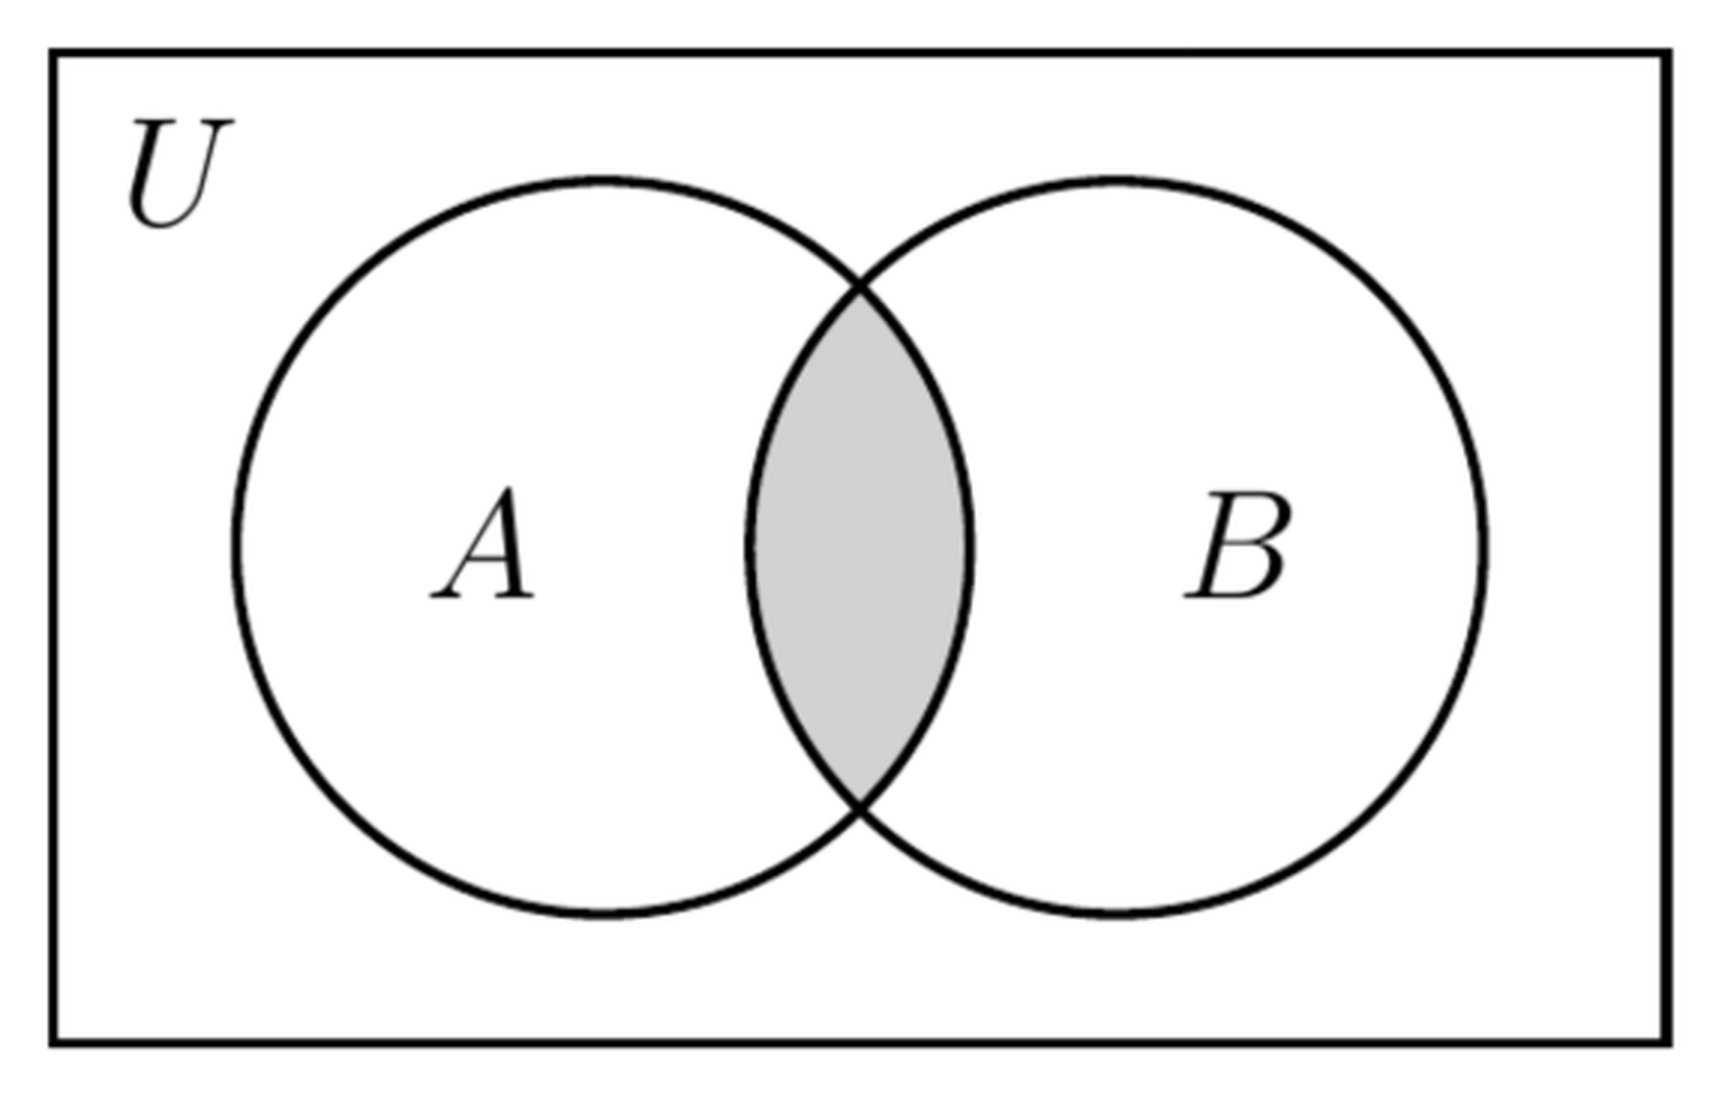
\includegraphics[width=0.38\textwidth]{figures/gao141_q5.png}
\end{center}

\ifanswer
\solbegin
\step{阴影部分表示 $A\cap B=\{4,7\}$.}
\solend
\fi

\item 方程 $2^{\log_3 x}=\dfrac12$ 的解集为\blankline[4.4em].

\ifanswer
\solbegin
\step{$2^{\log_3 x}=2^{-1}\Leftrightarrow\log_3 x=-1\Leftrightarrow x=\dfrac13$，解集为 $\left\{\dfrac13\right\}$.}
\solend
\fi

\item 若集合 $A=\left\{x\mid x^2+ax+\dfrac14=0\right\}$ 有且仅有两个子集，则实数 $a$ 的值为\blankline[4.4em].

\ifanswer
\solbegin
\step{$A$ 有且仅有两个子集，说明 $A$ 恰有一个元素，即方程有两个相等的实数根.}
\step{$\Delta=a^2-4\cdot\dfrac14=0\Rightarrow a=\pm1$.}% 判别式原卷印等腰偏高的高三角 $\Delta$，照录
\solend
\fi

\item 已知关于 $x$ 的方程 $x^2+mx+2m=0$ 的两个实数根分别为 $\alpha$、$\beta$，若 $\alpha^2+\beta^2=5$，则实数 $m=$\blankline[4.4em].

\ifanswer
\solbegin
\step{方程 $x^2+mx+2m=0$ 的两个实数根为 $\alpha$、$\beta$，}
\step{由根与系数的关系得 $\begin{cases}\alpha+\beta=-m\\\alpha\beta=2m\end{cases}$，又因为 $\alpha^2+\beta^2=5$，}
\step{所以 $\alpha^2+\beta^2=(\alpha+\beta)^2-2\alpha\beta=m^2-4m=5$，整理得 $m^2-4m-5=0$，}
\step{解得 $m=5$ 或 $m=-1$，}
\step{当 $m=5$ 时，$\triangle=25-40=-15<0$，无实根，舍去；}% 判别式原卷印扁等边三角 $\triangle$，照录
\step{当 $m=-1$ 时，$\triangle=1+8=9>0$，符合题意，}
\step{所以实数 $m=-1$.}
\solend
\fi

\item 若不等式 $\lvert x-3\rvert+\lvert x-5\rvert\geqslant a$ 对任意的实数 $x$ 恒成立，则实数 $a$ 的取值范围为\blankline[4.4em].

\ifanswer
\solbegin
\step{由三角不等式得 $\lvert x-3\rvert+\lvert x-5\rvert\geqslant\lvert x-3-x+5\rvert=2$，则 $a\leqslant2$.}
\solend
\fi

\item 设集合 $A=\{-3,2\}$，集合 $B=\{x\mid mx+1=0\}$，若 $A\cup B=A$，则实数 $m$ 的值为\blankline[4.4em].

\ifanswer
\solbegin
\step{由 $A\cup B=A$，得 $B\subseteq A$，}% 子集符号原卷印带下划线的 $\subseteq$，照录
\step{当 $m=0$ 时，$B=\varnothing$，满足题意，}
\step{当 $m\neq0$ 时，$B=\left\{-\dfrac1m\right\}$，所以 $-\dfrac1m=2$ 或 $-\dfrac1m=-3$，所以 $m=-\dfrac12$ 或 $m=\dfrac13$，}
\step{综上所述，$m=0$ 或 $m=-\dfrac12$ 或 $m=\dfrac13$.}
\solend
\fi

\item 已知 $m$ 为实数，代数式 $M=\sqrt{m-1}+\sqrt{3-m}$ 的取值范围为\blankline[4.4em].

\ifanswer
\solbegin
\step{根式有意义要求 $m\in[1,3]$，}
\step{此时 $(m-1)(3-m)=1-(m-2)^2$ 的取值范围为 $[0,1]$.}
\step{$M^2=2+2\sqrt{(m-1)(3-m)}$ 的取值范围为 $[2,4]$，又 $M>0$，}
\step{所以 $M\in[\sqrt2,2]$.}
\solend
\fi

\item 设有限集 $M$ 所含元素的个数用 $\mathbf{card}(M)$ 表示，并规定 $\mathbf{card}(\varnothing)=0$. 已知集合 $A,B$ 满足 $A\cup B=\{1,2,3\}$，$A\cap B=\varnothing$，若 $\mathbf{card}(A)\notin A$，$\mathbf{card}(B)\notin B$，则满足条件的所有不同集合 $A$ 的个数为\blankline[4.4em].

\ifanswer
\solbegin
\step{当 $\mathbf{card}(A)=0$ 或 $3$ 时，$A,B$ 中有一个为 $\{1,2,3\}$，不符合条件.}
\step{当 $\mathbf{card}(A)=1$ 时，$\mathbf{card}(B)=2\notin B$，所以 $A=\{2\}$，符合条件.}
\step{当 $\mathbf{card}(A)=2$ 时，$2\notin A$，所以 $B=\{2\}$，$A=\{1,3\}$，符合条件.}
\step{满足条件的集合 $A$ 共 $2$ 个.}
\solend
\fi

\end{enumerate}

\bigsec{二、选择题}

\begin{enumerate}
\setcounter{enumi}{12}

\item “ $x=1$ ” 是 “ $x^2-3x+2=0$ ” 的\mbox{（\quad）}条件.

\keepwithprev
A. 充分非必要\qquad B. 必要非充分

C. 充要\qquad D. 既非充分又非必要

\ifanswer
\solbegin
\step{$x^2-3x+2=0\Leftrightarrow x=1$ 或 $x=2$，所以 “ $x=1$ ” 是其充分非必要条件，}
\step{故选 $A$.}
\solend
\fi

\item 设 $a,b,c\in\R$，则下列命题为真命题的是\mbox{（\quad）}
% 原卷题干只声明 a,b,c，而 A 选项出现未声明的 d，照录（存疑）
\keepwithprev
A. 若 $a>b$ 且 $c>d$，则 $ac>bd$\qquad B. 若 $a^2>b^2$，则 $a>b$

C. 若 $ab>0$ 且 $a>b$，则 $\dfrac1a<\dfrac1b$\qquad D. 若 $a<0<b$，则 $\sqrt{-a}<\sqrt b$

\ifanswer
\solbegin
\step{$ab>0$ 且 $a>b\Rightarrow\dfrac1a-\dfrac1b=\dfrac{b-a}{ab}<0$，所以 $C$ 为真命题，故选 $C$.}
\solend
\fi

\item 已知 $\log_{14}7=a$，$14^b=5$，则 $\log_{35}28=$\mbox{（\quad）}

\keepwithprev
A. $\dfrac{2-a}{2a+b}$\qquad B. $\dfrac{2+a}{a+b}$\qquad C. $\dfrac{2-a}{a+2b}$\qquad D. $\dfrac{2-a}{a+b}$

\ifanswer
\solbegin
\step{$\log_{14}7=a$，$14^b=5$，}
\step{$\log_{35}28=\dfrac{\log_{14}28}{\log_{14}35}=\dfrac{\log_{14}14^2-\log_{14}7}{\log_{14}7+\log_{14}5}=\dfrac{2-a}{a+b}$. 故选 $D$.}
\solend
\fi

\item 关于 $x$ 的不等式 $ax^2+bx+3>0$ 的解集有下列说法，其中正确的个数是\mbox{（\quad）}

\keepwithprev
① 不等式 $ax^2+bx+3>0$ 的解集可以是 $\R$

② 不等式 $ax^2+bx+3>0$ 的解集可以是 $\{x\mid x>3\}$

③ 不等式 $ax^2+bx+3>0$ 的解集可以是 $\varnothing$

④ 不等式 $ax^2+bx+3>0$ 的解集可以是 $\{x\mid -1<x<3\}$

\keepwithprev
A. 4\qquad B. 3\qquad C. 2\qquad D. 1

\ifanswer
\solbegin
\step{$x=0$ 时左端为 $3>0$，解集必含 $0$，所以②③错误.}
\step{①取 $a=1,b=0$，$x^2+3>0$ 的解集为 $\R$，正确.}
\step{④取 $a=-1,b=2$，$-x^2+2x+3=-(x+1)(x-3)>0\Leftrightarrow-1<x<3$，正确.}
\step{正确的有①④，共 $2$ 个，故选 $C$.}
\solend
\fi

\end{enumerate}

\bigsec{三、解答题}

\begin{enumerate}
\setcounter{enumi}{16}

\item 已知集合 $A=\left\{x\mid\dfrac{x-2}{x+3}\geqslant0\right\}$，集合 $B=\{x\mid\lvert x+1\rvert+\lvert x-1\rvert<5\}$，全集 $U=\R$.

(1) 求 $A,B$；

(2) 求 $A\cup B$、$\overline{A\cap B}$.

\ifanswer
\solbegin
\step{(1) 分母不为零，且分子、分母同号或分子为零，}
\step{所以 $\dfrac{x-2}{x+3}\geqslant0\Leftrightarrow x<-3$ 或 $x\geqslant2$，因此 $A=(-\infty,-3)\cup[2,+\infty)$.}
\step{又 $\lvert x+1\rvert+\lvert x-1\rvert=\begin{cases}-2x,&x<-1\\2,&-1\leqslant x\leqslant1\\2x,&x>1\end{cases}$，}
\step{分别解得 $-\dfrac52<x<-1$、$-1\leqslant x\leqslant1$、$1<x<\dfrac52$，因此 $B=\left(-\dfrac52,\dfrac52\right)$.}
\step{(2) 合并两集合所对应的区间，得 $A\cup B=(-\infty,-3)\cup\left(-\dfrac52,+\infty\right)$，}
\step{两集合的公共部分为 $A\cap B=\left[2,\dfrac52\right)$，所以 $\overline{A\cap B}=(-\infty,2)\cup\left[\dfrac52,+\infty\right)$.}
\solend
\fi

\item (1) 已知 $a>b>0$，比较代数式 $\dfrac ab$ 与 $\dfrac{a+1}{b+1}$ 的大小并说明理由；

(2) 已知 $x,y,z$ 都是正实数，$a=x+\dfrac1y,b=y+\dfrac1z,c=z+\dfrac1x$，试用反证法证明 $a,b,c$ 至少有一个不小于 $2$.

\ifanswer
\solbegin
\step{(1) $\dfrac ab-\dfrac{a+1}{b+1}=\dfrac{a(b+1)-b(a+1)}{b(b+1)}=\dfrac{a-b}{b(b+1)}$，}
\step{因为 $a>b>0$，所以 $a-b>0$，$b(b+1)>0$，所以 $\dfrac ab-\dfrac{a+1}{b+1}>0$，}
\step{故 $\dfrac ab>\dfrac{a+1}{b+1}$.}
\step{(2) 假设 $a$、$b$、$c$ 三数都小于 $2$，则 $x+\dfrac1y+y+\dfrac1z+z+\dfrac1x<6$.}
\step{因为 $x,y,z$ 均大于 $0$，}
\step{所以 $x+\dfrac1y+y+\dfrac1z+z+\dfrac1x=x+\dfrac1x+y+\dfrac1y+z+\dfrac1z\geqslant2+2+2=6$，矛盾，}
\step{所以 $a$、$b$、$c$ 三数中至少有一个不小于 $2$.}
\solend
\fi

% 第 19 题长方体无盖贮水池砖墙示意图（题目配图，三版都出）：取原卷 06 页截图去粉色水印、LANCZOS 放大 3 倍
\needvspace{6cm}
\item 如图所示，某工厂要建造一个长方体形无盖贮水池，其容积为 $3200m^3$，深为 $2m$.

(1) 若水池的长比宽至少多 $60m$，求水池的宽的最大值；

(2) 若池底每平方米的造价为 $150$ 元，池壁每平方米的造价为 $120$ 元，那么怎样设计水池的长和宽能使总造价最低？最低总造价是多少？

\begin{center}
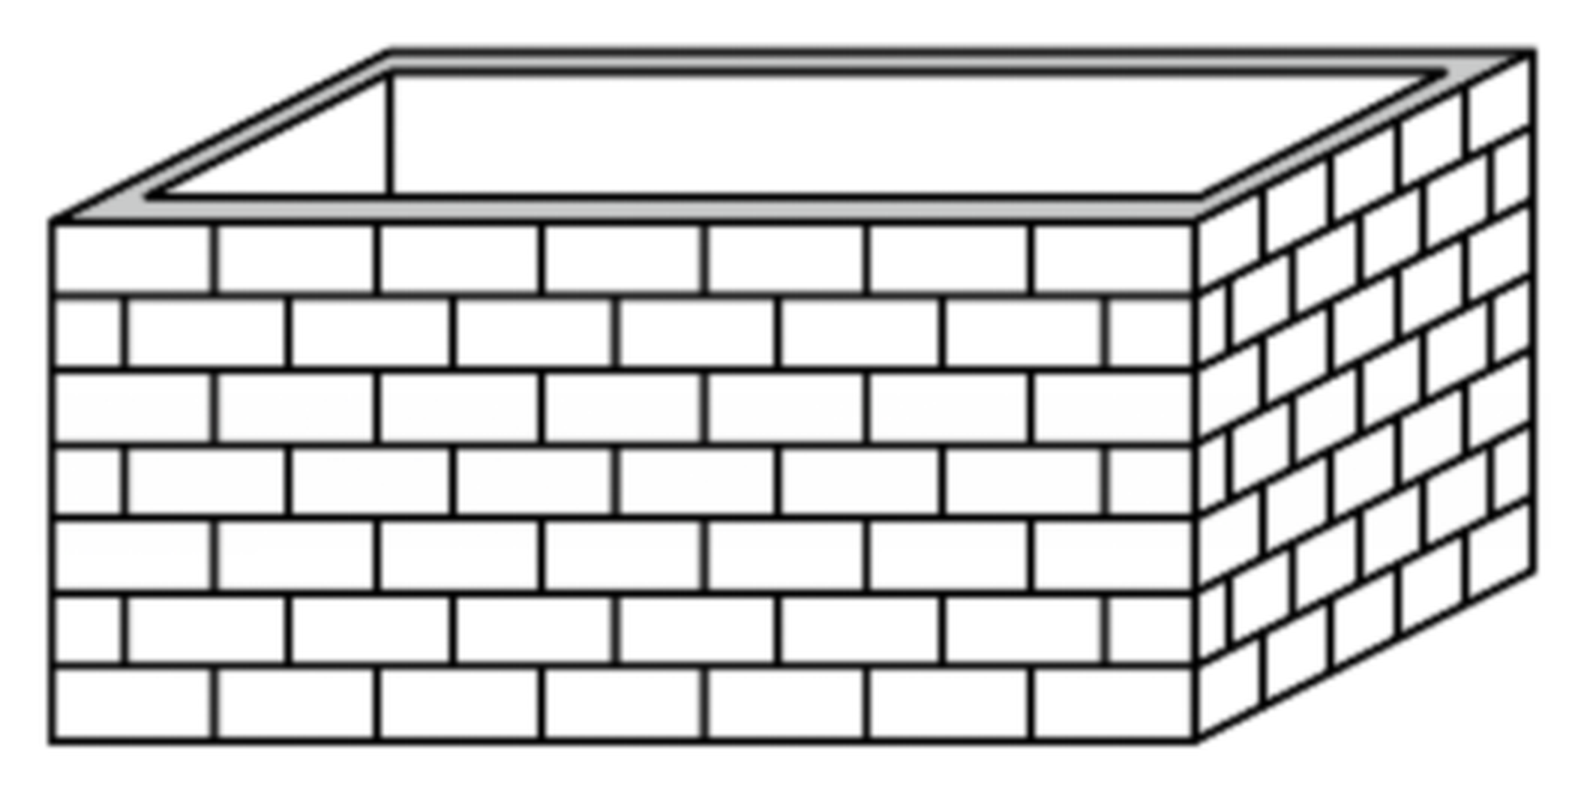
\includegraphics[width=0.42\textwidth]{figures/gao141_q19.png}
\end{center}

\ifanswer
\solbegin
\step{(1) 设水池的长、宽分别为 $xm$，$ym$，则 $x-y\geqslant60$，且 $x$、$y>0$，}
\step{由题意得 $2xy=3200$，即 $x=\dfrac{1600}{y}$，所以 $\dfrac{1600}{y}-y\geqslant60$，}
\step{因为 $y>0$，所以 $1600-y^2\geqslant60y$，}
\step{即 $y^2+60y-1600=(y+80)(y-20)\leqslant0$，解得 $-80\leqslant y\leqslant20$，}
\step{又 $y>0$，所以 $0<y\leqslant20$，所以水池的宽的最大值为 $20m$.}
\step{(2) 设水池总造价为 $z$ 元，}
\step{则 $z=1600\times150+2\times(2x+2y)\times120=240000+480(x+y)$，}
\step{又因为 $y=\dfrac{1600}{x}$，}
\step{所以 $z=240000+\left(x+\dfrac{1600}{x}\right)\times480\geqslant240000+480\times2\sqrt{1600}$}
\step{$=240000+38400=278400$，}
\step{当且仅当 $x=\dfrac{1600}{x}$，即 $x=y=40$ 时取等号，}
\step{所以，将水池的池底设计为边长为 $40m$ 的正方形时总造价最低，}
\step{最低总造价为 $278400$ 元.}
\solend
\fi

\item 已知 $a\in\R$，设集合 $A=\{x\mid ax^2-3x+2<ax-1\}$.

(1) 若 $A=(1,3)$，求实数 $a$ 的值；

(2) 当 $a>0$ 时，求 $A$；

(3) 若 “ $x\in\left(\dfrac12,+\infty\right)$ ” 是 “ $x\in A$ ” 的必要非充分条件，求实数 $a$ 的取值范围.

\ifanswer
\solbegin
\step{原不等式等价于 $ax^2-(a+3)x+3<0\Leftrightarrow(x-1)(ax-3)<0$，}
\step{(1) $A=(1,3)$ 为有界区间，因此 $a>0$，两根为 $1$ 和 $\dfrac3a$，于是 $\dfrac3a=3$，得 $a=1$；}
\step{此时 $(x-1)(x-3)<0$ 的解集确为 $(1,3)$.}
\step{(2) 当 $a>0$ 时，二次项系数为正，比较 $1$ 与 $\dfrac3a$，得 $A=\begin{cases}\left(1,\dfrac3a\right),&0<a<3\\\varnothing,&a=3\\\left(\dfrac3a,1\right),&a>3\end{cases}$，}
\step{其中 $a=3$ 时，原不等式为 $3(x-1)^2<0$，无解.}
\step{(3) 记 $S=\left(\dfrac12,+\infty\right)$，题意要求 $A\subset S$.}% 子集符号原卷印单线 $\subset$，照录
\step{由于对任意 $a$ 都有 $1\notin A$，而 $1\in S$，所以只需满足 $A\subseteq S$.}
\step{当 $a<0$ 时，$A=\left(-\infty,\dfrac3a\right)\cup(1,+\infty)$，含有小于 $\dfrac12$ 的数，不符合条件.}
\step{当 $a=0$ 时，$A=(1,+\infty)$，符合条件.}
\step{当 $0<a<3$ 时，$A=\left(1,\dfrac3a\right)\subseteq S$；}
\step{当 $a=3$ 时，$A=\varnothing\subseteq S$，均符合条件；}
\step{当 $a>3$ 时，$A=\left(\dfrac3a,1\right)$，所以 $A\subseteq S\Leftrightarrow\dfrac3a\geqslant\dfrac12\Leftrightarrow a\leqslant6$；}
\step{因此实数 $a$ 的取值范围为 $[0,6]$.}
\solend
\fi

\item 甲、乙两同学探讨了一个问题：已知正实数 $x,y$ 满足 $3x+y=1$，求 $\dfrac1x+\dfrac1y$ 的最小值.

甲给出的解法：由 $1=3x+y\geqslant2\sqrt{3xy}$，得 $\sqrt{xy}\leqslant\dfrac{\sqrt3}{6}$，所以 $\dfrac1x+\dfrac1y\geqslant2\sqrt{\dfrac1{xy}}\geqslant4\sqrt3$. 因此 $\dfrac1x+\dfrac1y$ 的最小值为 $4\sqrt3$.

乙给出的解法：$\dfrac1x+\dfrac1y=\left(\dfrac1x+\dfrac1y\right)(3x+y)=4+\dfrac yx+\dfrac{3x}{y}$，因为 $x,y$ 均为正实数，所以 $\dfrac1x+\dfrac1y\geqslant4+2\sqrt{\dfrac yx\cdot\dfrac{3x}{y}}=4+2\sqrt3$.

(1) 请判断上述哪位同学的解法正确，哪位同学的解法错误，并指出错误的原因；

(2) 结合上述探讨，试求当 $0<x<\dfrac12$ 时，$\dfrac1x+\dfrac1{1-2x}$ 的最小值以及此时实数 $x$ 的值；

(3) 已知 $x$ 为正实数，$y$ 为非负实数，且 $x+2y=2$，求 $\dfrac{x^2+1}{x}+\dfrac{2y^2}{y+1}$ 的最小值以及此时实数 $x,y$ 的值.

\ifanswer
\solbegin
\step{(1) 甲的推导中，$3x+y\geqslant2\sqrt{3xy}$ 取等号要求 $3x=y$，}
\step{$\dfrac1x+\dfrac1y\geqslant\dfrac2{\sqrt{xy}}$ 取等号要求 $x=y$，两者对正实数 $x,y$ 不能同时成立，}
\step{因此不能将 $4\sqrt3$ 判为最小值，甲错误.}
\step{乙的等号条件为 $\dfrac yx=\dfrac{3x}{y}$，即 $y=\sqrt3 x$；}
\step{结合 $3x+y=1$，得 $x=\dfrac1{3+\sqrt3},y=\dfrac{\sqrt3}{3+\sqrt3}$ 均为正数，等号可以成立，}
\step{因此乙正确，最小值为 $4+2\sqrt3$.}
\step{(2) 令 $t=1-2x>0$，则 $2x+t=1$.}
\step{$\dfrac1x+\dfrac1t=\left(\dfrac1x+\dfrac1t\right)(2x+t)=3+\dfrac tx+\dfrac{2x}{t}\geqslant3+2\sqrt2$，}
\step{当且仅当 $\dfrac tx=\dfrac{2x}{t}$，即 $t=\sqrt2 x$ 时取等号，}
\step{由 $2x+t=1$，得 $x=\dfrac1{2+\sqrt2}=\dfrac{2-\sqrt2}{2}\in\left(0,\dfrac12\right)$，}
\step{因此最小值为 $3+2\sqrt2$，此时 $x=\dfrac{2-\sqrt2}{2}$.}
\step{(3) 记目标式为 $F$，利用 $x+2y=2$，}
\step{得 $F=x+\dfrac1x+2y-2+\dfrac2{y+1}=\dfrac1x+\dfrac2{y+1}$，}
\step{又 $x+2(y+1)=4$，且 $x>0$、$y+1>0$，}
\step{所以 $4F=\left(\dfrac1x+\dfrac2{y+1}\right)(x+2(y+1))=5+2\left(\dfrac{y+1}{x}+\dfrac{x}{y+1}\right)$}
\step{$\geqslant5+2\times2=9$，当且仅当 $\dfrac{y+1}{x}=\dfrac{x}{y+1}$，即 $x=y+1$ 时取等号.}
\step{联立 $x+2y=2$，得 $x=\dfrac43$、$y=\dfrac13$，满足题设条件，}
\step{因此最小值为 $\dfrac94$，此时 $x=\dfrac43$，$y=\dfrac13$.}
\solend
\fi

\end{enumerate}

\end{document}
"
% 紧凑版：xelatex "\def\iscompact{1}% 高一141_彭浦中学_期中.tex
%   —— 高一上数学"2026-2027 年彭浦中学高一上期中"（试卷版/答案版/紧凑版）
% 试卷版：xelatex 高一141_彭浦中学_期中.tex
% 答案版：xelatex "\def\isanswer{1}% 高一141_彭浦中学_期中.tex
%   —— 高一上数学"2026-2027 年彭浦中学高一上期中"（试卷版/答案版/紧凑版）
% 试卷版：xelatex 高一141_彭浦中学_期中.tex
% 答案版：xelatex "\def\isanswer{1}\input{高一141_彭浦中学_期中.tex}"
% 紧凑版：xelatex "\def\iscompact{1}\input{高一141_彭浦中学_期中.tex}"
%
% ① 原始材料：微信公众号"魔都数学加油站"文章，连载"27学年高一141"，原文标题
% "27学年高一141——2026-2027年上海市彭浦中学高一上期中"；
% 原文链接：https://mp.weixin.qq.com/s/V_8bEhC6geeFyQysmtqUtQ。
% 正文为 9 张 PNG 页（01、05、06、07、09 为 2560x3620；02、03、04、08 为 4762x6735，
% 同一篇各页分辨率不同，逐页按各自分辨率放大裁图核对），题目下印【解析】，为讲评版。
% 题目、解析均据原图转录；卷面粉红色水印"魔都数学加油站"及公众号页脚未录入。
% 全卷 2 幅插图，均属题目配图（在 \ifanswer 外、三版都出）、取原卷截图去粉色水印、
% LANCZOS 放大 3 倍：第 5 题韦恩图（01 页，全集 U 矩形内两圆相交、交集阴影、A/B/U 标注）、
% 第 19 题长方体无盖贮水池砖墙示意图（06 页右上）。通读 9 页确认除这 2 幅外无其它
% 插图/表格，亦无"题干写如图而源码漏图"（仅 Q5"图中阴影部分"、Q19"如图所示"两处提到图）。
%
% 卷首标题：原卷印作"2026-2027 年彭浦中学高一上期中"（公众号标题中的"上海市"
% 卷面标题行没有，本稿照卷面），年份区间按全稿惯例排 en dash；原卷未印副标题，
% 本卷为期中卷、跨集合与常用逻辑用语／不等式／函数三章，按题目内容补出
% "集合与常用逻辑用语、不等式、函数"（与 高一140 同期中卷口径相同）：
% 集合与逻辑见 Q5、Q10、Q12、Q13、Q16、Q17、Q20，不等式见 Q4、Q9、Q14、Q18、
% Q19、Q21，函数（指数／对数）见 Q6、Q15。
%
% 题号体例：本卷共 19 题——一、填空题 3—12（10 题）、二、选择题 13—16（4 题）、
% 三、解答题 17—21（5 题）。三节分别 \setcounter{enumi}{2}／{12}／{16}。
% 原卷从第 3 题起、无第 1、2 题，本稿保留原题号；全卷无附加题节。
%
% ② 与原卷的排版差异：
%   ① 原文从第 3 题起，本稿保留原题号；
%   ② 原卷 19 题题下均印【解析】，无独立【答案】段、无"答案印题干括号且无解析"、
%      无"只印【答案】无解析"一型：填空题与解答题的答案落在【解析】末句
%      （Q3—Q12、Q17—Q21），四道选择题答案在【解析】末句"故选 …"
%      （Q13 选 A、Q14 选 C、Q15 选 D、Q16 选 C），题干括号内一律留空；
%      本稿 19 题一律 \solbegin…\solend、全卷不提 \ans{}，答案版【解析】标记数
%      = 19 = 全卷题数（无【答案】标记）；
%   ③ 原卷未印副标题，本稿按"知识模块"口径补出；
%   ④ 原卷填空横线按全稿惯例排 \blankline[4.4em]；选择题括号排 \mbox{（\quad）}，
%      选项段／命题段前按惯例加 \keepwithprev（Q16 两枚：命题列与选项段各一）；
%      解答题不留作答区、不加 \anspace（原卷为讲评版，与 129／131／132／133／136／140 同）；
%   ⑤ 原卷数集混排：黑板粗体 R（Q14 题干、Q16 ① 与解析、Q17 全集、Q20 题干）
%      按全稿惯例统一改 \R；空集记号 \varnothing；绝对值排 \lvert…\rvert，
%      集合描述竖线排 \mid；不等号按全稿惯例排 \leqslant／\geqslant；
%      补集照原卷上划线排 \overline{A\cap B}（Q17(2) 题干与解析）；
%      原卷"card"记号排黑体正体（Q12），本稿照录 \mathbf{card}，未改斜体
%      （与 高一66 同题口径不同：那份原卷 card 排斜体、照录 $card(M)$）；
%   ⑥ 子题标号 (1)(2)(3) 原卷印半角括号，照录；圈数字 ①②③④ 在正文（文本模式）
%      按原卷照录，未进数学式；数学式内半角逗号照录（如 Q12"$A,B$"、"{1,2,3}"、
%      Q14"$a,b,c\in\R$"、Q15"$\log_{14}7=a$，$14^b=5$"、Q16"$a=1,b=0$"、
%      Q18"$x,y,z$"、Q20"$x,y$"、Q21"$x,y$"）；全卷行末西文句点照录为 ASCII 句点；
%      行中全角逗号、顿号照录；
%   ⑦ 题干中的中文弯引号按原卷照录（Q13、Q20(3) 的 “ ” 及引号内空格），
%      注释内一律 ASCII 引号；
%   ⑧ 两幅题目配图各在 \item 之前加 \needvspace 守卫整块推走（Q5 5cm、Q19 6cm），
%      守卫放在 \item 之前而非 \bigsec 之后——两题均非各节首题，不触发 B 类
%      "节标题落页末"（照 高一26／40／59／136／140 成例）；三版切页审计均"合计异常：无"；
%   ⑨ 跨页续印按题合并：Q8 题干与【解析】首行在 01 页、后 6 行在 02 页；
%      Q15 题干在 03 页、【解析】在 04 页；Q17 题干与【解析】前 2 行在 04 页、
%      后 4 行在 05 页；Q19 题干在 05 页末、(1)(2) 小问与砖墙图与【解析】在 06 页；
%      Q20 题干 (1)(2) 在 06 页末、(3) 与【解析】在 07 页；Q21 题干与【解析】
%      前 6 行在 08 页、后 12 行在 09 页；Q16、Q18 全在各自页内；
%      本稿按题连排，不丢行；
%   ⑩ 原卷无红色加粗标签（【解析】均黑色印刷，Q16 解析 "①取…""④取…" 与
%      Q20 解析 "(2)" 等分步标签亦黑色），故本卷未用 \stepm；
%   ⑪ 原卷 Q19 题干把数值与单位（3200m³、2m、60m、150 元、120 元、40m、20m、
%      278400 元）印作略粗的西文字形，本稿按全稿惯例（高一70／72 同类题）排普通
%      数学体，未加粗。
%
% ③ 行数复核：一条 \step = 原卷解析的一个印刷行，cases 块作一个印刷行计。逐题数 \step
%   条数，合计 92 条（Q3：1；Q4：1；Q5：1；Q6：1；Q7：2；Q8：7；Q9：1；Q10：4；
%   Q11：4；Q12：4；Q13：2；Q14：1；Q15：2；Q16：4；Q17：6；Q18：7；Q19：13；
%   Q20：13；Q21：18），与原卷印刷行逐题相等。全卷 19 题均印【解析】、无独立 \ans{}，
%   答案版【解析】标记数 = 19 = 全卷题数。
%
% ④ 判别式／子集符号结论（逐处放大原图照录、不得统一）：
%   判别式：全卷 3 处——第 7 题【解析】"$\Delta=a^2-4\cdot\frac14=0$"一处原卷印
%     等腰、偏高的高三角 $\Delta$，照录 \Delta；第 8 题【解析】
%     "$\triangle=25-40=-15<0$"与"$\triangle=1+8=9>0$"两处原卷印扁等边三角
%     $\triangle$，照录 \triangle。两形不同，逐处照录未统一。
%   子集：全卷 6 处——第 10 题【解析】"$B\subseteq A$"一处、第 20 题【解析】
%     "所以只需满足 $A\subseteq S$"、"$A=\left(1,\frac3a\right)\subseteq S$"、
%     "$A=\varnothing\subseteq S$"、"$A\subseteq S\Leftrightarrow\frac3a\geqslant\frac12$"
%     四处，共 5 处原卷印带下划线的 $\subseteq$，照录 \subseteq；第 20 题【解析】
%     (3) 首行"题意要求 $A\subset S$"一处原卷印单线 $\subset$，照录 \subset
%     （下行因 $1\in S$ 而 $1\notin A$，改述为 $A\subseteq S$，两者逻辑一致、非笔误）。
%
% ⑤ 存疑照录（照录未改，正文对应处另有 % 注）：
%   第 14 题题干"设 $a,b,c\in\R$"只声明 $a,b,c$，而 A 选项"若 $a>b$ 且 $c>d$，
%     则 $ac>bd$"引入未声明的 $d$，原卷变量声明与选项不统一，照录未补。
%   全卷除此 1 条外未发现其它笔误／自相矛盾处。
%
% ⑥ 跨页续印按题合并说明：见 ② ⑨。
%
\documentclass[a4paper,11pt]{article}
\usepackage{common}

\begin{document}

\examtitlest[3]{2026--2027 年彭浦中学高一上期中}{集合与常用逻辑用语、不等式、函数}

\bigsec{一、填空题}

\begin{enumerate}
\setcounter{enumi}{2}

\item 已知 $m$ 为实数，若 $1\in\{m,m^2\}$，则 $m$ 的值为\blankline[4.4em].

\ifanswer
\solbegin
\step{$m=1$ 或 $m^2=1$，得 $m=\pm1$；按列举项互异口径排除 $m=m^2=1$，得 $m=-1$.}
\solend
\fi

\item 已知 $2<a<4$，$-2<b<1$，则 $2a+b$ 的取值范围为\blankline[4.4em].

\ifanswer
\solbegin
\step{$4<2a<8$，与 $-2<b<1$ 相加，得 $2<2a+b<9$，取值范围为 $(2,9)$.}
\solend
\fi

% 第 5 题韦恩图（题目配图，三版都出）：取原卷 01 页截图去粉色水印、LANCZOS 放大 3 倍
\needvspace{5cm}
\item 已知集合 $A=\{-1,-2,1,4,7\}$，$B=\{x\mid x>1\}$，用列举法表示图中阴影部分所表示的集合为\blankline[4.4em].

\begin{center}
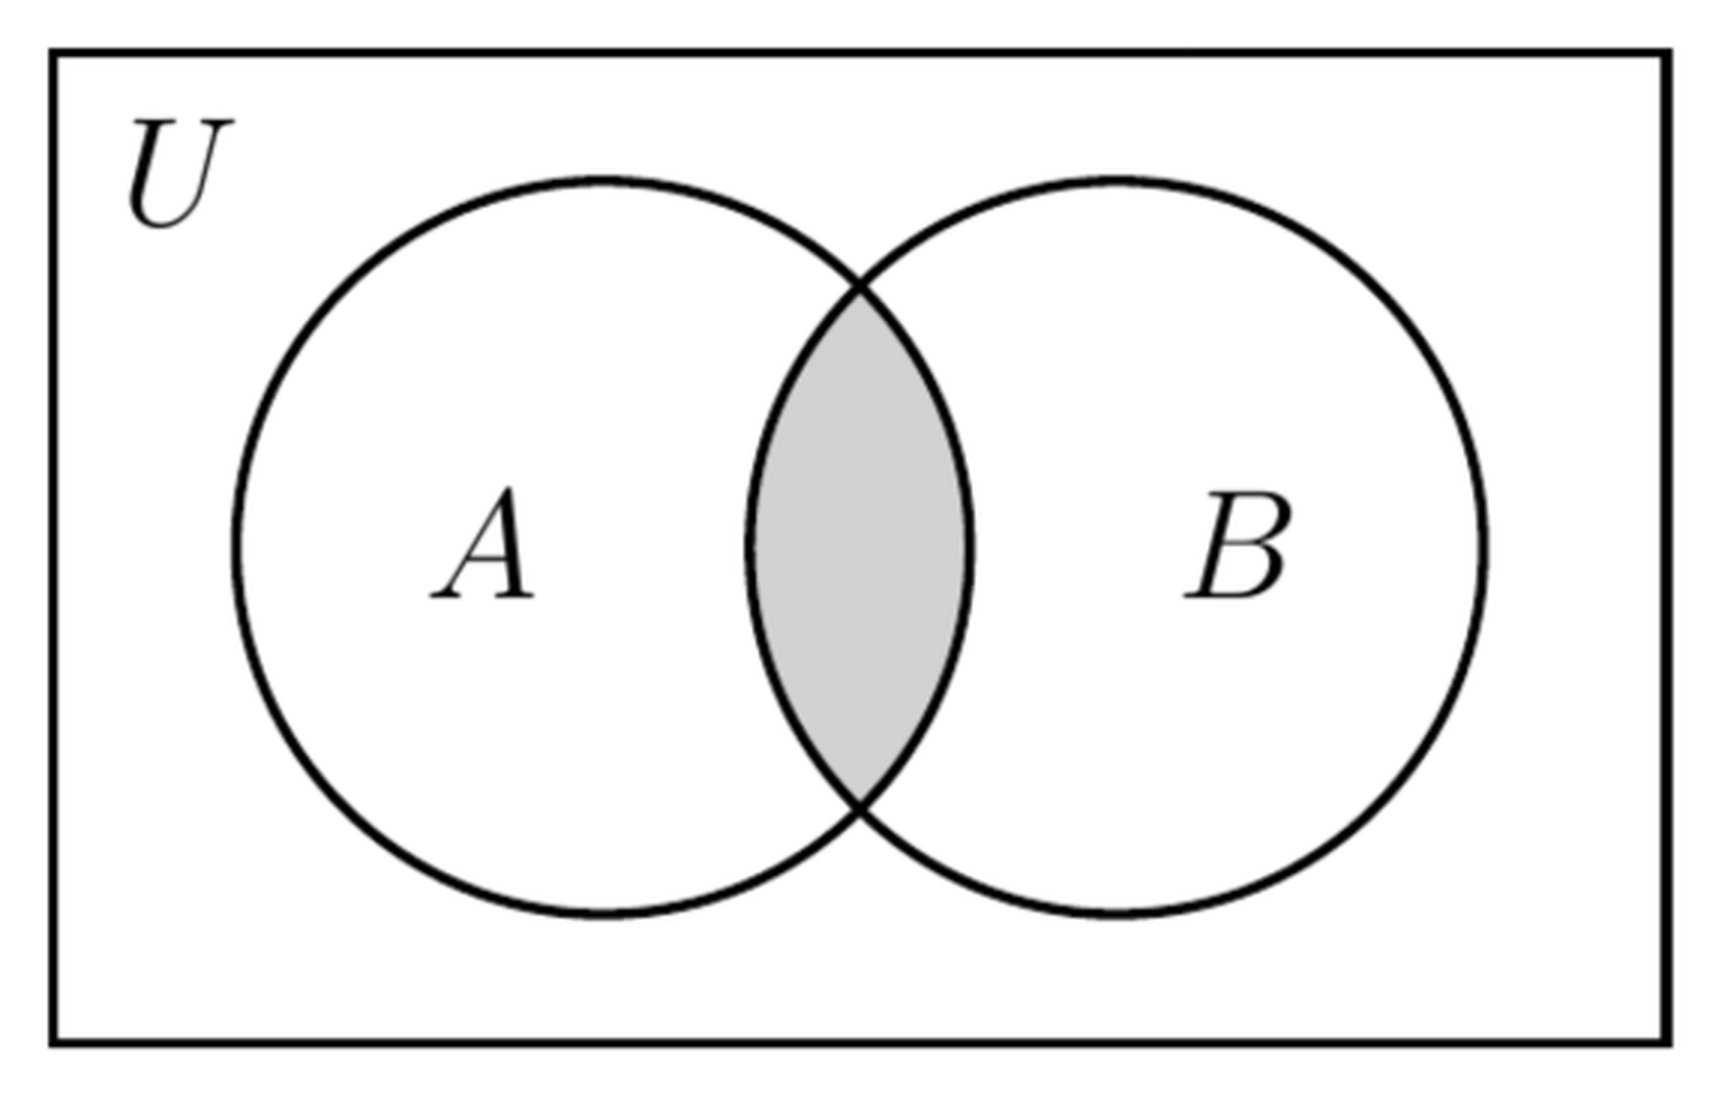
\includegraphics[width=0.38\textwidth]{figures/gao141_q5.png}
\end{center}

\ifanswer
\solbegin
\step{阴影部分表示 $A\cap B=\{4,7\}$.}
\solend
\fi

\item 方程 $2^{\log_3 x}=\dfrac12$ 的解集为\blankline[4.4em].

\ifanswer
\solbegin
\step{$2^{\log_3 x}=2^{-1}\Leftrightarrow\log_3 x=-1\Leftrightarrow x=\dfrac13$，解集为 $\left\{\dfrac13\right\}$.}
\solend
\fi

\item 若集合 $A=\left\{x\mid x^2+ax+\dfrac14=0\right\}$ 有且仅有两个子集，则实数 $a$ 的值为\blankline[4.4em].

\ifanswer
\solbegin
\step{$A$ 有且仅有两个子集，说明 $A$ 恰有一个元素，即方程有两个相等的实数根.}
\step{$\Delta=a^2-4\cdot\dfrac14=0\Rightarrow a=\pm1$.}% 判别式原卷印等腰偏高的高三角 $\Delta$，照录
\solend
\fi

\item 已知关于 $x$ 的方程 $x^2+mx+2m=0$ 的两个实数根分别为 $\alpha$、$\beta$，若 $\alpha^2+\beta^2=5$，则实数 $m=$\blankline[4.4em].

\ifanswer
\solbegin
\step{方程 $x^2+mx+2m=0$ 的两个实数根为 $\alpha$、$\beta$，}
\step{由根与系数的关系得 $\begin{cases}\alpha+\beta=-m\\\alpha\beta=2m\end{cases}$，又因为 $\alpha^2+\beta^2=5$，}
\step{所以 $\alpha^2+\beta^2=(\alpha+\beta)^2-2\alpha\beta=m^2-4m=5$，整理得 $m^2-4m-5=0$，}
\step{解得 $m=5$ 或 $m=-1$，}
\step{当 $m=5$ 时，$\triangle=25-40=-15<0$，无实根，舍去；}% 判别式原卷印扁等边三角 $\triangle$，照录
\step{当 $m=-1$ 时，$\triangle=1+8=9>0$，符合题意，}
\step{所以实数 $m=-1$.}
\solend
\fi

\item 若不等式 $\lvert x-3\rvert+\lvert x-5\rvert\geqslant a$ 对任意的实数 $x$ 恒成立，则实数 $a$ 的取值范围为\blankline[4.4em].

\ifanswer
\solbegin
\step{由三角不等式得 $\lvert x-3\rvert+\lvert x-5\rvert\geqslant\lvert x-3-x+5\rvert=2$，则 $a\leqslant2$.}
\solend
\fi

\item 设集合 $A=\{-3,2\}$，集合 $B=\{x\mid mx+1=0\}$，若 $A\cup B=A$，则实数 $m$ 的值为\blankline[4.4em].

\ifanswer
\solbegin
\step{由 $A\cup B=A$，得 $B\subseteq A$，}% 子集符号原卷印带下划线的 $\subseteq$，照录
\step{当 $m=0$ 时，$B=\varnothing$，满足题意，}
\step{当 $m\neq0$ 时，$B=\left\{-\dfrac1m\right\}$，所以 $-\dfrac1m=2$ 或 $-\dfrac1m=-3$，所以 $m=-\dfrac12$ 或 $m=\dfrac13$，}
\step{综上所述，$m=0$ 或 $m=-\dfrac12$ 或 $m=\dfrac13$.}
\solend
\fi

\item 已知 $m$ 为实数，代数式 $M=\sqrt{m-1}+\sqrt{3-m}$ 的取值范围为\blankline[4.4em].

\ifanswer
\solbegin
\step{根式有意义要求 $m\in[1,3]$，}
\step{此时 $(m-1)(3-m)=1-(m-2)^2$ 的取值范围为 $[0,1]$.}
\step{$M^2=2+2\sqrt{(m-1)(3-m)}$ 的取值范围为 $[2,4]$，又 $M>0$，}
\step{所以 $M\in[\sqrt2,2]$.}
\solend
\fi

\item 设有限集 $M$ 所含元素的个数用 $\mathbf{card}(M)$ 表示，并规定 $\mathbf{card}(\varnothing)=0$. 已知集合 $A,B$ 满足 $A\cup B=\{1,2,3\}$，$A\cap B=\varnothing$，若 $\mathbf{card}(A)\notin A$，$\mathbf{card}(B)\notin B$，则满足条件的所有不同集合 $A$ 的个数为\blankline[4.4em].

\ifanswer
\solbegin
\step{当 $\mathbf{card}(A)=0$ 或 $3$ 时，$A,B$ 中有一个为 $\{1,2,3\}$，不符合条件.}
\step{当 $\mathbf{card}(A)=1$ 时，$\mathbf{card}(B)=2\notin B$，所以 $A=\{2\}$，符合条件.}
\step{当 $\mathbf{card}(A)=2$ 时，$2\notin A$，所以 $B=\{2\}$，$A=\{1,3\}$，符合条件.}
\step{满足条件的集合 $A$ 共 $2$ 个.}
\solend
\fi

\end{enumerate}

\bigsec{二、选择题}

\begin{enumerate}
\setcounter{enumi}{12}

\item “ $x=1$ ” 是 “ $x^2-3x+2=0$ ” 的\mbox{（\quad）}条件.

\keepwithprev
A. 充分非必要\qquad B. 必要非充分

C. 充要\qquad D. 既非充分又非必要

\ifanswer
\solbegin
\step{$x^2-3x+2=0\Leftrightarrow x=1$ 或 $x=2$，所以 “ $x=1$ ” 是其充分非必要条件，}
\step{故选 $A$.}
\solend
\fi

\item 设 $a,b,c\in\R$，则下列命题为真命题的是\mbox{（\quad）}
% 原卷题干只声明 a,b,c，而 A 选项出现未声明的 d，照录（存疑）
\keepwithprev
A. 若 $a>b$ 且 $c>d$，则 $ac>bd$\qquad B. 若 $a^2>b^2$，则 $a>b$

C. 若 $ab>0$ 且 $a>b$，则 $\dfrac1a<\dfrac1b$\qquad D. 若 $a<0<b$，则 $\sqrt{-a}<\sqrt b$

\ifanswer
\solbegin
\step{$ab>0$ 且 $a>b\Rightarrow\dfrac1a-\dfrac1b=\dfrac{b-a}{ab}<0$，所以 $C$ 为真命题，故选 $C$.}
\solend
\fi

\item 已知 $\log_{14}7=a$，$14^b=5$，则 $\log_{35}28=$\mbox{（\quad）}

\keepwithprev
A. $\dfrac{2-a}{2a+b}$\qquad B. $\dfrac{2+a}{a+b}$\qquad C. $\dfrac{2-a}{a+2b}$\qquad D. $\dfrac{2-a}{a+b}$

\ifanswer
\solbegin
\step{$\log_{14}7=a$，$14^b=5$，}
\step{$\log_{35}28=\dfrac{\log_{14}28}{\log_{14}35}=\dfrac{\log_{14}14^2-\log_{14}7}{\log_{14}7+\log_{14}5}=\dfrac{2-a}{a+b}$. 故选 $D$.}
\solend
\fi

\item 关于 $x$ 的不等式 $ax^2+bx+3>0$ 的解集有下列说法，其中正确的个数是\mbox{（\quad）}

\keepwithprev
① 不等式 $ax^2+bx+3>0$ 的解集可以是 $\R$

② 不等式 $ax^2+bx+3>0$ 的解集可以是 $\{x\mid x>3\}$

③ 不等式 $ax^2+bx+3>0$ 的解集可以是 $\varnothing$

④ 不等式 $ax^2+bx+3>0$ 的解集可以是 $\{x\mid -1<x<3\}$

\keepwithprev
A. 4\qquad B. 3\qquad C. 2\qquad D. 1

\ifanswer
\solbegin
\step{$x=0$ 时左端为 $3>0$，解集必含 $0$，所以②③错误.}
\step{①取 $a=1,b=0$，$x^2+3>0$ 的解集为 $\R$，正确.}
\step{④取 $a=-1,b=2$，$-x^2+2x+3=-(x+1)(x-3)>0\Leftrightarrow-1<x<3$，正确.}
\step{正确的有①④，共 $2$ 个，故选 $C$.}
\solend
\fi

\end{enumerate}

\bigsec{三、解答题}

\begin{enumerate}
\setcounter{enumi}{16}

\item 已知集合 $A=\left\{x\mid\dfrac{x-2}{x+3}\geqslant0\right\}$，集合 $B=\{x\mid\lvert x+1\rvert+\lvert x-1\rvert<5\}$，全集 $U=\R$.

(1) 求 $A,B$；

(2) 求 $A\cup B$、$\overline{A\cap B}$.

\ifanswer
\solbegin
\step{(1) 分母不为零，且分子、分母同号或分子为零，}
\step{所以 $\dfrac{x-2}{x+3}\geqslant0\Leftrightarrow x<-3$ 或 $x\geqslant2$，因此 $A=(-\infty,-3)\cup[2,+\infty)$.}
\step{又 $\lvert x+1\rvert+\lvert x-1\rvert=\begin{cases}-2x,&x<-1\\2,&-1\leqslant x\leqslant1\\2x,&x>1\end{cases}$，}
\step{分别解得 $-\dfrac52<x<-1$、$-1\leqslant x\leqslant1$、$1<x<\dfrac52$，因此 $B=\left(-\dfrac52,\dfrac52\right)$.}
\step{(2) 合并两集合所对应的区间，得 $A\cup B=(-\infty,-3)\cup\left(-\dfrac52,+\infty\right)$，}
\step{两集合的公共部分为 $A\cap B=\left[2,\dfrac52\right)$，所以 $\overline{A\cap B}=(-\infty,2)\cup\left[\dfrac52,+\infty\right)$.}
\solend
\fi

\item (1) 已知 $a>b>0$，比较代数式 $\dfrac ab$ 与 $\dfrac{a+1}{b+1}$ 的大小并说明理由；

(2) 已知 $x,y,z$ 都是正实数，$a=x+\dfrac1y,b=y+\dfrac1z,c=z+\dfrac1x$，试用反证法证明 $a,b,c$ 至少有一个不小于 $2$.

\ifanswer
\solbegin
\step{(1) $\dfrac ab-\dfrac{a+1}{b+1}=\dfrac{a(b+1)-b(a+1)}{b(b+1)}=\dfrac{a-b}{b(b+1)}$，}
\step{因为 $a>b>0$，所以 $a-b>0$，$b(b+1)>0$，所以 $\dfrac ab-\dfrac{a+1}{b+1}>0$，}
\step{故 $\dfrac ab>\dfrac{a+1}{b+1}$.}
\step{(2) 假设 $a$、$b$、$c$ 三数都小于 $2$，则 $x+\dfrac1y+y+\dfrac1z+z+\dfrac1x<6$.}
\step{因为 $x,y,z$ 均大于 $0$，}
\step{所以 $x+\dfrac1y+y+\dfrac1z+z+\dfrac1x=x+\dfrac1x+y+\dfrac1y+z+\dfrac1z\geqslant2+2+2=6$，矛盾，}
\step{所以 $a$、$b$、$c$ 三数中至少有一个不小于 $2$.}
\solend
\fi

% 第 19 题长方体无盖贮水池砖墙示意图（题目配图，三版都出）：取原卷 06 页截图去粉色水印、LANCZOS 放大 3 倍
\needvspace{6cm}
\item 如图所示，某工厂要建造一个长方体形无盖贮水池，其容积为 $3200m^3$，深为 $2m$.

(1) 若水池的长比宽至少多 $60m$，求水池的宽的最大值；

(2) 若池底每平方米的造价为 $150$ 元，池壁每平方米的造价为 $120$ 元，那么怎样设计水池的长和宽能使总造价最低？最低总造价是多少？

\begin{center}
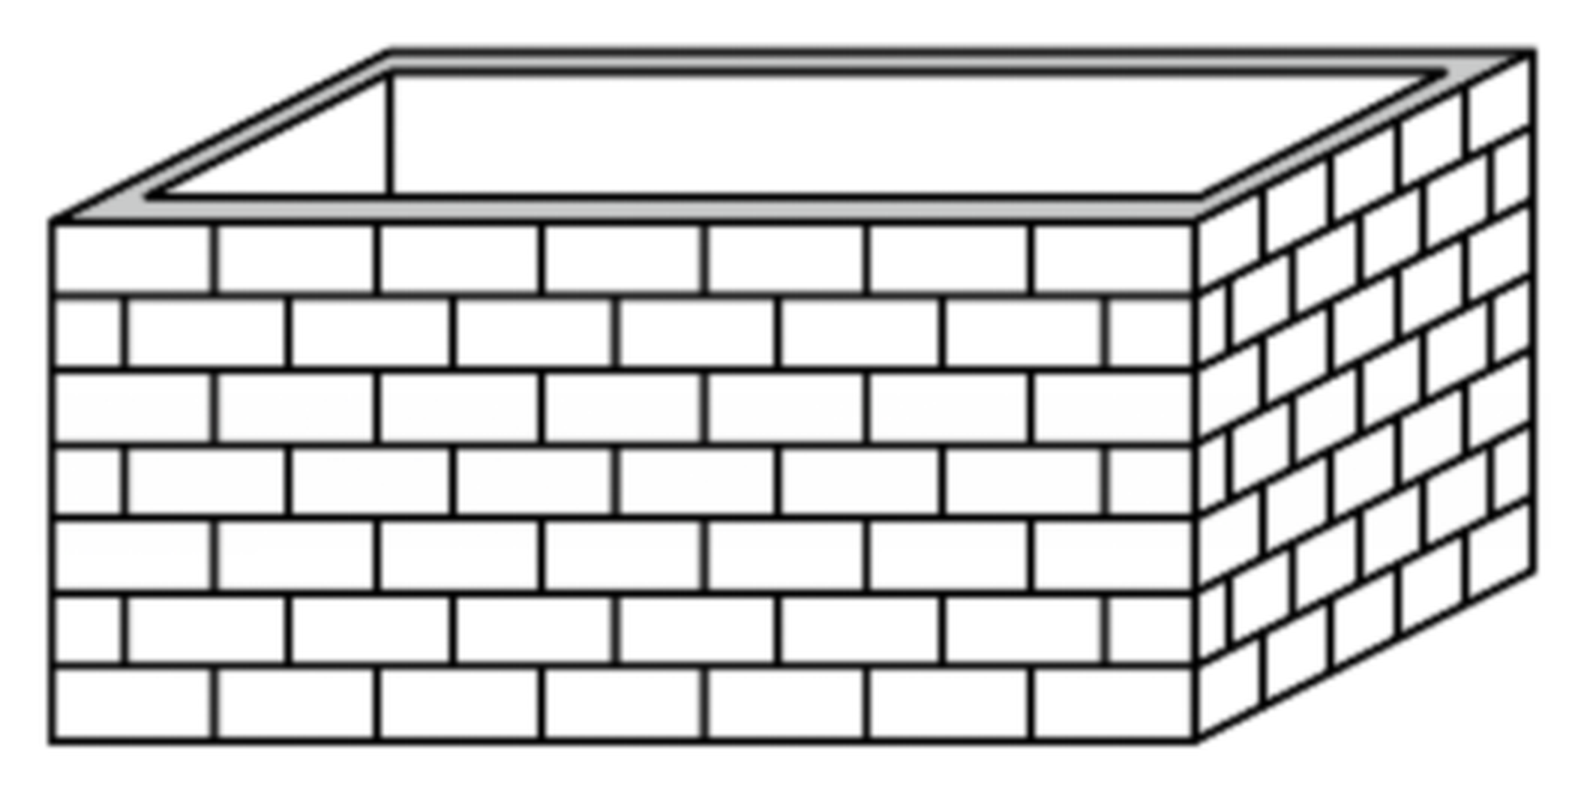
\includegraphics[width=0.42\textwidth]{figures/gao141_q19.png}
\end{center}

\ifanswer
\solbegin
\step{(1) 设水池的长、宽分别为 $xm$，$ym$，则 $x-y\geqslant60$，且 $x$、$y>0$，}
\step{由题意得 $2xy=3200$，即 $x=\dfrac{1600}{y}$，所以 $\dfrac{1600}{y}-y\geqslant60$，}
\step{因为 $y>0$，所以 $1600-y^2\geqslant60y$，}
\step{即 $y^2+60y-1600=(y+80)(y-20)\leqslant0$，解得 $-80\leqslant y\leqslant20$，}
\step{又 $y>0$，所以 $0<y\leqslant20$，所以水池的宽的最大值为 $20m$.}
\step{(2) 设水池总造价为 $z$ 元，}
\step{则 $z=1600\times150+2\times(2x+2y)\times120=240000+480(x+y)$，}
\step{又因为 $y=\dfrac{1600}{x}$，}
\step{所以 $z=240000+\left(x+\dfrac{1600}{x}\right)\times480\geqslant240000+480\times2\sqrt{1600}$}
\step{$=240000+38400=278400$，}
\step{当且仅当 $x=\dfrac{1600}{x}$，即 $x=y=40$ 时取等号，}
\step{所以，将水池的池底设计为边长为 $40m$ 的正方形时总造价最低，}
\step{最低总造价为 $278400$ 元.}
\solend
\fi

\item 已知 $a\in\R$，设集合 $A=\{x\mid ax^2-3x+2<ax-1\}$.

(1) 若 $A=(1,3)$，求实数 $a$ 的值；

(2) 当 $a>0$ 时，求 $A$；

(3) 若 “ $x\in\left(\dfrac12,+\infty\right)$ ” 是 “ $x\in A$ ” 的必要非充分条件，求实数 $a$ 的取值范围.

\ifanswer
\solbegin
\step{原不等式等价于 $ax^2-(a+3)x+3<0\Leftrightarrow(x-1)(ax-3)<0$，}
\step{(1) $A=(1,3)$ 为有界区间，因此 $a>0$，两根为 $1$ 和 $\dfrac3a$，于是 $\dfrac3a=3$，得 $a=1$；}
\step{此时 $(x-1)(x-3)<0$ 的解集确为 $(1,3)$.}
\step{(2) 当 $a>0$ 时，二次项系数为正，比较 $1$ 与 $\dfrac3a$，得 $A=\begin{cases}\left(1,\dfrac3a\right),&0<a<3\\\varnothing,&a=3\\\left(\dfrac3a,1\right),&a>3\end{cases}$，}
\step{其中 $a=3$ 时，原不等式为 $3(x-1)^2<0$，无解.}
\step{(3) 记 $S=\left(\dfrac12,+\infty\right)$，题意要求 $A\subset S$.}% 子集符号原卷印单线 $\subset$，照录
\step{由于对任意 $a$ 都有 $1\notin A$，而 $1\in S$，所以只需满足 $A\subseteq S$.}
\step{当 $a<0$ 时，$A=\left(-\infty,\dfrac3a\right)\cup(1,+\infty)$，含有小于 $\dfrac12$ 的数，不符合条件.}
\step{当 $a=0$ 时，$A=(1,+\infty)$，符合条件.}
\step{当 $0<a<3$ 时，$A=\left(1,\dfrac3a\right)\subseteq S$；}
\step{当 $a=3$ 时，$A=\varnothing\subseteq S$，均符合条件；}
\step{当 $a>3$ 时，$A=\left(\dfrac3a,1\right)$，所以 $A\subseteq S\Leftrightarrow\dfrac3a\geqslant\dfrac12\Leftrightarrow a\leqslant6$；}
\step{因此实数 $a$ 的取值范围为 $[0,6]$.}
\solend
\fi

\item 甲、乙两同学探讨了一个问题：已知正实数 $x,y$ 满足 $3x+y=1$，求 $\dfrac1x+\dfrac1y$ 的最小值.

甲给出的解法：由 $1=3x+y\geqslant2\sqrt{3xy}$，得 $\sqrt{xy}\leqslant\dfrac{\sqrt3}{6}$，所以 $\dfrac1x+\dfrac1y\geqslant2\sqrt{\dfrac1{xy}}\geqslant4\sqrt3$. 因此 $\dfrac1x+\dfrac1y$ 的最小值为 $4\sqrt3$.

乙给出的解法：$\dfrac1x+\dfrac1y=\left(\dfrac1x+\dfrac1y\right)(3x+y)=4+\dfrac yx+\dfrac{3x}{y}$，因为 $x,y$ 均为正实数，所以 $\dfrac1x+\dfrac1y\geqslant4+2\sqrt{\dfrac yx\cdot\dfrac{3x}{y}}=4+2\sqrt3$.

(1) 请判断上述哪位同学的解法正确，哪位同学的解法错误，并指出错误的原因；

(2) 结合上述探讨，试求当 $0<x<\dfrac12$ 时，$\dfrac1x+\dfrac1{1-2x}$ 的最小值以及此时实数 $x$ 的值；

(3) 已知 $x$ 为正实数，$y$ 为非负实数，且 $x+2y=2$，求 $\dfrac{x^2+1}{x}+\dfrac{2y^2}{y+1}$ 的最小值以及此时实数 $x,y$ 的值.

\ifanswer
\solbegin
\step{(1) 甲的推导中，$3x+y\geqslant2\sqrt{3xy}$ 取等号要求 $3x=y$，}
\step{$\dfrac1x+\dfrac1y\geqslant\dfrac2{\sqrt{xy}}$ 取等号要求 $x=y$，两者对正实数 $x,y$ 不能同时成立，}
\step{因此不能将 $4\sqrt3$ 判为最小值，甲错误.}
\step{乙的等号条件为 $\dfrac yx=\dfrac{3x}{y}$，即 $y=\sqrt3 x$；}
\step{结合 $3x+y=1$，得 $x=\dfrac1{3+\sqrt3},y=\dfrac{\sqrt3}{3+\sqrt3}$ 均为正数，等号可以成立，}
\step{因此乙正确，最小值为 $4+2\sqrt3$.}
\step{(2) 令 $t=1-2x>0$，则 $2x+t=1$.}
\step{$\dfrac1x+\dfrac1t=\left(\dfrac1x+\dfrac1t\right)(2x+t)=3+\dfrac tx+\dfrac{2x}{t}\geqslant3+2\sqrt2$，}
\step{当且仅当 $\dfrac tx=\dfrac{2x}{t}$，即 $t=\sqrt2 x$ 时取等号，}
\step{由 $2x+t=1$，得 $x=\dfrac1{2+\sqrt2}=\dfrac{2-\sqrt2}{2}\in\left(0,\dfrac12\right)$，}
\step{因此最小值为 $3+2\sqrt2$，此时 $x=\dfrac{2-\sqrt2}{2}$.}
\step{(3) 记目标式为 $F$，利用 $x+2y=2$，}
\step{得 $F=x+\dfrac1x+2y-2+\dfrac2{y+1}=\dfrac1x+\dfrac2{y+1}$，}
\step{又 $x+2(y+1)=4$，且 $x>0$、$y+1>0$，}
\step{所以 $4F=\left(\dfrac1x+\dfrac2{y+1}\right)(x+2(y+1))=5+2\left(\dfrac{y+1}{x}+\dfrac{x}{y+1}\right)$}
\step{$\geqslant5+2\times2=9$，当且仅当 $\dfrac{y+1}{x}=\dfrac{x}{y+1}$，即 $x=y+1$ 时取等号.}
\step{联立 $x+2y=2$，得 $x=\dfrac43$、$y=\dfrac13$，满足题设条件，}
\step{因此最小值为 $\dfrac94$，此时 $x=\dfrac43$，$y=\dfrac13$.}
\solend
\fi

\end{enumerate}

\end{document}
"
% 紧凑版：xelatex "\def\iscompact{1}% 高一141_彭浦中学_期中.tex
%   —— 高一上数学"2026-2027 年彭浦中学高一上期中"（试卷版/答案版/紧凑版）
% 试卷版：xelatex 高一141_彭浦中学_期中.tex
% 答案版：xelatex "\def\isanswer{1}\input{高一141_彭浦中学_期中.tex}"
% 紧凑版：xelatex "\def\iscompact{1}\input{高一141_彭浦中学_期中.tex}"
%
% ① 原始材料：微信公众号"魔都数学加油站"文章，连载"27学年高一141"，原文标题
% "27学年高一141——2026-2027年上海市彭浦中学高一上期中"；
% 原文链接：https://mp.weixin.qq.com/s/V_8bEhC6geeFyQysmtqUtQ。
% 正文为 9 张 PNG 页（01、05、06、07、09 为 2560x3620；02、03、04、08 为 4762x6735，
% 同一篇各页分辨率不同，逐页按各自分辨率放大裁图核对），题目下印【解析】，为讲评版。
% 题目、解析均据原图转录；卷面粉红色水印"魔都数学加油站"及公众号页脚未录入。
% 全卷 2 幅插图，均属题目配图（在 \ifanswer 外、三版都出）、取原卷截图去粉色水印、
% LANCZOS 放大 3 倍：第 5 题韦恩图（01 页，全集 U 矩形内两圆相交、交集阴影、A/B/U 标注）、
% 第 19 题长方体无盖贮水池砖墙示意图（06 页右上）。通读 9 页确认除这 2 幅外无其它
% 插图/表格，亦无"题干写如图而源码漏图"（仅 Q5"图中阴影部分"、Q19"如图所示"两处提到图）。
%
% 卷首标题：原卷印作"2026-2027 年彭浦中学高一上期中"（公众号标题中的"上海市"
% 卷面标题行没有，本稿照卷面），年份区间按全稿惯例排 en dash；原卷未印副标题，
% 本卷为期中卷、跨集合与常用逻辑用语／不等式／函数三章，按题目内容补出
% "集合与常用逻辑用语、不等式、函数"（与 高一140 同期中卷口径相同）：
% 集合与逻辑见 Q5、Q10、Q12、Q13、Q16、Q17、Q20，不等式见 Q4、Q9、Q14、Q18、
% Q19、Q21，函数（指数／对数）见 Q6、Q15。
%
% 题号体例：本卷共 19 题——一、填空题 3—12（10 题）、二、选择题 13—16（4 题）、
% 三、解答题 17—21（5 题）。三节分别 \setcounter{enumi}{2}／{12}／{16}。
% 原卷从第 3 题起、无第 1、2 题，本稿保留原题号；全卷无附加题节。
%
% ② 与原卷的排版差异：
%   ① 原文从第 3 题起，本稿保留原题号；
%   ② 原卷 19 题题下均印【解析】，无独立【答案】段、无"答案印题干括号且无解析"、
%      无"只印【答案】无解析"一型：填空题与解答题的答案落在【解析】末句
%      （Q3—Q12、Q17—Q21），四道选择题答案在【解析】末句"故选 …"
%      （Q13 选 A、Q14 选 C、Q15 选 D、Q16 选 C），题干括号内一律留空；
%      本稿 19 题一律 \solbegin…\solend、全卷不提 \ans{}，答案版【解析】标记数
%      = 19 = 全卷题数（无【答案】标记）；
%   ③ 原卷未印副标题，本稿按"知识模块"口径补出；
%   ④ 原卷填空横线按全稿惯例排 \blankline[4.4em]；选择题括号排 \mbox{（\quad）}，
%      选项段／命题段前按惯例加 \keepwithprev（Q16 两枚：命题列与选项段各一）；
%      解答题不留作答区、不加 \anspace（原卷为讲评版，与 129／131／132／133／136／140 同）；
%   ⑤ 原卷数集混排：黑板粗体 R（Q14 题干、Q16 ① 与解析、Q17 全集、Q20 题干）
%      按全稿惯例统一改 \R；空集记号 \varnothing；绝对值排 \lvert…\rvert，
%      集合描述竖线排 \mid；不等号按全稿惯例排 \leqslant／\geqslant；
%      补集照原卷上划线排 \overline{A\cap B}（Q17(2) 题干与解析）；
%      原卷"card"记号排黑体正体（Q12），本稿照录 \mathbf{card}，未改斜体
%      （与 高一66 同题口径不同：那份原卷 card 排斜体、照录 $card(M)$）；
%   ⑥ 子题标号 (1)(2)(3) 原卷印半角括号，照录；圈数字 ①②③④ 在正文（文本模式）
%      按原卷照录，未进数学式；数学式内半角逗号照录（如 Q12"$A,B$"、"{1,2,3}"、
%      Q14"$a,b,c\in\R$"、Q15"$\log_{14}7=a$，$14^b=5$"、Q16"$a=1,b=0$"、
%      Q18"$x,y,z$"、Q20"$x,y$"、Q21"$x,y$"）；全卷行末西文句点照录为 ASCII 句点；
%      行中全角逗号、顿号照录；
%   ⑦ 题干中的中文弯引号按原卷照录（Q13、Q20(3) 的 “ ” 及引号内空格），
%      注释内一律 ASCII 引号；
%   ⑧ 两幅题目配图各在 \item 之前加 \needvspace 守卫整块推走（Q5 5cm、Q19 6cm），
%      守卫放在 \item 之前而非 \bigsec 之后——两题均非各节首题，不触发 B 类
%      "节标题落页末"（照 高一26／40／59／136／140 成例）；三版切页审计均"合计异常：无"；
%   ⑨ 跨页续印按题合并：Q8 题干与【解析】首行在 01 页、后 6 行在 02 页；
%      Q15 题干在 03 页、【解析】在 04 页；Q17 题干与【解析】前 2 行在 04 页、
%      后 4 行在 05 页；Q19 题干在 05 页末、(1)(2) 小问与砖墙图与【解析】在 06 页；
%      Q20 题干 (1)(2) 在 06 页末、(3) 与【解析】在 07 页；Q21 题干与【解析】
%      前 6 行在 08 页、后 12 行在 09 页；Q16、Q18 全在各自页内；
%      本稿按题连排，不丢行；
%   ⑩ 原卷无红色加粗标签（【解析】均黑色印刷，Q16 解析 "①取…""④取…" 与
%      Q20 解析 "(2)" 等分步标签亦黑色），故本卷未用 \stepm；
%   ⑪ 原卷 Q19 题干把数值与单位（3200m³、2m、60m、150 元、120 元、40m、20m、
%      278400 元）印作略粗的西文字形，本稿按全稿惯例（高一70／72 同类题）排普通
%      数学体，未加粗。
%
% ③ 行数复核：一条 \step = 原卷解析的一个印刷行，cases 块作一个印刷行计。逐题数 \step
%   条数，合计 92 条（Q3：1；Q4：1；Q5：1；Q6：1；Q7：2；Q8：7；Q9：1；Q10：4；
%   Q11：4；Q12：4；Q13：2；Q14：1；Q15：2；Q16：4；Q17：6；Q18：7；Q19：13；
%   Q20：13；Q21：18），与原卷印刷行逐题相等。全卷 19 题均印【解析】、无独立 \ans{}，
%   答案版【解析】标记数 = 19 = 全卷题数。
%
% ④ 判别式／子集符号结论（逐处放大原图照录、不得统一）：
%   判别式：全卷 3 处——第 7 题【解析】"$\Delta=a^2-4\cdot\frac14=0$"一处原卷印
%     等腰、偏高的高三角 $\Delta$，照录 \Delta；第 8 题【解析】
%     "$\triangle=25-40=-15<0$"与"$\triangle=1+8=9>0$"两处原卷印扁等边三角
%     $\triangle$，照录 \triangle。两形不同，逐处照录未统一。
%   子集：全卷 6 处——第 10 题【解析】"$B\subseteq A$"一处、第 20 题【解析】
%     "所以只需满足 $A\subseteq S$"、"$A=\left(1,\frac3a\right)\subseteq S$"、
%     "$A=\varnothing\subseteq S$"、"$A\subseteq S\Leftrightarrow\frac3a\geqslant\frac12$"
%     四处，共 5 处原卷印带下划线的 $\subseteq$，照录 \subseteq；第 20 题【解析】
%     (3) 首行"题意要求 $A\subset S$"一处原卷印单线 $\subset$，照录 \subset
%     （下行因 $1\in S$ 而 $1\notin A$，改述为 $A\subseteq S$，两者逻辑一致、非笔误）。
%
% ⑤ 存疑照录（照录未改，正文对应处另有 % 注）：
%   第 14 题题干"设 $a,b,c\in\R$"只声明 $a,b,c$，而 A 选项"若 $a>b$ 且 $c>d$，
%     则 $ac>bd$"引入未声明的 $d$，原卷变量声明与选项不统一，照录未补。
%   全卷除此 1 条外未发现其它笔误／自相矛盾处。
%
% ⑥ 跨页续印按题合并说明：见 ② ⑨。
%
\documentclass[a4paper,11pt]{article}
\usepackage{common}

\begin{document}

\examtitlest[3]{2026--2027 年彭浦中学高一上期中}{集合与常用逻辑用语、不等式、函数}

\bigsec{一、填空题}

\begin{enumerate}
\setcounter{enumi}{2}

\item 已知 $m$ 为实数，若 $1\in\{m,m^2\}$，则 $m$ 的值为\blankline[4.4em].

\ifanswer
\solbegin
\step{$m=1$ 或 $m^2=1$，得 $m=\pm1$；按列举项互异口径排除 $m=m^2=1$，得 $m=-1$.}
\solend
\fi

\item 已知 $2<a<4$，$-2<b<1$，则 $2a+b$ 的取值范围为\blankline[4.4em].

\ifanswer
\solbegin
\step{$4<2a<8$，与 $-2<b<1$ 相加，得 $2<2a+b<9$，取值范围为 $(2,9)$.}
\solend
\fi

% 第 5 题韦恩图（题目配图，三版都出）：取原卷 01 页截图去粉色水印、LANCZOS 放大 3 倍
\needvspace{5cm}
\item 已知集合 $A=\{-1,-2,1,4,7\}$，$B=\{x\mid x>1\}$，用列举法表示图中阴影部分所表示的集合为\blankline[4.4em].

\begin{center}
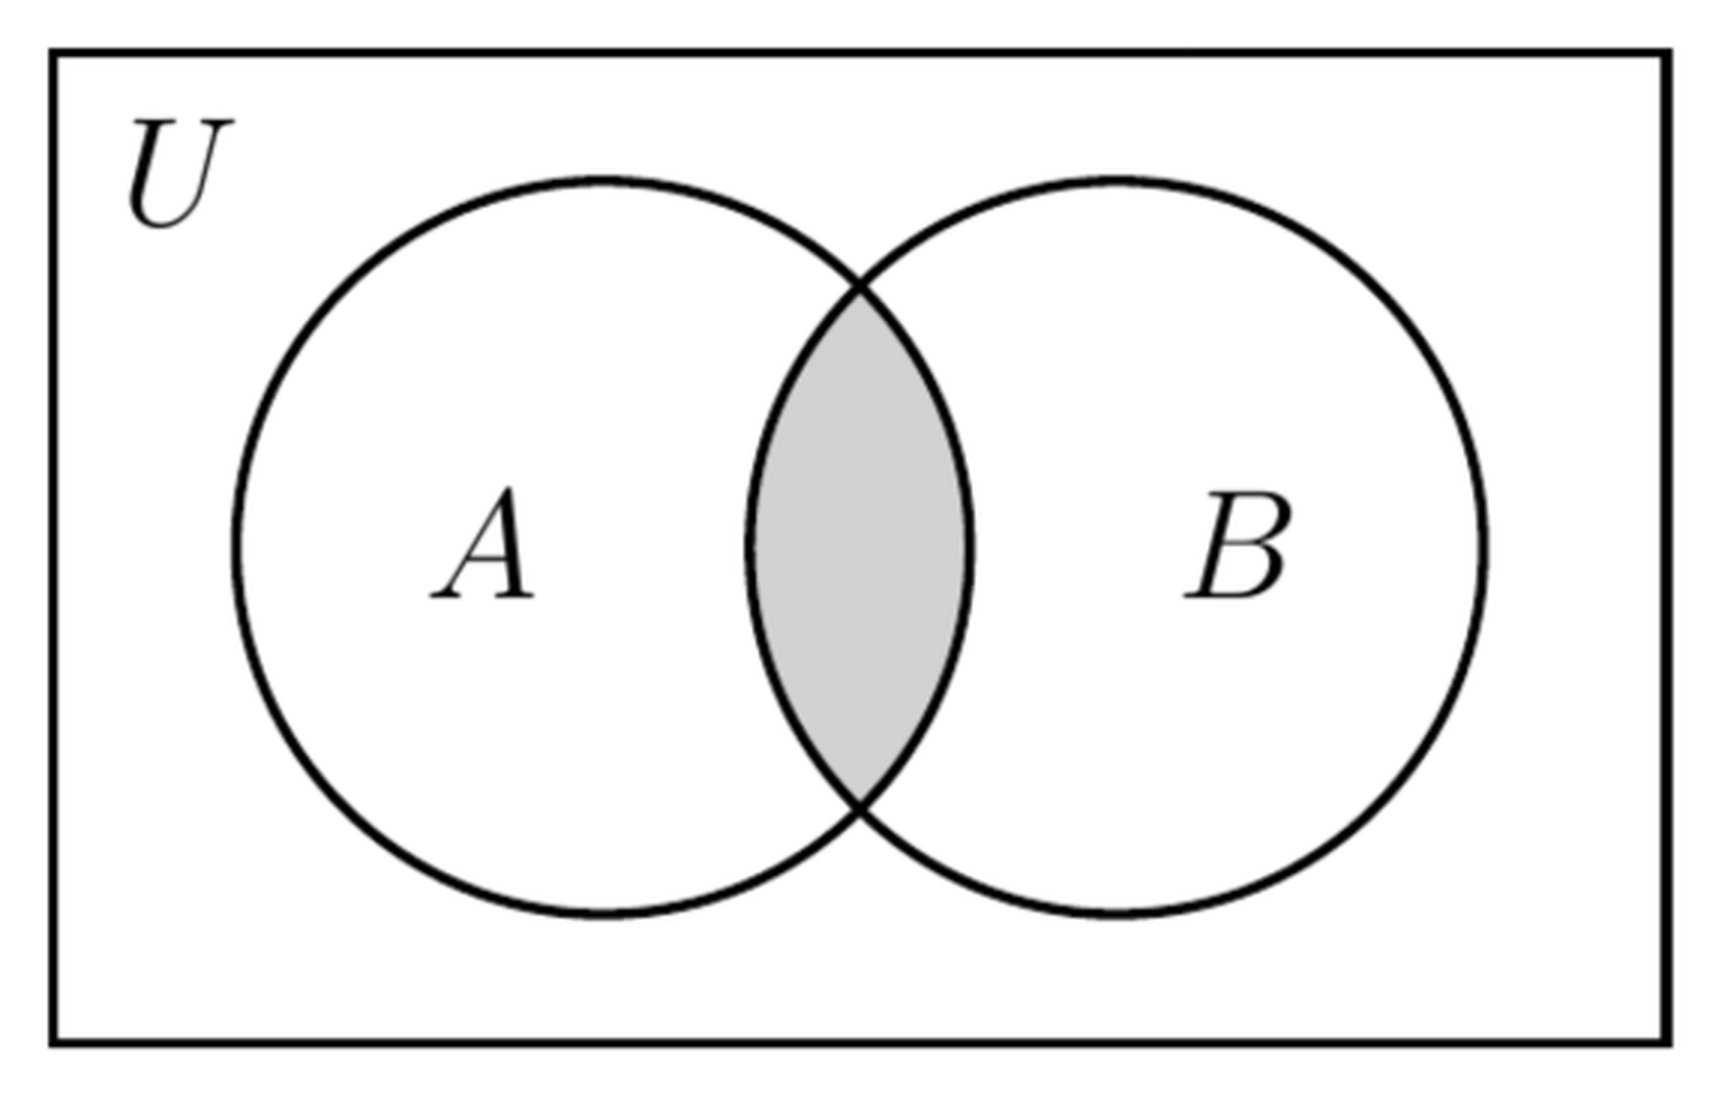
\includegraphics[width=0.38\textwidth]{figures/gao141_q5.png}
\end{center}

\ifanswer
\solbegin
\step{阴影部分表示 $A\cap B=\{4,7\}$.}
\solend
\fi

\item 方程 $2^{\log_3 x}=\dfrac12$ 的解集为\blankline[4.4em].

\ifanswer
\solbegin
\step{$2^{\log_3 x}=2^{-1}\Leftrightarrow\log_3 x=-1\Leftrightarrow x=\dfrac13$，解集为 $\left\{\dfrac13\right\}$.}
\solend
\fi

\item 若集合 $A=\left\{x\mid x^2+ax+\dfrac14=0\right\}$ 有且仅有两个子集，则实数 $a$ 的值为\blankline[4.4em].

\ifanswer
\solbegin
\step{$A$ 有且仅有两个子集，说明 $A$ 恰有一个元素，即方程有两个相等的实数根.}
\step{$\Delta=a^2-4\cdot\dfrac14=0\Rightarrow a=\pm1$.}% 判别式原卷印等腰偏高的高三角 $\Delta$，照录
\solend
\fi

\item 已知关于 $x$ 的方程 $x^2+mx+2m=0$ 的两个实数根分别为 $\alpha$、$\beta$，若 $\alpha^2+\beta^2=5$，则实数 $m=$\blankline[4.4em].

\ifanswer
\solbegin
\step{方程 $x^2+mx+2m=0$ 的两个实数根为 $\alpha$、$\beta$，}
\step{由根与系数的关系得 $\begin{cases}\alpha+\beta=-m\\\alpha\beta=2m\end{cases}$，又因为 $\alpha^2+\beta^2=5$，}
\step{所以 $\alpha^2+\beta^2=(\alpha+\beta)^2-2\alpha\beta=m^2-4m=5$，整理得 $m^2-4m-5=0$，}
\step{解得 $m=5$ 或 $m=-1$，}
\step{当 $m=5$ 时，$\triangle=25-40=-15<0$，无实根，舍去；}% 判别式原卷印扁等边三角 $\triangle$，照录
\step{当 $m=-1$ 时，$\triangle=1+8=9>0$，符合题意，}
\step{所以实数 $m=-1$.}
\solend
\fi

\item 若不等式 $\lvert x-3\rvert+\lvert x-5\rvert\geqslant a$ 对任意的实数 $x$ 恒成立，则实数 $a$ 的取值范围为\blankline[4.4em].

\ifanswer
\solbegin
\step{由三角不等式得 $\lvert x-3\rvert+\lvert x-5\rvert\geqslant\lvert x-3-x+5\rvert=2$，则 $a\leqslant2$.}
\solend
\fi

\item 设集合 $A=\{-3,2\}$，集合 $B=\{x\mid mx+1=0\}$，若 $A\cup B=A$，则实数 $m$ 的值为\blankline[4.4em].

\ifanswer
\solbegin
\step{由 $A\cup B=A$，得 $B\subseteq A$，}% 子集符号原卷印带下划线的 $\subseteq$，照录
\step{当 $m=0$ 时，$B=\varnothing$，满足题意，}
\step{当 $m\neq0$ 时，$B=\left\{-\dfrac1m\right\}$，所以 $-\dfrac1m=2$ 或 $-\dfrac1m=-3$，所以 $m=-\dfrac12$ 或 $m=\dfrac13$，}
\step{综上所述，$m=0$ 或 $m=-\dfrac12$ 或 $m=\dfrac13$.}
\solend
\fi

\item 已知 $m$ 为实数，代数式 $M=\sqrt{m-1}+\sqrt{3-m}$ 的取值范围为\blankline[4.4em].

\ifanswer
\solbegin
\step{根式有意义要求 $m\in[1,3]$，}
\step{此时 $(m-1)(3-m)=1-(m-2)^2$ 的取值范围为 $[0,1]$.}
\step{$M^2=2+2\sqrt{(m-1)(3-m)}$ 的取值范围为 $[2,4]$，又 $M>0$，}
\step{所以 $M\in[\sqrt2,2]$.}
\solend
\fi

\item 设有限集 $M$ 所含元素的个数用 $\mathbf{card}(M)$ 表示，并规定 $\mathbf{card}(\varnothing)=0$. 已知集合 $A,B$ 满足 $A\cup B=\{1,2,3\}$，$A\cap B=\varnothing$，若 $\mathbf{card}(A)\notin A$，$\mathbf{card}(B)\notin B$，则满足条件的所有不同集合 $A$ 的个数为\blankline[4.4em].

\ifanswer
\solbegin
\step{当 $\mathbf{card}(A)=0$ 或 $3$ 时，$A,B$ 中有一个为 $\{1,2,3\}$，不符合条件.}
\step{当 $\mathbf{card}(A)=1$ 时，$\mathbf{card}(B)=2\notin B$，所以 $A=\{2\}$，符合条件.}
\step{当 $\mathbf{card}(A)=2$ 时，$2\notin A$，所以 $B=\{2\}$，$A=\{1,3\}$，符合条件.}
\step{满足条件的集合 $A$ 共 $2$ 个.}
\solend
\fi

\end{enumerate}

\bigsec{二、选择题}

\begin{enumerate}
\setcounter{enumi}{12}

\item “ $x=1$ ” 是 “ $x^2-3x+2=0$ ” 的\mbox{（\quad）}条件.

\keepwithprev
A. 充分非必要\qquad B. 必要非充分

C. 充要\qquad D. 既非充分又非必要

\ifanswer
\solbegin
\step{$x^2-3x+2=0\Leftrightarrow x=1$ 或 $x=2$，所以 “ $x=1$ ” 是其充分非必要条件，}
\step{故选 $A$.}
\solend
\fi

\item 设 $a,b,c\in\R$，则下列命题为真命题的是\mbox{（\quad）}
% 原卷题干只声明 a,b,c，而 A 选项出现未声明的 d，照录（存疑）
\keepwithprev
A. 若 $a>b$ 且 $c>d$，则 $ac>bd$\qquad B. 若 $a^2>b^2$，则 $a>b$

C. 若 $ab>0$ 且 $a>b$，则 $\dfrac1a<\dfrac1b$\qquad D. 若 $a<0<b$，则 $\sqrt{-a}<\sqrt b$

\ifanswer
\solbegin
\step{$ab>0$ 且 $a>b\Rightarrow\dfrac1a-\dfrac1b=\dfrac{b-a}{ab}<0$，所以 $C$ 为真命题，故选 $C$.}
\solend
\fi

\item 已知 $\log_{14}7=a$，$14^b=5$，则 $\log_{35}28=$\mbox{（\quad）}

\keepwithprev
A. $\dfrac{2-a}{2a+b}$\qquad B. $\dfrac{2+a}{a+b}$\qquad C. $\dfrac{2-a}{a+2b}$\qquad D. $\dfrac{2-a}{a+b}$

\ifanswer
\solbegin
\step{$\log_{14}7=a$，$14^b=5$，}
\step{$\log_{35}28=\dfrac{\log_{14}28}{\log_{14}35}=\dfrac{\log_{14}14^2-\log_{14}7}{\log_{14}7+\log_{14}5}=\dfrac{2-a}{a+b}$. 故选 $D$.}
\solend
\fi

\item 关于 $x$ 的不等式 $ax^2+bx+3>0$ 的解集有下列说法，其中正确的个数是\mbox{（\quad）}

\keepwithprev
① 不等式 $ax^2+bx+3>0$ 的解集可以是 $\R$

② 不等式 $ax^2+bx+3>0$ 的解集可以是 $\{x\mid x>3\}$

③ 不等式 $ax^2+bx+3>0$ 的解集可以是 $\varnothing$

④ 不等式 $ax^2+bx+3>0$ 的解集可以是 $\{x\mid -1<x<3\}$

\keepwithprev
A. 4\qquad B. 3\qquad C. 2\qquad D. 1

\ifanswer
\solbegin
\step{$x=0$ 时左端为 $3>0$，解集必含 $0$，所以②③错误.}
\step{①取 $a=1,b=0$，$x^2+3>0$ 的解集为 $\R$，正确.}
\step{④取 $a=-1,b=2$，$-x^2+2x+3=-(x+1)(x-3)>0\Leftrightarrow-1<x<3$，正确.}
\step{正确的有①④，共 $2$ 个，故选 $C$.}
\solend
\fi

\end{enumerate}

\bigsec{三、解答题}

\begin{enumerate}
\setcounter{enumi}{16}

\item 已知集合 $A=\left\{x\mid\dfrac{x-2}{x+3}\geqslant0\right\}$，集合 $B=\{x\mid\lvert x+1\rvert+\lvert x-1\rvert<5\}$，全集 $U=\R$.

(1) 求 $A,B$；

(2) 求 $A\cup B$、$\overline{A\cap B}$.

\ifanswer
\solbegin
\step{(1) 分母不为零，且分子、分母同号或分子为零，}
\step{所以 $\dfrac{x-2}{x+3}\geqslant0\Leftrightarrow x<-3$ 或 $x\geqslant2$，因此 $A=(-\infty,-3)\cup[2,+\infty)$.}
\step{又 $\lvert x+1\rvert+\lvert x-1\rvert=\begin{cases}-2x,&x<-1\\2,&-1\leqslant x\leqslant1\\2x,&x>1\end{cases}$，}
\step{分别解得 $-\dfrac52<x<-1$、$-1\leqslant x\leqslant1$、$1<x<\dfrac52$，因此 $B=\left(-\dfrac52,\dfrac52\right)$.}
\step{(2) 合并两集合所对应的区间，得 $A\cup B=(-\infty,-3)\cup\left(-\dfrac52,+\infty\right)$，}
\step{两集合的公共部分为 $A\cap B=\left[2,\dfrac52\right)$，所以 $\overline{A\cap B}=(-\infty,2)\cup\left[\dfrac52,+\infty\right)$.}
\solend
\fi

\item (1) 已知 $a>b>0$，比较代数式 $\dfrac ab$ 与 $\dfrac{a+1}{b+1}$ 的大小并说明理由；

(2) 已知 $x,y,z$ 都是正实数，$a=x+\dfrac1y,b=y+\dfrac1z,c=z+\dfrac1x$，试用反证法证明 $a,b,c$ 至少有一个不小于 $2$.

\ifanswer
\solbegin
\step{(1) $\dfrac ab-\dfrac{a+1}{b+1}=\dfrac{a(b+1)-b(a+1)}{b(b+1)}=\dfrac{a-b}{b(b+1)}$，}
\step{因为 $a>b>0$，所以 $a-b>0$，$b(b+1)>0$，所以 $\dfrac ab-\dfrac{a+1}{b+1}>0$，}
\step{故 $\dfrac ab>\dfrac{a+1}{b+1}$.}
\step{(2) 假设 $a$、$b$、$c$ 三数都小于 $2$，则 $x+\dfrac1y+y+\dfrac1z+z+\dfrac1x<6$.}
\step{因为 $x,y,z$ 均大于 $0$，}
\step{所以 $x+\dfrac1y+y+\dfrac1z+z+\dfrac1x=x+\dfrac1x+y+\dfrac1y+z+\dfrac1z\geqslant2+2+2=6$，矛盾，}
\step{所以 $a$、$b$、$c$ 三数中至少有一个不小于 $2$.}
\solend
\fi

% 第 19 题长方体无盖贮水池砖墙示意图（题目配图，三版都出）：取原卷 06 页截图去粉色水印、LANCZOS 放大 3 倍
\needvspace{6cm}
\item 如图所示，某工厂要建造一个长方体形无盖贮水池，其容积为 $3200m^3$，深为 $2m$.

(1) 若水池的长比宽至少多 $60m$，求水池的宽的最大值；

(2) 若池底每平方米的造价为 $150$ 元，池壁每平方米的造价为 $120$ 元，那么怎样设计水池的长和宽能使总造价最低？最低总造价是多少？

\begin{center}
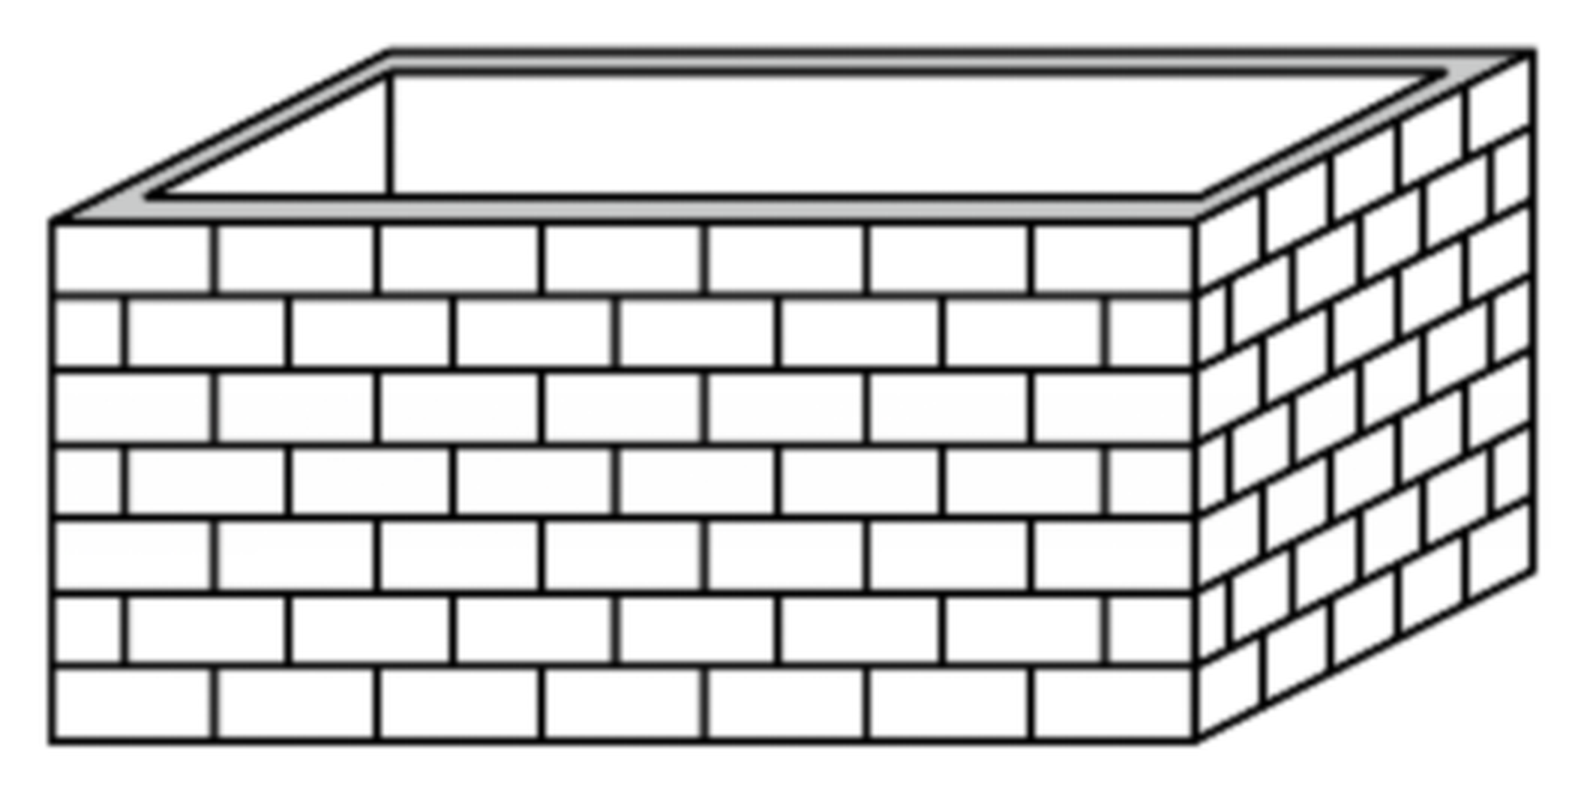
\includegraphics[width=0.42\textwidth]{figures/gao141_q19.png}
\end{center}

\ifanswer
\solbegin
\step{(1) 设水池的长、宽分别为 $xm$，$ym$，则 $x-y\geqslant60$，且 $x$、$y>0$，}
\step{由题意得 $2xy=3200$，即 $x=\dfrac{1600}{y}$，所以 $\dfrac{1600}{y}-y\geqslant60$，}
\step{因为 $y>0$，所以 $1600-y^2\geqslant60y$，}
\step{即 $y^2+60y-1600=(y+80)(y-20)\leqslant0$，解得 $-80\leqslant y\leqslant20$，}
\step{又 $y>0$，所以 $0<y\leqslant20$，所以水池的宽的最大值为 $20m$.}
\step{(2) 设水池总造价为 $z$ 元，}
\step{则 $z=1600\times150+2\times(2x+2y)\times120=240000+480(x+y)$，}
\step{又因为 $y=\dfrac{1600}{x}$，}
\step{所以 $z=240000+\left(x+\dfrac{1600}{x}\right)\times480\geqslant240000+480\times2\sqrt{1600}$}
\step{$=240000+38400=278400$，}
\step{当且仅当 $x=\dfrac{1600}{x}$，即 $x=y=40$ 时取等号，}
\step{所以，将水池的池底设计为边长为 $40m$ 的正方形时总造价最低，}
\step{最低总造价为 $278400$ 元.}
\solend
\fi

\item 已知 $a\in\R$，设集合 $A=\{x\mid ax^2-3x+2<ax-1\}$.

(1) 若 $A=(1,3)$，求实数 $a$ 的值；

(2) 当 $a>0$ 时，求 $A$；

(3) 若 “ $x\in\left(\dfrac12,+\infty\right)$ ” 是 “ $x\in A$ ” 的必要非充分条件，求实数 $a$ 的取值范围.

\ifanswer
\solbegin
\step{原不等式等价于 $ax^2-(a+3)x+3<0\Leftrightarrow(x-1)(ax-3)<0$，}
\step{(1) $A=(1,3)$ 为有界区间，因此 $a>0$，两根为 $1$ 和 $\dfrac3a$，于是 $\dfrac3a=3$，得 $a=1$；}
\step{此时 $(x-1)(x-3)<0$ 的解集确为 $(1,3)$.}
\step{(2) 当 $a>0$ 时，二次项系数为正，比较 $1$ 与 $\dfrac3a$，得 $A=\begin{cases}\left(1,\dfrac3a\right),&0<a<3\\\varnothing,&a=3\\\left(\dfrac3a,1\right),&a>3\end{cases}$，}
\step{其中 $a=3$ 时，原不等式为 $3(x-1)^2<0$，无解.}
\step{(3) 记 $S=\left(\dfrac12,+\infty\right)$，题意要求 $A\subset S$.}% 子集符号原卷印单线 $\subset$，照录
\step{由于对任意 $a$ 都有 $1\notin A$，而 $1\in S$，所以只需满足 $A\subseteq S$.}
\step{当 $a<0$ 时，$A=\left(-\infty,\dfrac3a\right)\cup(1,+\infty)$，含有小于 $\dfrac12$ 的数，不符合条件.}
\step{当 $a=0$ 时，$A=(1,+\infty)$，符合条件.}
\step{当 $0<a<3$ 时，$A=\left(1,\dfrac3a\right)\subseteq S$；}
\step{当 $a=3$ 时，$A=\varnothing\subseteq S$，均符合条件；}
\step{当 $a>3$ 时，$A=\left(\dfrac3a,1\right)$，所以 $A\subseteq S\Leftrightarrow\dfrac3a\geqslant\dfrac12\Leftrightarrow a\leqslant6$；}
\step{因此实数 $a$ 的取值范围为 $[0,6]$.}
\solend
\fi

\item 甲、乙两同学探讨了一个问题：已知正实数 $x,y$ 满足 $3x+y=1$，求 $\dfrac1x+\dfrac1y$ 的最小值.

甲给出的解法：由 $1=3x+y\geqslant2\sqrt{3xy}$，得 $\sqrt{xy}\leqslant\dfrac{\sqrt3}{6}$，所以 $\dfrac1x+\dfrac1y\geqslant2\sqrt{\dfrac1{xy}}\geqslant4\sqrt3$. 因此 $\dfrac1x+\dfrac1y$ 的最小值为 $4\sqrt3$.

乙给出的解法：$\dfrac1x+\dfrac1y=\left(\dfrac1x+\dfrac1y\right)(3x+y)=4+\dfrac yx+\dfrac{3x}{y}$，因为 $x,y$ 均为正实数，所以 $\dfrac1x+\dfrac1y\geqslant4+2\sqrt{\dfrac yx\cdot\dfrac{3x}{y}}=4+2\sqrt3$.

(1) 请判断上述哪位同学的解法正确，哪位同学的解法错误，并指出错误的原因；

(2) 结合上述探讨，试求当 $0<x<\dfrac12$ 时，$\dfrac1x+\dfrac1{1-2x}$ 的最小值以及此时实数 $x$ 的值；

(3) 已知 $x$ 为正实数，$y$ 为非负实数，且 $x+2y=2$，求 $\dfrac{x^2+1}{x}+\dfrac{2y^2}{y+1}$ 的最小值以及此时实数 $x,y$ 的值.

\ifanswer
\solbegin
\step{(1) 甲的推导中，$3x+y\geqslant2\sqrt{3xy}$ 取等号要求 $3x=y$，}
\step{$\dfrac1x+\dfrac1y\geqslant\dfrac2{\sqrt{xy}}$ 取等号要求 $x=y$，两者对正实数 $x,y$ 不能同时成立，}
\step{因此不能将 $4\sqrt3$ 判为最小值，甲错误.}
\step{乙的等号条件为 $\dfrac yx=\dfrac{3x}{y}$，即 $y=\sqrt3 x$；}
\step{结合 $3x+y=1$，得 $x=\dfrac1{3+\sqrt3},y=\dfrac{\sqrt3}{3+\sqrt3}$ 均为正数，等号可以成立，}
\step{因此乙正确，最小值为 $4+2\sqrt3$.}
\step{(2) 令 $t=1-2x>0$，则 $2x+t=1$.}
\step{$\dfrac1x+\dfrac1t=\left(\dfrac1x+\dfrac1t\right)(2x+t)=3+\dfrac tx+\dfrac{2x}{t}\geqslant3+2\sqrt2$，}
\step{当且仅当 $\dfrac tx=\dfrac{2x}{t}$，即 $t=\sqrt2 x$ 时取等号，}
\step{由 $2x+t=1$，得 $x=\dfrac1{2+\sqrt2}=\dfrac{2-\sqrt2}{2}\in\left(0,\dfrac12\right)$，}
\step{因此最小值为 $3+2\sqrt2$，此时 $x=\dfrac{2-\sqrt2}{2}$.}
\step{(3) 记目标式为 $F$，利用 $x+2y=2$，}
\step{得 $F=x+\dfrac1x+2y-2+\dfrac2{y+1}=\dfrac1x+\dfrac2{y+1}$，}
\step{又 $x+2(y+1)=4$，且 $x>0$、$y+1>0$，}
\step{所以 $4F=\left(\dfrac1x+\dfrac2{y+1}\right)(x+2(y+1))=5+2\left(\dfrac{y+1}{x}+\dfrac{x}{y+1}\right)$}
\step{$\geqslant5+2\times2=9$，当且仅当 $\dfrac{y+1}{x}=\dfrac{x}{y+1}$，即 $x=y+1$ 时取等号.}
\step{联立 $x+2y=2$，得 $x=\dfrac43$、$y=\dfrac13$，满足题设条件，}
\step{因此最小值为 $\dfrac94$，此时 $x=\dfrac43$，$y=\dfrac13$.}
\solend
\fi

\end{enumerate}

\end{document}
"
%
% ① 原始材料：微信公众号"魔都数学加油站"文章，连载"27学年高一141"，原文标题
% "27学年高一141——2026-2027年上海市彭浦中学高一上期中"；
% 原文链接：https://mp.weixin.qq.com/s/V_8bEhC6geeFyQysmtqUtQ。
% 正文为 9 张 PNG 页（01、05、06、07、09 为 2560x3620；02、03、04、08 为 4762x6735，
% 同一篇各页分辨率不同，逐页按各自分辨率放大裁图核对），题目下印【解析】，为讲评版。
% 题目、解析均据原图转录；卷面粉红色水印"魔都数学加油站"及公众号页脚未录入。
% 全卷 2 幅插图，均属题目配图（在 \ifanswer 外、三版都出）、取原卷截图去粉色水印、
% LANCZOS 放大 3 倍：第 5 题韦恩图（01 页，全集 U 矩形内两圆相交、交集阴影、A/B/U 标注）、
% 第 19 题长方体无盖贮水池砖墙示意图（06 页右上）。通读 9 页确认除这 2 幅外无其它
% 插图/表格，亦无"题干写如图而源码漏图"（仅 Q5"图中阴影部分"、Q19"如图所示"两处提到图）。
%
% 卷首标题：原卷印作"2026-2027 年彭浦中学高一上期中"（公众号标题中的"上海市"
% 卷面标题行没有，本稿照卷面），年份区间按全稿惯例排 en dash；原卷未印副标题，
% 本卷为期中卷、跨集合与常用逻辑用语／不等式／函数三章，按题目内容补出
% "集合与常用逻辑用语、不等式、函数"（与 高一140 同期中卷口径相同）：
% 集合与逻辑见 Q5、Q10、Q12、Q13、Q16、Q17、Q20，不等式见 Q4、Q9、Q14、Q18、
% Q19、Q21，函数（指数／对数）见 Q6、Q15。
%
% 题号体例：本卷共 19 题——一、填空题 3—12（10 题）、二、选择题 13—16（4 题）、
% 三、解答题 17—21（5 题）。三节分别 \setcounter{enumi}{2}／{12}／{16}。
% 原卷从第 3 题起、无第 1、2 题，本稿保留原题号；全卷无附加题节。
%
% ② 与原卷的排版差异：
%   ① 原文从第 3 题起，本稿保留原题号；
%   ② 原卷 19 题题下均印【解析】，无独立【答案】段、无"答案印题干括号且无解析"、
%      无"只印【答案】无解析"一型：填空题与解答题的答案落在【解析】末句
%      （Q3—Q12、Q17—Q21），四道选择题答案在【解析】末句"故选 …"
%      （Q13 选 A、Q14 选 C、Q15 选 D、Q16 选 C），题干括号内一律留空；
%      本稿 19 题一律 \solbegin…\solend、全卷不提 \ans{}，答案版【解析】标记数
%      = 19 = 全卷题数（无【答案】标记）；
%   ③ 原卷未印副标题，本稿按"知识模块"口径补出；
%   ④ 原卷填空横线按全稿惯例排 \blankline[4.4em]；选择题括号排 \mbox{（\quad）}，
%      选项段／命题段前按惯例加 \keepwithprev（Q16 两枚：命题列与选项段各一）；
%      解答题不留作答区、不加 \anspace（原卷为讲评版，与 129／131／132／133／136／140 同）；
%   ⑤ 原卷数集混排：黑板粗体 R（Q14 题干、Q16 ① 与解析、Q17 全集、Q20 题干）
%      按全稿惯例统一改 \R；空集记号 \varnothing；绝对值排 \lvert…\rvert，
%      集合描述竖线排 \mid；不等号按全稿惯例排 \leqslant／\geqslant；
%      补集照原卷上划线排 \overline{A\cap B}（Q17(2) 题干与解析）；
%      原卷"card"记号排黑体正体（Q12），本稿照录 \mathbf{card}，未改斜体
%      （与 高一66 同题口径不同：那份原卷 card 排斜体、照录 $card(M)$）；
%   ⑥ 子题标号 (1)(2)(3) 原卷印半角括号，照录；圈数字 ①②③④ 在正文（文本模式）
%      按原卷照录，未进数学式；数学式内半角逗号照录（如 Q12"$A,B$"、"{1,2,3}"、
%      Q14"$a,b,c\in\R$"、Q15"$\log_{14}7=a$，$14^b=5$"、Q16"$a=1,b=0$"、
%      Q18"$x,y,z$"、Q20"$x,y$"、Q21"$x,y$"）；全卷行末西文句点照录为 ASCII 句点；
%      行中全角逗号、顿号照录；
%   ⑦ 题干中的中文弯引号按原卷照录（Q13、Q20(3) 的 “ ” 及引号内空格），
%      注释内一律 ASCII 引号；
%   ⑧ 两幅题目配图各在 \item 之前加 \needvspace 守卫整块推走（Q5 5cm、Q19 6cm），
%      守卫放在 \item 之前而非 \bigsec 之后——两题均非各节首题，不触发 B 类
%      "节标题落页末"（照 高一26／40／59／136／140 成例）；三版切页审计均"合计异常：无"；
%   ⑨ 跨页续印按题合并：Q8 题干与【解析】首行在 01 页、后 6 行在 02 页；
%      Q15 题干在 03 页、【解析】在 04 页；Q17 题干与【解析】前 2 行在 04 页、
%      后 4 行在 05 页；Q19 题干在 05 页末、(1)(2) 小问与砖墙图与【解析】在 06 页；
%      Q20 题干 (1)(2) 在 06 页末、(3) 与【解析】在 07 页；Q21 题干与【解析】
%      前 6 行在 08 页、后 12 行在 09 页；Q16、Q18 全在各自页内；
%      本稿按题连排，不丢行；
%   ⑩ 原卷无红色加粗标签（【解析】均黑色印刷，Q16 解析 "①取…""④取…" 与
%      Q20 解析 "(2)" 等分步标签亦黑色），故本卷未用 \stepm；
%   ⑪ 原卷 Q19 题干把数值与单位（3200m³、2m、60m、150 元、120 元、40m、20m、
%      278400 元）印作略粗的西文字形，本稿按全稿惯例（高一70／72 同类题）排普通
%      数学体，未加粗。
%
% ③ 行数复核：一条 \step = 原卷解析的一个印刷行，cases 块作一个印刷行计。逐题数 \step
%   条数，合计 92 条（Q3：1；Q4：1；Q5：1；Q6：1；Q7：2；Q8：7；Q9：1；Q10：4；
%   Q11：4；Q12：4；Q13：2；Q14：1；Q15：2；Q16：4；Q17：6；Q18：7；Q19：13；
%   Q20：13；Q21：18），与原卷印刷行逐题相等。全卷 19 题均印【解析】、无独立 \ans{}，
%   答案版【解析】标记数 = 19 = 全卷题数。
%
% ④ 判别式／子集符号结论（逐处放大原图照录、不得统一）：
%   判别式：全卷 3 处——第 7 题【解析】"$\Delta=a^2-4\cdot\frac14=0$"一处原卷印
%     等腰、偏高的高三角 $\Delta$，照录 \Delta；第 8 题【解析】
%     "$\triangle=25-40=-15<0$"与"$\triangle=1+8=9>0$"两处原卷印扁等边三角
%     $\triangle$，照录 \triangle。两形不同，逐处照录未统一。
%   子集：全卷 6 处——第 10 题【解析】"$B\subseteq A$"一处、第 20 题【解析】
%     "所以只需满足 $A\subseteq S$"、"$A=\left(1,\frac3a\right)\subseteq S$"、
%     "$A=\varnothing\subseteq S$"、"$A\subseteq S\Leftrightarrow\frac3a\geqslant\frac12$"
%     四处，共 5 处原卷印带下划线的 $\subseteq$，照录 \subseteq；第 20 题【解析】
%     (3) 首行"题意要求 $A\subset S$"一处原卷印单线 $\subset$，照录 \subset
%     （下行因 $1\in S$ 而 $1\notin A$，改述为 $A\subseteq S$，两者逻辑一致、非笔误）。
%
% ⑤ 存疑照录（照录未改，正文对应处另有 % 注）：
%   第 14 题题干"设 $a,b,c\in\R$"只声明 $a,b,c$，而 A 选项"若 $a>b$ 且 $c>d$，
%     则 $ac>bd$"引入未声明的 $d$，原卷变量声明与选项不统一，照录未补。
%   全卷除此 1 条外未发现其它笔误／自相矛盾处。
%
% ⑥ 跨页续印按题合并说明：见 ② ⑨。
%
\documentclass[a4paper,11pt]{article}
\usepackage{common}

\begin{document}

\examtitlest[3]{2026--2027 年彭浦中学高一上期中}{集合与常用逻辑用语、不等式、函数}

\bigsec{一、填空题}

\begin{enumerate}
\setcounter{enumi}{2}

\item 已知 $m$ 为实数，若 $1\in\{m,m^2\}$，则 $m$ 的值为\blankline[4.4em].

\ifanswer
\solbegin
\step{$m=1$ 或 $m^2=1$，得 $m=\pm1$；按列举项互异口径排除 $m=m^2=1$，得 $m=-1$.}
\solend
\fi

\item 已知 $2<a<4$，$-2<b<1$，则 $2a+b$ 的取值范围为\blankline[4.4em].

\ifanswer
\solbegin
\step{$4<2a<8$，与 $-2<b<1$ 相加，得 $2<2a+b<9$，取值范围为 $(2,9)$.}
\solend
\fi

% 第 5 题韦恩图（题目配图，三版都出）：取原卷 01 页截图去粉色水印、LANCZOS 放大 3 倍
\needvspace{5cm}
\item 已知集合 $A=\{-1,-2,1,4,7\}$，$B=\{x\mid x>1\}$，用列举法表示图中阴影部分所表示的集合为\blankline[4.4em].

\begin{center}
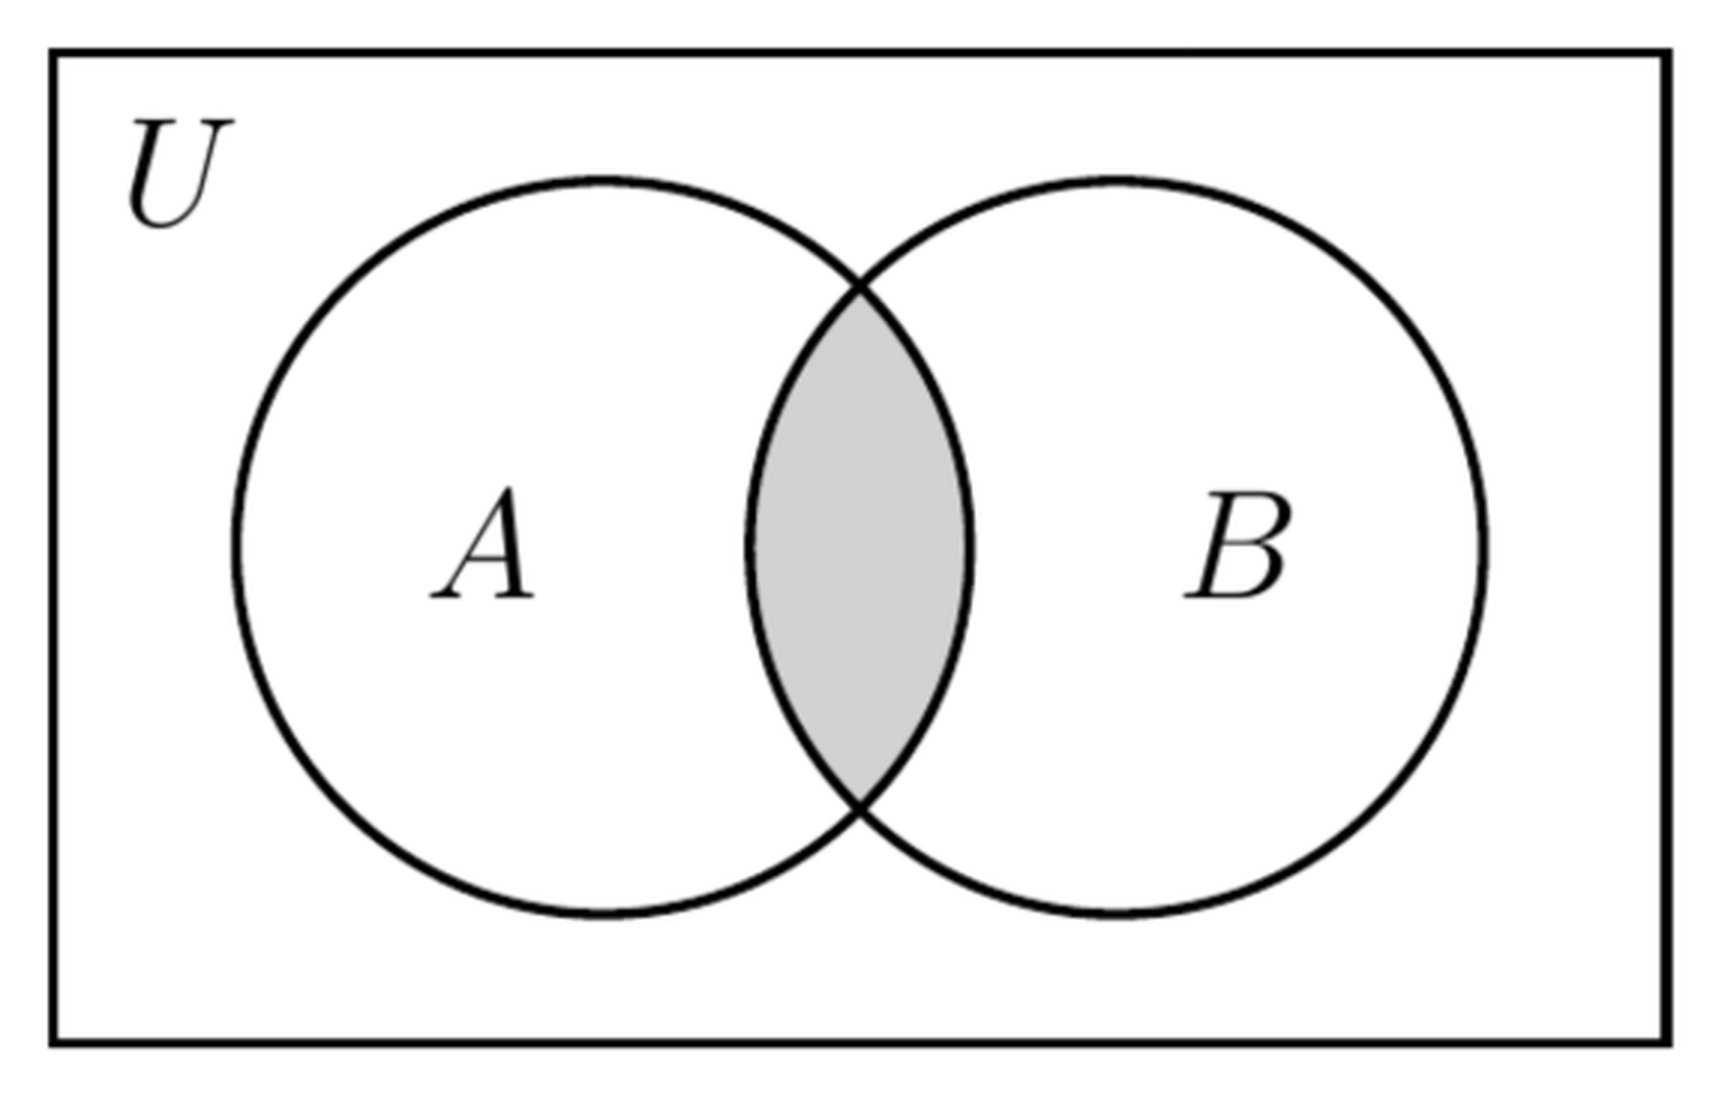
\includegraphics[width=0.38\textwidth]{figures/gao141_q5.png}
\end{center}

\ifanswer
\solbegin
\step{阴影部分表示 $A\cap B=\{4,7\}$.}
\solend
\fi

\item 方程 $2^{\log_3 x}=\dfrac12$ 的解集为\blankline[4.4em].

\ifanswer
\solbegin
\step{$2^{\log_3 x}=2^{-1}\Leftrightarrow\log_3 x=-1\Leftrightarrow x=\dfrac13$，解集为 $\left\{\dfrac13\right\}$.}
\solend
\fi

\item 若集合 $A=\left\{x\mid x^2+ax+\dfrac14=0\right\}$ 有且仅有两个子集，则实数 $a$ 的值为\blankline[4.4em].

\ifanswer
\solbegin
\step{$A$ 有且仅有两个子集，说明 $A$ 恰有一个元素，即方程有两个相等的实数根.}
\step{$\Delta=a^2-4\cdot\dfrac14=0\Rightarrow a=\pm1$.}% 判别式原卷印等腰偏高的高三角 $\Delta$，照录
\solend
\fi

\item 已知关于 $x$ 的方程 $x^2+mx+2m=0$ 的两个实数根分别为 $\alpha$、$\beta$，若 $\alpha^2+\beta^2=5$，则实数 $m=$\blankline[4.4em].

\ifanswer
\solbegin
\step{方程 $x^2+mx+2m=0$ 的两个实数根为 $\alpha$、$\beta$，}
\step{由根与系数的关系得 $\begin{cases}\alpha+\beta=-m\\\alpha\beta=2m\end{cases}$，又因为 $\alpha^2+\beta^2=5$，}
\step{所以 $\alpha^2+\beta^2=(\alpha+\beta)^2-2\alpha\beta=m^2-4m=5$，整理得 $m^2-4m-5=0$，}
\step{解得 $m=5$ 或 $m=-1$，}
\step{当 $m=5$ 时，$\triangle=25-40=-15<0$，无实根，舍去；}% 判别式原卷印扁等边三角 $\triangle$，照录
\step{当 $m=-1$ 时，$\triangle=1+8=9>0$，符合题意，}
\step{所以实数 $m=-1$.}
\solend
\fi

\item 若不等式 $\lvert x-3\rvert+\lvert x-5\rvert\geqslant a$ 对任意的实数 $x$ 恒成立，则实数 $a$ 的取值范围为\blankline[4.4em].

\ifanswer
\solbegin
\step{由三角不等式得 $\lvert x-3\rvert+\lvert x-5\rvert\geqslant\lvert x-3-x+5\rvert=2$，则 $a\leqslant2$.}
\solend
\fi

\item 设集合 $A=\{-3,2\}$，集合 $B=\{x\mid mx+1=0\}$，若 $A\cup B=A$，则实数 $m$ 的值为\blankline[4.4em].

\ifanswer
\solbegin
\step{由 $A\cup B=A$，得 $B\subseteq A$，}% 子集符号原卷印带下划线的 $\subseteq$，照录
\step{当 $m=0$ 时，$B=\varnothing$，满足题意，}
\step{当 $m\neq0$ 时，$B=\left\{-\dfrac1m\right\}$，所以 $-\dfrac1m=2$ 或 $-\dfrac1m=-3$，所以 $m=-\dfrac12$ 或 $m=\dfrac13$，}
\step{综上所述，$m=0$ 或 $m=-\dfrac12$ 或 $m=\dfrac13$.}
\solend
\fi

\item 已知 $m$ 为实数，代数式 $M=\sqrt{m-1}+\sqrt{3-m}$ 的取值范围为\blankline[4.4em].

\ifanswer
\solbegin
\step{根式有意义要求 $m\in[1,3]$，}
\step{此时 $(m-1)(3-m)=1-(m-2)^2$ 的取值范围为 $[0,1]$.}
\step{$M^2=2+2\sqrt{(m-1)(3-m)}$ 的取值范围为 $[2,4]$，又 $M>0$，}
\step{所以 $M\in[\sqrt2,2]$.}
\solend
\fi

\item 设有限集 $M$ 所含元素的个数用 $\mathbf{card}(M)$ 表示，并规定 $\mathbf{card}(\varnothing)=0$. 已知集合 $A,B$ 满足 $A\cup B=\{1,2,3\}$，$A\cap B=\varnothing$，若 $\mathbf{card}(A)\notin A$，$\mathbf{card}(B)\notin B$，则满足条件的所有不同集合 $A$ 的个数为\blankline[4.4em].

\ifanswer
\solbegin
\step{当 $\mathbf{card}(A)=0$ 或 $3$ 时，$A,B$ 中有一个为 $\{1,2,3\}$，不符合条件.}
\step{当 $\mathbf{card}(A)=1$ 时，$\mathbf{card}(B)=2\notin B$，所以 $A=\{2\}$，符合条件.}
\step{当 $\mathbf{card}(A)=2$ 时，$2\notin A$，所以 $B=\{2\}$，$A=\{1,3\}$，符合条件.}
\step{满足条件的集合 $A$ 共 $2$ 个.}
\solend
\fi

\end{enumerate}

\bigsec{二、选择题}

\begin{enumerate}
\setcounter{enumi}{12}

\item “ $x=1$ ” 是 “ $x^2-3x+2=0$ ” 的\mbox{（\quad）}条件.

\keepwithprev
A. 充分非必要\qquad B. 必要非充分

C. 充要\qquad D. 既非充分又非必要

\ifanswer
\solbegin
\step{$x^2-3x+2=0\Leftrightarrow x=1$ 或 $x=2$，所以 “ $x=1$ ” 是其充分非必要条件，}
\step{故选 $A$.}
\solend
\fi

\item 设 $a,b,c\in\R$，则下列命题为真命题的是\mbox{（\quad）}
% 原卷题干只声明 a,b,c，而 A 选项出现未声明的 d，照录（存疑）
\keepwithprev
A. 若 $a>b$ 且 $c>d$，则 $ac>bd$\qquad B. 若 $a^2>b^2$，则 $a>b$

C. 若 $ab>0$ 且 $a>b$，则 $\dfrac1a<\dfrac1b$\qquad D. 若 $a<0<b$，则 $\sqrt{-a}<\sqrt b$

\ifanswer
\solbegin
\step{$ab>0$ 且 $a>b\Rightarrow\dfrac1a-\dfrac1b=\dfrac{b-a}{ab}<0$，所以 $C$ 为真命题，故选 $C$.}
\solend
\fi

\item 已知 $\log_{14}7=a$，$14^b=5$，则 $\log_{35}28=$\mbox{（\quad）}

\keepwithprev
A. $\dfrac{2-a}{2a+b}$\qquad B. $\dfrac{2+a}{a+b}$\qquad C. $\dfrac{2-a}{a+2b}$\qquad D. $\dfrac{2-a}{a+b}$

\ifanswer
\solbegin
\step{$\log_{14}7=a$，$14^b=5$，}
\step{$\log_{35}28=\dfrac{\log_{14}28}{\log_{14}35}=\dfrac{\log_{14}14^2-\log_{14}7}{\log_{14}7+\log_{14}5}=\dfrac{2-a}{a+b}$. 故选 $D$.}
\solend
\fi

\item 关于 $x$ 的不等式 $ax^2+bx+3>0$ 的解集有下列说法，其中正确的个数是\mbox{（\quad）}

\keepwithprev
① 不等式 $ax^2+bx+3>0$ 的解集可以是 $\R$

② 不等式 $ax^2+bx+3>0$ 的解集可以是 $\{x\mid x>3\}$

③ 不等式 $ax^2+bx+3>0$ 的解集可以是 $\varnothing$

④ 不等式 $ax^2+bx+3>0$ 的解集可以是 $\{x\mid -1<x<3\}$

\keepwithprev
A. 4\qquad B. 3\qquad C. 2\qquad D. 1

\ifanswer
\solbegin
\step{$x=0$ 时左端为 $3>0$，解集必含 $0$，所以②③错误.}
\step{①取 $a=1,b=0$，$x^2+3>0$ 的解集为 $\R$，正确.}
\step{④取 $a=-1,b=2$，$-x^2+2x+3=-(x+1)(x-3)>0\Leftrightarrow-1<x<3$，正确.}
\step{正确的有①④，共 $2$ 个，故选 $C$.}
\solend
\fi

\end{enumerate}

\bigsec{三、解答题}

\begin{enumerate}
\setcounter{enumi}{16}

\item 已知集合 $A=\left\{x\mid\dfrac{x-2}{x+3}\geqslant0\right\}$，集合 $B=\{x\mid\lvert x+1\rvert+\lvert x-1\rvert<5\}$，全集 $U=\R$.

(1) 求 $A,B$；

(2) 求 $A\cup B$、$\overline{A\cap B}$.

\ifanswer
\solbegin
\step{(1) 分母不为零，且分子、分母同号或分子为零，}
\step{所以 $\dfrac{x-2}{x+3}\geqslant0\Leftrightarrow x<-3$ 或 $x\geqslant2$，因此 $A=(-\infty,-3)\cup[2,+\infty)$.}
\step{又 $\lvert x+1\rvert+\lvert x-1\rvert=\begin{cases}-2x,&x<-1\\2,&-1\leqslant x\leqslant1\\2x,&x>1\end{cases}$，}
\step{分别解得 $-\dfrac52<x<-1$、$-1\leqslant x\leqslant1$、$1<x<\dfrac52$，因此 $B=\left(-\dfrac52,\dfrac52\right)$.}
\step{(2) 合并两集合所对应的区间，得 $A\cup B=(-\infty,-3)\cup\left(-\dfrac52,+\infty\right)$，}
\step{两集合的公共部分为 $A\cap B=\left[2,\dfrac52\right)$，所以 $\overline{A\cap B}=(-\infty,2)\cup\left[\dfrac52,+\infty\right)$.}
\solend
\fi

\item (1) 已知 $a>b>0$，比较代数式 $\dfrac ab$ 与 $\dfrac{a+1}{b+1}$ 的大小并说明理由；

(2) 已知 $x,y,z$ 都是正实数，$a=x+\dfrac1y,b=y+\dfrac1z,c=z+\dfrac1x$，试用反证法证明 $a,b,c$ 至少有一个不小于 $2$.

\ifanswer
\solbegin
\step{(1) $\dfrac ab-\dfrac{a+1}{b+1}=\dfrac{a(b+1)-b(a+1)}{b(b+1)}=\dfrac{a-b}{b(b+1)}$，}
\step{因为 $a>b>0$，所以 $a-b>0$，$b(b+1)>0$，所以 $\dfrac ab-\dfrac{a+1}{b+1}>0$，}
\step{故 $\dfrac ab>\dfrac{a+1}{b+1}$.}
\step{(2) 假设 $a$、$b$、$c$ 三数都小于 $2$，则 $x+\dfrac1y+y+\dfrac1z+z+\dfrac1x<6$.}
\step{因为 $x,y,z$ 均大于 $0$，}
\step{所以 $x+\dfrac1y+y+\dfrac1z+z+\dfrac1x=x+\dfrac1x+y+\dfrac1y+z+\dfrac1z\geqslant2+2+2=6$，矛盾，}
\step{所以 $a$、$b$、$c$ 三数中至少有一个不小于 $2$.}
\solend
\fi

% 第 19 题长方体无盖贮水池砖墙示意图（题目配图，三版都出）：取原卷 06 页截图去粉色水印、LANCZOS 放大 3 倍
\needvspace{6cm}
\item 如图所示，某工厂要建造一个长方体形无盖贮水池，其容积为 $3200m^3$，深为 $2m$.

(1) 若水池的长比宽至少多 $60m$，求水池的宽的最大值；

(2) 若池底每平方米的造价为 $150$ 元，池壁每平方米的造价为 $120$ 元，那么怎样设计水池的长和宽能使总造价最低？最低总造价是多少？

\begin{center}
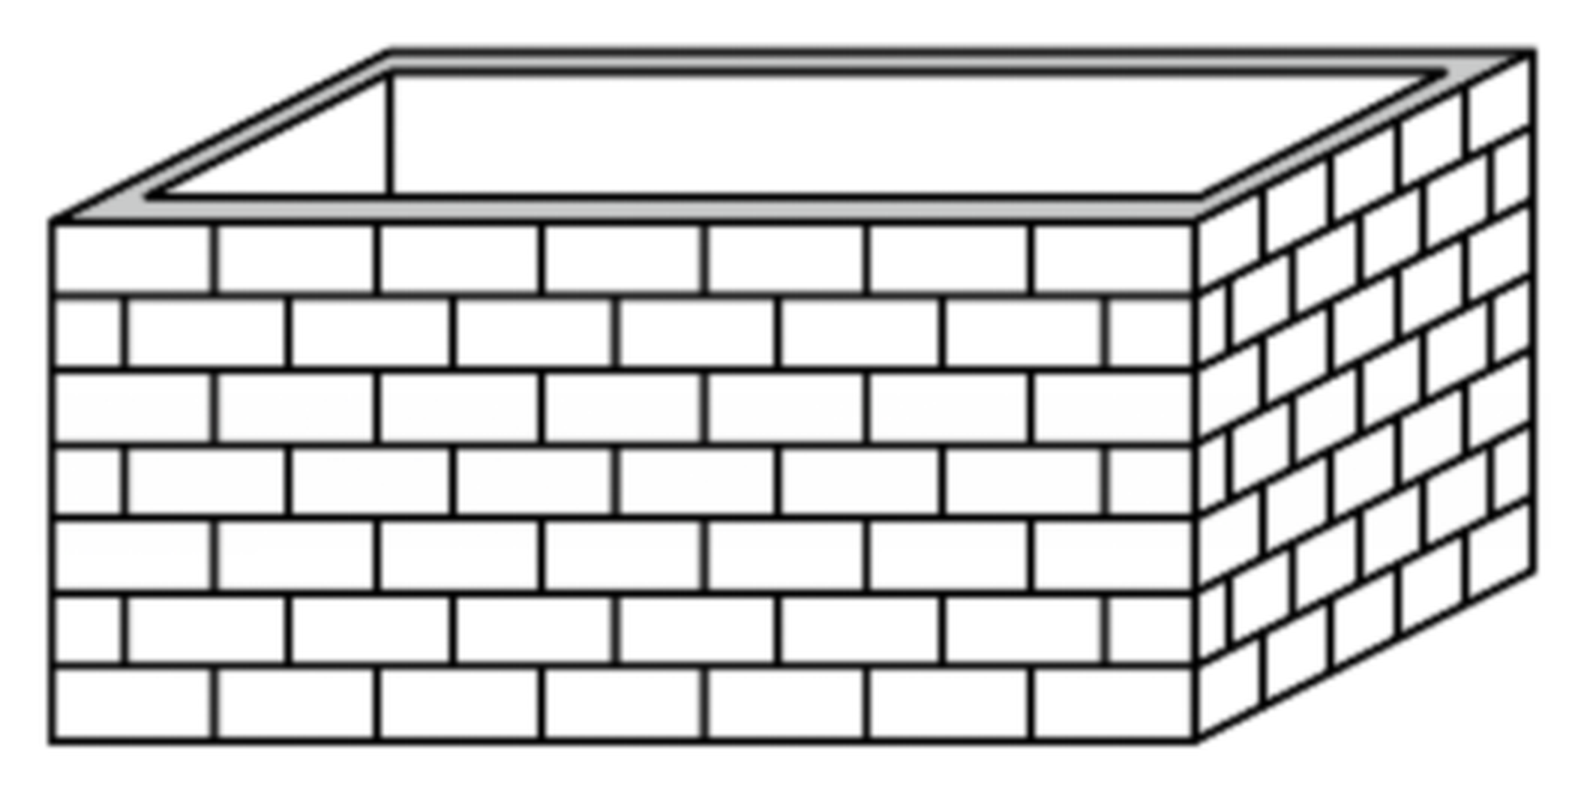
\includegraphics[width=0.42\textwidth]{figures/gao141_q19.png}
\end{center}

\ifanswer
\solbegin
\step{(1) 设水池的长、宽分别为 $xm$，$ym$，则 $x-y\geqslant60$，且 $x$、$y>0$，}
\step{由题意得 $2xy=3200$，即 $x=\dfrac{1600}{y}$，所以 $\dfrac{1600}{y}-y\geqslant60$，}
\step{因为 $y>0$，所以 $1600-y^2\geqslant60y$，}
\step{即 $y^2+60y-1600=(y+80)(y-20)\leqslant0$，解得 $-80\leqslant y\leqslant20$，}
\step{又 $y>0$，所以 $0<y\leqslant20$，所以水池的宽的最大值为 $20m$.}
\step{(2) 设水池总造价为 $z$ 元，}
\step{则 $z=1600\times150+2\times(2x+2y)\times120=240000+480(x+y)$，}
\step{又因为 $y=\dfrac{1600}{x}$，}
\step{所以 $z=240000+\left(x+\dfrac{1600}{x}\right)\times480\geqslant240000+480\times2\sqrt{1600}$}
\step{$=240000+38400=278400$，}
\step{当且仅当 $x=\dfrac{1600}{x}$，即 $x=y=40$ 时取等号，}
\step{所以，将水池的池底设计为边长为 $40m$ 的正方形时总造价最低，}
\step{最低总造价为 $278400$ 元.}
\solend
\fi

\item 已知 $a\in\R$，设集合 $A=\{x\mid ax^2-3x+2<ax-1\}$.

(1) 若 $A=(1,3)$，求实数 $a$ 的值；

(2) 当 $a>0$ 时，求 $A$；

(3) 若 “ $x\in\left(\dfrac12,+\infty\right)$ ” 是 “ $x\in A$ ” 的必要非充分条件，求实数 $a$ 的取值范围.

\ifanswer
\solbegin
\step{原不等式等价于 $ax^2-(a+3)x+3<0\Leftrightarrow(x-1)(ax-3)<0$，}
\step{(1) $A=(1,3)$ 为有界区间，因此 $a>0$，两根为 $1$ 和 $\dfrac3a$，于是 $\dfrac3a=3$，得 $a=1$；}
\step{此时 $(x-1)(x-3)<0$ 的解集确为 $(1,3)$.}
\step{(2) 当 $a>0$ 时，二次项系数为正，比较 $1$ 与 $\dfrac3a$，得 $A=\begin{cases}\left(1,\dfrac3a\right),&0<a<3\\\varnothing,&a=3\\\left(\dfrac3a,1\right),&a>3\end{cases}$，}
\step{其中 $a=3$ 时，原不等式为 $3(x-1)^2<0$，无解.}
\step{(3) 记 $S=\left(\dfrac12,+\infty\right)$，题意要求 $A\subset S$.}% 子集符号原卷印单线 $\subset$，照录
\step{由于对任意 $a$ 都有 $1\notin A$，而 $1\in S$，所以只需满足 $A\subseteq S$.}
\step{当 $a<0$ 时，$A=\left(-\infty,\dfrac3a\right)\cup(1,+\infty)$，含有小于 $\dfrac12$ 的数，不符合条件.}
\step{当 $a=0$ 时，$A=(1,+\infty)$，符合条件.}
\step{当 $0<a<3$ 时，$A=\left(1,\dfrac3a\right)\subseteq S$；}
\step{当 $a=3$ 时，$A=\varnothing\subseteq S$，均符合条件；}
\step{当 $a>3$ 时，$A=\left(\dfrac3a,1\right)$，所以 $A\subseteq S\Leftrightarrow\dfrac3a\geqslant\dfrac12\Leftrightarrow a\leqslant6$；}
\step{因此实数 $a$ 的取值范围为 $[0,6]$.}
\solend
\fi

\item 甲、乙两同学探讨了一个问题：已知正实数 $x,y$ 满足 $3x+y=1$，求 $\dfrac1x+\dfrac1y$ 的最小值.

甲给出的解法：由 $1=3x+y\geqslant2\sqrt{3xy}$，得 $\sqrt{xy}\leqslant\dfrac{\sqrt3}{6}$，所以 $\dfrac1x+\dfrac1y\geqslant2\sqrt{\dfrac1{xy}}\geqslant4\sqrt3$. 因此 $\dfrac1x+\dfrac1y$ 的最小值为 $4\sqrt3$.

乙给出的解法：$\dfrac1x+\dfrac1y=\left(\dfrac1x+\dfrac1y\right)(3x+y)=4+\dfrac yx+\dfrac{3x}{y}$，因为 $x,y$ 均为正实数，所以 $\dfrac1x+\dfrac1y\geqslant4+2\sqrt{\dfrac yx\cdot\dfrac{3x}{y}}=4+2\sqrt3$.

(1) 请判断上述哪位同学的解法正确，哪位同学的解法错误，并指出错误的原因；

(2) 结合上述探讨，试求当 $0<x<\dfrac12$ 时，$\dfrac1x+\dfrac1{1-2x}$ 的最小值以及此时实数 $x$ 的值；

(3) 已知 $x$ 为正实数，$y$ 为非负实数，且 $x+2y=2$，求 $\dfrac{x^2+1}{x}+\dfrac{2y^2}{y+1}$ 的最小值以及此时实数 $x,y$ 的值.

\ifanswer
\solbegin
\step{(1) 甲的推导中，$3x+y\geqslant2\sqrt{3xy}$ 取等号要求 $3x=y$，}
\step{$\dfrac1x+\dfrac1y\geqslant\dfrac2{\sqrt{xy}}$ 取等号要求 $x=y$，两者对正实数 $x,y$ 不能同时成立，}
\step{因此不能将 $4\sqrt3$ 判为最小值，甲错误.}
\step{乙的等号条件为 $\dfrac yx=\dfrac{3x}{y}$，即 $y=\sqrt3 x$；}
\step{结合 $3x+y=1$，得 $x=\dfrac1{3+\sqrt3},y=\dfrac{\sqrt3}{3+\sqrt3}$ 均为正数，等号可以成立，}
\step{因此乙正确，最小值为 $4+2\sqrt3$.}
\step{(2) 令 $t=1-2x>0$，则 $2x+t=1$.}
\step{$\dfrac1x+\dfrac1t=\left(\dfrac1x+\dfrac1t\right)(2x+t)=3+\dfrac tx+\dfrac{2x}{t}\geqslant3+2\sqrt2$，}
\step{当且仅当 $\dfrac tx=\dfrac{2x}{t}$，即 $t=\sqrt2 x$ 时取等号，}
\step{由 $2x+t=1$，得 $x=\dfrac1{2+\sqrt2}=\dfrac{2-\sqrt2}{2}\in\left(0,\dfrac12\right)$，}
\step{因此最小值为 $3+2\sqrt2$，此时 $x=\dfrac{2-\sqrt2}{2}$.}
\step{(3) 记目标式为 $F$，利用 $x+2y=2$，}
\step{得 $F=x+\dfrac1x+2y-2+\dfrac2{y+1}=\dfrac1x+\dfrac2{y+1}$，}
\step{又 $x+2(y+1)=4$，且 $x>0$、$y+1>0$，}
\step{所以 $4F=\left(\dfrac1x+\dfrac2{y+1}\right)(x+2(y+1))=5+2\left(\dfrac{y+1}{x}+\dfrac{x}{y+1}\right)$}
\step{$\geqslant5+2\times2=9$，当且仅当 $\dfrac{y+1}{x}=\dfrac{x}{y+1}$，即 $x=y+1$ 时取等号.}
\step{联立 $x+2y=2$，得 $x=\dfrac43$、$y=\dfrac13$，满足题设条件，}
\step{因此最小值为 $\dfrac94$，此时 $x=\dfrac43$，$y=\dfrac13$.}
\solend
\fi

\end{enumerate}

\end{document}
"
%
% ① 原始材料：微信公众号"魔都数学加油站"文章，连载"27学年高一141"，原文标题
% "27学年高一141——2026-2027年上海市彭浦中学高一上期中"；
% 原文链接：https://mp.weixin.qq.com/s/V_8bEhC6geeFyQysmtqUtQ。
% 正文为 9 张 PNG 页（01、05、06、07、09 为 2560x3620；02、03、04、08 为 4762x6735，
% 同一篇各页分辨率不同，逐页按各自分辨率放大裁图核对），题目下印【解析】，为讲评版。
% 题目、解析均据原图转录；卷面粉红色水印"魔都数学加油站"及公众号页脚未录入。
% 全卷 2 幅插图，均属题目配图（在 \ifanswer 外、三版都出）、取原卷截图去粉色水印、
% LANCZOS 放大 3 倍：第 5 题韦恩图（01 页，全集 U 矩形内两圆相交、交集阴影、A/B/U 标注）、
% 第 19 题长方体无盖贮水池砖墙示意图（06 页右上）。通读 9 页确认除这 2 幅外无其它
% 插图/表格，亦无"题干写如图而源码漏图"（仅 Q5"图中阴影部分"、Q19"如图所示"两处提到图）。
%
% 卷首标题：原卷印作"2026-2027 年彭浦中学高一上期中"（公众号标题中的"上海市"
% 卷面标题行没有，本稿照卷面），年份区间按全稿惯例排 en dash；原卷未印副标题，
% 本卷为期中卷、跨集合与常用逻辑用语／不等式／函数三章，按题目内容补出
% "集合与常用逻辑用语、不等式、函数"（与 高一140 同期中卷口径相同）：
% 集合与逻辑见 Q5、Q10、Q12、Q13、Q16、Q17、Q20，不等式见 Q4、Q9、Q14、Q18、
% Q19、Q21，函数（指数／对数）见 Q6、Q15。
%
% 题号体例：本卷共 19 题——一、填空题 3—12（10 题）、二、选择题 13—16（4 题）、
% 三、解答题 17—21（5 题）。三节分别 \setcounter{enumi}{2}／{12}／{16}。
% 原卷从第 3 题起、无第 1、2 题，本稿保留原题号；全卷无附加题节。
%
% ② 与原卷的排版差异：
%   ① 原文从第 3 题起，本稿保留原题号；
%   ② 原卷 19 题题下均印【解析】，无独立【答案】段、无"答案印题干括号且无解析"、
%      无"只印【答案】无解析"一型：填空题与解答题的答案落在【解析】末句
%      （Q3—Q12、Q17—Q21），四道选择题答案在【解析】末句"故选 …"
%      （Q13 选 A、Q14 选 C、Q15 选 D、Q16 选 C），题干括号内一律留空；
%      本稿 19 题一律 \solbegin…\solend、全卷不提 \ans{}，答案版【解析】标记数
%      = 19 = 全卷题数（无【答案】标记）；
%   ③ 原卷未印副标题，本稿按"知识模块"口径补出；
%   ④ 原卷填空横线按全稿惯例排 \blankline[4.4em]；选择题括号排 \mbox{（\quad）}，
%      选项段／命题段前按惯例加 \keepwithprev（Q16 两枚：命题列与选项段各一）；
%      解答题不留作答区、不加 \anspace（原卷为讲评版，与 129／131／132／133／136／140 同）；
%   ⑤ 原卷数集混排：黑板粗体 R（Q14 题干、Q16 ① 与解析、Q17 全集、Q20 题干）
%      按全稿惯例统一改 \R；空集记号 \varnothing；绝对值排 \lvert…\rvert，
%      集合描述竖线排 \mid；不等号按全稿惯例排 \leqslant／\geqslant；
%      补集照原卷上划线排 \overline{A\cap B}（Q17(2) 题干与解析）；
%      原卷"card"记号排黑体正体（Q12），本稿照录 \mathbf{card}，未改斜体
%      （与 高一66 同题口径不同：那份原卷 card 排斜体、照录 $card(M)$）；
%   ⑥ 子题标号 (1)(2)(3) 原卷印半角括号，照录；圈数字 ①②③④ 在正文（文本模式）
%      按原卷照录，未进数学式；数学式内半角逗号照录（如 Q12"$A,B$"、"{1,2,3}"、
%      Q14"$a,b,c\in\R$"、Q15"$\log_{14}7=a$，$14^b=5$"、Q16"$a=1,b=0$"、
%      Q18"$x,y,z$"、Q20"$x,y$"、Q21"$x,y$"）；全卷行末西文句点照录为 ASCII 句点；
%      行中全角逗号、顿号照录；
%   ⑦ 题干中的中文弯引号按原卷照录（Q13、Q20(3) 的 “ ” 及引号内空格），
%      注释内一律 ASCII 引号；
%   ⑧ 两幅题目配图各在 \item 之前加 \needvspace 守卫整块推走（Q5 5cm、Q19 6cm），
%      守卫放在 \item 之前而非 \bigsec 之后——两题均非各节首题，不触发 B 类
%      "节标题落页末"（照 高一26／40／59／136／140 成例）；三版切页审计均"合计异常：无"；
%   ⑨ 跨页续印按题合并：Q8 题干与【解析】首行在 01 页、后 6 行在 02 页；
%      Q15 题干在 03 页、【解析】在 04 页；Q17 题干与【解析】前 2 行在 04 页、
%      后 4 行在 05 页；Q19 题干在 05 页末、(1)(2) 小问与砖墙图与【解析】在 06 页；
%      Q20 题干 (1)(2) 在 06 页末、(3) 与【解析】在 07 页；Q21 题干与【解析】
%      前 6 行在 08 页、后 12 行在 09 页；Q16、Q18 全在各自页内；
%      本稿按题连排，不丢行；
%   ⑩ 原卷无红色加粗标签（【解析】均黑色印刷，Q16 解析 "①取…""④取…" 与
%      Q20 解析 "(2)" 等分步标签亦黑色），故本卷未用 \stepm；
%   ⑪ 原卷 Q19 题干把数值与单位（3200m³、2m、60m、150 元、120 元、40m、20m、
%      278400 元）印作略粗的西文字形，本稿按全稿惯例（高一70／72 同类题）排普通
%      数学体，未加粗。
%
% ③ 行数复核：一条 \step = 原卷解析的一个印刷行，cases 块作一个印刷行计。逐题数 \step
%   条数，合计 92 条（Q3：1；Q4：1；Q5：1；Q6：1；Q7：2；Q8：7；Q9：1；Q10：4；
%   Q11：4；Q12：4；Q13：2；Q14：1；Q15：2；Q16：4；Q17：6；Q18：7；Q19：13；
%   Q20：13；Q21：18），与原卷印刷行逐题相等。全卷 19 题均印【解析】、无独立 \ans{}，
%   答案版【解析】标记数 = 19 = 全卷题数。
%
% ④ 判别式／子集符号结论（逐处放大原图照录、不得统一）：
%   判别式：全卷 3 处——第 7 题【解析】"$\Delta=a^2-4\cdot\frac14=0$"一处原卷印
%     等腰、偏高的高三角 $\Delta$，照录 \Delta；第 8 题【解析】
%     "$\triangle=25-40=-15<0$"与"$\triangle=1+8=9>0$"两处原卷印扁等边三角
%     $\triangle$，照录 \triangle。两形不同，逐处照录未统一。
%   子集：全卷 6 处——第 10 题【解析】"$B\subseteq A$"一处、第 20 题【解析】
%     "所以只需满足 $A\subseteq S$"、"$A=\left(1,\frac3a\right)\subseteq S$"、
%     "$A=\varnothing\subseteq S$"、"$A\subseteq S\Leftrightarrow\frac3a\geqslant\frac12$"
%     四处，共 5 处原卷印带下划线的 $\subseteq$，照录 \subseteq；第 20 题【解析】
%     (3) 首行"题意要求 $A\subset S$"一处原卷印单线 $\subset$，照录 \subset
%     （下行因 $1\in S$ 而 $1\notin A$，改述为 $A\subseteq S$，两者逻辑一致、非笔误）。
%
% ⑤ 存疑照录（照录未改，正文对应处另有 % 注）：
%   第 14 题题干"设 $a,b,c\in\R$"只声明 $a,b,c$，而 A 选项"若 $a>b$ 且 $c>d$，
%     则 $ac>bd$"引入未声明的 $d$，原卷变量声明与选项不统一，照录未补。
%   全卷除此 1 条外未发现其它笔误／自相矛盾处。
%
% ⑥ 跨页续印按题合并说明：见 ② ⑨。
%
\documentclass[a4paper,11pt]{article}
\usepackage{common}

\begin{document}

\examtitlest[3]{2026--2027 年彭浦中学高一上期中}{集合与常用逻辑用语、不等式、函数}

\bigsec{一、填空题}

\begin{enumerate}
\setcounter{enumi}{2}

\item 已知 $m$ 为实数，若 $1\in\{m,m^2\}$，则 $m$ 的值为\blankline[4.4em].

\ifanswer
\solbegin
\step{$m=1$ 或 $m^2=1$，得 $m=\pm1$；按列举项互异口径排除 $m=m^2=1$，得 $m=-1$.}
\solend
\fi

\item 已知 $2<a<4$，$-2<b<1$，则 $2a+b$ 的取值范围为\blankline[4.4em].

\ifanswer
\solbegin
\step{$4<2a<8$，与 $-2<b<1$ 相加，得 $2<2a+b<9$，取值范围为 $(2,9)$.}
\solend
\fi

% 第 5 题韦恩图（题目配图，三版都出）：取原卷 01 页截图去粉色水印、LANCZOS 放大 3 倍
\needvspace{5cm}
\item 已知集合 $A=\{-1,-2,1,4,7\}$，$B=\{x\mid x>1\}$，用列举法表示图中阴影部分所表示的集合为\blankline[4.4em].

\begin{center}
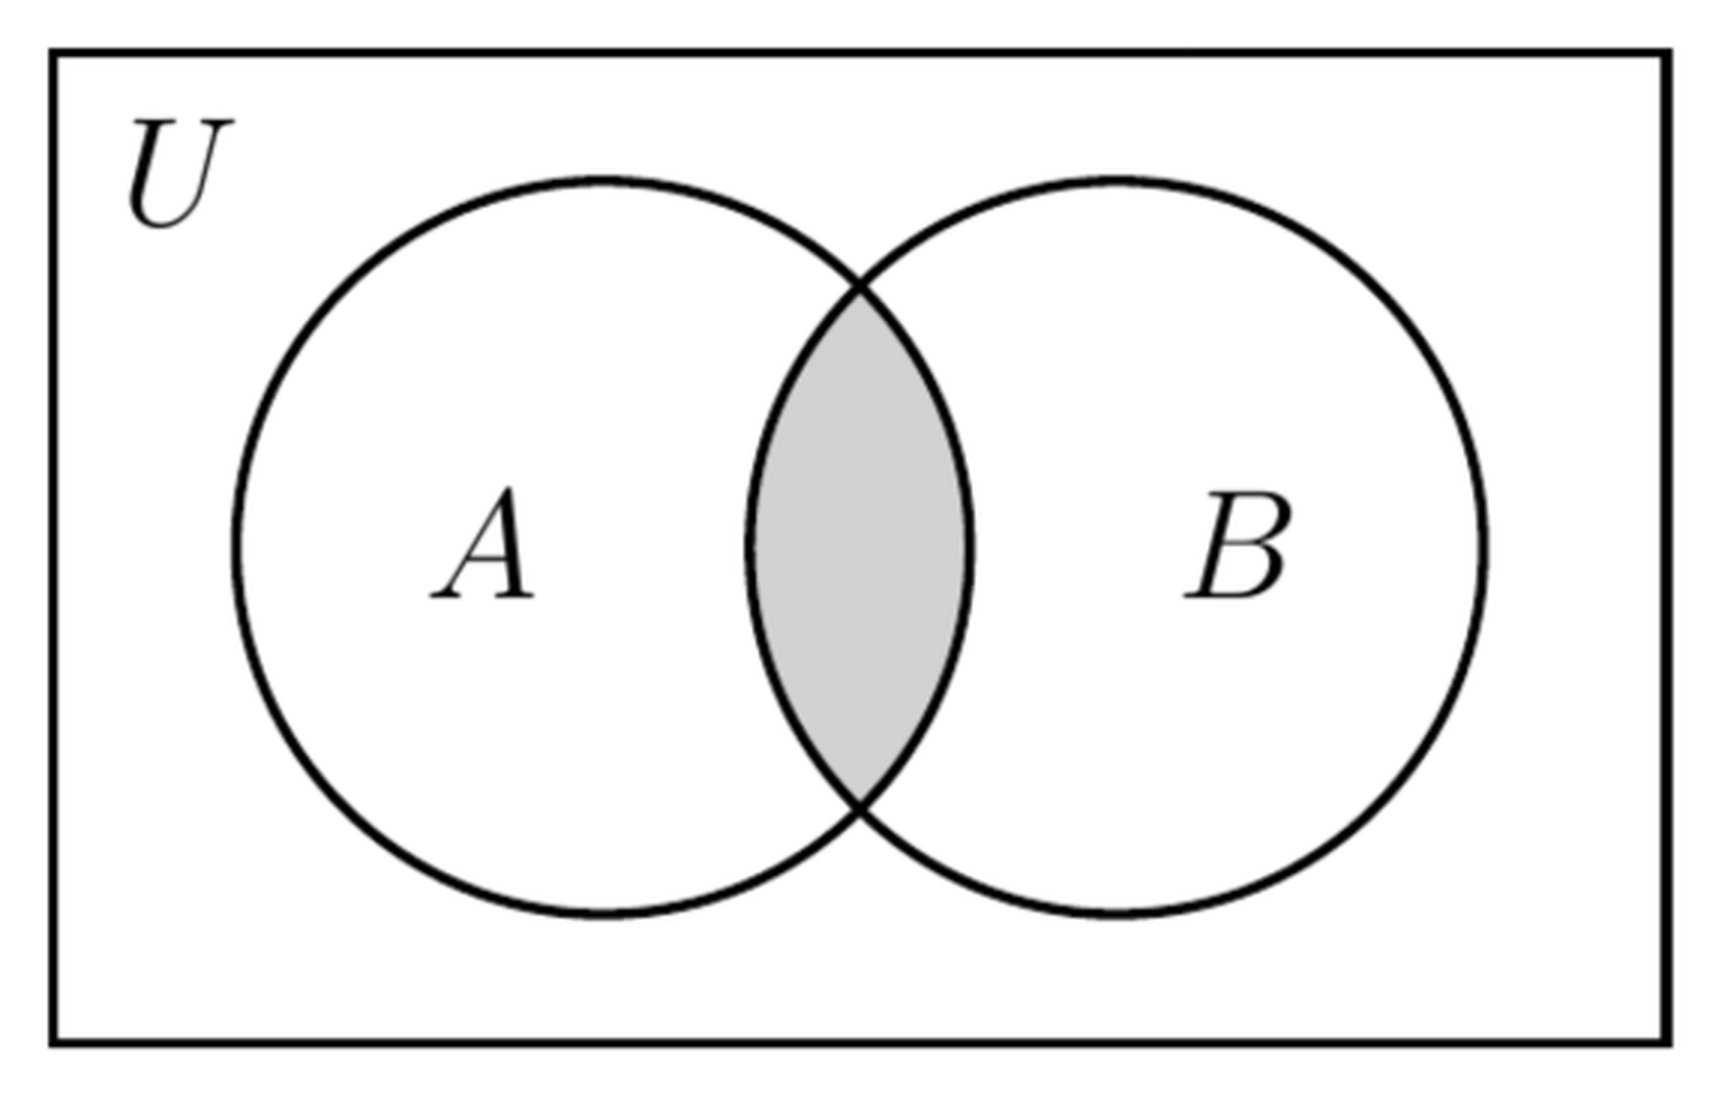
\includegraphics[width=0.38\textwidth]{figures/gao141_q5.png}
\end{center}

\ifanswer
\solbegin
\step{阴影部分表示 $A\cap B=\{4,7\}$.}
\solend
\fi

\item 方程 $2^{\log_3 x}=\dfrac12$ 的解集为\blankline[4.4em].

\ifanswer
\solbegin
\step{$2^{\log_3 x}=2^{-1}\Leftrightarrow\log_3 x=-1\Leftrightarrow x=\dfrac13$，解集为 $\left\{\dfrac13\right\}$.}
\solend
\fi

\item 若集合 $A=\left\{x\mid x^2+ax+\dfrac14=0\right\}$ 有且仅有两个子集，则实数 $a$ 的值为\blankline[4.4em].

\ifanswer
\solbegin
\step{$A$ 有且仅有两个子集，说明 $A$ 恰有一个元素，即方程有两个相等的实数根.}
\step{$\Delta=a^2-4\cdot\dfrac14=0\Rightarrow a=\pm1$.}% 判别式原卷印等腰偏高的高三角 $\Delta$，照录
\solend
\fi

\item 已知关于 $x$ 的方程 $x^2+mx+2m=0$ 的两个实数根分别为 $\alpha$、$\beta$，若 $\alpha^2+\beta^2=5$，则实数 $m=$\blankline[4.4em].

\ifanswer
\solbegin
\step{方程 $x^2+mx+2m=0$ 的两个实数根为 $\alpha$、$\beta$，}
\step{由根与系数的关系得 $\begin{cases}\alpha+\beta=-m\\\alpha\beta=2m\end{cases}$，又因为 $\alpha^2+\beta^2=5$，}
\step{所以 $\alpha^2+\beta^2=(\alpha+\beta)^2-2\alpha\beta=m^2-4m=5$，整理得 $m^2-4m-5=0$，}
\step{解得 $m=5$ 或 $m=-1$，}
\step{当 $m=5$ 时，$\triangle=25-40=-15<0$，无实根，舍去；}% 判别式原卷印扁等边三角 $\triangle$，照录
\step{当 $m=-1$ 时，$\triangle=1+8=9>0$，符合题意，}
\step{所以实数 $m=-1$.}
\solend
\fi

\item 若不等式 $\lvert x-3\rvert+\lvert x-5\rvert\geqslant a$ 对任意的实数 $x$ 恒成立，则实数 $a$ 的取值范围为\blankline[4.4em].

\ifanswer
\solbegin
\step{由三角不等式得 $\lvert x-3\rvert+\lvert x-5\rvert\geqslant\lvert x-3-x+5\rvert=2$，则 $a\leqslant2$.}
\solend
\fi

\item 设集合 $A=\{-3,2\}$，集合 $B=\{x\mid mx+1=0\}$，若 $A\cup B=A$，则实数 $m$ 的值为\blankline[4.4em].

\ifanswer
\solbegin
\step{由 $A\cup B=A$，得 $B\subseteq A$，}% 子集符号原卷印带下划线的 $\subseteq$，照录
\step{当 $m=0$ 时，$B=\varnothing$，满足题意，}
\step{当 $m\neq0$ 时，$B=\left\{-\dfrac1m\right\}$，所以 $-\dfrac1m=2$ 或 $-\dfrac1m=-3$，所以 $m=-\dfrac12$ 或 $m=\dfrac13$，}
\step{综上所述，$m=0$ 或 $m=-\dfrac12$ 或 $m=\dfrac13$.}
\solend
\fi

\item 已知 $m$ 为实数，代数式 $M=\sqrt{m-1}+\sqrt{3-m}$ 的取值范围为\blankline[4.4em].

\ifanswer
\solbegin
\step{根式有意义要求 $m\in[1,3]$，}
\step{此时 $(m-1)(3-m)=1-(m-2)^2$ 的取值范围为 $[0,1]$.}
\step{$M^2=2+2\sqrt{(m-1)(3-m)}$ 的取值范围为 $[2,4]$，又 $M>0$，}
\step{所以 $M\in[\sqrt2,2]$.}
\solend
\fi

\item 设有限集 $M$ 所含元素的个数用 $\mathbf{card}(M)$ 表示，并规定 $\mathbf{card}(\varnothing)=0$. 已知集合 $A,B$ 满足 $A\cup B=\{1,2,3\}$，$A\cap B=\varnothing$，若 $\mathbf{card}(A)\notin A$，$\mathbf{card}(B)\notin B$，则满足条件的所有不同集合 $A$ 的个数为\blankline[4.4em].

\ifanswer
\solbegin
\step{当 $\mathbf{card}(A)=0$ 或 $3$ 时，$A,B$ 中有一个为 $\{1,2,3\}$，不符合条件.}
\step{当 $\mathbf{card}(A)=1$ 时，$\mathbf{card}(B)=2\notin B$，所以 $A=\{2\}$，符合条件.}
\step{当 $\mathbf{card}(A)=2$ 时，$2\notin A$，所以 $B=\{2\}$，$A=\{1,3\}$，符合条件.}
\step{满足条件的集合 $A$ 共 $2$ 个.}
\solend
\fi

\end{enumerate}

\bigsec{二、选择题}

\begin{enumerate}
\setcounter{enumi}{12}

\item “ $x=1$ ” 是 “ $x^2-3x+2=0$ ” 的\mbox{（\quad）}条件.

\keepwithprev
A. 充分非必要\qquad B. 必要非充分

C. 充要\qquad D. 既非充分又非必要

\ifanswer
\solbegin
\step{$x^2-3x+2=0\Leftrightarrow x=1$ 或 $x=2$，所以 “ $x=1$ ” 是其充分非必要条件，}
\step{故选 $A$.}
\solend
\fi

\item 设 $a,b,c\in\R$，则下列命题为真命题的是\mbox{（\quad）}
% 原卷题干只声明 a,b,c，而 A 选项出现未声明的 d，照录（存疑）
\keepwithprev
A. 若 $a>b$ 且 $c>d$，则 $ac>bd$\qquad B. 若 $a^2>b^2$，则 $a>b$

C. 若 $ab>0$ 且 $a>b$，则 $\dfrac1a<\dfrac1b$\qquad D. 若 $a<0<b$，则 $\sqrt{-a}<\sqrt b$

\ifanswer
\solbegin
\step{$ab>0$ 且 $a>b\Rightarrow\dfrac1a-\dfrac1b=\dfrac{b-a}{ab}<0$，所以 $C$ 为真命题，故选 $C$.}
\solend
\fi

\item 已知 $\log_{14}7=a$，$14^b=5$，则 $\log_{35}28=$\mbox{（\quad）}

\keepwithprev
A. $\dfrac{2-a}{2a+b}$\qquad B. $\dfrac{2+a}{a+b}$\qquad C. $\dfrac{2-a}{a+2b}$\qquad D. $\dfrac{2-a}{a+b}$

\ifanswer
\solbegin
\step{$\log_{14}7=a$，$14^b=5$，}
\step{$\log_{35}28=\dfrac{\log_{14}28}{\log_{14}35}=\dfrac{\log_{14}14^2-\log_{14}7}{\log_{14}7+\log_{14}5}=\dfrac{2-a}{a+b}$. 故选 $D$.}
\solend
\fi

\item 关于 $x$ 的不等式 $ax^2+bx+3>0$ 的解集有下列说法，其中正确的个数是\mbox{（\quad）}

\keepwithprev
① 不等式 $ax^2+bx+3>0$ 的解集可以是 $\R$

② 不等式 $ax^2+bx+3>0$ 的解集可以是 $\{x\mid x>3\}$

③ 不等式 $ax^2+bx+3>0$ 的解集可以是 $\varnothing$

④ 不等式 $ax^2+bx+3>0$ 的解集可以是 $\{x\mid -1<x<3\}$

\keepwithprev
A. 4\qquad B. 3\qquad C. 2\qquad D. 1

\ifanswer
\solbegin
\step{$x=0$ 时左端为 $3>0$，解集必含 $0$，所以②③错误.}
\step{①取 $a=1,b=0$，$x^2+3>0$ 的解集为 $\R$，正确.}
\step{④取 $a=-1,b=2$，$-x^2+2x+3=-(x+1)(x-3)>0\Leftrightarrow-1<x<3$，正确.}
\step{正确的有①④，共 $2$ 个，故选 $C$.}
\solend
\fi

\end{enumerate}

\bigsec{三、解答题}

\begin{enumerate}
\setcounter{enumi}{16}

\item 已知集合 $A=\left\{x\mid\dfrac{x-2}{x+3}\geqslant0\right\}$，集合 $B=\{x\mid\lvert x+1\rvert+\lvert x-1\rvert<5\}$，全集 $U=\R$.

(1) 求 $A,B$；

(2) 求 $A\cup B$、$\overline{A\cap B}$.

\ifanswer
\solbegin
\step{(1) 分母不为零，且分子、分母同号或分子为零，}
\step{所以 $\dfrac{x-2}{x+3}\geqslant0\Leftrightarrow x<-3$ 或 $x\geqslant2$，因此 $A=(-\infty,-3)\cup[2,+\infty)$.}
\step{又 $\lvert x+1\rvert+\lvert x-1\rvert=\begin{cases}-2x,&x<-1\\2,&-1\leqslant x\leqslant1\\2x,&x>1\end{cases}$，}
\step{分别解得 $-\dfrac52<x<-1$、$-1\leqslant x\leqslant1$、$1<x<\dfrac52$，因此 $B=\left(-\dfrac52,\dfrac52\right)$.}
\step{(2) 合并两集合所对应的区间，得 $A\cup B=(-\infty,-3)\cup\left(-\dfrac52,+\infty\right)$，}
\step{两集合的公共部分为 $A\cap B=\left[2,\dfrac52\right)$，所以 $\overline{A\cap B}=(-\infty,2)\cup\left[\dfrac52,+\infty\right)$.}
\solend
\fi

\item (1) 已知 $a>b>0$，比较代数式 $\dfrac ab$ 与 $\dfrac{a+1}{b+1}$ 的大小并说明理由；

(2) 已知 $x,y,z$ 都是正实数，$a=x+\dfrac1y,b=y+\dfrac1z,c=z+\dfrac1x$，试用反证法证明 $a,b,c$ 至少有一个不小于 $2$.

\ifanswer
\solbegin
\step{(1) $\dfrac ab-\dfrac{a+1}{b+1}=\dfrac{a(b+1)-b(a+1)}{b(b+1)}=\dfrac{a-b}{b(b+1)}$，}
\step{因为 $a>b>0$，所以 $a-b>0$，$b(b+1)>0$，所以 $\dfrac ab-\dfrac{a+1}{b+1}>0$，}
\step{故 $\dfrac ab>\dfrac{a+1}{b+1}$.}
\step{(2) 假设 $a$、$b$、$c$ 三数都小于 $2$，则 $x+\dfrac1y+y+\dfrac1z+z+\dfrac1x<6$.}
\step{因为 $x,y,z$ 均大于 $0$，}
\step{所以 $x+\dfrac1y+y+\dfrac1z+z+\dfrac1x=x+\dfrac1x+y+\dfrac1y+z+\dfrac1z\geqslant2+2+2=6$，矛盾，}
\step{所以 $a$、$b$、$c$ 三数中至少有一个不小于 $2$.}
\solend
\fi

% 第 19 题长方体无盖贮水池砖墙示意图（题目配图，三版都出）：取原卷 06 页截图去粉色水印、LANCZOS 放大 3 倍
\needvspace{6cm}
\item 如图所示，某工厂要建造一个长方体形无盖贮水池，其容积为 $3200m^3$，深为 $2m$.

(1) 若水池的长比宽至少多 $60m$，求水池的宽的最大值；

(2) 若池底每平方米的造价为 $150$ 元，池壁每平方米的造价为 $120$ 元，那么怎样设计水池的长和宽能使总造价最低？最低总造价是多少？

\begin{center}
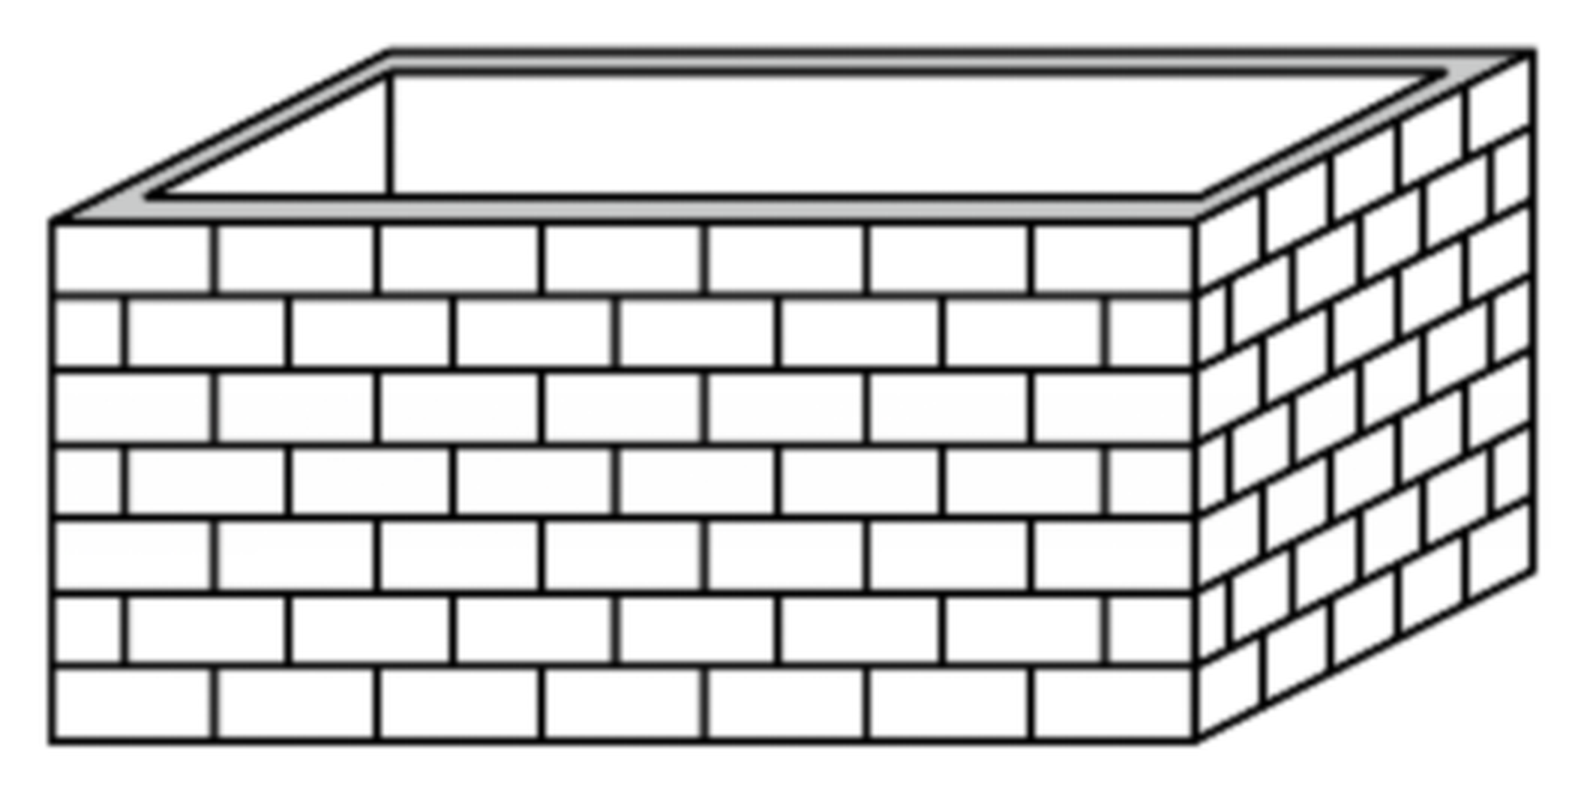
\includegraphics[width=0.42\textwidth]{figures/gao141_q19.png}
\end{center}

\ifanswer
\solbegin
\step{(1) 设水池的长、宽分别为 $xm$，$ym$，则 $x-y\geqslant60$，且 $x$、$y>0$，}
\step{由题意得 $2xy=3200$，即 $x=\dfrac{1600}{y}$，所以 $\dfrac{1600}{y}-y\geqslant60$，}
\step{因为 $y>0$，所以 $1600-y^2\geqslant60y$，}
\step{即 $y^2+60y-1600=(y+80)(y-20)\leqslant0$，解得 $-80\leqslant y\leqslant20$，}
\step{又 $y>0$，所以 $0<y\leqslant20$，所以水池的宽的最大值为 $20m$.}
\step{(2) 设水池总造价为 $z$ 元，}
\step{则 $z=1600\times150+2\times(2x+2y)\times120=240000+480(x+y)$，}
\step{又因为 $y=\dfrac{1600}{x}$，}
\step{所以 $z=240000+\left(x+\dfrac{1600}{x}\right)\times480\geqslant240000+480\times2\sqrt{1600}$}
\step{$=240000+38400=278400$，}
\step{当且仅当 $x=\dfrac{1600}{x}$，即 $x=y=40$ 时取等号，}
\step{所以，将水池的池底设计为边长为 $40m$ 的正方形时总造价最低，}
\step{最低总造价为 $278400$ 元.}
\solend
\fi

\item 已知 $a\in\R$，设集合 $A=\{x\mid ax^2-3x+2<ax-1\}$.

(1) 若 $A=(1,3)$，求实数 $a$ 的值；

(2) 当 $a>0$ 时，求 $A$；

(3) 若 “ $x\in\left(\dfrac12,+\infty\right)$ ” 是 “ $x\in A$ ” 的必要非充分条件，求实数 $a$ 的取值范围.

\ifanswer
\solbegin
\step{原不等式等价于 $ax^2-(a+3)x+3<0\Leftrightarrow(x-1)(ax-3)<0$，}
\step{(1) $A=(1,3)$ 为有界区间，因此 $a>0$，两根为 $1$ 和 $\dfrac3a$，于是 $\dfrac3a=3$，得 $a=1$；}
\step{此时 $(x-1)(x-3)<0$ 的解集确为 $(1,3)$.}
\step{(2) 当 $a>0$ 时，二次项系数为正，比较 $1$ 与 $\dfrac3a$，得 $A=\begin{cases}\left(1,\dfrac3a\right),&0<a<3\\\varnothing,&a=3\\\left(\dfrac3a,1\right),&a>3\end{cases}$，}
\step{其中 $a=3$ 时，原不等式为 $3(x-1)^2<0$，无解.}
\step{(3) 记 $S=\left(\dfrac12,+\infty\right)$，题意要求 $A\subset S$.}% 子集符号原卷印单线 $\subset$，照录
\step{由于对任意 $a$ 都有 $1\notin A$，而 $1\in S$，所以只需满足 $A\subseteq S$.}
\step{当 $a<0$ 时，$A=\left(-\infty,\dfrac3a\right)\cup(1,+\infty)$，含有小于 $\dfrac12$ 的数，不符合条件.}
\step{当 $a=0$ 时，$A=(1,+\infty)$，符合条件.}
\step{当 $0<a<3$ 时，$A=\left(1,\dfrac3a\right)\subseteq S$；}
\step{当 $a=3$ 时，$A=\varnothing\subseteq S$，均符合条件；}
\step{当 $a>3$ 时，$A=\left(\dfrac3a,1\right)$，所以 $A\subseteq S\Leftrightarrow\dfrac3a\geqslant\dfrac12\Leftrightarrow a\leqslant6$；}
\step{因此实数 $a$ 的取值范围为 $[0,6]$.}
\solend
\fi

\item 甲、乙两同学探讨了一个问题：已知正实数 $x,y$ 满足 $3x+y=1$，求 $\dfrac1x+\dfrac1y$ 的最小值.

甲给出的解法：由 $1=3x+y\geqslant2\sqrt{3xy}$，得 $\sqrt{xy}\leqslant\dfrac{\sqrt3}{6}$，所以 $\dfrac1x+\dfrac1y\geqslant2\sqrt{\dfrac1{xy}}\geqslant4\sqrt3$. 因此 $\dfrac1x+\dfrac1y$ 的最小值为 $4\sqrt3$.

乙给出的解法：$\dfrac1x+\dfrac1y=\left(\dfrac1x+\dfrac1y\right)(3x+y)=4+\dfrac yx+\dfrac{3x}{y}$，因为 $x,y$ 均为正实数，所以 $\dfrac1x+\dfrac1y\geqslant4+2\sqrt{\dfrac yx\cdot\dfrac{3x}{y}}=4+2\sqrt3$.

(1) 请判断上述哪位同学的解法正确，哪位同学的解法错误，并指出错误的原因；

(2) 结合上述探讨，试求当 $0<x<\dfrac12$ 时，$\dfrac1x+\dfrac1{1-2x}$ 的最小值以及此时实数 $x$ 的值；

(3) 已知 $x$ 为正实数，$y$ 为非负实数，且 $x+2y=2$，求 $\dfrac{x^2+1}{x}+\dfrac{2y^2}{y+1}$ 的最小值以及此时实数 $x,y$ 的值.

\ifanswer
\solbegin
\step{(1) 甲的推导中，$3x+y\geqslant2\sqrt{3xy}$ 取等号要求 $3x=y$，}
\step{$\dfrac1x+\dfrac1y\geqslant\dfrac2{\sqrt{xy}}$ 取等号要求 $x=y$，两者对正实数 $x,y$ 不能同时成立，}
\step{因此不能将 $4\sqrt3$ 判为最小值，甲错误.}
\step{乙的等号条件为 $\dfrac yx=\dfrac{3x}{y}$，即 $y=\sqrt3 x$；}
\step{结合 $3x+y=1$，得 $x=\dfrac1{3+\sqrt3},y=\dfrac{\sqrt3}{3+\sqrt3}$ 均为正数，等号可以成立，}
\step{因此乙正确，最小值为 $4+2\sqrt3$.}
\step{(2) 令 $t=1-2x>0$，则 $2x+t=1$.}
\step{$\dfrac1x+\dfrac1t=\left(\dfrac1x+\dfrac1t\right)(2x+t)=3+\dfrac tx+\dfrac{2x}{t}\geqslant3+2\sqrt2$，}
\step{当且仅当 $\dfrac tx=\dfrac{2x}{t}$，即 $t=\sqrt2 x$ 时取等号，}
\step{由 $2x+t=1$，得 $x=\dfrac1{2+\sqrt2}=\dfrac{2-\sqrt2}{2}\in\left(0,\dfrac12\right)$，}
\step{因此最小值为 $3+2\sqrt2$，此时 $x=\dfrac{2-\sqrt2}{2}$.}
\step{(3) 记目标式为 $F$，利用 $x+2y=2$，}
\step{得 $F=x+\dfrac1x+2y-2+\dfrac2{y+1}=\dfrac1x+\dfrac2{y+1}$，}
\step{又 $x+2(y+1)=4$，且 $x>0$、$y+1>0$，}
\step{所以 $4F=\left(\dfrac1x+\dfrac2{y+1}\right)(x+2(y+1))=5+2\left(\dfrac{y+1}{x}+\dfrac{x}{y+1}\right)$}
\step{$\geqslant5+2\times2=9$，当且仅当 $\dfrac{y+1}{x}=\dfrac{x}{y+1}$，即 $x=y+1$ 时取等号.}
\step{联立 $x+2y=2$，得 $x=\dfrac43$、$y=\dfrac13$，满足题设条件，}
\step{因此最小值为 $\dfrac94$，此时 $x=\dfrac43$，$y=\dfrac13$.}
\solend
\fi

\end{enumerate}

\end{document}
"
% 紧凑版：xelatex "\def\iscompact{1}% 高一141_彭浦中学_期中.tex
%   —— 高一上数学"2026-2027 年彭浦中学高一上期中"（试卷版/答案版/紧凑版）
% 试卷版：xelatex 高一141_彭浦中学_期中.tex
% 答案版：xelatex "\def\isanswer{1}% 高一141_彭浦中学_期中.tex
%   —— 高一上数学"2026-2027 年彭浦中学高一上期中"（试卷版/答案版/紧凑版）
% 试卷版：xelatex 高一141_彭浦中学_期中.tex
% 答案版：xelatex "\def\isanswer{1}% 高一141_彭浦中学_期中.tex
%   —— 高一上数学"2026-2027 年彭浦中学高一上期中"（试卷版/答案版/紧凑版）
% 试卷版：xelatex 高一141_彭浦中学_期中.tex
% 答案版：xelatex "\def\isanswer{1}\input{高一141_彭浦中学_期中.tex}"
% 紧凑版：xelatex "\def\iscompact{1}\input{高一141_彭浦中学_期中.tex}"
%
% ① 原始材料：微信公众号"魔都数学加油站"文章，连载"27学年高一141"，原文标题
% "27学年高一141——2026-2027年上海市彭浦中学高一上期中"；
% 原文链接：https://mp.weixin.qq.com/s/V_8bEhC6geeFyQysmtqUtQ。
% 正文为 9 张 PNG 页（01、05、06、07、09 为 2560x3620；02、03、04、08 为 4762x6735，
% 同一篇各页分辨率不同，逐页按各自分辨率放大裁图核对），题目下印【解析】，为讲评版。
% 题目、解析均据原图转录；卷面粉红色水印"魔都数学加油站"及公众号页脚未录入。
% 全卷 2 幅插图，均属题目配图（在 \ifanswer 外、三版都出）、取原卷截图去粉色水印、
% LANCZOS 放大 3 倍：第 5 题韦恩图（01 页，全集 U 矩形内两圆相交、交集阴影、A/B/U 标注）、
% 第 19 题长方体无盖贮水池砖墙示意图（06 页右上）。通读 9 页确认除这 2 幅外无其它
% 插图/表格，亦无"题干写如图而源码漏图"（仅 Q5"图中阴影部分"、Q19"如图所示"两处提到图）。
%
% 卷首标题：原卷印作"2026-2027 年彭浦中学高一上期中"（公众号标题中的"上海市"
% 卷面标题行没有，本稿照卷面），年份区间按全稿惯例排 en dash；原卷未印副标题，
% 本卷为期中卷、跨集合与常用逻辑用语／不等式／函数三章，按题目内容补出
% "集合与常用逻辑用语、不等式、函数"（与 高一140 同期中卷口径相同）：
% 集合与逻辑见 Q5、Q10、Q12、Q13、Q16、Q17、Q20，不等式见 Q4、Q9、Q14、Q18、
% Q19、Q21，函数（指数／对数）见 Q6、Q15。
%
% 题号体例：本卷共 19 题——一、填空题 3—12（10 题）、二、选择题 13—16（4 题）、
% 三、解答题 17—21（5 题）。三节分别 \setcounter{enumi}{2}／{12}／{16}。
% 原卷从第 3 题起、无第 1、2 题，本稿保留原题号；全卷无附加题节。
%
% ② 与原卷的排版差异：
%   ① 原文从第 3 题起，本稿保留原题号；
%   ② 原卷 19 题题下均印【解析】，无独立【答案】段、无"答案印题干括号且无解析"、
%      无"只印【答案】无解析"一型：填空题与解答题的答案落在【解析】末句
%      （Q3—Q12、Q17—Q21），四道选择题答案在【解析】末句"故选 …"
%      （Q13 选 A、Q14 选 C、Q15 选 D、Q16 选 C），题干括号内一律留空；
%      本稿 19 题一律 \solbegin…\solend、全卷不提 \ans{}，答案版【解析】标记数
%      = 19 = 全卷题数（无【答案】标记）；
%   ③ 原卷未印副标题，本稿按"知识模块"口径补出；
%   ④ 原卷填空横线按全稿惯例排 \blankline[4.4em]；选择题括号排 \mbox{（\quad）}，
%      选项段／命题段前按惯例加 \keepwithprev（Q16 两枚：命题列与选项段各一）；
%      解答题不留作答区、不加 \anspace（原卷为讲评版，与 129／131／132／133／136／140 同）；
%   ⑤ 原卷数集混排：黑板粗体 R（Q14 题干、Q16 ① 与解析、Q17 全集、Q20 题干）
%      按全稿惯例统一改 \R；空集记号 \varnothing；绝对值排 \lvert…\rvert，
%      集合描述竖线排 \mid；不等号按全稿惯例排 \leqslant／\geqslant；
%      补集照原卷上划线排 \overline{A\cap B}（Q17(2) 题干与解析）；
%      原卷"card"记号排黑体正体（Q12），本稿照录 \mathbf{card}，未改斜体
%      （与 高一66 同题口径不同：那份原卷 card 排斜体、照录 $card(M)$）；
%   ⑥ 子题标号 (1)(2)(3) 原卷印半角括号，照录；圈数字 ①②③④ 在正文（文本模式）
%      按原卷照录，未进数学式；数学式内半角逗号照录（如 Q12"$A,B$"、"{1,2,3}"、
%      Q14"$a,b,c\in\R$"、Q15"$\log_{14}7=a$，$14^b=5$"、Q16"$a=1,b=0$"、
%      Q18"$x,y,z$"、Q20"$x,y$"、Q21"$x,y$"）；全卷行末西文句点照录为 ASCII 句点；
%      行中全角逗号、顿号照录；
%   ⑦ 题干中的中文弯引号按原卷照录（Q13、Q20(3) 的 “ ” 及引号内空格），
%      注释内一律 ASCII 引号；
%   ⑧ 两幅题目配图各在 \item 之前加 \needvspace 守卫整块推走（Q5 5cm、Q19 6cm），
%      守卫放在 \item 之前而非 \bigsec 之后——两题均非各节首题，不触发 B 类
%      "节标题落页末"（照 高一26／40／59／136／140 成例）；三版切页审计均"合计异常：无"；
%   ⑨ 跨页续印按题合并：Q8 题干与【解析】首行在 01 页、后 6 行在 02 页；
%      Q15 题干在 03 页、【解析】在 04 页；Q17 题干与【解析】前 2 行在 04 页、
%      后 4 行在 05 页；Q19 题干在 05 页末、(1)(2) 小问与砖墙图与【解析】在 06 页；
%      Q20 题干 (1)(2) 在 06 页末、(3) 与【解析】在 07 页；Q21 题干与【解析】
%      前 6 行在 08 页、后 12 行在 09 页；Q16、Q18 全在各自页内；
%      本稿按题连排，不丢行；
%   ⑩ 原卷无红色加粗标签（【解析】均黑色印刷，Q16 解析 "①取…""④取…" 与
%      Q20 解析 "(2)" 等分步标签亦黑色），故本卷未用 \stepm；
%   ⑪ 原卷 Q19 题干把数值与单位（3200m³、2m、60m、150 元、120 元、40m、20m、
%      278400 元）印作略粗的西文字形，本稿按全稿惯例（高一70／72 同类题）排普通
%      数学体，未加粗。
%
% ③ 行数复核：一条 \step = 原卷解析的一个印刷行，cases 块作一个印刷行计。逐题数 \step
%   条数，合计 92 条（Q3：1；Q4：1；Q5：1；Q6：1；Q7：2；Q8：7；Q9：1；Q10：4；
%   Q11：4；Q12：4；Q13：2；Q14：1；Q15：2；Q16：4；Q17：6；Q18：7；Q19：13；
%   Q20：13；Q21：18），与原卷印刷行逐题相等。全卷 19 题均印【解析】、无独立 \ans{}，
%   答案版【解析】标记数 = 19 = 全卷题数。
%
% ④ 判别式／子集符号结论（逐处放大原图照录、不得统一）：
%   判别式：全卷 3 处——第 7 题【解析】"$\Delta=a^2-4\cdot\frac14=0$"一处原卷印
%     等腰、偏高的高三角 $\Delta$，照录 \Delta；第 8 题【解析】
%     "$\triangle=25-40=-15<0$"与"$\triangle=1+8=9>0$"两处原卷印扁等边三角
%     $\triangle$，照录 \triangle。两形不同，逐处照录未统一。
%   子集：全卷 6 处——第 10 题【解析】"$B\subseteq A$"一处、第 20 题【解析】
%     "所以只需满足 $A\subseteq S$"、"$A=\left(1,\frac3a\right)\subseteq S$"、
%     "$A=\varnothing\subseteq S$"、"$A\subseteq S\Leftrightarrow\frac3a\geqslant\frac12$"
%     四处，共 5 处原卷印带下划线的 $\subseteq$，照录 \subseteq；第 20 题【解析】
%     (3) 首行"题意要求 $A\subset S$"一处原卷印单线 $\subset$，照录 \subset
%     （下行因 $1\in S$ 而 $1\notin A$，改述为 $A\subseteq S$，两者逻辑一致、非笔误）。
%
% ⑤ 存疑照录（照录未改，正文对应处另有 % 注）：
%   第 14 题题干"设 $a,b,c\in\R$"只声明 $a,b,c$，而 A 选项"若 $a>b$ 且 $c>d$，
%     则 $ac>bd$"引入未声明的 $d$，原卷变量声明与选项不统一，照录未补。
%   全卷除此 1 条外未发现其它笔误／自相矛盾处。
%
% ⑥ 跨页续印按题合并说明：见 ② ⑨。
%
\documentclass[a4paper,11pt]{article}
\usepackage{common}

\begin{document}

\examtitlest[3]{2026--2027 年彭浦中学高一上期中}{集合与常用逻辑用语、不等式、函数}

\bigsec{一、填空题}

\begin{enumerate}
\setcounter{enumi}{2}

\item 已知 $m$ 为实数，若 $1\in\{m,m^2\}$，则 $m$ 的值为\blankline[4.4em].

\ifanswer
\solbegin
\step{$m=1$ 或 $m^2=1$，得 $m=\pm1$；按列举项互异口径排除 $m=m^2=1$，得 $m=-1$.}
\solend
\fi

\item 已知 $2<a<4$，$-2<b<1$，则 $2a+b$ 的取值范围为\blankline[4.4em].

\ifanswer
\solbegin
\step{$4<2a<8$，与 $-2<b<1$ 相加，得 $2<2a+b<9$，取值范围为 $(2,9)$.}
\solend
\fi

% 第 5 题韦恩图（题目配图，三版都出）：取原卷 01 页截图去粉色水印、LANCZOS 放大 3 倍
\needvspace{5cm}
\item 已知集合 $A=\{-1,-2,1,4,7\}$，$B=\{x\mid x>1\}$，用列举法表示图中阴影部分所表示的集合为\blankline[4.4em].

\begin{center}
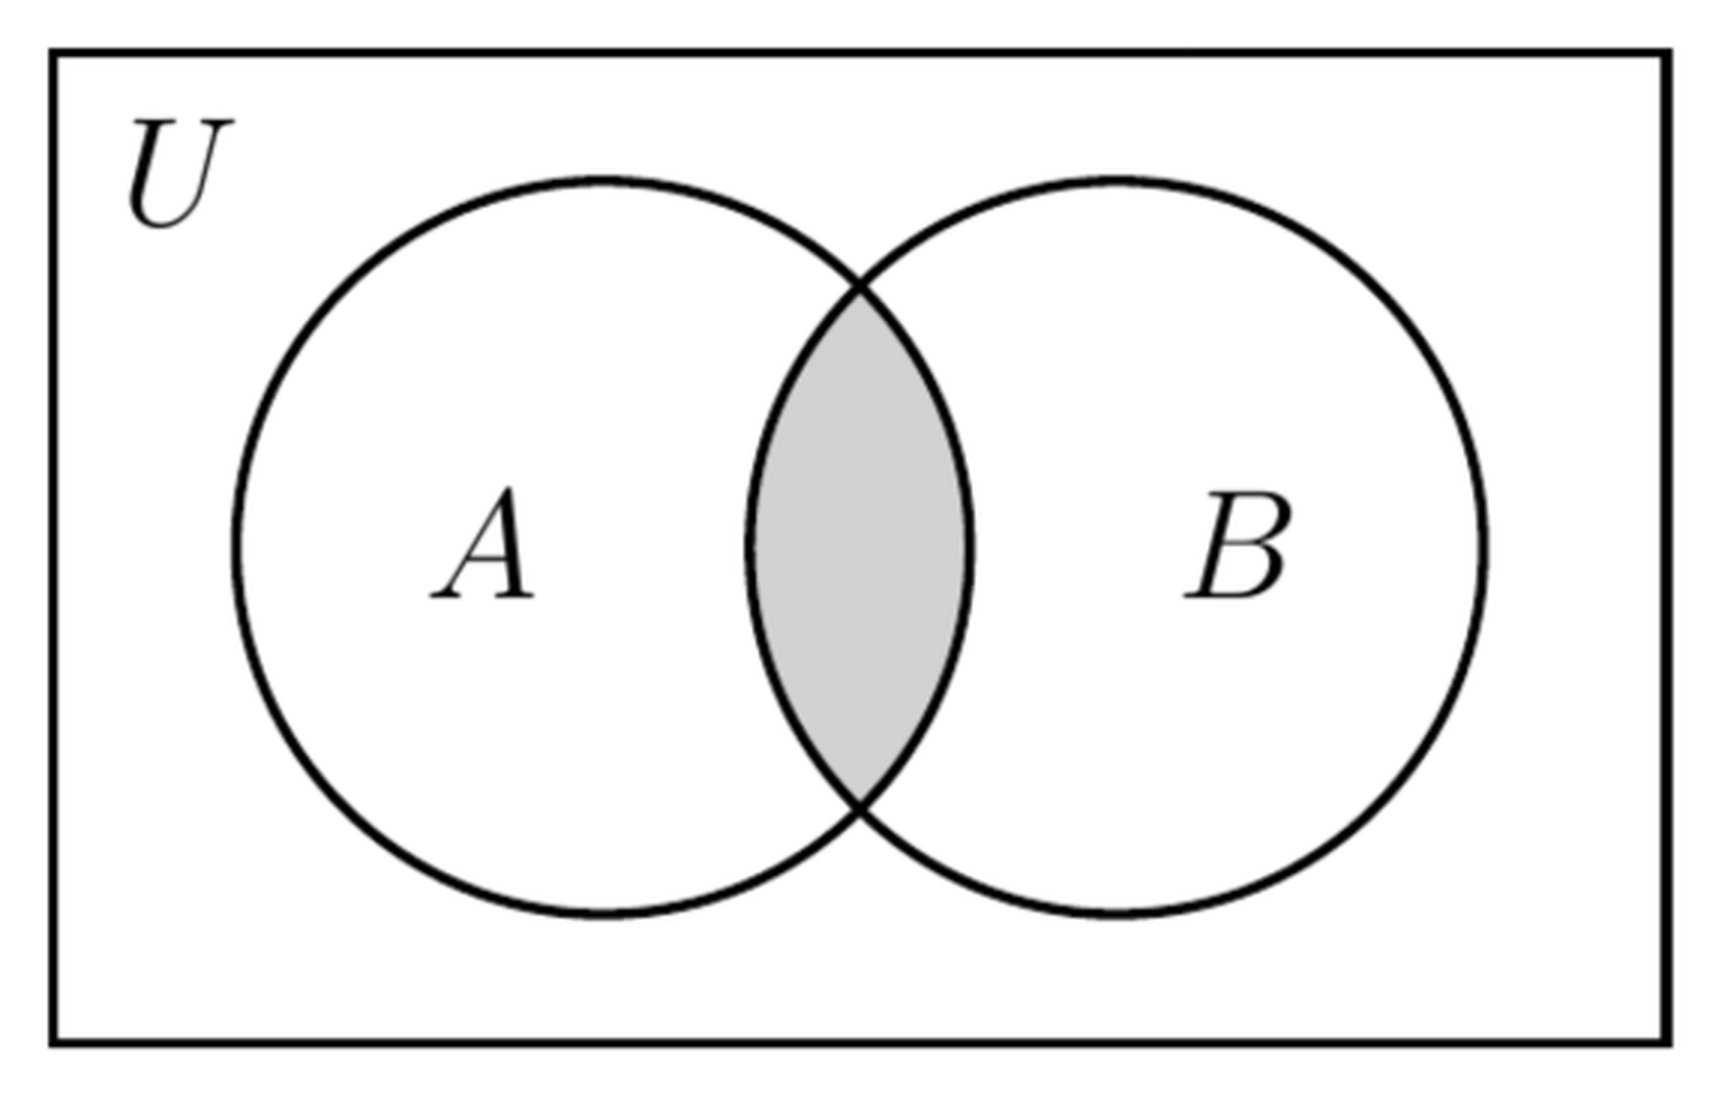
\includegraphics[width=0.38\textwidth]{figures/gao141_q5.png}
\end{center}

\ifanswer
\solbegin
\step{阴影部分表示 $A\cap B=\{4,7\}$.}
\solend
\fi

\item 方程 $2^{\log_3 x}=\dfrac12$ 的解集为\blankline[4.4em].

\ifanswer
\solbegin
\step{$2^{\log_3 x}=2^{-1}\Leftrightarrow\log_3 x=-1\Leftrightarrow x=\dfrac13$，解集为 $\left\{\dfrac13\right\}$.}
\solend
\fi

\item 若集合 $A=\left\{x\mid x^2+ax+\dfrac14=0\right\}$ 有且仅有两个子集，则实数 $a$ 的值为\blankline[4.4em].

\ifanswer
\solbegin
\step{$A$ 有且仅有两个子集，说明 $A$ 恰有一个元素，即方程有两个相等的实数根.}
\step{$\Delta=a^2-4\cdot\dfrac14=0\Rightarrow a=\pm1$.}% 判别式原卷印等腰偏高的高三角 $\Delta$，照录
\solend
\fi

\item 已知关于 $x$ 的方程 $x^2+mx+2m=0$ 的两个实数根分别为 $\alpha$、$\beta$，若 $\alpha^2+\beta^2=5$，则实数 $m=$\blankline[4.4em].

\ifanswer
\solbegin
\step{方程 $x^2+mx+2m=0$ 的两个实数根为 $\alpha$、$\beta$，}
\step{由根与系数的关系得 $\begin{cases}\alpha+\beta=-m\\\alpha\beta=2m\end{cases}$，又因为 $\alpha^2+\beta^2=5$，}
\step{所以 $\alpha^2+\beta^2=(\alpha+\beta)^2-2\alpha\beta=m^2-4m=5$，整理得 $m^2-4m-5=0$，}
\step{解得 $m=5$ 或 $m=-1$，}
\step{当 $m=5$ 时，$\triangle=25-40=-15<0$，无实根，舍去；}% 判别式原卷印扁等边三角 $\triangle$，照录
\step{当 $m=-1$ 时，$\triangle=1+8=9>0$，符合题意，}
\step{所以实数 $m=-1$.}
\solend
\fi

\item 若不等式 $\lvert x-3\rvert+\lvert x-5\rvert\geqslant a$ 对任意的实数 $x$ 恒成立，则实数 $a$ 的取值范围为\blankline[4.4em].

\ifanswer
\solbegin
\step{由三角不等式得 $\lvert x-3\rvert+\lvert x-5\rvert\geqslant\lvert x-3-x+5\rvert=2$，则 $a\leqslant2$.}
\solend
\fi

\item 设集合 $A=\{-3,2\}$，集合 $B=\{x\mid mx+1=0\}$，若 $A\cup B=A$，则实数 $m$ 的值为\blankline[4.4em].

\ifanswer
\solbegin
\step{由 $A\cup B=A$，得 $B\subseteq A$，}% 子集符号原卷印带下划线的 $\subseteq$，照录
\step{当 $m=0$ 时，$B=\varnothing$，满足题意，}
\step{当 $m\neq0$ 时，$B=\left\{-\dfrac1m\right\}$，所以 $-\dfrac1m=2$ 或 $-\dfrac1m=-3$，所以 $m=-\dfrac12$ 或 $m=\dfrac13$，}
\step{综上所述，$m=0$ 或 $m=-\dfrac12$ 或 $m=\dfrac13$.}
\solend
\fi

\item 已知 $m$ 为实数，代数式 $M=\sqrt{m-1}+\sqrt{3-m}$ 的取值范围为\blankline[4.4em].

\ifanswer
\solbegin
\step{根式有意义要求 $m\in[1,3]$，}
\step{此时 $(m-1)(3-m)=1-(m-2)^2$ 的取值范围为 $[0,1]$.}
\step{$M^2=2+2\sqrt{(m-1)(3-m)}$ 的取值范围为 $[2,4]$，又 $M>0$，}
\step{所以 $M\in[\sqrt2,2]$.}
\solend
\fi

\item 设有限集 $M$ 所含元素的个数用 $\mathbf{card}(M)$ 表示，并规定 $\mathbf{card}(\varnothing)=0$. 已知集合 $A,B$ 满足 $A\cup B=\{1,2,3\}$，$A\cap B=\varnothing$，若 $\mathbf{card}(A)\notin A$，$\mathbf{card}(B)\notin B$，则满足条件的所有不同集合 $A$ 的个数为\blankline[4.4em].

\ifanswer
\solbegin
\step{当 $\mathbf{card}(A)=0$ 或 $3$ 时，$A,B$ 中有一个为 $\{1,2,3\}$，不符合条件.}
\step{当 $\mathbf{card}(A)=1$ 时，$\mathbf{card}(B)=2\notin B$，所以 $A=\{2\}$，符合条件.}
\step{当 $\mathbf{card}(A)=2$ 时，$2\notin A$，所以 $B=\{2\}$，$A=\{1,3\}$，符合条件.}
\step{满足条件的集合 $A$ 共 $2$ 个.}
\solend
\fi

\end{enumerate}

\bigsec{二、选择题}

\begin{enumerate}
\setcounter{enumi}{12}

\item “ $x=1$ ” 是 “ $x^2-3x+2=0$ ” 的\mbox{（\quad）}条件.

\keepwithprev
A. 充分非必要\qquad B. 必要非充分

C. 充要\qquad D. 既非充分又非必要

\ifanswer
\solbegin
\step{$x^2-3x+2=0\Leftrightarrow x=1$ 或 $x=2$，所以 “ $x=1$ ” 是其充分非必要条件，}
\step{故选 $A$.}
\solend
\fi

\item 设 $a,b,c\in\R$，则下列命题为真命题的是\mbox{（\quad）}
% 原卷题干只声明 a,b,c，而 A 选项出现未声明的 d，照录（存疑）
\keepwithprev
A. 若 $a>b$ 且 $c>d$，则 $ac>bd$\qquad B. 若 $a^2>b^2$，则 $a>b$

C. 若 $ab>0$ 且 $a>b$，则 $\dfrac1a<\dfrac1b$\qquad D. 若 $a<0<b$，则 $\sqrt{-a}<\sqrt b$

\ifanswer
\solbegin
\step{$ab>0$ 且 $a>b\Rightarrow\dfrac1a-\dfrac1b=\dfrac{b-a}{ab}<0$，所以 $C$ 为真命题，故选 $C$.}
\solend
\fi

\item 已知 $\log_{14}7=a$，$14^b=5$，则 $\log_{35}28=$\mbox{（\quad）}

\keepwithprev
A. $\dfrac{2-a}{2a+b}$\qquad B. $\dfrac{2+a}{a+b}$\qquad C. $\dfrac{2-a}{a+2b}$\qquad D. $\dfrac{2-a}{a+b}$

\ifanswer
\solbegin
\step{$\log_{14}7=a$，$14^b=5$，}
\step{$\log_{35}28=\dfrac{\log_{14}28}{\log_{14}35}=\dfrac{\log_{14}14^2-\log_{14}7}{\log_{14}7+\log_{14}5}=\dfrac{2-a}{a+b}$. 故选 $D$.}
\solend
\fi

\item 关于 $x$ 的不等式 $ax^2+bx+3>0$ 的解集有下列说法，其中正确的个数是\mbox{（\quad）}

\keepwithprev
① 不等式 $ax^2+bx+3>0$ 的解集可以是 $\R$

② 不等式 $ax^2+bx+3>0$ 的解集可以是 $\{x\mid x>3\}$

③ 不等式 $ax^2+bx+3>0$ 的解集可以是 $\varnothing$

④ 不等式 $ax^2+bx+3>0$ 的解集可以是 $\{x\mid -1<x<3\}$

\keepwithprev
A. 4\qquad B. 3\qquad C. 2\qquad D. 1

\ifanswer
\solbegin
\step{$x=0$ 时左端为 $3>0$，解集必含 $0$，所以②③错误.}
\step{①取 $a=1,b=0$，$x^2+3>0$ 的解集为 $\R$，正确.}
\step{④取 $a=-1,b=2$，$-x^2+2x+3=-(x+1)(x-3)>0\Leftrightarrow-1<x<3$，正确.}
\step{正确的有①④，共 $2$ 个，故选 $C$.}
\solend
\fi

\end{enumerate}

\bigsec{三、解答题}

\begin{enumerate}
\setcounter{enumi}{16}

\item 已知集合 $A=\left\{x\mid\dfrac{x-2}{x+3}\geqslant0\right\}$，集合 $B=\{x\mid\lvert x+1\rvert+\lvert x-1\rvert<5\}$，全集 $U=\R$.

(1) 求 $A,B$；

(2) 求 $A\cup B$、$\overline{A\cap B}$.

\ifanswer
\solbegin
\step{(1) 分母不为零，且分子、分母同号或分子为零，}
\step{所以 $\dfrac{x-2}{x+3}\geqslant0\Leftrightarrow x<-3$ 或 $x\geqslant2$，因此 $A=(-\infty,-3)\cup[2,+\infty)$.}
\step{又 $\lvert x+1\rvert+\lvert x-1\rvert=\begin{cases}-2x,&x<-1\\2,&-1\leqslant x\leqslant1\\2x,&x>1\end{cases}$，}
\step{分别解得 $-\dfrac52<x<-1$、$-1\leqslant x\leqslant1$、$1<x<\dfrac52$，因此 $B=\left(-\dfrac52,\dfrac52\right)$.}
\step{(2) 合并两集合所对应的区间，得 $A\cup B=(-\infty,-3)\cup\left(-\dfrac52,+\infty\right)$，}
\step{两集合的公共部分为 $A\cap B=\left[2,\dfrac52\right)$，所以 $\overline{A\cap B}=(-\infty,2)\cup\left[\dfrac52,+\infty\right)$.}
\solend
\fi

\item (1) 已知 $a>b>0$，比较代数式 $\dfrac ab$ 与 $\dfrac{a+1}{b+1}$ 的大小并说明理由；

(2) 已知 $x,y,z$ 都是正实数，$a=x+\dfrac1y,b=y+\dfrac1z,c=z+\dfrac1x$，试用反证法证明 $a,b,c$ 至少有一个不小于 $2$.

\ifanswer
\solbegin
\step{(1) $\dfrac ab-\dfrac{a+1}{b+1}=\dfrac{a(b+1)-b(a+1)}{b(b+1)}=\dfrac{a-b}{b(b+1)}$，}
\step{因为 $a>b>0$，所以 $a-b>0$，$b(b+1)>0$，所以 $\dfrac ab-\dfrac{a+1}{b+1}>0$，}
\step{故 $\dfrac ab>\dfrac{a+1}{b+1}$.}
\step{(2) 假设 $a$、$b$、$c$ 三数都小于 $2$，则 $x+\dfrac1y+y+\dfrac1z+z+\dfrac1x<6$.}
\step{因为 $x,y,z$ 均大于 $0$，}
\step{所以 $x+\dfrac1y+y+\dfrac1z+z+\dfrac1x=x+\dfrac1x+y+\dfrac1y+z+\dfrac1z\geqslant2+2+2=6$，矛盾，}
\step{所以 $a$、$b$、$c$ 三数中至少有一个不小于 $2$.}
\solend
\fi

% 第 19 题长方体无盖贮水池砖墙示意图（题目配图，三版都出）：取原卷 06 页截图去粉色水印、LANCZOS 放大 3 倍
\needvspace{6cm}
\item 如图所示，某工厂要建造一个长方体形无盖贮水池，其容积为 $3200m^3$，深为 $2m$.

(1) 若水池的长比宽至少多 $60m$，求水池的宽的最大值；

(2) 若池底每平方米的造价为 $150$ 元，池壁每平方米的造价为 $120$ 元，那么怎样设计水池的长和宽能使总造价最低？最低总造价是多少？

\begin{center}
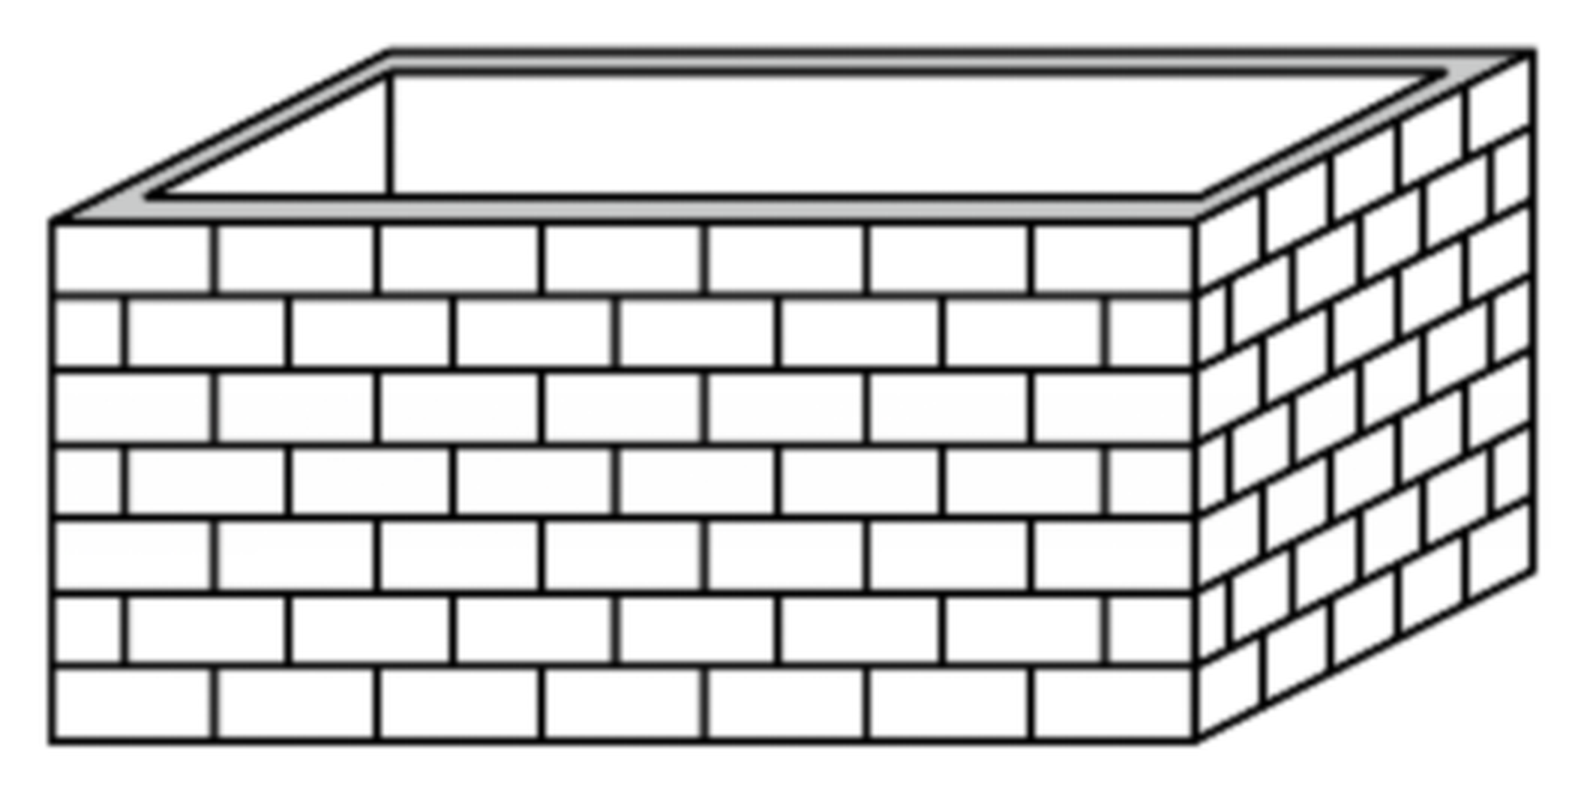
\includegraphics[width=0.42\textwidth]{figures/gao141_q19.png}
\end{center}

\ifanswer
\solbegin
\step{(1) 设水池的长、宽分别为 $xm$，$ym$，则 $x-y\geqslant60$，且 $x$、$y>0$，}
\step{由题意得 $2xy=3200$，即 $x=\dfrac{1600}{y}$，所以 $\dfrac{1600}{y}-y\geqslant60$，}
\step{因为 $y>0$，所以 $1600-y^2\geqslant60y$，}
\step{即 $y^2+60y-1600=(y+80)(y-20)\leqslant0$，解得 $-80\leqslant y\leqslant20$，}
\step{又 $y>0$，所以 $0<y\leqslant20$，所以水池的宽的最大值为 $20m$.}
\step{(2) 设水池总造价为 $z$ 元，}
\step{则 $z=1600\times150+2\times(2x+2y)\times120=240000+480(x+y)$，}
\step{又因为 $y=\dfrac{1600}{x}$，}
\step{所以 $z=240000+\left(x+\dfrac{1600}{x}\right)\times480\geqslant240000+480\times2\sqrt{1600}$}
\step{$=240000+38400=278400$，}
\step{当且仅当 $x=\dfrac{1600}{x}$，即 $x=y=40$ 时取等号，}
\step{所以，将水池的池底设计为边长为 $40m$ 的正方形时总造价最低，}
\step{最低总造价为 $278400$ 元.}
\solend
\fi

\item 已知 $a\in\R$，设集合 $A=\{x\mid ax^2-3x+2<ax-1\}$.

(1) 若 $A=(1,3)$，求实数 $a$ 的值；

(2) 当 $a>0$ 时，求 $A$；

(3) 若 “ $x\in\left(\dfrac12,+\infty\right)$ ” 是 “ $x\in A$ ” 的必要非充分条件，求实数 $a$ 的取值范围.

\ifanswer
\solbegin
\step{原不等式等价于 $ax^2-(a+3)x+3<0\Leftrightarrow(x-1)(ax-3)<0$，}
\step{(1) $A=(1,3)$ 为有界区间，因此 $a>0$，两根为 $1$ 和 $\dfrac3a$，于是 $\dfrac3a=3$，得 $a=1$；}
\step{此时 $(x-1)(x-3)<0$ 的解集确为 $(1,3)$.}
\step{(2) 当 $a>0$ 时，二次项系数为正，比较 $1$ 与 $\dfrac3a$，得 $A=\begin{cases}\left(1,\dfrac3a\right),&0<a<3\\\varnothing,&a=3\\\left(\dfrac3a,1\right),&a>3\end{cases}$，}
\step{其中 $a=3$ 时，原不等式为 $3(x-1)^2<0$，无解.}
\step{(3) 记 $S=\left(\dfrac12,+\infty\right)$，题意要求 $A\subset S$.}% 子集符号原卷印单线 $\subset$，照录
\step{由于对任意 $a$ 都有 $1\notin A$，而 $1\in S$，所以只需满足 $A\subseteq S$.}
\step{当 $a<0$ 时，$A=\left(-\infty,\dfrac3a\right)\cup(1,+\infty)$，含有小于 $\dfrac12$ 的数，不符合条件.}
\step{当 $a=0$ 时，$A=(1,+\infty)$，符合条件.}
\step{当 $0<a<3$ 时，$A=\left(1,\dfrac3a\right)\subseteq S$；}
\step{当 $a=3$ 时，$A=\varnothing\subseteq S$，均符合条件；}
\step{当 $a>3$ 时，$A=\left(\dfrac3a,1\right)$，所以 $A\subseteq S\Leftrightarrow\dfrac3a\geqslant\dfrac12\Leftrightarrow a\leqslant6$；}
\step{因此实数 $a$ 的取值范围为 $[0,6]$.}
\solend
\fi

\item 甲、乙两同学探讨了一个问题：已知正实数 $x,y$ 满足 $3x+y=1$，求 $\dfrac1x+\dfrac1y$ 的最小值.

甲给出的解法：由 $1=3x+y\geqslant2\sqrt{3xy}$，得 $\sqrt{xy}\leqslant\dfrac{\sqrt3}{6}$，所以 $\dfrac1x+\dfrac1y\geqslant2\sqrt{\dfrac1{xy}}\geqslant4\sqrt3$. 因此 $\dfrac1x+\dfrac1y$ 的最小值为 $4\sqrt3$.

乙给出的解法：$\dfrac1x+\dfrac1y=\left(\dfrac1x+\dfrac1y\right)(3x+y)=4+\dfrac yx+\dfrac{3x}{y}$，因为 $x,y$ 均为正实数，所以 $\dfrac1x+\dfrac1y\geqslant4+2\sqrt{\dfrac yx\cdot\dfrac{3x}{y}}=4+2\sqrt3$.

(1) 请判断上述哪位同学的解法正确，哪位同学的解法错误，并指出错误的原因；

(2) 结合上述探讨，试求当 $0<x<\dfrac12$ 时，$\dfrac1x+\dfrac1{1-2x}$ 的最小值以及此时实数 $x$ 的值；

(3) 已知 $x$ 为正实数，$y$ 为非负实数，且 $x+2y=2$，求 $\dfrac{x^2+1}{x}+\dfrac{2y^2}{y+1}$ 的最小值以及此时实数 $x,y$ 的值.

\ifanswer
\solbegin
\step{(1) 甲的推导中，$3x+y\geqslant2\sqrt{3xy}$ 取等号要求 $3x=y$，}
\step{$\dfrac1x+\dfrac1y\geqslant\dfrac2{\sqrt{xy}}$ 取等号要求 $x=y$，两者对正实数 $x,y$ 不能同时成立，}
\step{因此不能将 $4\sqrt3$ 判为最小值，甲错误.}
\step{乙的等号条件为 $\dfrac yx=\dfrac{3x}{y}$，即 $y=\sqrt3 x$；}
\step{结合 $3x+y=1$，得 $x=\dfrac1{3+\sqrt3},y=\dfrac{\sqrt3}{3+\sqrt3}$ 均为正数，等号可以成立，}
\step{因此乙正确，最小值为 $4+2\sqrt3$.}
\step{(2) 令 $t=1-2x>0$，则 $2x+t=1$.}
\step{$\dfrac1x+\dfrac1t=\left(\dfrac1x+\dfrac1t\right)(2x+t)=3+\dfrac tx+\dfrac{2x}{t}\geqslant3+2\sqrt2$，}
\step{当且仅当 $\dfrac tx=\dfrac{2x}{t}$，即 $t=\sqrt2 x$ 时取等号，}
\step{由 $2x+t=1$，得 $x=\dfrac1{2+\sqrt2}=\dfrac{2-\sqrt2}{2}\in\left(0,\dfrac12\right)$，}
\step{因此最小值为 $3+2\sqrt2$，此时 $x=\dfrac{2-\sqrt2}{2}$.}
\step{(3) 记目标式为 $F$，利用 $x+2y=2$，}
\step{得 $F=x+\dfrac1x+2y-2+\dfrac2{y+1}=\dfrac1x+\dfrac2{y+1}$，}
\step{又 $x+2(y+1)=4$，且 $x>0$、$y+1>0$，}
\step{所以 $4F=\left(\dfrac1x+\dfrac2{y+1}\right)(x+2(y+1))=5+2\left(\dfrac{y+1}{x}+\dfrac{x}{y+1}\right)$}
\step{$\geqslant5+2\times2=9$，当且仅当 $\dfrac{y+1}{x}=\dfrac{x}{y+1}$，即 $x=y+1$ 时取等号.}
\step{联立 $x+2y=2$，得 $x=\dfrac43$、$y=\dfrac13$，满足题设条件，}
\step{因此最小值为 $\dfrac94$，此时 $x=\dfrac43$，$y=\dfrac13$.}
\solend
\fi

\end{enumerate}

\end{document}
"
% 紧凑版：xelatex "\def\iscompact{1}% 高一141_彭浦中学_期中.tex
%   —— 高一上数学"2026-2027 年彭浦中学高一上期中"（试卷版/答案版/紧凑版）
% 试卷版：xelatex 高一141_彭浦中学_期中.tex
% 答案版：xelatex "\def\isanswer{1}\input{高一141_彭浦中学_期中.tex}"
% 紧凑版：xelatex "\def\iscompact{1}\input{高一141_彭浦中学_期中.tex}"
%
% ① 原始材料：微信公众号"魔都数学加油站"文章，连载"27学年高一141"，原文标题
% "27学年高一141——2026-2027年上海市彭浦中学高一上期中"；
% 原文链接：https://mp.weixin.qq.com/s/V_8bEhC6geeFyQysmtqUtQ。
% 正文为 9 张 PNG 页（01、05、06、07、09 为 2560x3620；02、03、04、08 为 4762x6735，
% 同一篇各页分辨率不同，逐页按各自分辨率放大裁图核对），题目下印【解析】，为讲评版。
% 题目、解析均据原图转录；卷面粉红色水印"魔都数学加油站"及公众号页脚未录入。
% 全卷 2 幅插图，均属题目配图（在 \ifanswer 外、三版都出）、取原卷截图去粉色水印、
% LANCZOS 放大 3 倍：第 5 题韦恩图（01 页，全集 U 矩形内两圆相交、交集阴影、A/B/U 标注）、
% 第 19 题长方体无盖贮水池砖墙示意图（06 页右上）。通读 9 页确认除这 2 幅外无其它
% 插图/表格，亦无"题干写如图而源码漏图"（仅 Q5"图中阴影部分"、Q19"如图所示"两处提到图）。
%
% 卷首标题：原卷印作"2026-2027 年彭浦中学高一上期中"（公众号标题中的"上海市"
% 卷面标题行没有，本稿照卷面），年份区间按全稿惯例排 en dash；原卷未印副标题，
% 本卷为期中卷、跨集合与常用逻辑用语／不等式／函数三章，按题目内容补出
% "集合与常用逻辑用语、不等式、函数"（与 高一140 同期中卷口径相同）：
% 集合与逻辑见 Q5、Q10、Q12、Q13、Q16、Q17、Q20，不等式见 Q4、Q9、Q14、Q18、
% Q19、Q21，函数（指数／对数）见 Q6、Q15。
%
% 题号体例：本卷共 19 题——一、填空题 3—12（10 题）、二、选择题 13—16（4 题）、
% 三、解答题 17—21（5 题）。三节分别 \setcounter{enumi}{2}／{12}／{16}。
% 原卷从第 3 题起、无第 1、2 题，本稿保留原题号；全卷无附加题节。
%
% ② 与原卷的排版差异：
%   ① 原文从第 3 题起，本稿保留原题号；
%   ② 原卷 19 题题下均印【解析】，无独立【答案】段、无"答案印题干括号且无解析"、
%      无"只印【答案】无解析"一型：填空题与解答题的答案落在【解析】末句
%      （Q3—Q12、Q17—Q21），四道选择题答案在【解析】末句"故选 …"
%      （Q13 选 A、Q14 选 C、Q15 选 D、Q16 选 C），题干括号内一律留空；
%      本稿 19 题一律 \solbegin…\solend、全卷不提 \ans{}，答案版【解析】标记数
%      = 19 = 全卷题数（无【答案】标记）；
%   ③ 原卷未印副标题，本稿按"知识模块"口径补出；
%   ④ 原卷填空横线按全稿惯例排 \blankline[4.4em]；选择题括号排 \mbox{（\quad）}，
%      选项段／命题段前按惯例加 \keepwithprev（Q16 两枚：命题列与选项段各一）；
%      解答题不留作答区、不加 \anspace（原卷为讲评版，与 129／131／132／133／136／140 同）；
%   ⑤ 原卷数集混排：黑板粗体 R（Q14 题干、Q16 ① 与解析、Q17 全集、Q20 题干）
%      按全稿惯例统一改 \R；空集记号 \varnothing；绝对值排 \lvert…\rvert，
%      集合描述竖线排 \mid；不等号按全稿惯例排 \leqslant／\geqslant；
%      补集照原卷上划线排 \overline{A\cap B}（Q17(2) 题干与解析）；
%      原卷"card"记号排黑体正体（Q12），本稿照录 \mathbf{card}，未改斜体
%      （与 高一66 同题口径不同：那份原卷 card 排斜体、照录 $card(M)$）；
%   ⑥ 子题标号 (1)(2)(3) 原卷印半角括号，照录；圈数字 ①②③④ 在正文（文本模式）
%      按原卷照录，未进数学式；数学式内半角逗号照录（如 Q12"$A,B$"、"{1,2,3}"、
%      Q14"$a,b,c\in\R$"、Q15"$\log_{14}7=a$，$14^b=5$"、Q16"$a=1,b=0$"、
%      Q18"$x,y,z$"、Q20"$x,y$"、Q21"$x,y$"）；全卷行末西文句点照录为 ASCII 句点；
%      行中全角逗号、顿号照录；
%   ⑦ 题干中的中文弯引号按原卷照录（Q13、Q20(3) 的 “ ” 及引号内空格），
%      注释内一律 ASCII 引号；
%   ⑧ 两幅题目配图各在 \item 之前加 \needvspace 守卫整块推走（Q5 5cm、Q19 6cm），
%      守卫放在 \item 之前而非 \bigsec 之后——两题均非各节首题，不触发 B 类
%      "节标题落页末"（照 高一26／40／59／136／140 成例）；三版切页审计均"合计异常：无"；
%   ⑨ 跨页续印按题合并：Q8 题干与【解析】首行在 01 页、后 6 行在 02 页；
%      Q15 题干在 03 页、【解析】在 04 页；Q17 题干与【解析】前 2 行在 04 页、
%      后 4 行在 05 页；Q19 题干在 05 页末、(1)(2) 小问与砖墙图与【解析】在 06 页；
%      Q20 题干 (1)(2) 在 06 页末、(3) 与【解析】在 07 页；Q21 题干与【解析】
%      前 6 行在 08 页、后 12 行在 09 页；Q16、Q18 全在各自页内；
%      本稿按题连排，不丢行；
%   ⑩ 原卷无红色加粗标签（【解析】均黑色印刷，Q16 解析 "①取…""④取…" 与
%      Q20 解析 "(2)" 等分步标签亦黑色），故本卷未用 \stepm；
%   ⑪ 原卷 Q19 题干把数值与单位（3200m³、2m、60m、150 元、120 元、40m、20m、
%      278400 元）印作略粗的西文字形，本稿按全稿惯例（高一70／72 同类题）排普通
%      数学体，未加粗。
%
% ③ 行数复核：一条 \step = 原卷解析的一个印刷行，cases 块作一个印刷行计。逐题数 \step
%   条数，合计 92 条（Q3：1；Q4：1；Q5：1；Q6：1；Q7：2；Q8：7；Q9：1；Q10：4；
%   Q11：4；Q12：4；Q13：2；Q14：1；Q15：2；Q16：4；Q17：6；Q18：7；Q19：13；
%   Q20：13；Q21：18），与原卷印刷行逐题相等。全卷 19 题均印【解析】、无独立 \ans{}，
%   答案版【解析】标记数 = 19 = 全卷题数。
%
% ④ 判别式／子集符号结论（逐处放大原图照录、不得统一）：
%   判别式：全卷 3 处——第 7 题【解析】"$\Delta=a^2-4\cdot\frac14=0$"一处原卷印
%     等腰、偏高的高三角 $\Delta$，照录 \Delta；第 8 题【解析】
%     "$\triangle=25-40=-15<0$"与"$\triangle=1+8=9>0$"两处原卷印扁等边三角
%     $\triangle$，照录 \triangle。两形不同，逐处照录未统一。
%   子集：全卷 6 处——第 10 题【解析】"$B\subseteq A$"一处、第 20 题【解析】
%     "所以只需满足 $A\subseteq S$"、"$A=\left(1,\frac3a\right)\subseteq S$"、
%     "$A=\varnothing\subseteq S$"、"$A\subseteq S\Leftrightarrow\frac3a\geqslant\frac12$"
%     四处，共 5 处原卷印带下划线的 $\subseteq$，照录 \subseteq；第 20 题【解析】
%     (3) 首行"题意要求 $A\subset S$"一处原卷印单线 $\subset$，照录 \subset
%     （下行因 $1\in S$ 而 $1\notin A$，改述为 $A\subseteq S$，两者逻辑一致、非笔误）。
%
% ⑤ 存疑照录（照录未改，正文对应处另有 % 注）：
%   第 14 题题干"设 $a,b,c\in\R$"只声明 $a,b,c$，而 A 选项"若 $a>b$ 且 $c>d$，
%     则 $ac>bd$"引入未声明的 $d$，原卷变量声明与选项不统一，照录未补。
%   全卷除此 1 条外未发现其它笔误／自相矛盾处。
%
% ⑥ 跨页续印按题合并说明：见 ② ⑨。
%
\documentclass[a4paper,11pt]{article}
\usepackage{common}

\begin{document}

\examtitlest[3]{2026--2027 年彭浦中学高一上期中}{集合与常用逻辑用语、不等式、函数}

\bigsec{一、填空题}

\begin{enumerate}
\setcounter{enumi}{2}

\item 已知 $m$ 为实数，若 $1\in\{m,m^2\}$，则 $m$ 的值为\blankline[4.4em].

\ifanswer
\solbegin
\step{$m=1$ 或 $m^2=1$，得 $m=\pm1$；按列举项互异口径排除 $m=m^2=1$，得 $m=-1$.}
\solend
\fi

\item 已知 $2<a<4$，$-2<b<1$，则 $2a+b$ 的取值范围为\blankline[4.4em].

\ifanswer
\solbegin
\step{$4<2a<8$，与 $-2<b<1$ 相加，得 $2<2a+b<9$，取值范围为 $(2,9)$.}
\solend
\fi

% 第 5 题韦恩图（题目配图，三版都出）：取原卷 01 页截图去粉色水印、LANCZOS 放大 3 倍
\needvspace{5cm}
\item 已知集合 $A=\{-1,-2,1,4,7\}$，$B=\{x\mid x>1\}$，用列举法表示图中阴影部分所表示的集合为\blankline[4.4em].

\begin{center}
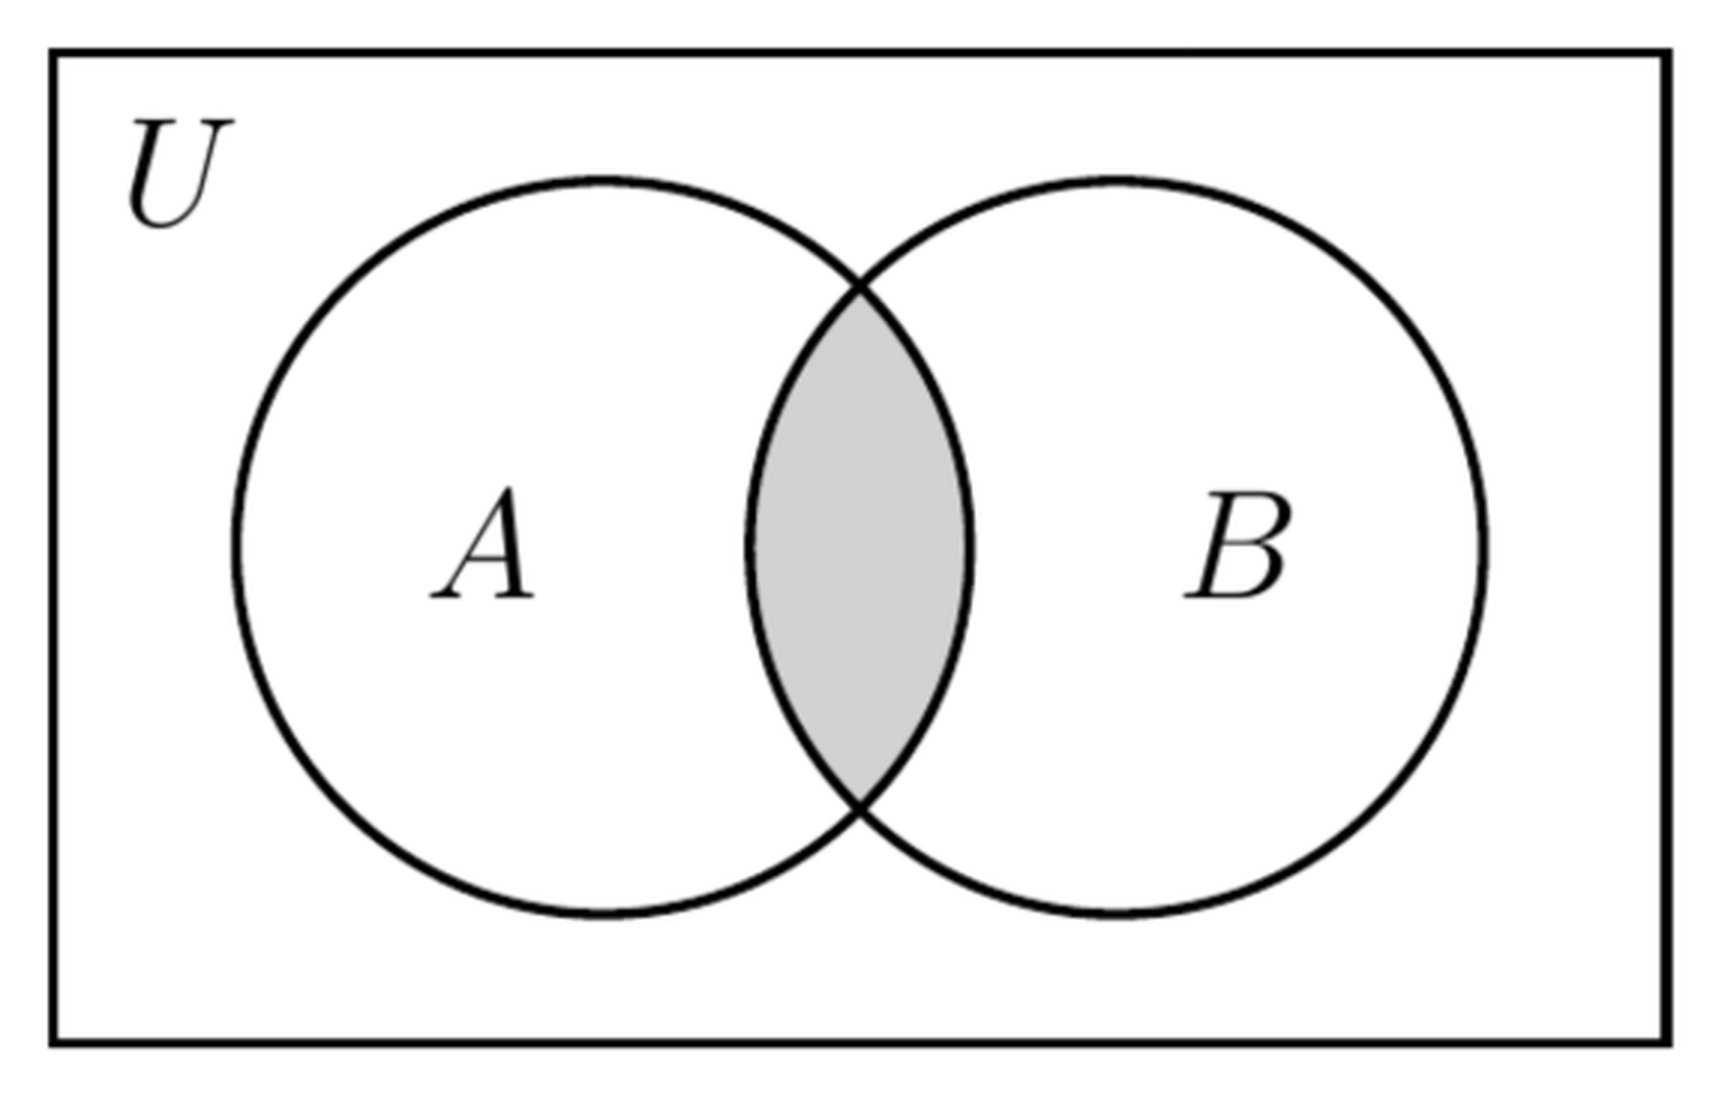
\includegraphics[width=0.38\textwidth]{figures/gao141_q5.png}
\end{center}

\ifanswer
\solbegin
\step{阴影部分表示 $A\cap B=\{4,7\}$.}
\solend
\fi

\item 方程 $2^{\log_3 x}=\dfrac12$ 的解集为\blankline[4.4em].

\ifanswer
\solbegin
\step{$2^{\log_3 x}=2^{-1}\Leftrightarrow\log_3 x=-1\Leftrightarrow x=\dfrac13$，解集为 $\left\{\dfrac13\right\}$.}
\solend
\fi

\item 若集合 $A=\left\{x\mid x^2+ax+\dfrac14=0\right\}$ 有且仅有两个子集，则实数 $a$ 的值为\blankline[4.4em].

\ifanswer
\solbegin
\step{$A$ 有且仅有两个子集，说明 $A$ 恰有一个元素，即方程有两个相等的实数根.}
\step{$\Delta=a^2-4\cdot\dfrac14=0\Rightarrow a=\pm1$.}% 判别式原卷印等腰偏高的高三角 $\Delta$，照录
\solend
\fi

\item 已知关于 $x$ 的方程 $x^2+mx+2m=0$ 的两个实数根分别为 $\alpha$、$\beta$，若 $\alpha^2+\beta^2=5$，则实数 $m=$\blankline[4.4em].

\ifanswer
\solbegin
\step{方程 $x^2+mx+2m=0$ 的两个实数根为 $\alpha$、$\beta$，}
\step{由根与系数的关系得 $\begin{cases}\alpha+\beta=-m\\\alpha\beta=2m\end{cases}$，又因为 $\alpha^2+\beta^2=5$，}
\step{所以 $\alpha^2+\beta^2=(\alpha+\beta)^2-2\alpha\beta=m^2-4m=5$，整理得 $m^2-4m-5=0$，}
\step{解得 $m=5$ 或 $m=-1$，}
\step{当 $m=5$ 时，$\triangle=25-40=-15<0$，无实根，舍去；}% 判别式原卷印扁等边三角 $\triangle$，照录
\step{当 $m=-1$ 时，$\triangle=1+8=9>0$，符合题意，}
\step{所以实数 $m=-1$.}
\solend
\fi

\item 若不等式 $\lvert x-3\rvert+\lvert x-5\rvert\geqslant a$ 对任意的实数 $x$ 恒成立，则实数 $a$ 的取值范围为\blankline[4.4em].

\ifanswer
\solbegin
\step{由三角不等式得 $\lvert x-3\rvert+\lvert x-5\rvert\geqslant\lvert x-3-x+5\rvert=2$，则 $a\leqslant2$.}
\solend
\fi

\item 设集合 $A=\{-3,2\}$，集合 $B=\{x\mid mx+1=0\}$，若 $A\cup B=A$，则实数 $m$ 的值为\blankline[4.4em].

\ifanswer
\solbegin
\step{由 $A\cup B=A$，得 $B\subseteq A$，}% 子集符号原卷印带下划线的 $\subseteq$，照录
\step{当 $m=0$ 时，$B=\varnothing$，满足题意，}
\step{当 $m\neq0$ 时，$B=\left\{-\dfrac1m\right\}$，所以 $-\dfrac1m=2$ 或 $-\dfrac1m=-3$，所以 $m=-\dfrac12$ 或 $m=\dfrac13$，}
\step{综上所述，$m=0$ 或 $m=-\dfrac12$ 或 $m=\dfrac13$.}
\solend
\fi

\item 已知 $m$ 为实数，代数式 $M=\sqrt{m-1}+\sqrt{3-m}$ 的取值范围为\blankline[4.4em].

\ifanswer
\solbegin
\step{根式有意义要求 $m\in[1,3]$，}
\step{此时 $(m-1)(3-m)=1-(m-2)^2$ 的取值范围为 $[0,1]$.}
\step{$M^2=2+2\sqrt{(m-1)(3-m)}$ 的取值范围为 $[2,4]$，又 $M>0$，}
\step{所以 $M\in[\sqrt2,2]$.}
\solend
\fi

\item 设有限集 $M$ 所含元素的个数用 $\mathbf{card}(M)$ 表示，并规定 $\mathbf{card}(\varnothing)=0$. 已知集合 $A,B$ 满足 $A\cup B=\{1,2,3\}$，$A\cap B=\varnothing$，若 $\mathbf{card}(A)\notin A$，$\mathbf{card}(B)\notin B$，则满足条件的所有不同集合 $A$ 的个数为\blankline[4.4em].

\ifanswer
\solbegin
\step{当 $\mathbf{card}(A)=0$ 或 $3$ 时，$A,B$ 中有一个为 $\{1,2,3\}$，不符合条件.}
\step{当 $\mathbf{card}(A)=1$ 时，$\mathbf{card}(B)=2\notin B$，所以 $A=\{2\}$，符合条件.}
\step{当 $\mathbf{card}(A)=2$ 时，$2\notin A$，所以 $B=\{2\}$，$A=\{1,3\}$，符合条件.}
\step{满足条件的集合 $A$ 共 $2$ 个.}
\solend
\fi

\end{enumerate}

\bigsec{二、选择题}

\begin{enumerate}
\setcounter{enumi}{12}

\item “ $x=1$ ” 是 “ $x^2-3x+2=0$ ” 的\mbox{（\quad）}条件.

\keepwithprev
A. 充分非必要\qquad B. 必要非充分

C. 充要\qquad D. 既非充分又非必要

\ifanswer
\solbegin
\step{$x^2-3x+2=0\Leftrightarrow x=1$ 或 $x=2$，所以 “ $x=1$ ” 是其充分非必要条件，}
\step{故选 $A$.}
\solend
\fi

\item 设 $a,b,c\in\R$，则下列命题为真命题的是\mbox{（\quad）}
% 原卷题干只声明 a,b,c，而 A 选项出现未声明的 d，照录（存疑）
\keepwithprev
A. 若 $a>b$ 且 $c>d$，则 $ac>bd$\qquad B. 若 $a^2>b^2$，则 $a>b$

C. 若 $ab>0$ 且 $a>b$，则 $\dfrac1a<\dfrac1b$\qquad D. 若 $a<0<b$，则 $\sqrt{-a}<\sqrt b$

\ifanswer
\solbegin
\step{$ab>0$ 且 $a>b\Rightarrow\dfrac1a-\dfrac1b=\dfrac{b-a}{ab}<0$，所以 $C$ 为真命题，故选 $C$.}
\solend
\fi

\item 已知 $\log_{14}7=a$，$14^b=5$，则 $\log_{35}28=$\mbox{（\quad）}

\keepwithprev
A. $\dfrac{2-a}{2a+b}$\qquad B. $\dfrac{2+a}{a+b}$\qquad C. $\dfrac{2-a}{a+2b}$\qquad D. $\dfrac{2-a}{a+b}$

\ifanswer
\solbegin
\step{$\log_{14}7=a$，$14^b=5$，}
\step{$\log_{35}28=\dfrac{\log_{14}28}{\log_{14}35}=\dfrac{\log_{14}14^2-\log_{14}7}{\log_{14}7+\log_{14}5}=\dfrac{2-a}{a+b}$. 故选 $D$.}
\solend
\fi

\item 关于 $x$ 的不等式 $ax^2+bx+3>0$ 的解集有下列说法，其中正确的个数是\mbox{（\quad）}

\keepwithprev
① 不等式 $ax^2+bx+3>0$ 的解集可以是 $\R$

② 不等式 $ax^2+bx+3>0$ 的解集可以是 $\{x\mid x>3\}$

③ 不等式 $ax^2+bx+3>0$ 的解集可以是 $\varnothing$

④ 不等式 $ax^2+bx+3>0$ 的解集可以是 $\{x\mid -1<x<3\}$

\keepwithprev
A. 4\qquad B. 3\qquad C. 2\qquad D. 1

\ifanswer
\solbegin
\step{$x=0$ 时左端为 $3>0$，解集必含 $0$，所以②③错误.}
\step{①取 $a=1,b=0$，$x^2+3>0$ 的解集为 $\R$，正确.}
\step{④取 $a=-1,b=2$，$-x^2+2x+3=-(x+1)(x-3)>0\Leftrightarrow-1<x<3$，正确.}
\step{正确的有①④，共 $2$ 个，故选 $C$.}
\solend
\fi

\end{enumerate}

\bigsec{三、解答题}

\begin{enumerate}
\setcounter{enumi}{16}

\item 已知集合 $A=\left\{x\mid\dfrac{x-2}{x+3}\geqslant0\right\}$，集合 $B=\{x\mid\lvert x+1\rvert+\lvert x-1\rvert<5\}$，全集 $U=\R$.

(1) 求 $A,B$；

(2) 求 $A\cup B$、$\overline{A\cap B}$.

\ifanswer
\solbegin
\step{(1) 分母不为零，且分子、分母同号或分子为零，}
\step{所以 $\dfrac{x-2}{x+3}\geqslant0\Leftrightarrow x<-3$ 或 $x\geqslant2$，因此 $A=(-\infty,-3)\cup[2,+\infty)$.}
\step{又 $\lvert x+1\rvert+\lvert x-1\rvert=\begin{cases}-2x,&x<-1\\2,&-1\leqslant x\leqslant1\\2x,&x>1\end{cases}$，}
\step{分别解得 $-\dfrac52<x<-1$、$-1\leqslant x\leqslant1$、$1<x<\dfrac52$，因此 $B=\left(-\dfrac52,\dfrac52\right)$.}
\step{(2) 合并两集合所对应的区间，得 $A\cup B=(-\infty,-3)\cup\left(-\dfrac52,+\infty\right)$，}
\step{两集合的公共部分为 $A\cap B=\left[2,\dfrac52\right)$，所以 $\overline{A\cap B}=(-\infty,2)\cup\left[\dfrac52,+\infty\right)$.}
\solend
\fi

\item (1) 已知 $a>b>0$，比较代数式 $\dfrac ab$ 与 $\dfrac{a+1}{b+1}$ 的大小并说明理由；

(2) 已知 $x,y,z$ 都是正实数，$a=x+\dfrac1y,b=y+\dfrac1z,c=z+\dfrac1x$，试用反证法证明 $a,b,c$ 至少有一个不小于 $2$.

\ifanswer
\solbegin
\step{(1) $\dfrac ab-\dfrac{a+1}{b+1}=\dfrac{a(b+1)-b(a+1)}{b(b+1)}=\dfrac{a-b}{b(b+1)}$，}
\step{因为 $a>b>0$，所以 $a-b>0$，$b(b+1)>0$，所以 $\dfrac ab-\dfrac{a+1}{b+1}>0$，}
\step{故 $\dfrac ab>\dfrac{a+1}{b+1}$.}
\step{(2) 假设 $a$、$b$、$c$ 三数都小于 $2$，则 $x+\dfrac1y+y+\dfrac1z+z+\dfrac1x<6$.}
\step{因为 $x,y,z$ 均大于 $0$，}
\step{所以 $x+\dfrac1y+y+\dfrac1z+z+\dfrac1x=x+\dfrac1x+y+\dfrac1y+z+\dfrac1z\geqslant2+2+2=6$，矛盾，}
\step{所以 $a$、$b$、$c$ 三数中至少有一个不小于 $2$.}
\solend
\fi

% 第 19 题长方体无盖贮水池砖墙示意图（题目配图，三版都出）：取原卷 06 页截图去粉色水印、LANCZOS 放大 3 倍
\needvspace{6cm}
\item 如图所示，某工厂要建造一个长方体形无盖贮水池，其容积为 $3200m^3$，深为 $2m$.

(1) 若水池的长比宽至少多 $60m$，求水池的宽的最大值；

(2) 若池底每平方米的造价为 $150$ 元，池壁每平方米的造价为 $120$ 元，那么怎样设计水池的长和宽能使总造价最低？最低总造价是多少？

\begin{center}
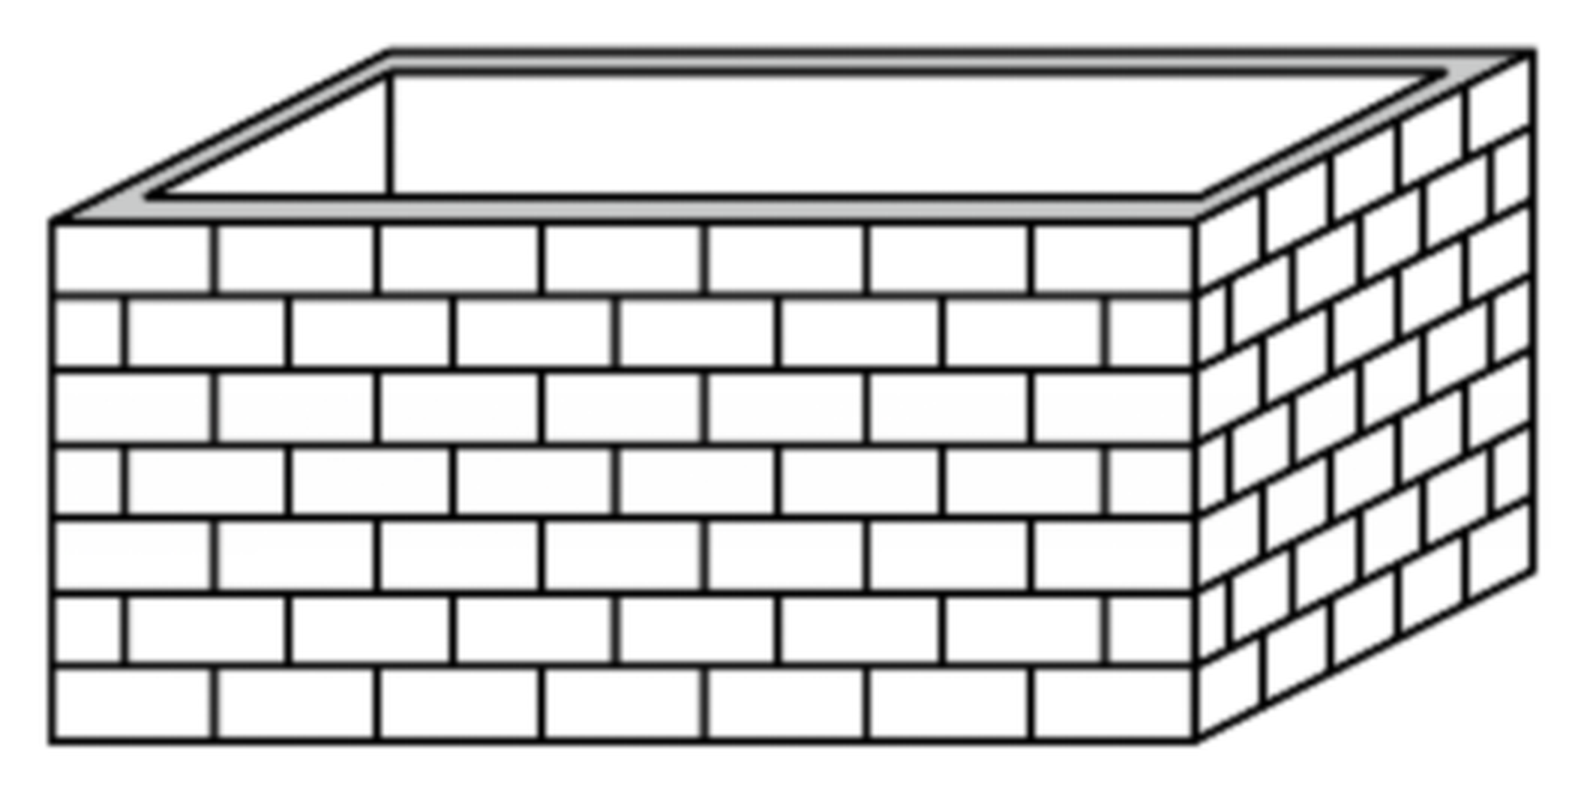
\includegraphics[width=0.42\textwidth]{figures/gao141_q19.png}
\end{center}

\ifanswer
\solbegin
\step{(1) 设水池的长、宽分别为 $xm$，$ym$，则 $x-y\geqslant60$，且 $x$、$y>0$，}
\step{由题意得 $2xy=3200$，即 $x=\dfrac{1600}{y}$，所以 $\dfrac{1600}{y}-y\geqslant60$，}
\step{因为 $y>0$，所以 $1600-y^2\geqslant60y$，}
\step{即 $y^2+60y-1600=(y+80)(y-20)\leqslant0$，解得 $-80\leqslant y\leqslant20$，}
\step{又 $y>0$，所以 $0<y\leqslant20$，所以水池的宽的最大值为 $20m$.}
\step{(2) 设水池总造价为 $z$ 元，}
\step{则 $z=1600\times150+2\times(2x+2y)\times120=240000+480(x+y)$，}
\step{又因为 $y=\dfrac{1600}{x}$，}
\step{所以 $z=240000+\left(x+\dfrac{1600}{x}\right)\times480\geqslant240000+480\times2\sqrt{1600}$}
\step{$=240000+38400=278400$，}
\step{当且仅当 $x=\dfrac{1600}{x}$，即 $x=y=40$ 时取等号，}
\step{所以，将水池的池底设计为边长为 $40m$ 的正方形时总造价最低，}
\step{最低总造价为 $278400$ 元.}
\solend
\fi

\item 已知 $a\in\R$，设集合 $A=\{x\mid ax^2-3x+2<ax-1\}$.

(1) 若 $A=(1,3)$，求实数 $a$ 的值；

(2) 当 $a>0$ 时，求 $A$；

(3) 若 “ $x\in\left(\dfrac12,+\infty\right)$ ” 是 “ $x\in A$ ” 的必要非充分条件，求实数 $a$ 的取值范围.

\ifanswer
\solbegin
\step{原不等式等价于 $ax^2-(a+3)x+3<0\Leftrightarrow(x-1)(ax-3)<0$，}
\step{(1) $A=(1,3)$ 为有界区间，因此 $a>0$，两根为 $1$ 和 $\dfrac3a$，于是 $\dfrac3a=3$，得 $a=1$；}
\step{此时 $(x-1)(x-3)<0$ 的解集确为 $(1,3)$.}
\step{(2) 当 $a>0$ 时，二次项系数为正，比较 $1$ 与 $\dfrac3a$，得 $A=\begin{cases}\left(1,\dfrac3a\right),&0<a<3\\\varnothing,&a=3\\\left(\dfrac3a,1\right),&a>3\end{cases}$，}
\step{其中 $a=3$ 时，原不等式为 $3(x-1)^2<0$，无解.}
\step{(3) 记 $S=\left(\dfrac12,+\infty\right)$，题意要求 $A\subset S$.}% 子集符号原卷印单线 $\subset$，照录
\step{由于对任意 $a$ 都有 $1\notin A$，而 $1\in S$，所以只需满足 $A\subseteq S$.}
\step{当 $a<0$ 时，$A=\left(-\infty,\dfrac3a\right)\cup(1,+\infty)$，含有小于 $\dfrac12$ 的数，不符合条件.}
\step{当 $a=0$ 时，$A=(1,+\infty)$，符合条件.}
\step{当 $0<a<3$ 时，$A=\left(1,\dfrac3a\right)\subseteq S$；}
\step{当 $a=3$ 时，$A=\varnothing\subseteq S$，均符合条件；}
\step{当 $a>3$ 时，$A=\left(\dfrac3a,1\right)$，所以 $A\subseteq S\Leftrightarrow\dfrac3a\geqslant\dfrac12\Leftrightarrow a\leqslant6$；}
\step{因此实数 $a$ 的取值范围为 $[0,6]$.}
\solend
\fi

\item 甲、乙两同学探讨了一个问题：已知正实数 $x,y$ 满足 $3x+y=1$，求 $\dfrac1x+\dfrac1y$ 的最小值.

甲给出的解法：由 $1=3x+y\geqslant2\sqrt{3xy}$，得 $\sqrt{xy}\leqslant\dfrac{\sqrt3}{6}$，所以 $\dfrac1x+\dfrac1y\geqslant2\sqrt{\dfrac1{xy}}\geqslant4\sqrt3$. 因此 $\dfrac1x+\dfrac1y$ 的最小值为 $4\sqrt3$.

乙给出的解法：$\dfrac1x+\dfrac1y=\left(\dfrac1x+\dfrac1y\right)(3x+y)=4+\dfrac yx+\dfrac{3x}{y}$，因为 $x,y$ 均为正实数，所以 $\dfrac1x+\dfrac1y\geqslant4+2\sqrt{\dfrac yx\cdot\dfrac{3x}{y}}=4+2\sqrt3$.

(1) 请判断上述哪位同学的解法正确，哪位同学的解法错误，并指出错误的原因；

(2) 结合上述探讨，试求当 $0<x<\dfrac12$ 时，$\dfrac1x+\dfrac1{1-2x}$ 的最小值以及此时实数 $x$ 的值；

(3) 已知 $x$ 为正实数，$y$ 为非负实数，且 $x+2y=2$，求 $\dfrac{x^2+1}{x}+\dfrac{2y^2}{y+1}$ 的最小值以及此时实数 $x,y$ 的值.

\ifanswer
\solbegin
\step{(1) 甲的推导中，$3x+y\geqslant2\sqrt{3xy}$ 取等号要求 $3x=y$，}
\step{$\dfrac1x+\dfrac1y\geqslant\dfrac2{\sqrt{xy}}$ 取等号要求 $x=y$，两者对正实数 $x,y$ 不能同时成立，}
\step{因此不能将 $4\sqrt3$ 判为最小值，甲错误.}
\step{乙的等号条件为 $\dfrac yx=\dfrac{3x}{y}$，即 $y=\sqrt3 x$；}
\step{结合 $3x+y=1$，得 $x=\dfrac1{3+\sqrt3},y=\dfrac{\sqrt3}{3+\sqrt3}$ 均为正数，等号可以成立，}
\step{因此乙正确，最小值为 $4+2\sqrt3$.}
\step{(2) 令 $t=1-2x>0$，则 $2x+t=1$.}
\step{$\dfrac1x+\dfrac1t=\left(\dfrac1x+\dfrac1t\right)(2x+t)=3+\dfrac tx+\dfrac{2x}{t}\geqslant3+2\sqrt2$，}
\step{当且仅当 $\dfrac tx=\dfrac{2x}{t}$，即 $t=\sqrt2 x$ 时取等号，}
\step{由 $2x+t=1$，得 $x=\dfrac1{2+\sqrt2}=\dfrac{2-\sqrt2}{2}\in\left(0,\dfrac12\right)$，}
\step{因此最小值为 $3+2\sqrt2$，此时 $x=\dfrac{2-\sqrt2}{2}$.}
\step{(3) 记目标式为 $F$，利用 $x+2y=2$，}
\step{得 $F=x+\dfrac1x+2y-2+\dfrac2{y+1}=\dfrac1x+\dfrac2{y+1}$，}
\step{又 $x+2(y+1)=4$，且 $x>0$、$y+1>0$，}
\step{所以 $4F=\left(\dfrac1x+\dfrac2{y+1}\right)(x+2(y+1))=5+2\left(\dfrac{y+1}{x}+\dfrac{x}{y+1}\right)$}
\step{$\geqslant5+2\times2=9$，当且仅当 $\dfrac{y+1}{x}=\dfrac{x}{y+1}$，即 $x=y+1$ 时取等号.}
\step{联立 $x+2y=2$，得 $x=\dfrac43$、$y=\dfrac13$，满足题设条件，}
\step{因此最小值为 $\dfrac94$，此时 $x=\dfrac43$，$y=\dfrac13$.}
\solend
\fi

\end{enumerate}

\end{document}
"
%
% ① 原始材料：微信公众号"魔都数学加油站"文章，连载"27学年高一141"，原文标题
% "27学年高一141——2026-2027年上海市彭浦中学高一上期中"；
% 原文链接：https://mp.weixin.qq.com/s/V_8bEhC6geeFyQysmtqUtQ。
% 正文为 9 张 PNG 页（01、05、06、07、09 为 2560x3620；02、03、04、08 为 4762x6735，
% 同一篇各页分辨率不同，逐页按各自分辨率放大裁图核对），题目下印【解析】，为讲评版。
% 题目、解析均据原图转录；卷面粉红色水印"魔都数学加油站"及公众号页脚未录入。
% 全卷 2 幅插图，均属题目配图（在 \ifanswer 外、三版都出）、取原卷截图去粉色水印、
% LANCZOS 放大 3 倍：第 5 题韦恩图（01 页，全集 U 矩形内两圆相交、交集阴影、A/B/U 标注）、
% 第 19 题长方体无盖贮水池砖墙示意图（06 页右上）。通读 9 页确认除这 2 幅外无其它
% 插图/表格，亦无"题干写如图而源码漏图"（仅 Q5"图中阴影部分"、Q19"如图所示"两处提到图）。
%
% 卷首标题：原卷印作"2026-2027 年彭浦中学高一上期中"（公众号标题中的"上海市"
% 卷面标题行没有，本稿照卷面），年份区间按全稿惯例排 en dash；原卷未印副标题，
% 本卷为期中卷、跨集合与常用逻辑用语／不等式／函数三章，按题目内容补出
% "集合与常用逻辑用语、不等式、函数"（与 高一140 同期中卷口径相同）：
% 集合与逻辑见 Q5、Q10、Q12、Q13、Q16、Q17、Q20，不等式见 Q4、Q9、Q14、Q18、
% Q19、Q21，函数（指数／对数）见 Q6、Q15。
%
% 题号体例：本卷共 19 题——一、填空题 3—12（10 题）、二、选择题 13—16（4 题）、
% 三、解答题 17—21（5 题）。三节分别 \setcounter{enumi}{2}／{12}／{16}。
% 原卷从第 3 题起、无第 1、2 题，本稿保留原题号；全卷无附加题节。
%
% ② 与原卷的排版差异：
%   ① 原文从第 3 题起，本稿保留原题号；
%   ② 原卷 19 题题下均印【解析】，无独立【答案】段、无"答案印题干括号且无解析"、
%      无"只印【答案】无解析"一型：填空题与解答题的答案落在【解析】末句
%      （Q3—Q12、Q17—Q21），四道选择题答案在【解析】末句"故选 …"
%      （Q13 选 A、Q14 选 C、Q15 选 D、Q16 选 C），题干括号内一律留空；
%      本稿 19 题一律 \solbegin…\solend、全卷不提 \ans{}，答案版【解析】标记数
%      = 19 = 全卷题数（无【答案】标记）；
%   ③ 原卷未印副标题，本稿按"知识模块"口径补出；
%   ④ 原卷填空横线按全稿惯例排 \blankline[4.4em]；选择题括号排 \mbox{（\quad）}，
%      选项段／命题段前按惯例加 \keepwithprev（Q16 两枚：命题列与选项段各一）；
%      解答题不留作答区、不加 \anspace（原卷为讲评版，与 129／131／132／133／136／140 同）；
%   ⑤ 原卷数集混排：黑板粗体 R（Q14 题干、Q16 ① 与解析、Q17 全集、Q20 题干）
%      按全稿惯例统一改 \R；空集记号 \varnothing；绝对值排 \lvert…\rvert，
%      集合描述竖线排 \mid；不等号按全稿惯例排 \leqslant／\geqslant；
%      补集照原卷上划线排 \overline{A\cap B}（Q17(2) 题干与解析）；
%      原卷"card"记号排黑体正体（Q12），本稿照录 \mathbf{card}，未改斜体
%      （与 高一66 同题口径不同：那份原卷 card 排斜体、照录 $card(M)$）；
%   ⑥ 子题标号 (1)(2)(3) 原卷印半角括号，照录；圈数字 ①②③④ 在正文（文本模式）
%      按原卷照录，未进数学式；数学式内半角逗号照录（如 Q12"$A,B$"、"{1,2,3}"、
%      Q14"$a,b,c\in\R$"、Q15"$\log_{14}7=a$，$14^b=5$"、Q16"$a=1,b=0$"、
%      Q18"$x,y,z$"、Q20"$x,y$"、Q21"$x,y$"）；全卷行末西文句点照录为 ASCII 句点；
%      行中全角逗号、顿号照录；
%   ⑦ 题干中的中文弯引号按原卷照录（Q13、Q20(3) 的 “ ” 及引号内空格），
%      注释内一律 ASCII 引号；
%   ⑧ 两幅题目配图各在 \item 之前加 \needvspace 守卫整块推走（Q5 5cm、Q19 6cm），
%      守卫放在 \item 之前而非 \bigsec 之后——两题均非各节首题，不触发 B 类
%      "节标题落页末"（照 高一26／40／59／136／140 成例）；三版切页审计均"合计异常：无"；
%   ⑨ 跨页续印按题合并：Q8 题干与【解析】首行在 01 页、后 6 行在 02 页；
%      Q15 题干在 03 页、【解析】在 04 页；Q17 题干与【解析】前 2 行在 04 页、
%      后 4 行在 05 页；Q19 题干在 05 页末、(1)(2) 小问与砖墙图与【解析】在 06 页；
%      Q20 题干 (1)(2) 在 06 页末、(3) 与【解析】在 07 页；Q21 题干与【解析】
%      前 6 行在 08 页、后 12 行在 09 页；Q16、Q18 全在各自页内；
%      本稿按题连排，不丢行；
%   ⑩ 原卷无红色加粗标签（【解析】均黑色印刷，Q16 解析 "①取…""④取…" 与
%      Q20 解析 "(2)" 等分步标签亦黑色），故本卷未用 \stepm；
%   ⑪ 原卷 Q19 题干把数值与单位（3200m³、2m、60m、150 元、120 元、40m、20m、
%      278400 元）印作略粗的西文字形，本稿按全稿惯例（高一70／72 同类题）排普通
%      数学体，未加粗。
%
% ③ 行数复核：一条 \step = 原卷解析的一个印刷行，cases 块作一个印刷行计。逐题数 \step
%   条数，合计 92 条（Q3：1；Q4：1；Q5：1；Q6：1；Q7：2；Q8：7；Q9：1；Q10：4；
%   Q11：4；Q12：4；Q13：2；Q14：1；Q15：2；Q16：4；Q17：6；Q18：7；Q19：13；
%   Q20：13；Q21：18），与原卷印刷行逐题相等。全卷 19 题均印【解析】、无独立 \ans{}，
%   答案版【解析】标记数 = 19 = 全卷题数。
%
% ④ 判别式／子集符号结论（逐处放大原图照录、不得统一）：
%   判别式：全卷 3 处——第 7 题【解析】"$\Delta=a^2-4\cdot\frac14=0$"一处原卷印
%     等腰、偏高的高三角 $\Delta$，照录 \Delta；第 8 题【解析】
%     "$\triangle=25-40=-15<0$"与"$\triangle=1+8=9>0$"两处原卷印扁等边三角
%     $\triangle$，照录 \triangle。两形不同，逐处照录未统一。
%   子集：全卷 6 处——第 10 题【解析】"$B\subseteq A$"一处、第 20 题【解析】
%     "所以只需满足 $A\subseteq S$"、"$A=\left(1,\frac3a\right)\subseteq S$"、
%     "$A=\varnothing\subseteq S$"、"$A\subseteq S\Leftrightarrow\frac3a\geqslant\frac12$"
%     四处，共 5 处原卷印带下划线的 $\subseteq$，照录 \subseteq；第 20 题【解析】
%     (3) 首行"题意要求 $A\subset S$"一处原卷印单线 $\subset$，照录 \subset
%     （下行因 $1\in S$ 而 $1\notin A$，改述为 $A\subseteq S$，两者逻辑一致、非笔误）。
%
% ⑤ 存疑照录（照录未改，正文对应处另有 % 注）：
%   第 14 题题干"设 $a,b,c\in\R$"只声明 $a,b,c$，而 A 选项"若 $a>b$ 且 $c>d$，
%     则 $ac>bd$"引入未声明的 $d$，原卷变量声明与选项不统一，照录未补。
%   全卷除此 1 条外未发现其它笔误／自相矛盾处。
%
% ⑥ 跨页续印按题合并说明：见 ② ⑨。
%
\documentclass[a4paper,11pt]{article}
\usepackage{common}

\begin{document}

\examtitlest[3]{2026--2027 年彭浦中学高一上期中}{集合与常用逻辑用语、不等式、函数}

\bigsec{一、填空题}

\begin{enumerate}
\setcounter{enumi}{2}

\item 已知 $m$ 为实数，若 $1\in\{m,m^2\}$，则 $m$ 的值为\blankline[4.4em].

\ifanswer
\solbegin
\step{$m=1$ 或 $m^2=1$，得 $m=\pm1$；按列举项互异口径排除 $m=m^2=1$，得 $m=-1$.}
\solend
\fi

\item 已知 $2<a<4$，$-2<b<1$，则 $2a+b$ 的取值范围为\blankline[4.4em].

\ifanswer
\solbegin
\step{$4<2a<8$，与 $-2<b<1$ 相加，得 $2<2a+b<9$，取值范围为 $(2,9)$.}
\solend
\fi

% 第 5 题韦恩图（题目配图，三版都出）：取原卷 01 页截图去粉色水印、LANCZOS 放大 3 倍
\needvspace{5cm}
\item 已知集合 $A=\{-1,-2,1,4,7\}$，$B=\{x\mid x>1\}$，用列举法表示图中阴影部分所表示的集合为\blankline[4.4em].

\begin{center}
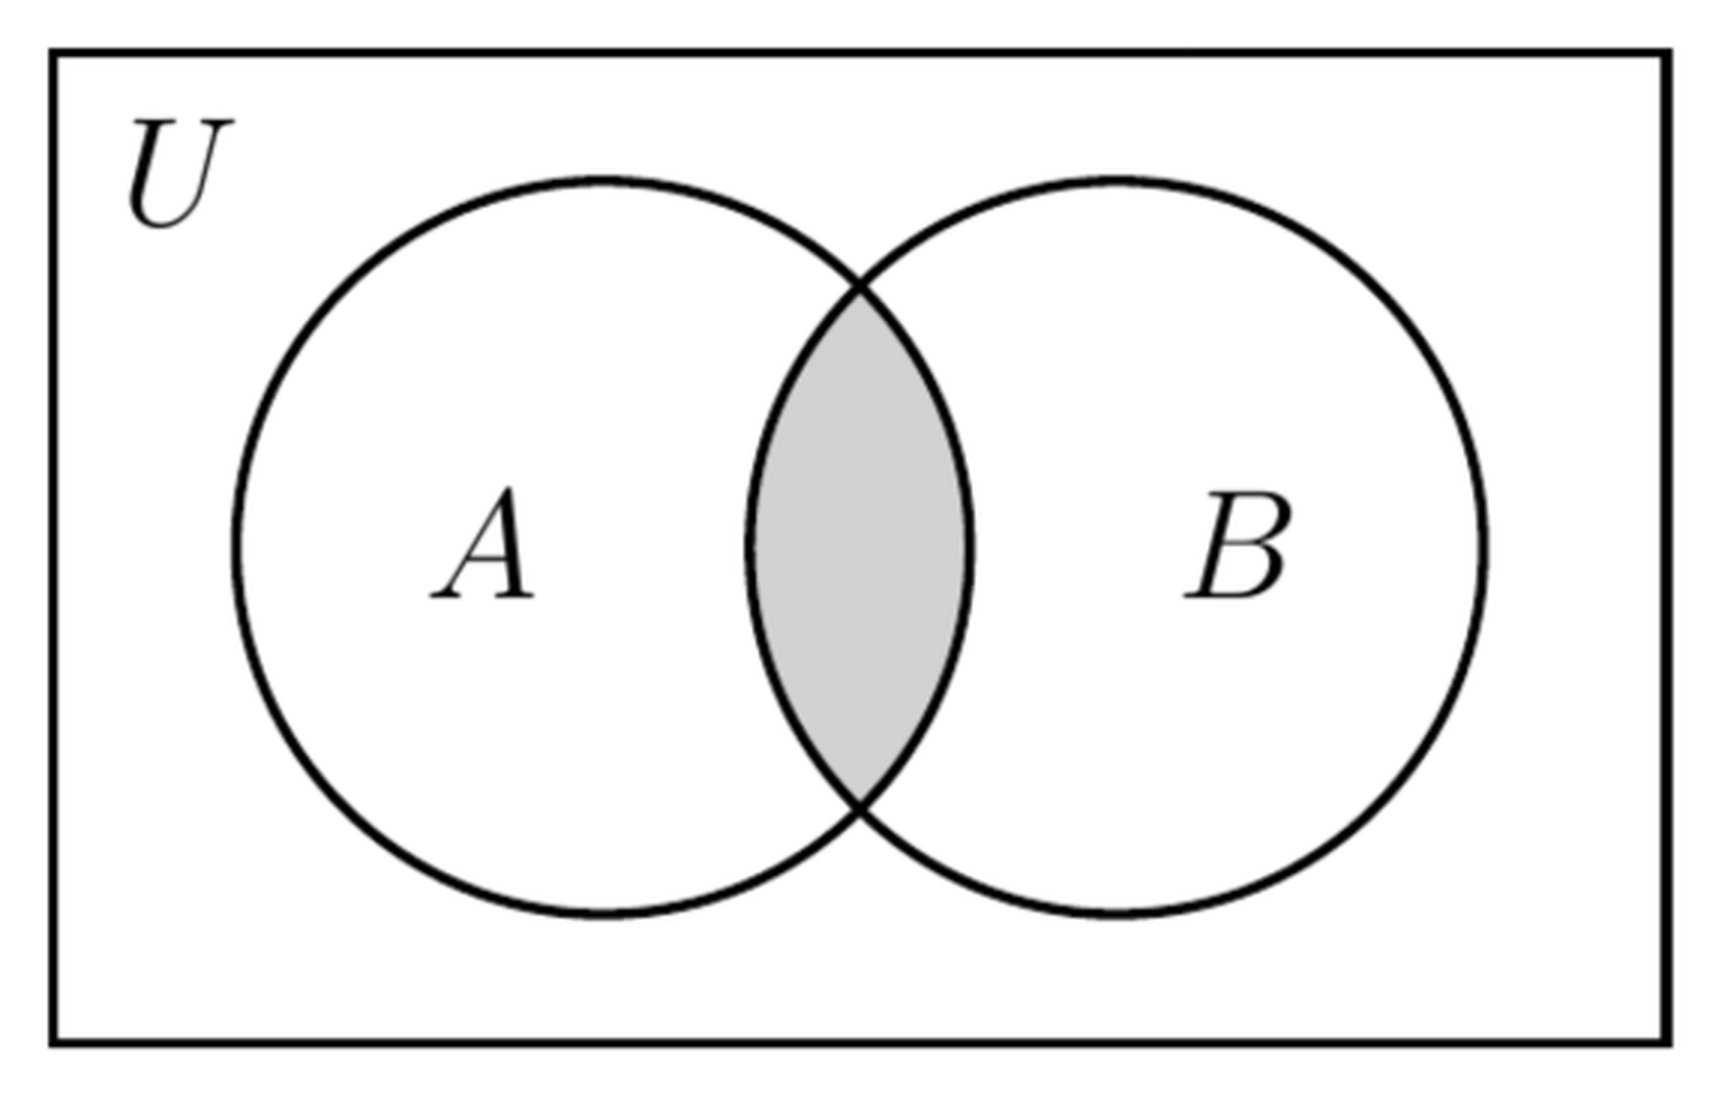
\includegraphics[width=0.38\textwidth]{figures/gao141_q5.png}
\end{center}

\ifanswer
\solbegin
\step{阴影部分表示 $A\cap B=\{4,7\}$.}
\solend
\fi

\item 方程 $2^{\log_3 x}=\dfrac12$ 的解集为\blankline[4.4em].

\ifanswer
\solbegin
\step{$2^{\log_3 x}=2^{-1}\Leftrightarrow\log_3 x=-1\Leftrightarrow x=\dfrac13$，解集为 $\left\{\dfrac13\right\}$.}
\solend
\fi

\item 若集合 $A=\left\{x\mid x^2+ax+\dfrac14=0\right\}$ 有且仅有两个子集，则实数 $a$ 的值为\blankline[4.4em].

\ifanswer
\solbegin
\step{$A$ 有且仅有两个子集，说明 $A$ 恰有一个元素，即方程有两个相等的实数根.}
\step{$\Delta=a^2-4\cdot\dfrac14=0\Rightarrow a=\pm1$.}% 判别式原卷印等腰偏高的高三角 $\Delta$，照录
\solend
\fi

\item 已知关于 $x$ 的方程 $x^2+mx+2m=0$ 的两个实数根分别为 $\alpha$、$\beta$，若 $\alpha^2+\beta^2=5$，则实数 $m=$\blankline[4.4em].

\ifanswer
\solbegin
\step{方程 $x^2+mx+2m=0$ 的两个实数根为 $\alpha$、$\beta$，}
\step{由根与系数的关系得 $\begin{cases}\alpha+\beta=-m\\\alpha\beta=2m\end{cases}$，又因为 $\alpha^2+\beta^2=5$，}
\step{所以 $\alpha^2+\beta^2=(\alpha+\beta)^2-2\alpha\beta=m^2-4m=5$，整理得 $m^2-4m-5=0$，}
\step{解得 $m=5$ 或 $m=-1$，}
\step{当 $m=5$ 时，$\triangle=25-40=-15<0$，无实根，舍去；}% 判别式原卷印扁等边三角 $\triangle$，照录
\step{当 $m=-1$ 时，$\triangle=1+8=9>0$，符合题意，}
\step{所以实数 $m=-1$.}
\solend
\fi

\item 若不等式 $\lvert x-3\rvert+\lvert x-5\rvert\geqslant a$ 对任意的实数 $x$ 恒成立，则实数 $a$ 的取值范围为\blankline[4.4em].

\ifanswer
\solbegin
\step{由三角不等式得 $\lvert x-3\rvert+\lvert x-5\rvert\geqslant\lvert x-3-x+5\rvert=2$，则 $a\leqslant2$.}
\solend
\fi

\item 设集合 $A=\{-3,2\}$，集合 $B=\{x\mid mx+1=0\}$，若 $A\cup B=A$，则实数 $m$ 的值为\blankline[4.4em].

\ifanswer
\solbegin
\step{由 $A\cup B=A$，得 $B\subseteq A$，}% 子集符号原卷印带下划线的 $\subseteq$，照录
\step{当 $m=0$ 时，$B=\varnothing$，满足题意，}
\step{当 $m\neq0$ 时，$B=\left\{-\dfrac1m\right\}$，所以 $-\dfrac1m=2$ 或 $-\dfrac1m=-3$，所以 $m=-\dfrac12$ 或 $m=\dfrac13$，}
\step{综上所述，$m=0$ 或 $m=-\dfrac12$ 或 $m=\dfrac13$.}
\solend
\fi

\item 已知 $m$ 为实数，代数式 $M=\sqrt{m-1}+\sqrt{3-m}$ 的取值范围为\blankline[4.4em].

\ifanswer
\solbegin
\step{根式有意义要求 $m\in[1,3]$，}
\step{此时 $(m-1)(3-m)=1-(m-2)^2$ 的取值范围为 $[0,1]$.}
\step{$M^2=2+2\sqrt{(m-1)(3-m)}$ 的取值范围为 $[2,4]$，又 $M>0$，}
\step{所以 $M\in[\sqrt2,2]$.}
\solend
\fi

\item 设有限集 $M$ 所含元素的个数用 $\mathbf{card}(M)$ 表示，并规定 $\mathbf{card}(\varnothing)=0$. 已知集合 $A,B$ 满足 $A\cup B=\{1,2,3\}$，$A\cap B=\varnothing$，若 $\mathbf{card}(A)\notin A$，$\mathbf{card}(B)\notin B$，则满足条件的所有不同集合 $A$ 的个数为\blankline[4.4em].

\ifanswer
\solbegin
\step{当 $\mathbf{card}(A)=0$ 或 $3$ 时，$A,B$ 中有一个为 $\{1,2,3\}$，不符合条件.}
\step{当 $\mathbf{card}(A)=1$ 时，$\mathbf{card}(B)=2\notin B$，所以 $A=\{2\}$，符合条件.}
\step{当 $\mathbf{card}(A)=2$ 时，$2\notin A$，所以 $B=\{2\}$，$A=\{1,3\}$，符合条件.}
\step{满足条件的集合 $A$ 共 $2$ 个.}
\solend
\fi

\end{enumerate}

\bigsec{二、选择题}

\begin{enumerate}
\setcounter{enumi}{12}

\item “ $x=1$ ” 是 “ $x^2-3x+2=0$ ” 的\mbox{（\quad）}条件.

\keepwithprev
A. 充分非必要\qquad B. 必要非充分

C. 充要\qquad D. 既非充分又非必要

\ifanswer
\solbegin
\step{$x^2-3x+2=0\Leftrightarrow x=1$ 或 $x=2$，所以 “ $x=1$ ” 是其充分非必要条件，}
\step{故选 $A$.}
\solend
\fi

\item 设 $a,b,c\in\R$，则下列命题为真命题的是\mbox{（\quad）}
% 原卷题干只声明 a,b,c，而 A 选项出现未声明的 d，照录（存疑）
\keepwithprev
A. 若 $a>b$ 且 $c>d$，则 $ac>bd$\qquad B. 若 $a^2>b^2$，则 $a>b$

C. 若 $ab>0$ 且 $a>b$，则 $\dfrac1a<\dfrac1b$\qquad D. 若 $a<0<b$，则 $\sqrt{-a}<\sqrt b$

\ifanswer
\solbegin
\step{$ab>0$ 且 $a>b\Rightarrow\dfrac1a-\dfrac1b=\dfrac{b-a}{ab}<0$，所以 $C$ 为真命题，故选 $C$.}
\solend
\fi

\item 已知 $\log_{14}7=a$，$14^b=5$，则 $\log_{35}28=$\mbox{（\quad）}

\keepwithprev
A. $\dfrac{2-a}{2a+b}$\qquad B. $\dfrac{2+a}{a+b}$\qquad C. $\dfrac{2-a}{a+2b}$\qquad D. $\dfrac{2-a}{a+b}$

\ifanswer
\solbegin
\step{$\log_{14}7=a$，$14^b=5$，}
\step{$\log_{35}28=\dfrac{\log_{14}28}{\log_{14}35}=\dfrac{\log_{14}14^2-\log_{14}7}{\log_{14}7+\log_{14}5}=\dfrac{2-a}{a+b}$. 故选 $D$.}
\solend
\fi

\item 关于 $x$ 的不等式 $ax^2+bx+3>0$ 的解集有下列说法，其中正确的个数是\mbox{（\quad）}

\keepwithprev
① 不等式 $ax^2+bx+3>0$ 的解集可以是 $\R$

② 不等式 $ax^2+bx+3>0$ 的解集可以是 $\{x\mid x>3\}$

③ 不等式 $ax^2+bx+3>0$ 的解集可以是 $\varnothing$

④ 不等式 $ax^2+bx+3>0$ 的解集可以是 $\{x\mid -1<x<3\}$

\keepwithprev
A. 4\qquad B. 3\qquad C. 2\qquad D. 1

\ifanswer
\solbegin
\step{$x=0$ 时左端为 $3>0$，解集必含 $0$，所以②③错误.}
\step{①取 $a=1,b=0$，$x^2+3>0$ 的解集为 $\R$，正确.}
\step{④取 $a=-1,b=2$，$-x^2+2x+3=-(x+1)(x-3)>0\Leftrightarrow-1<x<3$，正确.}
\step{正确的有①④，共 $2$ 个，故选 $C$.}
\solend
\fi

\end{enumerate}

\bigsec{三、解答题}

\begin{enumerate}
\setcounter{enumi}{16}

\item 已知集合 $A=\left\{x\mid\dfrac{x-2}{x+3}\geqslant0\right\}$，集合 $B=\{x\mid\lvert x+1\rvert+\lvert x-1\rvert<5\}$，全集 $U=\R$.

(1) 求 $A,B$；

(2) 求 $A\cup B$、$\overline{A\cap B}$.

\ifanswer
\solbegin
\step{(1) 分母不为零，且分子、分母同号或分子为零，}
\step{所以 $\dfrac{x-2}{x+3}\geqslant0\Leftrightarrow x<-3$ 或 $x\geqslant2$，因此 $A=(-\infty,-3)\cup[2,+\infty)$.}
\step{又 $\lvert x+1\rvert+\lvert x-1\rvert=\begin{cases}-2x,&x<-1\\2,&-1\leqslant x\leqslant1\\2x,&x>1\end{cases}$，}
\step{分别解得 $-\dfrac52<x<-1$、$-1\leqslant x\leqslant1$、$1<x<\dfrac52$，因此 $B=\left(-\dfrac52,\dfrac52\right)$.}
\step{(2) 合并两集合所对应的区间，得 $A\cup B=(-\infty,-3)\cup\left(-\dfrac52,+\infty\right)$，}
\step{两集合的公共部分为 $A\cap B=\left[2,\dfrac52\right)$，所以 $\overline{A\cap B}=(-\infty,2)\cup\left[\dfrac52,+\infty\right)$.}
\solend
\fi

\item (1) 已知 $a>b>0$，比较代数式 $\dfrac ab$ 与 $\dfrac{a+1}{b+1}$ 的大小并说明理由；

(2) 已知 $x,y,z$ 都是正实数，$a=x+\dfrac1y,b=y+\dfrac1z,c=z+\dfrac1x$，试用反证法证明 $a,b,c$ 至少有一个不小于 $2$.

\ifanswer
\solbegin
\step{(1) $\dfrac ab-\dfrac{a+1}{b+1}=\dfrac{a(b+1)-b(a+1)}{b(b+1)}=\dfrac{a-b}{b(b+1)}$，}
\step{因为 $a>b>0$，所以 $a-b>0$，$b(b+1)>0$，所以 $\dfrac ab-\dfrac{a+1}{b+1}>0$，}
\step{故 $\dfrac ab>\dfrac{a+1}{b+1}$.}
\step{(2) 假设 $a$、$b$、$c$ 三数都小于 $2$，则 $x+\dfrac1y+y+\dfrac1z+z+\dfrac1x<6$.}
\step{因为 $x,y,z$ 均大于 $0$，}
\step{所以 $x+\dfrac1y+y+\dfrac1z+z+\dfrac1x=x+\dfrac1x+y+\dfrac1y+z+\dfrac1z\geqslant2+2+2=6$，矛盾，}
\step{所以 $a$、$b$、$c$ 三数中至少有一个不小于 $2$.}
\solend
\fi

% 第 19 题长方体无盖贮水池砖墙示意图（题目配图，三版都出）：取原卷 06 页截图去粉色水印、LANCZOS 放大 3 倍
\needvspace{6cm}
\item 如图所示，某工厂要建造一个长方体形无盖贮水池，其容积为 $3200m^3$，深为 $2m$.

(1) 若水池的长比宽至少多 $60m$，求水池的宽的最大值；

(2) 若池底每平方米的造价为 $150$ 元，池壁每平方米的造价为 $120$ 元，那么怎样设计水池的长和宽能使总造价最低？最低总造价是多少？

\begin{center}
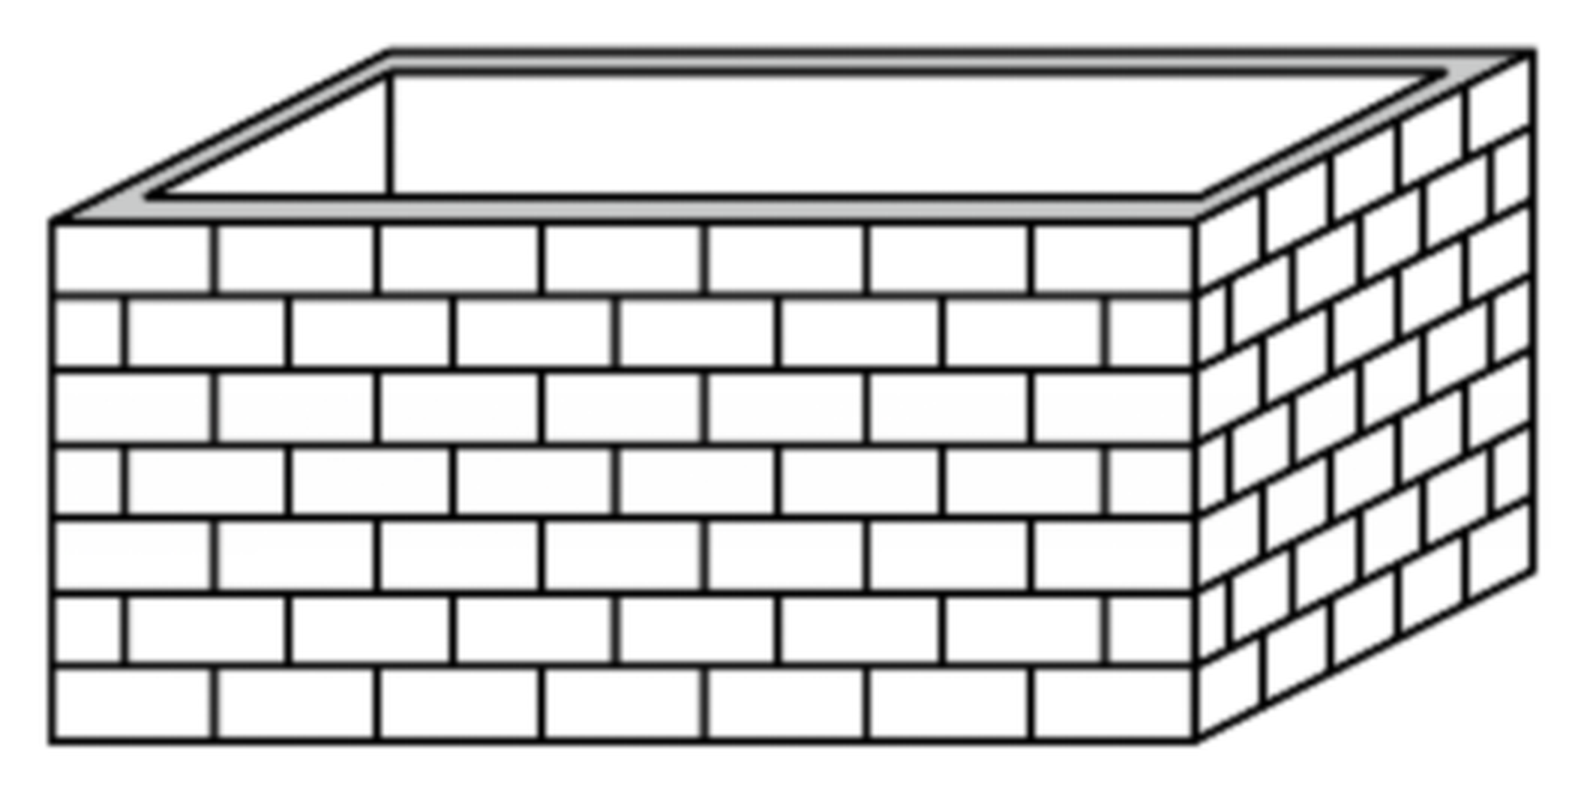
\includegraphics[width=0.42\textwidth]{figures/gao141_q19.png}
\end{center}

\ifanswer
\solbegin
\step{(1) 设水池的长、宽分别为 $xm$，$ym$，则 $x-y\geqslant60$，且 $x$、$y>0$，}
\step{由题意得 $2xy=3200$，即 $x=\dfrac{1600}{y}$，所以 $\dfrac{1600}{y}-y\geqslant60$，}
\step{因为 $y>0$，所以 $1600-y^2\geqslant60y$，}
\step{即 $y^2+60y-1600=(y+80)(y-20)\leqslant0$，解得 $-80\leqslant y\leqslant20$，}
\step{又 $y>0$，所以 $0<y\leqslant20$，所以水池的宽的最大值为 $20m$.}
\step{(2) 设水池总造价为 $z$ 元，}
\step{则 $z=1600\times150+2\times(2x+2y)\times120=240000+480(x+y)$，}
\step{又因为 $y=\dfrac{1600}{x}$，}
\step{所以 $z=240000+\left(x+\dfrac{1600}{x}\right)\times480\geqslant240000+480\times2\sqrt{1600}$}
\step{$=240000+38400=278400$，}
\step{当且仅当 $x=\dfrac{1600}{x}$，即 $x=y=40$ 时取等号，}
\step{所以，将水池的池底设计为边长为 $40m$ 的正方形时总造价最低，}
\step{最低总造价为 $278400$ 元.}
\solend
\fi

\item 已知 $a\in\R$，设集合 $A=\{x\mid ax^2-3x+2<ax-1\}$.

(1) 若 $A=(1,3)$，求实数 $a$ 的值；

(2) 当 $a>0$ 时，求 $A$；

(3) 若 “ $x\in\left(\dfrac12,+\infty\right)$ ” 是 “ $x\in A$ ” 的必要非充分条件，求实数 $a$ 的取值范围.

\ifanswer
\solbegin
\step{原不等式等价于 $ax^2-(a+3)x+3<0\Leftrightarrow(x-1)(ax-3)<0$，}
\step{(1) $A=(1,3)$ 为有界区间，因此 $a>0$，两根为 $1$ 和 $\dfrac3a$，于是 $\dfrac3a=3$，得 $a=1$；}
\step{此时 $(x-1)(x-3)<0$ 的解集确为 $(1,3)$.}
\step{(2) 当 $a>0$ 时，二次项系数为正，比较 $1$ 与 $\dfrac3a$，得 $A=\begin{cases}\left(1,\dfrac3a\right),&0<a<3\\\varnothing,&a=3\\\left(\dfrac3a,1\right),&a>3\end{cases}$，}
\step{其中 $a=3$ 时，原不等式为 $3(x-1)^2<0$，无解.}
\step{(3) 记 $S=\left(\dfrac12,+\infty\right)$，题意要求 $A\subset S$.}% 子集符号原卷印单线 $\subset$，照录
\step{由于对任意 $a$ 都有 $1\notin A$，而 $1\in S$，所以只需满足 $A\subseteq S$.}
\step{当 $a<0$ 时，$A=\left(-\infty,\dfrac3a\right)\cup(1,+\infty)$，含有小于 $\dfrac12$ 的数，不符合条件.}
\step{当 $a=0$ 时，$A=(1,+\infty)$，符合条件.}
\step{当 $0<a<3$ 时，$A=\left(1,\dfrac3a\right)\subseteq S$；}
\step{当 $a=3$ 时，$A=\varnothing\subseteq S$，均符合条件；}
\step{当 $a>3$ 时，$A=\left(\dfrac3a,1\right)$，所以 $A\subseteq S\Leftrightarrow\dfrac3a\geqslant\dfrac12\Leftrightarrow a\leqslant6$；}
\step{因此实数 $a$ 的取值范围为 $[0,6]$.}
\solend
\fi

\item 甲、乙两同学探讨了一个问题：已知正实数 $x,y$ 满足 $3x+y=1$，求 $\dfrac1x+\dfrac1y$ 的最小值.

甲给出的解法：由 $1=3x+y\geqslant2\sqrt{3xy}$，得 $\sqrt{xy}\leqslant\dfrac{\sqrt3}{6}$，所以 $\dfrac1x+\dfrac1y\geqslant2\sqrt{\dfrac1{xy}}\geqslant4\sqrt3$. 因此 $\dfrac1x+\dfrac1y$ 的最小值为 $4\sqrt3$.

乙给出的解法：$\dfrac1x+\dfrac1y=\left(\dfrac1x+\dfrac1y\right)(3x+y)=4+\dfrac yx+\dfrac{3x}{y}$，因为 $x,y$ 均为正实数，所以 $\dfrac1x+\dfrac1y\geqslant4+2\sqrt{\dfrac yx\cdot\dfrac{3x}{y}}=4+2\sqrt3$.

(1) 请判断上述哪位同学的解法正确，哪位同学的解法错误，并指出错误的原因；

(2) 结合上述探讨，试求当 $0<x<\dfrac12$ 时，$\dfrac1x+\dfrac1{1-2x}$ 的最小值以及此时实数 $x$ 的值；

(3) 已知 $x$ 为正实数，$y$ 为非负实数，且 $x+2y=2$，求 $\dfrac{x^2+1}{x}+\dfrac{2y^2}{y+1}$ 的最小值以及此时实数 $x,y$ 的值.

\ifanswer
\solbegin
\step{(1) 甲的推导中，$3x+y\geqslant2\sqrt{3xy}$ 取等号要求 $3x=y$，}
\step{$\dfrac1x+\dfrac1y\geqslant\dfrac2{\sqrt{xy}}$ 取等号要求 $x=y$，两者对正实数 $x,y$ 不能同时成立，}
\step{因此不能将 $4\sqrt3$ 判为最小值，甲错误.}
\step{乙的等号条件为 $\dfrac yx=\dfrac{3x}{y}$，即 $y=\sqrt3 x$；}
\step{结合 $3x+y=1$，得 $x=\dfrac1{3+\sqrt3},y=\dfrac{\sqrt3}{3+\sqrt3}$ 均为正数，等号可以成立，}
\step{因此乙正确，最小值为 $4+2\sqrt3$.}
\step{(2) 令 $t=1-2x>0$，则 $2x+t=1$.}
\step{$\dfrac1x+\dfrac1t=\left(\dfrac1x+\dfrac1t\right)(2x+t)=3+\dfrac tx+\dfrac{2x}{t}\geqslant3+2\sqrt2$，}
\step{当且仅当 $\dfrac tx=\dfrac{2x}{t}$，即 $t=\sqrt2 x$ 时取等号，}
\step{由 $2x+t=1$，得 $x=\dfrac1{2+\sqrt2}=\dfrac{2-\sqrt2}{2}\in\left(0,\dfrac12\right)$，}
\step{因此最小值为 $3+2\sqrt2$，此时 $x=\dfrac{2-\sqrt2}{2}$.}
\step{(3) 记目标式为 $F$，利用 $x+2y=2$，}
\step{得 $F=x+\dfrac1x+2y-2+\dfrac2{y+1}=\dfrac1x+\dfrac2{y+1}$，}
\step{又 $x+2(y+1)=4$，且 $x>0$、$y+1>0$，}
\step{所以 $4F=\left(\dfrac1x+\dfrac2{y+1}\right)(x+2(y+1))=5+2\left(\dfrac{y+1}{x}+\dfrac{x}{y+1}\right)$}
\step{$\geqslant5+2\times2=9$，当且仅当 $\dfrac{y+1}{x}=\dfrac{x}{y+1}$，即 $x=y+1$ 时取等号.}
\step{联立 $x+2y=2$，得 $x=\dfrac43$、$y=\dfrac13$，满足题设条件，}
\step{因此最小值为 $\dfrac94$，此时 $x=\dfrac43$，$y=\dfrac13$.}
\solend
\fi

\end{enumerate}

\end{document}
"
% 紧凑版：xelatex "\def\iscompact{1}% 高一141_彭浦中学_期中.tex
%   —— 高一上数学"2026-2027 年彭浦中学高一上期中"（试卷版/答案版/紧凑版）
% 试卷版：xelatex 高一141_彭浦中学_期中.tex
% 答案版：xelatex "\def\isanswer{1}% 高一141_彭浦中学_期中.tex
%   —— 高一上数学"2026-2027 年彭浦中学高一上期中"（试卷版/答案版/紧凑版）
% 试卷版：xelatex 高一141_彭浦中学_期中.tex
% 答案版：xelatex "\def\isanswer{1}\input{高一141_彭浦中学_期中.tex}"
% 紧凑版：xelatex "\def\iscompact{1}\input{高一141_彭浦中学_期中.tex}"
%
% ① 原始材料：微信公众号"魔都数学加油站"文章，连载"27学年高一141"，原文标题
% "27学年高一141——2026-2027年上海市彭浦中学高一上期中"；
% 原文链接：https://mp.weixin.qq.com/s/V_8bEhC6geeFyQysmtqUtQ。
% 正文为 9 张 PNG 页（01、05、06、07、09 为 2560x3620；02、03、04、08 为 4762x6735，
% 同一篇各页分辨率不同，逐页按各自分辨率放大裁图核对），题目下印【解析】，为讲评版。
% 题目、解析均据原图转录；卷面粉红色水印"魔都数学加油站"及公众号页脚未录入。
% 全卷 2 幅插图，均属题目配图（在 \ifanswer 外、三版都出）、取原卷截图去粉色水印、
% LANCZOS 放大 3 倍：第 5 题韦恩图（01 页，全集 U 矩形内两圆相交、交集阴影、A/B/U 标注）、
% 第 19 题长方体无盖贮水池砖墙示意图（06 页右上）。通读 9 页确认除这 2 幅外无其它
% 插图/表格，亦无"题干写如图而源码漏图"（仅 Q5"图中阴影部分"、Q19"如图所示"两处提到图）。
%
% 卷首标题：原卷印作"2026-2027 年彭浦中学高一上期中"（公众号标题中的"上海市"
% 卷面标题行没有，本稿照卷面），年份区间按全稿惯例排 en dash；原卷未印副标题，
% 本卷为期中卷、跨集合与常用逻辑用语／不等式／函数三章，按题目内容补出
% "集合与常用逻辑用语、不等式、函数"（与 高一140 同期中卷口径相同）：
% 集合与逻辑见 Q5、Q10、Q12、Q13、Q16、Q17、Q20，不等式见 Q4、Q9、Q14、Q18、
% Q19、Q21，函数（指数／对数）见 Q6、Q15。
%
% 题号体例：本卷共 19 题——一、填空题 3—12（10 题）、二、选择题 13—16（4 题）、
% 三、解答题 17—21（5 题）。三节分别 \setcounter{enumi}{2}／{12}／{16}。
% 原卷从第 3 题起、无第 1、2 题，本稿保留原题号；全卷无附加题节。
%
% ② 与原卷的排版差异：
%   ① 原文从第 3 题起，本稿保留原题号；
%   ② 原卷 19 题题下均印【解析】，无独立【答案】段、无"答案印题干括号且无解析"、
%      无"只印【答案】无解析"一型：填空题与解答题的答案落在【解析】末句
%      （Q3—Q12、Q17—Q21），四道选择题答案在【解析】末句"故选 …"
%      （Q13 选 A、Q14 选 C、Q15 选 D、Q16 选 C），题干括号内一律留空；
%      本稿 19 题一律 \solbegin…\solend、全卷不提 \ans{}，答案版【解析】标记数
%      = 19 = 全卷题数（无【答案】标记）；
%   ③ 原卷未印副标题，本稿按"知识模块"口径补出；
%   ④ 原卷填空横线按全稿惯例排 \blankline[4.4em]；选择题括号排 \mbox{（\quad）}，
%      选项段／命题段前按惯例加 \keepwithprev（Q16 两枚：命题列与选项段各一）；
%      解答题不留作答区、不加 \anspace（原卷为讲评版，与 129／131／132／133／136／140 同）；
%   ⑤ 原卷数集混排：黑板粗体 R（Q14 题干、Q16 ① 与解析、Q17 全集、Q20 题干）
%      按全稿惯例统一改 \R；空集记号 \varnothing；绝对值排 \lvert…\rvert，
%      集合描述竖线排 \mid；不等号按全稿惯例排 \leqslant／\geqslant；
%      补集照原卷上划线排 \overline{A\cap B}（Q17(2) 题干与解析）；
%      原卷"card"记号排黑体正体（Q12），本稿照录 \mathbf{card}，未改斜体
%      （与 高一66 同题口径不同：那份原卷 card 排斜体、照录 $card(M)$）；
%   ⑥ 子题标号 (1)(2)(3) 原卷印半角括号，照录；圈数字 ①②③④ 在正文（文本模式）
%      按原卷照录，未进数学式；数学式内半角逗号照录（如 Q12"$A,B$"、"{1,2,3}"、
%      Q14"$a,b,c\in\R$"、Q15"$\log_{14}7=a$，$14^b=5$"、Q16"$a=1,b=0$"、
%      Q18"$x,y,z$"、Q20"$x,y$"、Q21"$x,y$"）；全卷行末西文句点照录为 ASCII 句点；
%      行中全角逗号、顿号照录；
%   ⑦ 题干中的中文弯引号按原卷照录（Q13、Q20(3) 的 “ ” 及引号内空格），
%      注释内一律 ASCII 引号；
%   ⑧ 两幅题目配图各在 \item 之前加 \needvspace 守卫整块推走（Q5 5cm、Q19 6cm），
%      守卫放在 \item 之前而非 \bigsec 之后——两题均非各节首题，不触发 B 类
%      "节标题落页末"（照 高一26／40／59／136／140 成例）；三版切页审计均"合计异常：无"；
%   ⑨ 跨页续印按题合并：Q8 题干与【解析】首行在 01 页、后 6 行在 02 页；
%      Q15 题干在 03 页、【解析】在 04 页；Q17 题干与【解析】前 2 行在 04 页、
%      后 4 行在 05 页；Q19 题干在 05 页末、(1)(2) 小问与砖墙图与【解析】在 06 页；
%      Q20 题干 (1)(2) 在 06 页末、(3) 与【解析】在 07 页；Q21 题干与【解析】
%      前 6 行在 08 页、后 12 行在 09 页；Q16、Q18 全在各自页内；
%      本稿按题连排，不丢行；
%   ⑩ 原卷无红色加粗标签（【解析】均黑色印刷，Q16 解析 "①取…""④取…" 与
%      Q20 解析 "(2)" 等分步标签亦黑色），故本卷未用 \stepm；
%   ⑪ 原卷 Q19 题干把数值与单位（3200m³、2m、60m、150 元、120 元、40m、20m、
%      278400 元）印作略粗的西文字形，本稿按全稿惯例（高一70／72 同类题）排普通
%      数学体，未加粗。
%
% ③ 行数复核：一条 \step = 原卷解析的一个印刷行，cases 块作一个印刷行计。逐题数 \step
%   条数，合计 92 条（Q3：1；Q4：1；Q5：1；Q6：1；Q7：2；Q8：7；Q9：1；Q10：4；
%   Q11：4；Q12：4；Q13：2；Q14：1；Q15：2；Q16：4；Q17：6；Q18：7；Q19：13；
%   Q20：13；Q21：18），与原卷印刷行逐题相等。全卷 19 题均印【解析】、无独立 \ans{}，
%   答案版【解析】标记数 = 19 = 全卷题数。
%
% ④ 判别式／子集符号结论（逐处放大原图照录、不得统一）：
%   判别式：全卷 3 处——第 7 题【解析】"$\Delta=a^2-4\cdot\frac14=0$"一处原卷印
%     等腰、偏高的高三角 $\Delta$，照录 \Delta；第 8 题【解析】
%     "$\triangle=25-40=-15<0$"与"$\triangle=1+8=9>0$"两处原卷印扁等边三角
%     $\triangle$，照录 \triangle。两形不同，逐处照录未统一。
%   子集：全卷 6 处——第 10 题【解析】"$B\subseteq A$"一处、第 20 题【解析】
%     "所以只需满足 $A\subseteq S$"、"$A=\left(1,\frac3a\right)\subseteq S$"、
%     "$A=\varnothing\subseteq S$"、"$A\subseteq S\Leftrightarrow\frac3a\geqslant\frac12$"
%     四处，共 5 处原卷印带下划线的 $\subseteq$，照录 \subseteq；第 20 题【解析】
%     (3) 首行"题意要求 $A\subset S$"一处原卷印单线 $\subset$，照录 \subset
%     （下行因 $1\in S$ 而 $1\notin A$，改述为 $A\subseteq S$，两者逻辑一致、非笔误）。
%
% ⑤ 存疑照录（照录未改，正文对应处另有 % 注）：
%   第 14 题题干"设 $a,b,c\in\R$"只声明 $a,b,c$，而 A 选项"若 $a>b$ 且 $c>d$，
%     则 $ac>bd$"引入未声明的 $d$，原卷变量声明与选项不统一，照录未补。
%   全卷除此 1 条外未发现其它笔误／自相矛盾处。
%
% ⑥ 跨页续印按题合并说明：见 ② ⑨。
%
\documentclass[a4paper,11pt]{article}
\usepackage{common}

\begin{document}

\examtitlest[3]{2026--2027 年彭浦中学高一上期中}{集合与常用逻辑用语、不等式、函数}

\bigsec{一、填空题}

\begin{enumerate}
\setcounter{enumi}{2}

\item 已知 $m$ 为实数，若 $1\in\{m,m^2\}$，则 $m$ 的值为\blankline[4.4em].

\ifanswer
\solbegin
\step{$m=1$ 或 $m^2=1$，得 $m=\pm1$；按列举项互异口径排除 $m=m^2=1$，得 $m=-1$.}
\solend
\fi

\item 已知 $2<a<4$，$-2<b<1$，则 $2a+b$ 的取值范围为\blankline[4.4em].

\ifanswer
\solbegin
\step{$4<2a<8$，与 $-2<b<1$ 相加，得 $2<2a+b<9$，取值范围为 $(2,9)$.}
\solend
\fi

% 第 5 题韦恩图（题目配图，三版都出）：取原卷 01 页截图去粉色水印、LANCZOS 放大 3 倍
\needvspace{5cm}
\item 已知集合 $A=\{-1,-2,1,4,7\}$，$B=\{x\mid x>1\}$，用列举法表示图中阴影部分所表示的集合为\blankline[4.4em].

\begin{center}
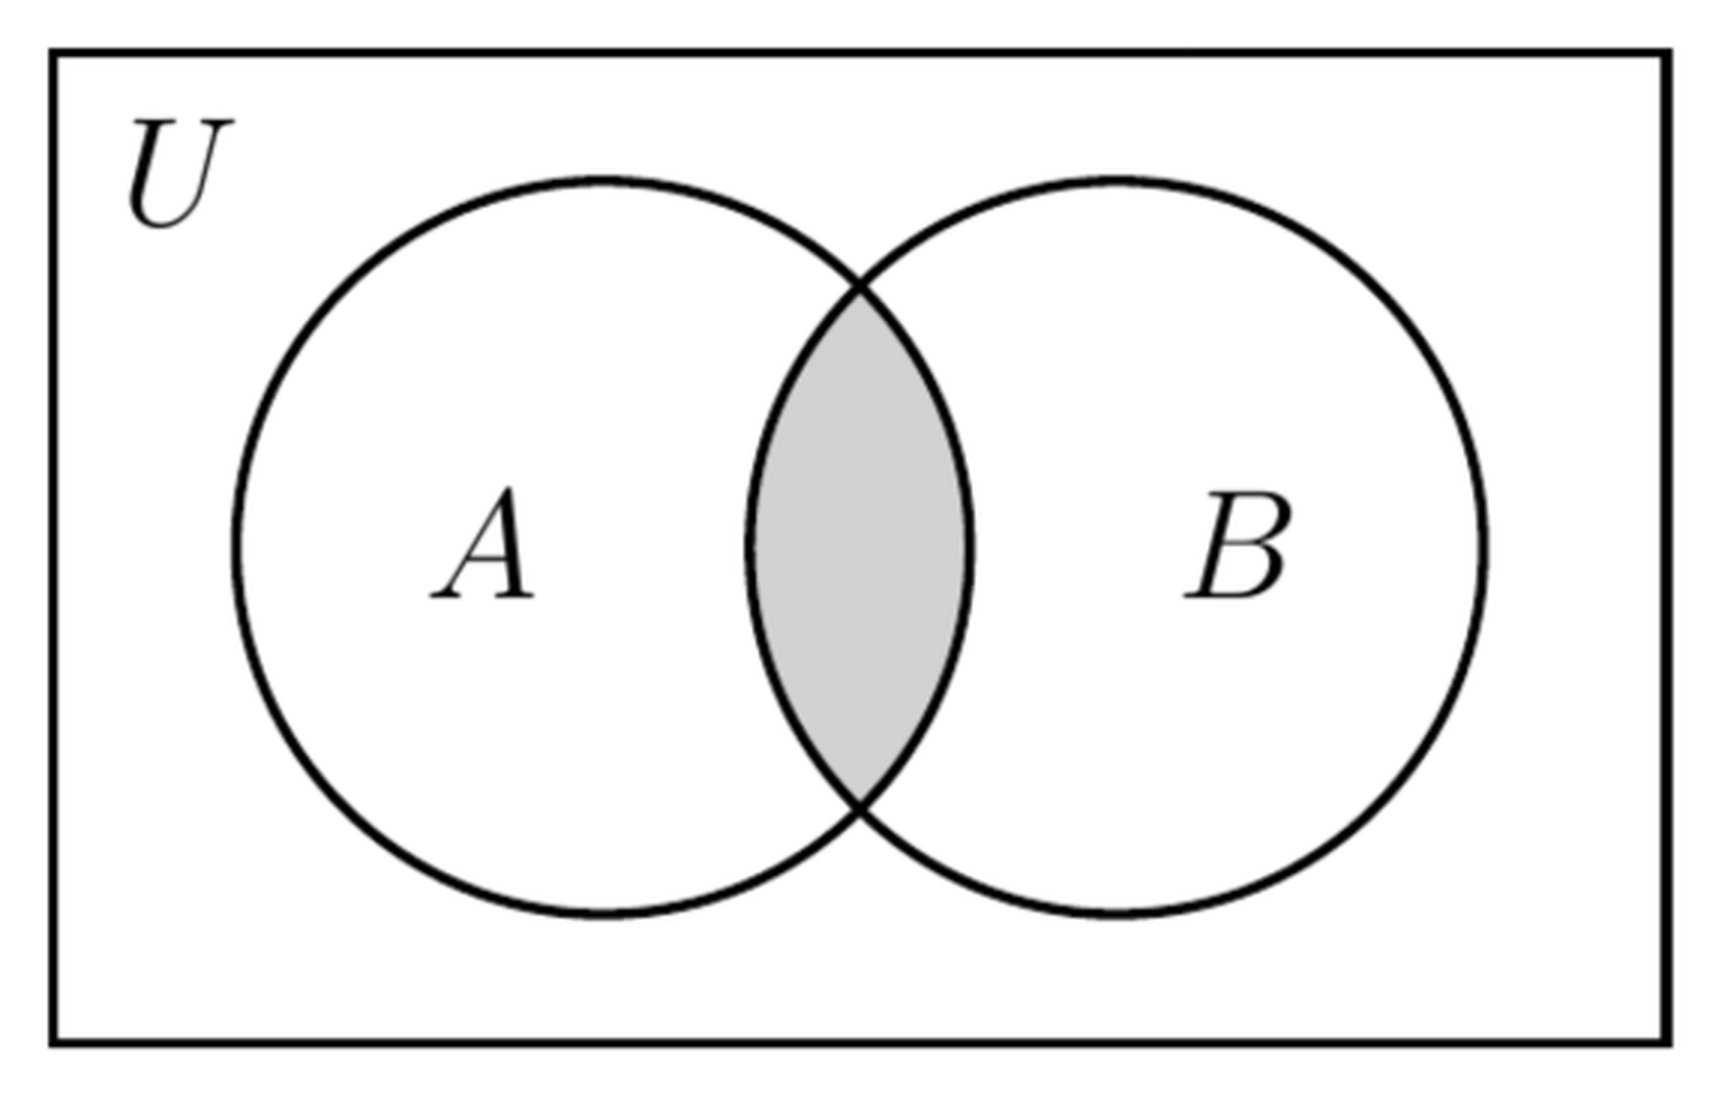
\includegraphics[width=0.38\textwidth]{figures/gao141_q5.png}
\end{center}

\ifanswer
\solbegin
\step{阴影部分表示 $A\cap B=\{4,7\}$.}
\solend
\fi

\item 方程 $2^{\log_3 x}=\dfrac12$ 的解集为\blankline[4.4em].

\ifanswer
\solbegin
\step{$2^{\log_3 x}=2^{-1}\Leftrightarrow\log_3 x=-1\Leftrightarrow x=\dfrac13$，解集为 $\left\{\dfrac13\right\}$.}
\solend
\fi

\item 若集合 $A=\left\{x\mid x^2+ax+\dfrac14=0\right\}$ 有且仅有两个子集，则实数 $a$ 的值为\blankline[4.4em].

\ifanswer
\solbegin
\step{$A$ 有且仅有两个子集，说明 $A$ 恰有一个元素，即方程有两个相等的实数根.}
\step{$\Delta=a^2-4\cdot\dfrac14=0\Rightarrow a=\pm1$.}% 判别式原卷印等腰偏高的高三角 $\Delta$，照录
\solend
\fi

\item 已知关于 $x$ 的方程 $x^2+mx+2m=0$ 的两个实数根分别为 $\alpha$、$\beta$，若 $\alpha^2+\beta^2=5$，则实数 $m=$\blankline[4.4em].

\ifanswer
\solbegin
\step{方程 $x^2+mx+2m=0$ 的两个实数根为 $\alpha$、$\beta$，}
\step{由根与系数的关系得 $\begin{cases}\alpha+\beta=-m\\\alpha\beta=2m\end{cases}$，又因为 $\alpha^2+\beta^2=5$，}
\step{所以 $\alpha^2+\beta^2=(\alpha+\beta)^2-2\alpha\beta=m^2-4m=5$，整理得 $m^2-4m-5=0$，}
\step{解得 $m=5$ 或 $m=-1$，}
\step{当 $m=5$ 时，$\triangle=25-40=-15<0$，无实根，舍去；}% 判别式原卷印扁等边三角 $\triangle$，照录
\step{当 $m=-1$ 时，$\triangle=1+8=9>0$，符合题意，}
\step{所以实数 $m=-1$.}
\solend
\fi

\item 若不等式 $\lvert x-3\rvert+\lvert x-5\rvert\geqslant a$ 对任意的实数 $x$ 恒成立，则实数 $a$ 的取值范围为\blankline[4.4em].

\ifanswer
\solbegin
\step{由三角不等式得 $\lvert x-3\rvert+\lvert x-5\rvert\geqslant\lvert x-3-x+5\rvert=2$，则 $a\leqslant2$.}
\solend
\fi

\item 设集合 $A=\{-3,2\}$，集合 $B=\{x\mid mx+1=0\}$，若 $A\cup B=A$，则实数 $m$ 的值为\blankline[4.4em].

\ifanswer
\solbegin
\step{由 $A\cup B=A$，得 $B\subseteq A$，}% 子集符号原卷印带下划线的 $\subseteq$，照录
\step{当 $m=0$ 时，$B=\varnothing$，满足题意，}
\step{当 $m\neq0$ 时，$B=\left\{-\dfrac1m\right\}$，所以 $-\dfrac1m=2$ 或 $-\dfrac1m=-3$，所以 $m=-\dfrac12$ 或 $m=\dfrac13$，}
\step{综上所述，$m=0$ 或 $m=-\dfrac12$ 或 $m=\dfrac13$.}
\solend
\fi

\item 已知 $m$ 为实数，代数式 $M=\sqrt{m-1}+\sqrt{3-m}$ 的取值范围为\blankline[4.4em].

\ifanswer
\solbegin
\step{根式有意义要求 $m\in[1,3]$，}
\step{此时 $(m-1)(3-m)=1-(m-2)^2$ 的取值范围为 $[0,1]$.}
\step{$M^2=2+2\sqrt{(m-1)(3-m)}$ 的取值范围为 $[2,4]$，又 $M>0$，}
\step{所以 $M\in[\sqrt2,2]$.}
\solend
\fi

\item 设有限集 $M$ 所含元素的个数用 $\mathbf{card}(M)$ 表示，并规定 $\mathbf{card}(\varnothing)=0$. 已知集合 $A,B$ 满足 $A\cup B=\{1,2,3\}$，$A\cap B=\varnothing$，若 $\mathbf{card}(A)\notin A$，$\mathbf{card}(B)\notin B$，则满足条件的所有不同集合 $A$ 的个数为\blankline[4.4em].

\ifanswer
\solbegin
\step{当 $\mathbf{card}(A)=0$ 或 $3$ 时，$A,B$ 中有一个为 $\{1,2,3\}$，不符合条件.}
\step{当 $\mathbf{card}(A)=1$ 时，$\mathbf{card}(B)=2\notin B$，所以 $A=\{2\}$，符合条件.}
\step{当 $\mathbf{card}(A)=2$ 时，$2\notin A$，所以 $B=\{2\}$，$A=\{1,3\}$，符合条件.}
\step{满足条件的集合 $A$ 共 $2$ 个.}
\solend
\fi

\end{enumerate}

\bigsec{二、选择题}

\begin{enumerate}
\setcounter{enumi}{12}

\item “ $x=1$ ” 是 “ $x^2-3x+2=0$ ” 的\mbox{（\quad）}条件.

\keepwithprev
A. 充分非必要\qquad B. 必要非充分

C. 充要\qquad D. 既非充分又非必要

\ifanswer
\solbegin
\step{$x^2-3x+2=0\Leftrightarrow x=1$ 或 $x=2$，所以 “ $x=1$ ” 是其充分非必要条件，}
\step{故选 $A$.}
\solend
\fi

\item 设 $a,b,c\in\R$，则下列命题为真命题的是\mbox{（\quad）}
% 原卷题干只声明 a,b,c，而 A 选项出现未声明的 d，照录（存疑）
\keepwithprev
A. 若 $a>b$ 且 $c>d$，则 $ac>bd$\qquad B. 若 $a^2>b^2$，则 $a>b$

C. 若 $ab>0$ 且 $a>b$，则 $\dfrac1a<\dfrac1b$\qquad D. 若 $a<0<b$，则 $\sqrt{-a}<\sqrt b$

\ifanswer
\solbegin
\step{$ab>0$ 且 $a>b\Rightarrow\dfrac1a-\dfrac1b=\dfrac{b-a}{ab}<0$，所以 $C$ 为真命题，故选 $C$.}
\solend
\fi

\item 已知 $\log_{14}7=a$，$14^b=5$，则 $\log_{35}28=$\mbox{（\quad）}

\keepwithprev
A. $\dfrac{2-a}{2a+b}$\qquad B. $\dfrac{2+a}{a+b}$\qquad C. $\dfrac{2-a}{a+2b}$\qquad D. $\dfrac{2-a}{a+b}$

\ifanswer
\solbegin
\step{$\log_{14}7=a$，$14^b=5$，}
\step{$\log_{35}28=\dfrac{\log_{14}28}{\log_{14}35}=\dfrac{\log_{14}14^2-\log_{14}7}{\log_{14}7+\log_{14}5}=\dfrac{2-a}{a+b}$. 故选 $D$.}
\solend
\fi

\item 关于 $x$ 的不等式 $ax^2+bx+3>0$ 的解集有下列说法，其中正确的个数是\mbox{（\quad）}

\keepwithprev
① 不等式 $ax^2+bx+3>0$ 的解集可以是 $\R$

② 不等式 $ax^2+bx+3>0$ 的解集可以是 $\{x\mid x>3\}$

③ 不等式 $ax^2+bx+3>0$ 的解集可以是 $\varnothing$

④ 不等式 $ax^2+bx+3>0$ 的解集可以是 $\{x\mid -1<x<3\}$

\keepwithprev
A. 4\qquad B. 3\qquad C. 2\qquad D. 1

\ifanswer
\solbegin
\step{$x=0$ 时左端为 $3>0$，解集必含 $0$，所以②③错误.}
\step{①取 $a=1,b=0$，$x^2+3>0$ 的解集为 $\R$，正确.}
\step{④取 $a=-1,b=2$，$-x^2+2x+3=-(x+1)(x-3)>0\Leftrightarrow-1<x<3$，正确.}
\step{正确的有①④，共 $2$ 个，故选 $C$.}
\solend
\fi

\end{enumerate}

\bigsec{三、解答题}

\begin{enumerate}
\setcounter{enumi}{16}

\item 已知集合 $A=\left\{x\mid\dfrac{x-2}{x+3}\geqslant0\right\}$，集合 $B=\{x\mid\lvert x+1\rvert+\lvert x-1\rvert<5\}$，全集 $U=\R$.

(1) 求 $A,B$；

(2) 求 $A\cup B$、$\overline{A\cap B}$.

\ifanswer
\solbegin
\step{(1) 分母不为零，且分子、分母同号或分子为零，}
\step{所以 $\dfrac{x-2}{x+3}\geqslant0\Leftrightarrow x<-3$ 或 $x\geqslant2$，因此 $A=(-\infty,-3)\cup[2,+\infty)$.}
\step{又 $\lvert x+1\rvert+\lvert x-1\rvert=\begin{cases}-2x,&x<-1\\2,&-1\leqslant x\leqslant1\\2x,&x>1\end{cases}$，}
\step{分别解得 $-\dfrac52<x<-1$、$-1\leqslant x\leqslant1$、$1<x<\dfrac52$，因此 $B=\left(-\dfrac52,\dfrac52\right)$.}
\step{(2) 合并两集合所对应的区间，得 $A\cup B=(-\infty,-3)\cup\left(-\dfrac52,+\infty\right)$，}
\step{两集合的公共部分为 $A\cap B=\left[2,\dfrac52\right)$，所以 $\overline{A\cap B}=(-\infty,2)\cup\left[\dfrac52,+\infty\right)$.}
\solend
\fi

\item (1) 已知 $a>b>0$，比较代数式 $\dfrac ab$ 与 $\dfrac{a+1}{b+1}$ 的大小并说明理由；

(2) 已知 $x,y,z$ 都是正实数，$a=x+\dfrac1y,b=y+\dfrac1z,c=z+\dfrac1x$，试用反证法证明 $a,b,c$ 至少有一个不小于 $2$.

\ifanswer
\solbegin
\step{(1) $\dfrac ab-\dfrac{a+1}{b+1}=\dfrac{a(b+1)-b(a+1)}{b(b+1)}=\dfrac{a-b}{b(b+1)}$，}
\step{因为 $a>b>0$，所以 $a-b>0$，$b(b+1)>0$，所以 $\dfrac ab-\dfrac{a+1}{b+1}>0$，}
\step{故 $\dfrac ab>\dfrac{a+1}{b+1}$.}
\step{(2) 假设 $a$、$b$、$c$ 三数都小于 $2$，则 $x+\dfrac1y+y+\dfrac1z+z+\dfrac1x<6$.}
\step{因为 $x,y,z$ 均大于 $0$，}
\step{所以 $x+\dfrac1y+y+\dfrac1z+z+\dfrac1x=x+\dfrac1x+y+\dfrac1y+z+\dfrac1z\geqslant2+2+2=6$，矛盾，}
\step{所以 $a$、$b$、$c$ 三数中至少有一个不小于 $2$.}
\solend
\fi

% 第 19 题长方体无盖贮水池砖墙示意图（题目配图，三版都出）：取原卷 06 页截图去粉色水印、LANCZOS 放大 3 倍
\needvspace{6cm}
\item 如图所示，某工厂要建造一个长方体形无盖贮水池，其容积为 $3200m^3$，深为 $2m$.

(1) 若水池的长比宽至少多 $60m$，求水池的宽的最大值；

(2) 若池底每平方米的造价为 $150$ 元，池壁每平方米的造价为 $120$ 元，那么怎样设计水池的长和宽能使总造价最低？最低总造价是多少？

\begin{center}
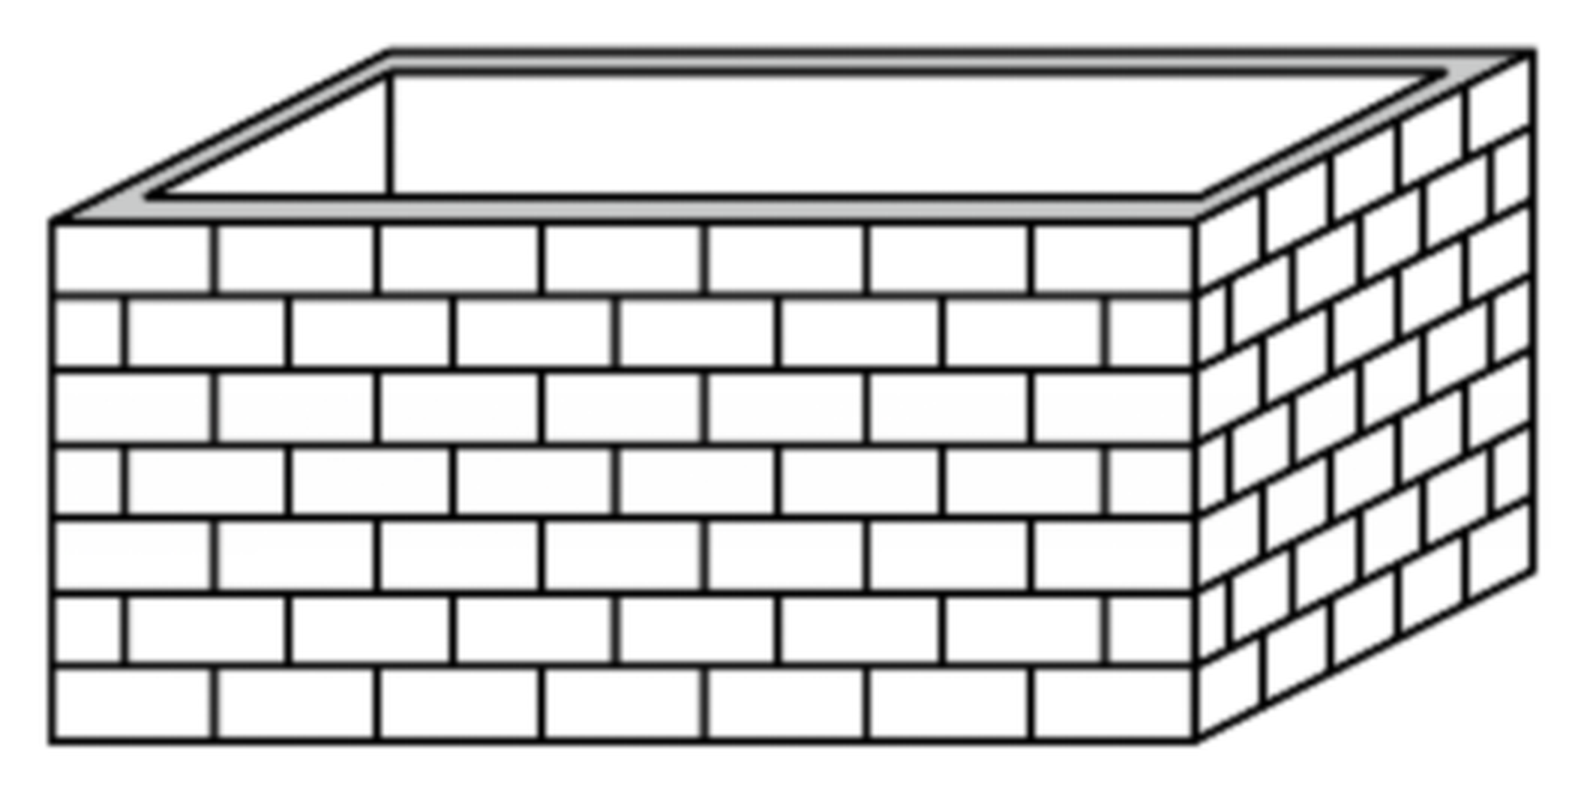
\includegraphics[width=0.42\textwidth]{figures/gao141_q19.png}
\end{center}

\ifanswer
\solbegin
\step{(1) 设水池的长、宽分别为 $xm$，$ym$，则 $x-y\geqslant60$，且 $x$、$y>0$，}
\step{由题意得 $2xy=3200$，即 $x=\dfrac{1600}{y}$，所以 $\dfrac{1600}{y}-y\geqslant60$，}
\step{因为 $y>0$，所以 $1600-y^2\geqslant60y$，}
\step{即 $y^2+60y-1600=(y+80)(y-20)\leqslant0$，解得 $-80\leqslant y\leqslant20$，}
\step{又 $y>0$，所以 $0<y\leqslant20$，所以水池的宽的最大值为 $20m$.}
\step{(2) 设水池总造价为 $z$ 元，}
\step{则 $z=1600\times150+2\times(2x+2y)\times120=240000+480(x+y)$，}
\step{又因为 $y=\dfrac{1600}{x}$，}
\step{所以 $z=240000+\left(x+\dfrac{1600}{x}\right)\times480\geqslant240000+480\times2\sqrt{1600}$}
\step{$=240000+38400=278400$，}
\step{当且仅当 $x=\dfrac{1600}{x}$，即 $x=y=40$ 时取等号，}
\step{所以，将水池的池底设计为边长为 $40m$ 的正方形时总造价最低，}
\step{最低总造价为 $278400$ 元.}
\solend
\fi

\item 已知 $a\in\R$，设集合 $A=\{x\mid ax^2-3x+2<ax-1\}$.

(1) 若 $A=(1,3)$，求实数 $a$ 的值；

(2) 当 $a>0$ 时，求 $A$；

(3) 若 “ $x\in\left(\dfrac12,+\infty\right)$ ” 是 “ $x\in A$ ” 的必要非充分条件，求实数 $a$ 的取值范围.

\ifanswer
\solbegin
\step{原不等式等价于 $ax^2-(a+3)x+3<0\Leftrightarrow(x-1)(ax-3)<0$，}
\step{(1) $A=(1,3)$ 为有界区间，因此 $a>0$，两根为 $1$ 和 $\dfrac3a$，于是 $\dfrac3a=3$，得 $a=1$；}
\step{此时 $(x-1)(x-3)<0$ 的解集确为 $(1,3)$.}
\step{(2) 当 $a>0$ 时，二次项系数为正，比较 $1$ 与 $\dfrac3a$，得 $A=\begin{cases}\left(1,\dfrac3a\right),&0<a<3\\\varnothing,&a=3\\\left(\dfrac3a,1\right),&a>3\end{cases}$，}
\step{其中 $a=3$ 时，原不等式为 $3(x-1)^2<0$，无解.}
\step{(3) 记 $S=\left(\dfrac12,+\infty\right)$，题意要求 $A\subset S$.}% 子集符号原卷印单线 $\subset$，照录
\step{由于对任意 $a$ 都有 $1\notin A$，而 $1\in S$，所以只需满足 $A\subseteq S$.}
\step{当 $a<0$ 时，$A=\left(-\infty,\dfrac3a\right)\cup(1,+\infty)$，含有小于 $\dfrac12$ 的数，不符合条件.}
\step{当 $a=0$ 时，$A=(1,+\infty)$，符合条件.}
\step{当 $0<a<3$ 时，$A=\left(1,\dfrac3a\right)\subseteq S$；}
\step{当 $a=3$ 时，$A=\varnothing\subseteq S$，均符合条件；}
\step{当 $a>3$ 时，$A=\left(\dfrac3a,1\right)$，所以 $A\subseteq S\Leftrightarrow\dfrac3a\geqslant\dfrac12\Leftrightarrow a\leqslant6$；}
\step{因此实数 $a$ 的取值范围为 $[0,6]$.}
\solend
\fi

\item 甲、乙两同学探讨了一个问题：已知正实数 $x,y$ 满足 $3x+y=1$，求 $\dfrac1x+\dfrac1y$ 的最小值.

甲给出的解法：由 $1=3x+y\geqslant2\sqrt{3xy}$，得 $\sqrt{xy}\leqslant\dfrac{\sqrt3}{6}$，所以 $\dfrac1x+\dfrac1y\geqslant2\sqrt{\dfrac1{xy}}\geqslant4\sqrt3$. 因此 $\dfrac1x+\dfrac1y$ 的最小值为 $4\sqrt3$.

乙给出的解法：$\dfrac1x+\dfrac1y=\left(\dfrac1x+\dfrac1y\right)(3x+y)=4+\dfrac yx+\dfrac{3x}{y}$，因为 $x,y$ 均为正实数，所以 $\dfrac1x+\dfrac1y\geqslant4+2\sqrt{\dfrac yx\cdot\dfrac{3x}{y}}=4+2\sqrt3$.

(1) 请判断上述哪位同学的解法正确，哪位同学的解法错误，并指出错误的原因；

(2) 结合上述探讨，试求当 $0<x<\dfrac12$ 时，$\dfrac1x+\dfrac1{1-2x}$ 的最小值以及此时实数 $x$ 的值；

(3) 已知 $x$ 为正实数，$y$ 为非负实数，且 $x+2y=2$，求 $\dfrac{x^2+1}{x}+\dfrac{2y^2}{y+1}$ 的最小值以及此时实数 $x,y$ 的值.

\ifanswer
\solbegin
\step{(1) 甲的推导中，$3x+y\geqslant2\sqrt{3xy}$ 取等号要求 $3x=y$，}
\step{$\dfrac1x+\dfrac1y\geqslant\dfrac2{\sqrt{xy}}$ 取等号要求 $x=y$，两者对正实数 $x,y$ 不能同时成立，}
\step{因此不能将 $4\sqrt3$ 判为最小值，甲错误.}
\step{乙的等号条件为 $\dfrac yx=\dfrac{3x}{y}$，即 $y=\sqrt3 x$；}
\step{结合 $3x+y=1$，得 $x=\dfrac1{3+\sqrt3},y=\dfrac{\sqrt3}{3+\sqrt3}$ 均为正数，等号可以成立，}
\step{因此乙正确，最小值为 $4+2\sqrt3$.}
\step{(2) 令 $t=1-2x>0$，则 $2x+t=1$.}
\step{$\dfrac1x+\dfrac1t=\left(\dfrac1x+\dfrac1t\right)(2x+t)=3+\dfrac tx+\dfrac{2x}{t}\geqslant3+2\sqrt2$，}
\step{当且仅当 $\dfrac tx=\dfrac{2x}{t}$，即 $t=\sqrt2 x$ 时取等号，}
\step{由 $2x+t=1$，得 $x=\dfrac1{2+\sqrt2}=\dfrac{2-\sqrt2}{2}\in\left(0,\dfrac12\right)$，}
\step{因此最小值为 $3+2\sqrt2$，此时 $x=\dfrac{2-\sqrt2}{2}$.}
\step{(3) 记目标式为 $F$，利用 $x+2y=2$，}
\step{得 $F=x+\dfrac1x+2y-2+\dfrac2{y+1}=\dfrac1x+\dfrac2{y+1}$，}
\step{又 $x+2(y+1)=4$，且 $x>0$、$y+1>0$，}
\step{所以 $4F=\left(\dfrac1x+\dfrac2{y+1}\right)(x+2(y+1))=5+2\left(\dfrac{y+1}{x}+\dfrac{x}{y+1}\right)$}
\step{$\geqslant5+2\times2=9$，当且仅当 $\dfrac{y+1}{x}=\dfrac{x}{y+1}$，即 $x=y+1$ 时取等号.}
\step{联立 $x+2y=2$，得 $x=\dfrac43$、$y=\dfrac13$，满足题设条件，}
\step{因此最小值为 $\dfrac94$，此时 $x=\dfrac43$，$y=\dfrac13$.}
\solend
\fi

\end{enumerate}

\end{document}
"
% 紧凑版：xelatex "\def\iscompact{1}% 高一141_彭浦中学_期中.tex
%   —— 高一上数学"2026-2027 年彭浦中学高一上期中"（试卷版/答案版/紧凑版）
% 试卷版：xelatex 高一141_彭浦中学_期中.tex
% 答案版：xelatex "\def\isanswer{1}\input{高一141_彭浦中学_期中.tex}"
% 紧凑版：xelatex "\def\iscompact{1}\input{高一141_彭浦中学_期中.tex}"
%
% ① 原始材料：微信公众号"魔都数学加油站"文章，连载"27学年高一141"，原文标题
% "27学年高一141——2026-2027年上海市彭浦中学高一上期中"；
% 原文链接：https://mp.weixin.qq.com/s/V_8bEhC6geeFyQysmtqUtQ。
% 正文为 9 张 PNG 页（01、05、06、07、09 为 2560x3620；02、03、04、08 为 4762x6735，
% 同一篇各页分辨率不同，逐页按各自分辨率放大裁图核对），题目下印【解析】，为讲评版。
% 题目、解析均据原图转录；卷面粉红色水印"魔都数学加油站"及公众号页脚未录入。
% 全卷 2 幅插图，均属题目配图（在 \ifanswer 外、三版都出）、取原卷截图去粉色水印、
% LANCZOS 放大 3 倍：第 5 题韦恩图（01 页，全集 U 矩形内两圆相交、交集阴影、A/B/U 标注）、
% 第 19 题长方体无盖贮水池砖墙示意图（06 页右上）。通读 9 页确认除这 2 幅外无其它
% 插图/表格，亦无"题干写如图而源码漏图"（仅 Q5"图中阴影部分"、Q19"如图所示"两处提到图）。
%
% 卷首标题：原卷印作"2026-2027 年彭浦中学高一上期中"（公众号标题中的"上海市"
% 卷面标题行没有，本稿照卷面），年份区间按全稿惯例排 en dash；原卷未印副标题，
% 本卷为期中卷、跨集合与常用逻辑用语／不等式／函数三章，按题目内容补出
% "集合与常用逻辑用语、不等式、函数"（与 高一140 同期中卷口径相同）：
% 集合与逻辑见 Q5、Q10、Q12、Q13、Q16、Q17、Q20，不等式见 Q4、Q9、Q14、Q18、
% Q19、Q21，函数（指数／对数）见 Q6、Q15。
%
% 题号体例：本卷共 19 题——一、填空题 3—12（10 题）、二、选择题 13—16（4 题）、
% 三、解答题 17—21（5 题）。三节分别 \setcounter{enumi}{2}／{12}／{16}。
% 原卷从第 3 题起、无第 1、2 题，本稿保留原题号；全卷无附加题节。
%
% ② 与原卷的排版差异：
%   ① 原文从第 3 题起，本稿保留原题号；
%   ② 原卷 19 题题下均印【解析】，无独立【答案】段、无"答案印题干括号且无解析"、
%      无"只印【答案】无解析"一型：填空题与解答题的答案落在【解析】末句
%      （Q3—Q12、Q17—Q21），四道选择题答案在【解析】末句"故选 …"
%      （Q13 选 A、Q14 选 C、Q15 选 D、Q16 选 C），题干括号内一律留空；
%      本稿 19 题一律 \solbegin…\solend、全卷不提 \ans{}，答案版【解析】标记数
%      = 19 = 全卷题数（无【答案】标记）；
%   ③ 原卷未印副标题，本稿按"知识模块"口径补出；
%   ④ 原卷填空横线按全稿惯例排 \blankline[4.4em]；选择题括号排 \mbox{（\quad）}，
%      选项段／命题段前按惯例加 \keepwithprev（Q16 两枚：命题列与选项段各一）；
%      解答题不留作答区、不加 \anspace（原卷为讲评版，与 129／131／132／133／136／140 同）；
%   ⑤ 原卷数集混排：黑板粗体 R（Q14 题干、Q16 ① 与解析、Q17 全集、Q20 题干）
%      按全稿惯例统一改 \R；空集记号 \varnothing；绝对值排 \lvert…\rvert，
%      集合描述竖线排 \mid；不等号按全稿惯例排 \leqslant／\geqslant；
%      补集照原卷上划线排 \overline{A\cap B}（Q17(2) 题干与解析）；
%      原卷"card"记号排黑体正体（Q12），本稿照录 \mathbf{card}，未改斜体
%      （与 高一66 同题口径不同：那份原卷 card 排斜体、照录 $card(M)$）；
%   ⑥ 子题标号 (1)(2)(3) 原卷印半角括号，照录；圈数字 ①②③④ 在正文（文本模式）
%      按原卷照录，未进数学式；数学式内半角逗号照录（如 Q12"$A,B$"、"{1,2,3}"、
%      Q14"$a,b,c\in\R$"、Q15"$\log_{14}7=a$，$14^b=5$"、Q16"$a=1,b=0$"、
%      Q18"$x,y,z$"、Q20"$x,y$"、Q21"$x,y$"）；全卷行末西文句点照录为 ASCII 句点；
%      行中全角逗号、顿号照录；
%   ⑦ 题干中的中文弯引号按原卷照录（Q13、Q20(3) 的 “ ” 及引号内空格），
%      注释内一律 ASCII 引号；
%   ⑧ 两幅题目配图各在 \item 之前加 \needvspace 守卫整块推走（Q5 5cm、Q19 6cm），
%      守卫放在 \item 之前而非 \bigsec 之后——两题均非各节首题，不触发 B 类
%      "节标题落页末"（照 高一26／40／59／136／140 成例）；三版切页审计均"合计异常：无"；
%   ⑨ 跨页续印按题合并：Q8 题干与【解析】首行在 01 页、后 6 行在 02 页；
%      Q15 题干在 03 页、【解析】在 04 页；Q17 题干与【解析】前 2 行在 04 页、
%      后 4 行在 05 页；Q19 题干在 05 页末、(1)(2) 小问与砖墙图与【解析】在 06 页；
%      Q20 题干 (1)(2) 在 06 页末、(3) 与【解析】在 07 页；Q21 题干与【解析】
%      前 6 行在 08 页、后 12 行在 09 页；Q16、Q18 全在各自页内；
%      本稿按题连排，不丢行；
%   ⑩ 原卷无红色加粗标签（【解析】均黑色印刷，Q16 解析 "①取…""④取…" 与
%      Q20 解析 "(2)" 等分步标签亦黑色），故本卷未用 \stepm；
%   ⑪ 原卷 Q19 题干把数值与单位（3200m³、2m、60m、150 元、120 元、40m、20m、
%      278400 元）印作略粗的西文字形，本稿按全稿惯例（高一70／72 同类题）排普通
%      数学体，未加粗。
%
% ③ 行数复核：一条 \step = 原卷解析的一个印刷行，cases 块作一个印刷行计。逐题数 \step
%   条数，合计 92 条（Q3：1；Q4：1；Q5：1；Q6：1；Q7：2；Q8：7；Q9：1；Q10：4；
%   Q11：4；Q12：4；Q13：2；Q14：1；Q15：2；Q16：4；Q17：6；Q18：7；Q19：13；
%   Q20：13；Q21：18），与原卷印刷行逐题相等。全卷 19 题均印【解析】、无独立 \ans{}，
%   答案版【解析】标记数 = 19 = 全卷题数。
%
% ④ 判别式／子集符号结论（逐处放大原图照录、不得统一）：
%   判别式：全卷 3 处——第 7 题【解析】"$\Delta=a^2-4\cdot\frac14=0$"一处原卷印
%     等腰、偏高的高三角 $\Delta$，照录 \Delta；第 8 题【解析】
%     "$\triangle=25-40=-15<0$"与"$\triangle=1+8=9>0$"两处原卷印扁等边三角
%     $\triangle$，照录 \triangle。两形不同，逐处照录未统一。
%   子集：全卷 6 处——第 10 题【解析】"$B\subseteq A$"一处、第 20 题【解析】
%     "所以只需满足 $A\subseteq S$"、"$A=\left(1,\frac3a\right)\subseteq S$"、
%     "$A=\varnothing\subseteq S$"、"$A\subseteq S\Leftrightarrow\frac3a\geqslant\frac12$"
%     四处，共 5 处原卷印带下划线的 $\subseteq$，照录 \subseteq；第 20 题【解析】
%     (3) 首行"题意要求 $A\subset S$"一处原卷印单线 $\subset$，照录 \subset
%     （下行因 $1\in S$ 而 $1\notin A$，改述为 $A\subseteq S$，两者逻辑一致、非笔误）。
%
% ⑤ 存疑照录（照录未改，正文对应处另有 % 注）：
%   第 14 题题干"设 $a,b,c\in\R$"只声明 $a,b,c$，而 A 选项"若 $a>b$ 且 $c>d$，
%     则 $ac>bd$"引入未声明的 $d$，原卷变量声明与选项不统一，照录未补。
%   全卷除此 1 条外未发现其它笔误／自相矛盾处。
%
% ⑥ 跨页续印按题合并说明：见 ② ⑨。
%
\documentclass[a4paper,11pt]{article}
\usepackage{common}

\begin{document}

\examtitlest[3]{2026--2027 年彭浦中学高一上期中}{集合与常用逻辑用语、不等式、函数}

\bigsec{一、填空题}

\begin{enumerate}
\setcounter{enumi}{2}

\item 已知 $m$ 为实数，若 $1\in\{m,m^2\}$，则 $m$ 的值为\blankline[4.4em].

\ifanswer
\solbegin
\step{$m=1$ 或 $m^2=1$，得 $m=\pm1$；按列举项互异口径排除 $m=m^2=1$，得 $m=-1$.}
\solend
\fi

\item 已知 $2<a<4$，$-2<b<1$，则 $2a+b$ 的取值范围为\blankline[4.4em].

\ifanswer
\solbegin
\step{$4<2a<8$，与 $-2<b<1$ 相加，得 $2<2a+b<9$，取值范围为 $(2,9)$.}
\solend
\fi

% 第 5 题韦恩图（题目配图，三版都出）：取原卷 01 页截图去粉色水印、LANCZOS 放大 3 倍
\needvspace{5cm}
\item 已知集合 $A=\{-1,-2,1,4,7\}$，$B=\{x\mid x>1\}$，用列举法表示图中阴影部分所表示的集合为\blankline[4.4em].

\begin{center}
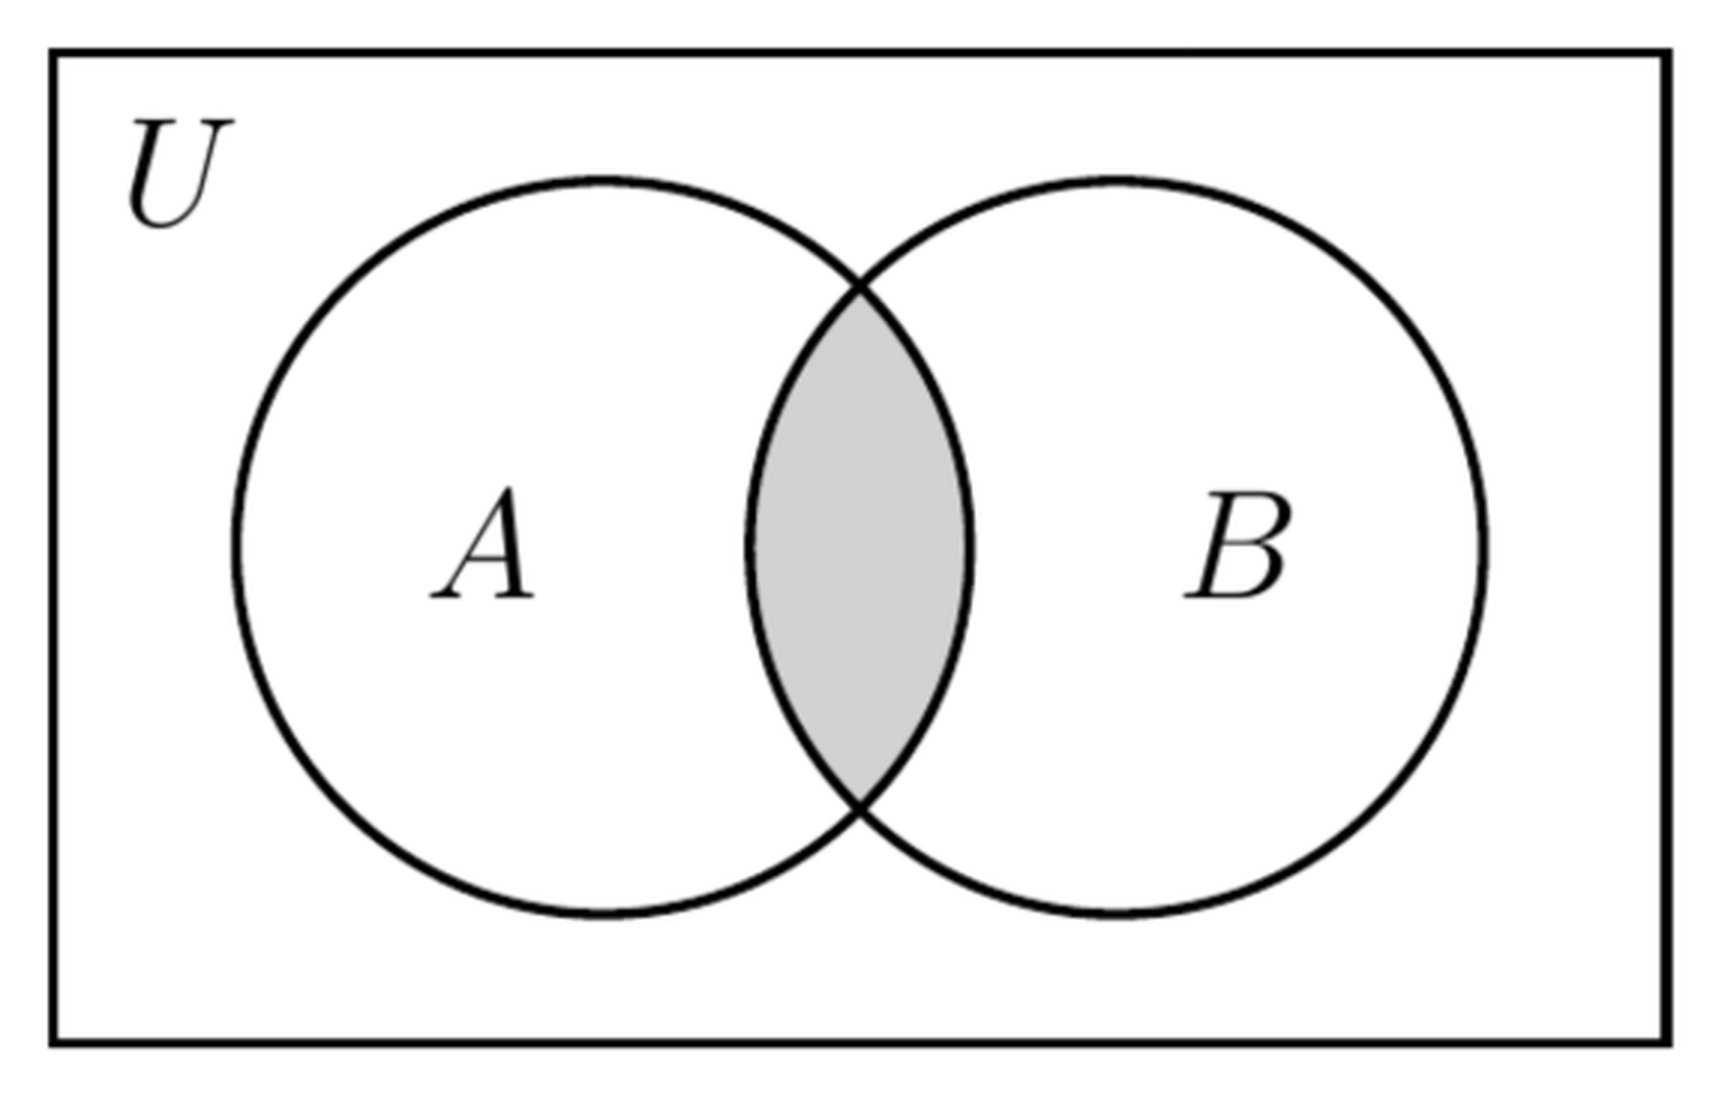
\includegraphics[width=0.38\textwidth]{figures/gao141_q5.png}
\end{center}

\ifanswer
\solbegin
\step{阴影部分表示 $A\cap B=\{4,7\}$.}
\solend
\fi

\item 方程 $2^{\log_3 x}=\dfrac12$ 的解集为\blankline[4.4em].

\ifanswer
\solbegin
\step{$2^{\log_3 x}=2^{-1}\Leftrightarrow\log_3 x=-1\Leftrightarrow x=\dfrac13$，解集为 $\left\{\dfrac13\right\}$.}
\solend
\fi

\item 若集合 $A=\left\{x\mid x^2+ax+\dfrac14=0\right\}$ 有且仅有两个子集，则实数 $a$ 的值为\blankline[4.4em].

\ifanswer
\solbegin
\step{$A$ 有且仅有两个子集，说明 $A$ 恰有一个元素，即方程有两个相等的实数根.}
\step{$\Delta=a^2-4\cdot\dfrac14=0\Rightarrow a=\pm1$.}% 判别式原卷印等腰偏高的高三角 $\Delta$，照录
\solend
\fi

\item 已知关于 $x$ 的方程 $x^2+mx+2m=0$ 的两个实数根分别为 $\alpha$、$\beta$，若 $\alpha^2+\beta^2=5$，则实数 $m=$\blankline[4.4em].

\ifanswer
\solbegin
\step{方程 $x^2+mx+2m=0$ 的两个实数根为 $\alpha$、$\beta$，}
\step{由根与系数的关系得 $\begin{cases}\alpha+\beta=-m\\\alpha\beta=2m\end{cases}$，又因为 $\alpha^2+\beta^2=5$，}
\step{所以 $\alpha^2+\beta^2=(\alpha+\beta)^2-2\alpha\beta=m^2-4m=5$，整理得 $m^2-4m-5=0$，}
\step{解得 $m=5$ 或 $m=-1$，}
\step{当 $m=5$ 时，$\triangle=25-40=-15<0$，无实根，舍去；}% 判别式原卷印扁等边三角 $\triangle$，照录
\step{当 $m=-1$ 时，$\triangle=1+8=9>0$，符合题意，}
\step{所以实数 $m=-1$.}
\solend
\fi

\item 若不等式 $\lvert x-3\rvert+\lvert x-5\rvert\geqslant a$ 对任意的实数 $x$ 恒成立，则实数 $a$ 的取值范围为\blankline[4.4em].

\ifanswer
\solbegin
\step{由三角不等式得 $\lvert x-3\rvert+\lvert x-5\rvert\geqslant\lvert x-3-x+5\rvert=2$，则 $a\leqslant2$.}
\solend
\fi

\item 设集合 $A=\{-3,2\}$，集合 $B=\{x\mid mx+1=0\}$，若 $A\cup B=A$，则实数 $m$ 的值为\blankline[4.4em].

\ifanswer
\solbegin
\step{由 $A\cup B=A$，得 $B\subseteq A$，}% 子集符号原卷印带下划线的 $\subseteq$，照录
\step{当 $m=0$ 时，$B=\varnothing$，满足题意，}
\step{当 $m\neq0$ 时，$B=\left\{-\dfrac1m\right\}$，所以 $-\dfrac1m=2$ 或 $-\dfrac1m=-3$，所以 $m=-\dfrac12$ 或 $m=\dfrac13$，}
\step{综上所述，$m=0$ 或 $m=-\dfrac12$ 或 $m=\dfrac13$.}
\solend
\fi

\item 已知 $m$ 为实数，代数式 $M=\sqrt{m-1}+\sqrt{3-m}$ 的取值范围为\blankline[4.4em].

\ifanswer
\solbegin
\step{根式有意义要求 $m\in[1,3]$，}
\step{此时 $(m-1)(3-m)=1-(m-2)^2$ 的取值范围为 $[0,1]$.}
\step{$M^2=2+2\sqrt{(m-1)(3-m)}$ 的取值范围为 $[2,4]$，又 $M>0$，}
\step{所以 $M\in[\sqrt2,2]$.}
\solend
\fi

\item 设有限集 $M$ 所含元素的个数用 $\mathbf{card}(M)$ 表示，并规定 $\mathbf{card}(\varnothing)=0$. 已知集合 $A,B$ 满足 $A\cup B=\{1,2,3\}$，$A\cap B=\varnothing$，若 $\mathbf{card}(A)\notin A$，$\mathbf{card}(B)\notin B$，则满足条件的所有不同集合 $A$ 的个数为\blankline[4.4em].

\ifanswer
\solbegin
\step{当 $\mathbf{card}(A)=0$ 或 $3$ 时，$A,B$ 中有一个为 $\{1,2,3\}$，不符合条件.}
\step{当 $\mathbf{card}(A)=1$ 时，$\mathbf{card}(B)=2\notin B$，所以 $A=\{2\}$，符合条件.}
\step{当 $\mathbf{card}(A)=2$ 时，$2\notin A$，所以 $B=\{2\}$，$A=\{1,3\}$，符合条件.}
\step{满足条件的集合 $A$ 共 $2$ 个.}
\solend
\fi

\end{enumerate}

\bigsec{二、选择题}

\begin{enumerate}
\setcounter{enumi}{12}

\item “ $x=1$ ” 是 “ $x^2-3x+2=0$ ” 的\mbox{（\quad）}条件.

\keepwithprev
A. 充分非必要\qquad B. 必要非充分

C. 充要\qquad D. 既非充分又非必要

\ifanswer
\solbegin
\step{$x^2-3x+2=0\Leftrightarrow x=1$ 或 $x=2$，所以 “ $x=1$ ” 是其充分非必要条件，}
\step{故选 $A$.}
\solend
\fi

\item 设 $a,b,c\in\R$，则下列命题为真命题的是\mbox{（\quad）}
% 原卷题干只声明 a,b,c，而 A 选项出现未声明的 d，照录（存疑）
\keepwithprev
A. 若 $a>b$ 且 $c>d$，则 $ac>bd$\qquad B. 若 $a^2>b^2$，则 $a>b$

C. 若 $ab>0$ 且 $a>b$，则 $\dfrac1a<\dfrac1b$\qquad D. 若 $a<0<b$，则 $\sqrt{-a}<\sqrt b$

\ifanswer
\solbegin
\step{$ab>0$ 且 $a>b\Rightarrow\dfrac1a-\dfrac1b=\dfrac{b-a}{ab}<0$，所以 $C$ 为真命题，故选 $C$.}
\solend
\fi

\item 已知 $\log_{14}7=a$，$14^b=5$，则 $\log_{35}28=$\mbox{（\quad）}

\keepwithprev
A. $\dfrac{2-a}{2a+b}$\qquad B. $\dfrac{2+a}{a+b}$\qquad C. $\dfrac{2-a}{a+2b}$\qquad D. $\dfrac{2-a}{a+b}$

\ifanswer
\solbegin
\step{$\log_{14}7=a$，$14^b=5$，}
\step{$\log_{35}28=\dfrac{\log_{14}28}{\log_{14}35}=\dfrac{\log_{14}14^2-\log_{14}7}{\log_{14}7+\log_{14}5}=\dfrac{2-a}{a+b}$. 故选 $D$.}
\solend
\fi

\item 关于 $x$ 的不等式 $ax^2+bx+3>0$ 的解集有下列说法，其中正确的个数是\mbox{（\quad）}

\keepwithprev
① 不等式 $ax^2+bx+3>0$ 的解集可以是 $\R$

② 不等式 $ax^2+bx+3>0$ 的解集可以是 $\{x\mid x>3\}$

③ 不等式 $ax^2+bx+3>0$ 的解集可以是 $\varnothing$

④ 不等式 $ax^2+bx+3>0$ 的解集可以是 $\{x\mid -1<x<3\}$

\keepwithprev
A. 4\qquad B. 3\qquad C. 2\qquad D. 1

\ifanswer
\solbegin
\step{$x=0$ 时左端为 $3>0$，解集必含 $0$，所以②③错误.}
\step{①取 $a=1,b=0$，$x^2+3>0$ 的解集为 $\R$，正确.}
\step{④取 $a=-1,b=2$，$-x^2+2x+3=-(x+1)(x-3)>0\Leftrightarrow-1<x<3$，正确.}
\step{正确的有①④，共 $2$ 个，故选 $C$.}
\solend
\fi

\end{enumerate}

\bigsec{三、解答题}

\begin{enumerate}
\setcounter{enumi}{16}

\item 已知集合 $A=\left\{x\mid\dfrac{x-2}{x+3}\geqslant0\right\}$，集合 $B=\{x\mid\lvert x+1\rvert+\lvert x-1\rvert<5\}$，全集 $U=\R$.

(1) 求 $A,B$；

(2) 求 $A\cup B$、$\overline{A\cap B}$.

\ifanswer
\solbegin
\step{(1) 分母不为零，且分子、分母同号或分子为零，}
\step{所以 $\dfrac{x-2}{x+3}\geqslant0\Leftrightarrow x<-3$ 或 $x\geqslant2$，因此 $A=(-\infty,-3)\cup[2,+\infty)$.}
\step{又 $\lvert x+1\rvert+\lvert x-1\rvert=\begin{cases}-2x,&x<-1\\2,&-1\leqslant x\leqslant1\\2x,&x>1\end{cases}$，}
\step{分别解得 $-\dfrac52<x<-1$、$-1\leqslant x\leqslant1$、$1<x<\dfrac52$，因此 $B=\left(-\dfrac52,\dfrac52\right)$.}
\step{(2) 合并两集合所对应的区间，得 $A\cup B=(-\infty,-3)\cup\left(-\dfrac52,+\infty\right)$，}
\step{两集合的公共部分为 $A\cap B=\left[2,\dfrac52\right)$，所以 $\overline{A\cap B}=(-\infty,2)\cup\left[\dfrac52,+\infty\right)$.}
\solend
\fi

\item (1) 已知 $a>b>0$，比较代数式 $\dfrac ab$ 与 $\dfrac{a+1}{b+1}$ 的大小并说明理由；

(2) 已知 $x,y,z$ 都是正实数，$a=x+\dfrac1y,b=y+\dfrac1z,c=z+\dfrac1x$，试用反证法证明 $a,b,c$ 至少有一个不小于 $2$.

\ifanswer
\solbegin
\step{(1) $\dfrac ab-\dfrac{a+1}{b+1}=\dfrac{a(b+1)-b(a+1)}{b(b+1)}=\dfrac{a-b}{b(b+1)}$，}
\step{因为 $a>b>0$，所以 $a-b>0$，$b(b+1)>0$，所以 $\dfrac ab-\dfrac{a+1}{b+1}>0$，}
\step{故 $\dfrac ab>\dfrac{a+1}{b+1}$.}
\step{(2) 假设 $a$、$b$、$c$ 三数都小于 $2$，则 $x+\dfrac1y+y+\dfrac1z+z+\dfrac1x<6$.}
\step{因为 $x,y,z$ 均大于 $0$，}
\step{所以 $x+\dfrac1y+y+\dfrac1z+z+\dfrac1x=x+\dfrac1x+y+\dfrac1y+z+\dfrac1z\geqslant2+2+2=6$，矛盾，}
\step{所以 $a$、$b$、$c$ 三数中至少有一个不小于 $2$.}
\solend
\fi

% 第 19 题长方体无盖贮水池砖墙示意图（题目配图，三版都出）：取原卷 06 页截图去粉色水印、LANCZOS 放大 3 倍
\needvspace{6cm}
\item 如图所示，某工厂要建造一个长方体形无盖贮水池，其容积为 $3200m^3$，深为 $2m$.

(1) 若水池的长比宽至少多 $60m$，求水池的宽的最大值；

(2) 若池底每平方米的造价为 $150$ 元，池壁每平方米的造价为 $120$ 元，那么怎样设计水池的长和宽能使总造价最低？最低总造价是多少？

\begin{center}
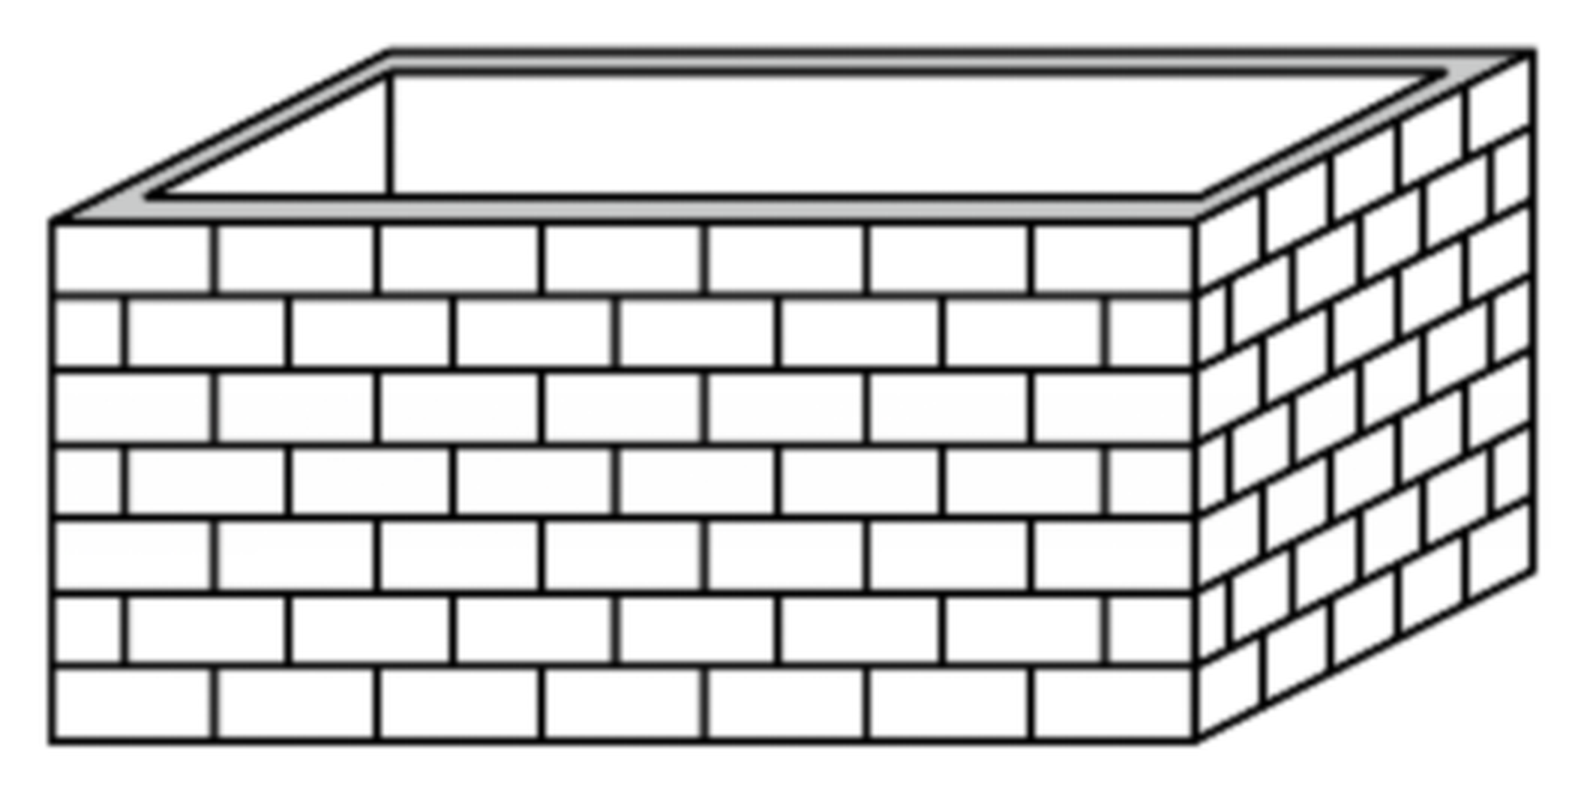
\includegraphics[width=0.42\textwidth]{figures/gao141_q19.png}
\end{center}

\ifanswer
\solbegin
\step{(1) 设水池的长、宽分别为 $xm$，$ym$，则 $x-y\geqslant60$，且 $x$、$y>0$，}
\step{由题意得 $2xy=3200$，即 $x=\dfrac{1600}{y}$，所以 $\dfrac{1600}{y}-y\geqslant60$，}
\step{因为 $y>0$，所以 $1600-y^2\geqslant60y$，}
\step{即 $y^2+60y-1600=(y+80)(y-20)\leqslant0$，解得 $-80\leqslant y\leqslant20$，}
\step{又 $y>0$，所以 $0<y\leqslant20$，所以水池的宽的最大值为 $20m$.}
\step{(2) 设水池总造价为 $z$ 元，}
\step{则 $z=1600\times150+2\times(2x+2y)\times120=240000+480(x+y)$，}
\step{又因为 $y=\dfrac{1600}{x}$，}
\step{所以 $z=240000+\left(x+\dfrac{1600}{x}\right)\times480\geqslant240000+480\times2\sqrt{1600}$}
\step{$=240000+38400=278400$，}
\step{当且仅当 $x=\dfrac{1600}{x}$，即 $x=y=40$ 时取等号，}
\step{所以，将水池的池底设计为边长为 $40m$ 的正方形时总造价最低，}
\step{最低总造价为 $278400$ 元.}
\solend
\fi

\item 已知 $a\in\R$，设集合 $A=\{x\mid ax^2-3x+2<ax-1\}$.

(1) 若 $A=(1,3)$，求实数 $a$ 的值；

(2) 当 $a>0$ 时，求 $A$；

(3) 若 “ $x\in\left(\dfrac12,+\infty\right)$ ” 是 “ $x\in A$ ” 的必要非充分条件，求实数 $a$ 的取值范围.

\ifanswer
\solbegin
\step{原不等式等价于 $ax^2-(a+3)x+3<0\Leftrightarrow(x-1)(ax-3)<0$，}
\step{(1) $A=(1,3)$ 为有界区间，因此 $a>0$，两根为 $1$ 和 $\dfrac3a$，于是 $\dfrac3a=3$，得 $a=1$；}
\step{此时 $(x-1)(x-3)<0$ 的解集确为 $(1,3)$.}
\step{(2) 当 $a>0$ 时，二次项系数为正，比较 $1$ 与 $\dfrac3a$，得 $A=\begin{cases}\left(1,\dfrac3a\right),&0<a<3\\\varnothing,&a=3\\\left(\dfrac3a,1\right),&a>3\end{cases}$，}
\step{其中 $a=3$ 时，原不等式为 $3(x-1)^2<0$，无解.}
\step{(3) 记 $S=\left(\dfrac12,+\infty\right)$，题意要求 $A\subset S$.}% 子集符号原卷印单线 $\subset$，照录
\step{由于对任意 $a$ 都有 $1\notin A$，而 $1\in S$，所以只需满足 $A\subseteq S$.}
\step{当 $a<0$ 时，$A=\left(-\infty,\dfrac3a\right)\cup(1,+\infty)$，含有小于 $\dfrac12$ 的数，不符合条件.}
\step{当 $a=0$ 时，$A=(1,+\infty)$，符合条件.}
\step{当 $0<a<3$ 时，$A=\left(1,\dfrac3a\right)\subseteq S$；}
\step{当 $a=3$ 时，$A=\varnothing\subseteq S$，均符合条件；}
\step{当 $a>3$ 时，$A=\left(\dfrac3a,1\right)$，所以 $A\subseteq S\Leftrightarrow\dfrac3a\geqslant\dfrac12\Leftrightarrow a\leqslant6$；}
\step{因此实数 $a$ 的取值范围为 $[0,6]$.}
\solend
\fi

\item 甲、乙两同学探讨了一个问题：已知正实数 $x,y$ 满足 $3x+y=1$，求 $\dfrac1x+\dfrac1y$ 的最小值.

甲给出的解法：由 $1=3x+y\geqslant2\sqrt{3xy}$，得 $\sqrt{xy}\leqslant\dfrac{\sqrt3}{6}$，所以 $\dfrac1x+\dfrac1y\geqslant2\sqrt{\dfrac1{xy}}\geqslant4\sqrt3$. 因此 $\dfrac1x+\dfrac1y$ 的最小值为 $4\sqrt3$.

乙给出的解法：$\dfrac1x+\dfrac1y=\left(\dfrac1x+\dfrac1y\right)(3x+y)=4+\dfrac yx+\dfrac{3x}{y}$，因为 $x,y$ 均为正实数，所以 $\dfrac1x+\dfrac1y\geqslant4+2\sqrt{\dfrac yx\cdot\dfrac{3x}{y}}=4+2\sqrt3$.

(1) 请判断上述哪位同学的解法正确，哪位同学的解法错误，并指出错误的原因；

(2) 结合上述探讨，试求当 $0<x<\dfrac12$ 时，$\dfrac1x+\dfrac1{1-2x}$ 的最小值以及此时实数 $x$ 的值；

(3) 已知 $x$ 为正实数，$y$ 为非负实数，且 $x+2y=2$，求 $\dfrac{x^2+1}{x}+\dfrac{2y^2}{y+1}$ 的最小值以及此时实数 $x,y$ 的值.

\ifanswer
\solbegin
\step{(1) 甲的推导中，$3x+y\geqslant2\sqrt{3xy}$ 取等号要求 $3x=y$，}
\step{$\dfrac1x+\dfrac1y\geqslant\dfrac2{\sqrt{xy}}$ 取等号要求 $x=y$，两者对正实数 $x,y$ 不能同时成立，}
\step{因此不能将 $4\sqrt3$ 判为最小值，甲错误.}
\step{乙的等号条件为 $\dfrac yx=\dfrac{3x}{y}$，即 $y=\sqrt3 x$；}
\step{结合 $3x+y=1$，得 $x=\dfrac1{3+\sqrt3},y=\dfrac{\sqrt3}{3+\sqrt3}$ 均为正数，等号可以成立，}
\step{因此乙正确，最小值为 $4+2\sqrt3$.}
\step{(2) 令 $t=1-2x>0$，则 $2x+t=1$.}
\step{$\dfrac1x+\dfrac1t=\left(\dfrac1x+\dfrac1t\right)(2x+t)=3+\dfrac tx+\dfrac{2x}{t}\geqslant3+2\sqrt2$，}
\step{当且仅当 $\dfrac tx=\dfrac{2x}{t}$，即 $t=\sqrt2 x$ 时取等号，}
\step{由 $2x+t=1$，得 $x=\dfrac1{2+\sqrt2}=\dfrac{2-\sqrt2}{2}\in\left(0,\dfrac12\right)$，}
\step{因此最小值为 $3+2\sqrt2$，此时 $x=\dfrac{2-\sqrt2}{2}$.}
\step{(3) 记目标式为 $F$，利用 $x+2y=2$，}
\step{得 $F=x+\dfrac1x+2y-2+\dfrac2{y+1}=\dfrac1x+\dfrac2{y+1}$，}
\step{又 $x+2(y+1)=4$，且 $x>0$、$y+1>0$，}
\step{所以 $4F=\left(\dfrac1x+\dfrac2{y+1}\right)(x+2(y+1))=5+2\left(\dfrac{y+1}{x}+\dfrac{x}{y+1}\right)$}
\step{$\geqslant5+2\times2=9$，当且仅当 $\dfrac{y+1}{x}=\dfrac{x}{y+1}$，即 $x=y+1$ 时取等号.}
\step{联立 $x+2y=2$，得 $x=\dfrac43$、$y=\dfrac13$，满足题设条件，}
\step{因此最小值为 $\dfrac94$，此时 $x=\dfrac43$，$y=\dfrac13$.}
\solend
\fi

\end{enumerate}

\end{document}
"
%
% ① 原始材料：微信公众号"魔都数学加油站"文章，连载"27学年高一141"，原文标题
% "27学年高一141——2026-2027年上海市彭浦中学高一上期中"；
% 原文链接：https://mp.weixin.qq.com/s/V_8bEhC6geeFyQysmtqUtQ。
% 正文为 9 张 PNG 页（01、05、06、07、09 为 2560x3620；02、03、04、08 为 4762x6735，
% 同一篇各页分辨率不同，逐页按各自分辨率放大裁图核对），题目下印【解析】，为讲评版。
% 题目、解析均据原图转录；卷面粉红色水印"魔都数学加油站"及公众号页脚未录入。
% 全卷 2 幅插图，均属题目配图（在 \ifanswer 外、三版都出）、取原卷截图去粉色水印、
% LANCZOS 放大 3 倍：第 5 题韦恩图（01 页，全集 U 矩形内两圆相交、交集阴影、A/B/U 标注）、
% 第 19 题长方体无盖贮水池砖墙示意图（06 页右上）。通读 9 页确认除这 2 幅外无其它
% 插图/表格，亦无"题干写如图而源码漏图"（仅 Q5"图中阴影部分"、Q19"如图所示"两处提到图）。
%
% 卷首标题：原卷印作"2026-2027 年彭浦中学高一上期中"（公众号标题中的"上海市"
% 卷面标题行没有，本稿照卷面），年份区间按全稿惯例排 en dash；原卷未印副标题，
% 本卷为期中卷、跨集合与常用逻辑用语／不等式／函数三章，按题目内容补出
% "集合与常用逻辑用语、不等式、函数"（与 高一140 同期中卷口径相同）：
% 集合与逻辑见 Q5、Q10、Q12、Q13、Q16、Q17、Q20，不等式见 Q4、Q9、Q14、Q18、
% Q19、Q21，函数（指数／对数）见 Q6、Q15。
%
% 题号体例：本卷共 19 题——一、填空题 3—12（10 题）、二、选择题 13—16（4 题）、
% 三、解答题 17—21（5 题）。三节分别 \setcounter{enumi}{2}／{12}／{16}。
% 原卷从第 3 题起、无第 1、2 题，本稿保留原题号；全卷无附加题节。
%
% ② 与原卷的排版差异：
%   ① 原文从第 3 题起，本稿保留原题号；
%   ② 原卷 19 题题下均印【解析】，无独立【答案】段、无"答案印题干括号且无解析"、
%      无"只印【答案】无解析"一型：填空题与解答题的答案落在【解析】末句
%      （Q3—Q12、Q17—Q21），四道选择题答案在【解析】末句"故选 …"
%      （Q13 选 A、Q14 选 C、Q15 选 D、Q16 选 C），题干括号内一律留空；
%      本稿 19 题一律 \solbegin…\solend、全卷不提 \ans{}，答案版【解析】标记数
%      = 19 = 全卷题数（无【答案】标记）；
%   ③ 原卷未印副标题，本稿按"知识模块"口径补出；
%   ④ 原卷填空横线按全稿惯例排 \blankline[4.4em]；选择题括号排 \mbox{（\quad）}，
%      选项段／命题段前按惯例加 \keepwithprev（Q16 两枚：命题列与选项段各一）；
%      解答题不留作答区、不加 \anspace（原卷为讲评版，与 129／131／132／133／136／140 同）；
%   ⑤ 原卷数集混排：黑板粗体 R（Q14 题干、Q16 ① 与解析、Q17 全集、Q20 题干）
%      按全稿惯例统一改 \R；空集记号 \varnothing；绝对值排 \lvert…\rvert，
%      集合描述竖线排 \mid；不等号按全稿惯例排 \leqslant／\geqslant；
%      补集照原卷上划线排 \overline{A\cap B}（Q17(2) 题干与解析）；
%      原卷"card"记号排黑体正体（Q12），本稿照录 \mathbf{card}，未改斜体
%      （与 高一66 同题口径不同：那份原卷 card 排斜体、照录 $card(M)$）；
%   ⑥ 子题标号 (1)(2)(3) 原卷印半角括号，照录；圈数字 ①②③④ 在正文（文本模式）
%      按原卷照录，未进数学式；数学式内半角逗号照录（如 Q12"$A,B$"、"{1,2,3}"、
%      Q14"$a,b,c\in\R$"、Q15"$\log_{14}7=a$，$14^b=5$"、Q16"$a=1,b=0$"、
%      Q18"$x,y,z$"、Q20"$x,y$"、Q21"$x,y$"）；全卷行末西文句点照录为 ASCII 句点；
%      行中全角逗号、顿号照录；
%   ⑦ 题干中的中文弯引号按原卷照录（Q13、Q20(3) 的 “ ” 及引号内空格），
%      注释内一律 ASCII 引号；
%   ⑧ 两幅题目配图各在 \item 之前加 \needvspace 守卫整块推走（Q5 5cm、Q19 6cm），
%      守卫放在 \item 之前而非 \bigsec 之后——两题均非各节首题，不触发 B 类
%      "节标题落页末"（照 高一26／40／59／136／140 成例）；三版切页审计均"合计异常：无"；
%   ⑨ 跨页续印按题合并：Q8 题干与【解析】首行在 01 页、后 6 行在 02 页；
%      Q15 题干在 03 页、【解析】在 04 页；Q17 题干与【解析】前 2 行在 04 页、
%      后 4 行在 05 页；Q19 题干在 05 页末、(1)(2) 小问与砖墙图与【解析】在 06 页；
%      Q20 题干 (1)(2) 在 06 页末、(3) 与【解析】在 07 页；Q21 题干与【解析】
%      前 6 行在 08 页、后 12 行在 09 页；Q16、Q18 全在各自页内；
%      本稿按题连排，不丢行；
%   ⑩ 原卷无红色加粗标签（【解析】均黑色印刷，Q16 解析 "①取…""④取…" 与
%      Q20 解析 "(2)" 等分步标签亦黑色），故本卷未用 \stepm；
%   ⑪ 原卷 Q19 题干把数值与单位（3200m³、2m、60m、150 元、120 元、40m、20m、
%      278400 元）印作略粗的西文字形，本稿按全稿惯例（高一70／72 同类题）排普通
%      数学体，未加粗。
%
% ③ 行数复核：一条 \step = 原卷解析的一个印刷行，cases 块作一个印刷行计。逐题数 \step
%   条数，合计 92 条（Q3：1；Q4：1；Q5：1；Q6：1；Q7：2；Q8：7；Q9：1；Q10：4；
%   Q11：4；Q12：4；Q13：2；Q14：1；Q15：2；Q16：4；Q17：6；Q18：7；Q19：13；
%   Q20：13；Q21：18），与原卷印刷行逐题相等。全卷 19 题均印【解析】、无独立 \ans{}，
%   答案版【解析】标记数 = 19 = 全卷题数。
%
% ④ 判别式／子集符号结论（逐处放大原图照录、不得统一）：
%   判别式：全卷 3 处——第 7 题【解析】"$\Delta=a^2-4\cdot\frac14=0$"一处原卷印
%     等腰、偏高的高三角 $\Delta$，照录 \Delta；第 8 题【解析】
%     "$\triangle=25-40=-15<0$"与"$\triangle=1+8=9>0$"两处原卷印扁等边三角
%     $\triangle$，照录 \triangle。两形不同，逐处照录未统一。
%   子集：全卷 6 处——第 10 题【解析】"$B\subseteq A$"一处、第 20 题【解析】
%     "所以只需满足 $A\subseteq S$"、"$A=\left(1,\frac3a\right)\subseteq S$"、
%     "$A=\varnothing\subseteq S$"、"$A\subseteq S\Leftrightarrow\frac3a\geqslant\frac12$"
%     四处，共 5 处原卷印带下划线的 $\subseteq$，照录 \subseteq；第 20 题【解析】
%     (3) 首行"题意要求 $A\subset S$"一处原卷印单线 $\subset$，照录 \subset
%     （下行因 $1\in S$ 而 $1\notin A$，改述为 $A\subseteq S$，两者逻辑一致、非笔误）。
%
% ⑤ 存疑照录（照录未改，正文对应处另有 % 注）：
%   第 14 题题干"设 $a,b,c\in\R$"只声明 $a,b,c$，而 A 选项"若 $a>b$ 且 $c>d$，
%     则 $ac>bd$"引入未声明的 $d$，原卷变量声明与选项不统一，照录未补。
%   全卷除此 1 条外未发现其它笔误／自相矛盾处。
%
% ⑥ 跨页续印按题合并说明：见 ② ⑨。
%
\documentclass[a4paper,11pt]{article}
\usepackage{common}

\begin{document}

\examtitlest[3]{2026--2027 年彭浦中学高一上期中}{集合与常用逻辑用语、不等式、函数}

\bigsec{一、填空题}

\begin{enumerate}
\setcounter{enumi}{2}

\item 已知 $m$ 为实数，若 $1\in\{m,m^2\}$，则 $m$ 的值为\blankline[4.4em].

\ifanswer
\solbegin
\step{$m=1$ 或 $m^2=1$，得 $m=\pm1$；按列举项互异口径排除 $m=m^2=1$，得 $m=-1$.}
\solend
\fi

\item 已知 $2<a<4$，$-2<b<1$，则 $2a+b$ 的取值范围为\blankline[4.4em].

\ifanswer
\solbegin
\step{$4<2a<8$，与 $-2<b<1$ 相加，得 $2<2a+b<9$，取值范围为 $(2,9)$.}
\solend
\fi

% 第 5 题韦恩图（题目配图，三版都出）：取原卷 01 页截图去粉色水印、LANCZOS 放大 3 倍
\needvspace{5cm}
\item 已知集合 $A=\{-1,-2,1,4,7\}$，$B=\{x\mid x>1\}$，用列举法表示图中阴影部分所表示的集合为\blankline[4.4em].

\begin{center}
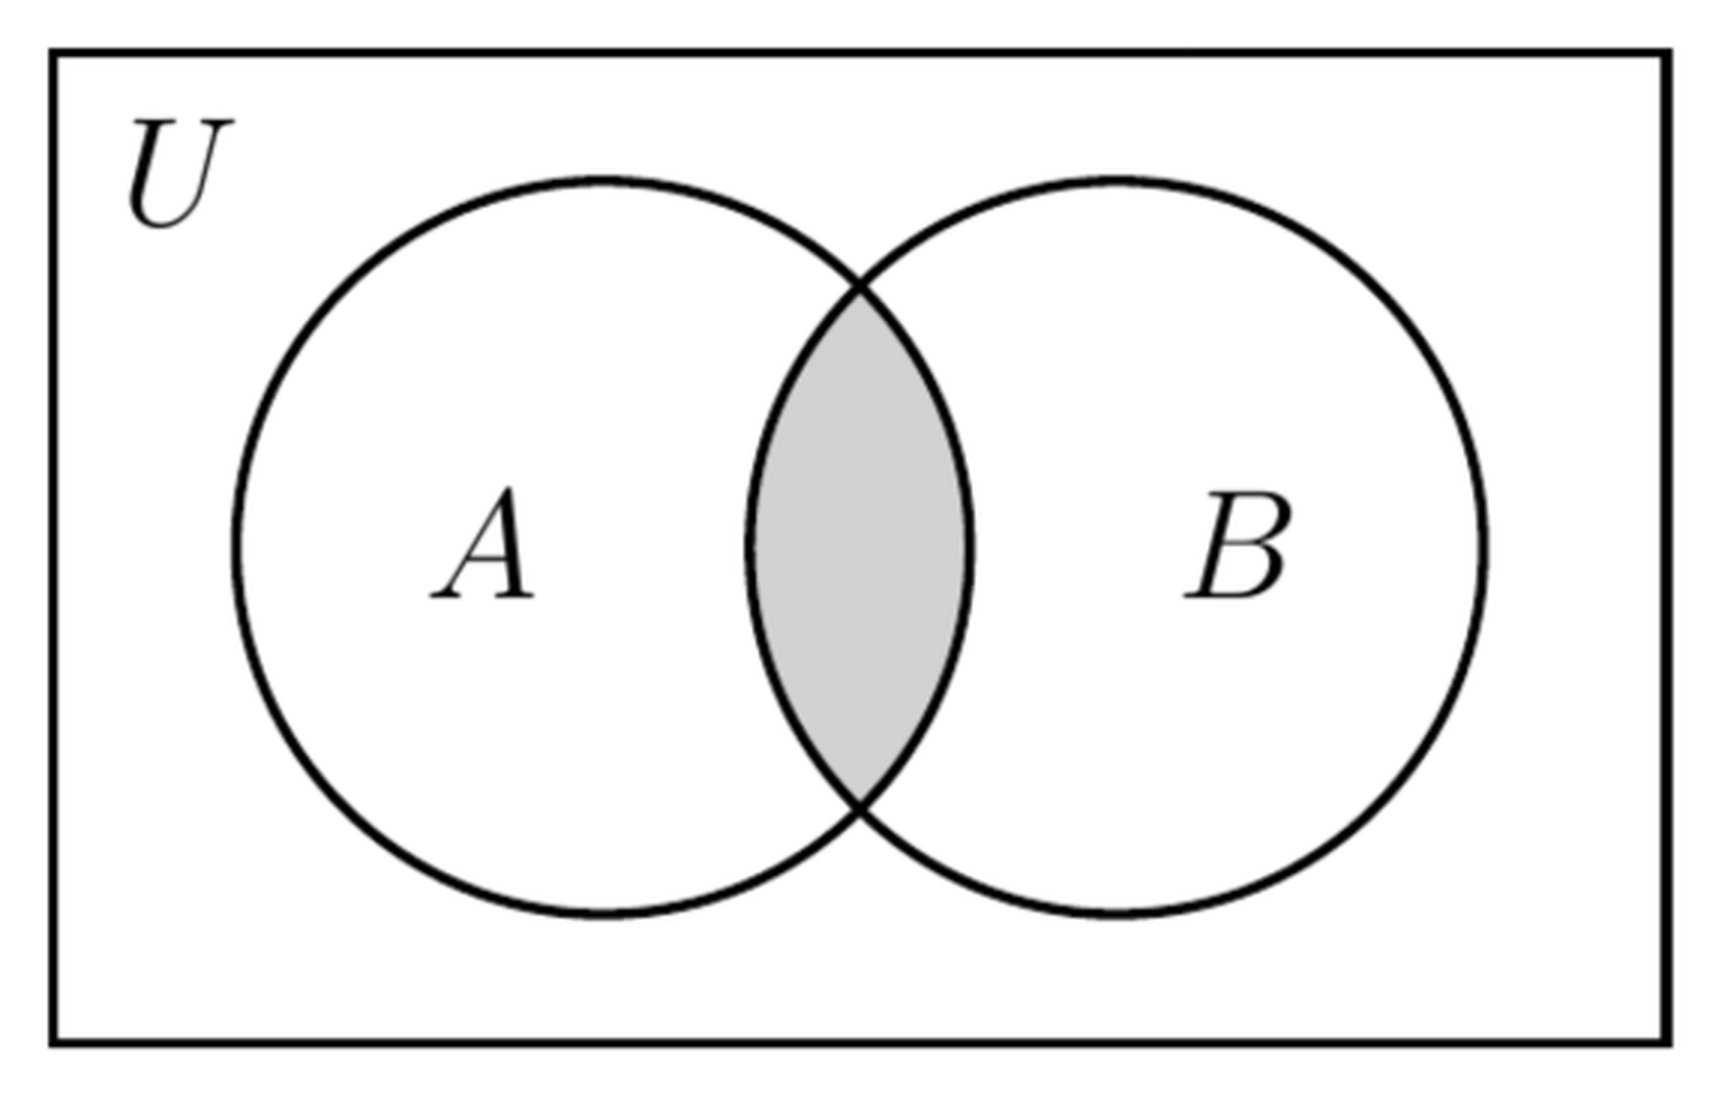
\includegraphics[width=0.38\textwidth]{figures/gao141_q5.png}
\end{center}

\ifanswer
\solbegin
\step{阴影部分表示 $A\cap B=\{4,7\}$.}
\solend
\fi

\item 方程 $2^{\log_3 x}=\dfrac12$ 的解集为\blankline[4.4em].

\ifanswer
\solbegin
\step{$2^{\log_3 x}=2^{-1}\Leftrightarrow\log_3 x=-1\Leftrightarrow x=\dfrac13$，解集为 $\left\{\dfrac13\right\}$.}
\solend
\fi

\item 若集合 $A=\left\{x\mid x^2+ax+\dfrac14=0\right\}$ 有且仅有两个子集，则实数 $a$ 的值为\blankline[4.4em].

\ifanswer
\solbegin
\step{$A$ 有且仅有两个子集，说明 $A$ 恰有一个元素，即方程有两个相等的实数根.}
\step{$\Delta=a^2-4\cdot\dfrac14=0\Rightarrow a=\pm1$.}% 判别式原卷印等腰偏高的高三角 $\Delta$，照录
\solend
\fi

\item 已知关于 $x$ 的方程 $x^2+mx+2m=0$ 的两个实数根分别为 $\alpha$、$\beta$，若 $\alpha^2+\beta^2=5$，则实数 $m=$\blankline[4.4em].

\ifanswer
\solbegin
\step{方程 $x^2+mx+2m=0$ 的两个实数根为 $\alpha$、$\beta$，}
\step{由根与系数的关系得 $\begin{cases}\alpha+\beta=-m\\\alpha\beta=2m\end{cases}$，又因为 $\alpha^2+\beta^2=5$，}
\step{所以 $\alpha^2+\beta^2=(\alpha+\beta)^2-2\alpha\beta=m^2-4m=5$，整理得 $m^2-4m-5=0$，}
\step{解得 $m=5$ 或 $m=-1$，}
\step{当 $m=5$ 时，$\triangle=25-40=-15<0$，无实根，舍去；}% 判别式原卷印扁等边三角 $\triangle$，照录
\step{当 $m=-1$ 时，$\triangle=1+8=9>0$，符合题意，}
\step{所以实数 $m=-1$.}
\solend
\fi

\item 若不等式 $\lvert x-3\rvert+\lvert x-5\rvert\geqslant a$ 对任意的实数 $x$ 恒成立，则实数 $a$ 的取值范围为\blankline[4.4em].

\ifanswer
\solbegin
\step{由三角不等式得 $\lvert x-3\rvert+\lvert x-5\rvert\geqslant\lvert x-3-x+5\rvert=2$，则 $a\leqslant2$.}
\solend
\fi

\item 设集合 $A=\{-3,2\}$，集合 $B=\{x\mid mx+1=0\}$，若 $A\cup B=A$，则实数 $m$ 的值为\blankline[4.4em].

\ifanswer
\solbegin
\step{由 $A\cup B=A$，得 $B\subseteq A$，}% 子集符号原卷印带下划线的 $\subseteq$，照录
\step{当 $m=0$ 时，$B=\varnothing$，满足题意，}
\step{当 $m\neq0$ 时，$B=\left\{-\dfrac1m\right\}$，所以 $-\dfrac1m=2$ 或 $-\dfrac1m=-3$，所以 $m=-\dfrac12$ 或 $m=\dfrac13$，}
\step{综上所述，$m=0$ 或 $m=-\dfrac12$ 或 $m=\dfrac13$.}
\solend
\fi

\item 已知 $m$ 为实数，代数式 $M=\sqrt{m-1}+\sqrt{3-m}$ 的取值范围为\blankline[4.4em].

\ifanswer
\solbegin
\step{根式有意义要求 $m\in[1,3]$，}
\step{此时 $(m-1)(3-m)=1-(m-2)^2$ 的取值范围为 $[0,1]$.}
\step{$M^2=2+2\sqrt{(m-1)(3-m)}$ 的取值范围为 $[2,4]$，又 $M>0$，}
\step{所以 $M\in[\sqrt2,2]$.}
\solend
\fi

\item 设有限集 $M$ 所含元素的个数用 $\mathbf{card}(M)$ 表示，并规定 $\mathbf{card}(\varnothing)=0$. 已知集合 $A,B$ 满足 $A\cup B=\{1,2,3\}$，$A\cap B=\varnothing$，若 $\mathbf{card}(A)\notin A$，$\mathbf{card}(B)\notin B$，则满足条件的所有不同集合 $A$ 的个数为\blankline[4.4em].

\ifanswer
\solbegin
\step{当 $\mathbf{card}(A)=0$ 或 $3$ 时，$A,B$ 中有一个为 $\{1,2,3\}$，不符合条件.}
\step{当 $\mathbf{card}(A)=1$ 时，$\mathbf{card}(B)=2\notin B$，所以 $A=\{2\}$，符合条件.}
\step{当 $\mathbf{card}(A)=2$ 时，$2\notin A$，所以 $B=\{2\}$，$A=\{1,3\}$，符合条件.}
\step{满足条件的集合 $A$ 共 $2$ 个.}
\solend
\fi

\end{enumerate}

\bigsec{二、选择题}

\begin{enumerate}
\setcounter{enumi}{12}

\item “ $x=1$ ” 是 “ $x^2-3x+2=0$ ” 的\mbox{（\quad）}条件.

\keepwithprev
A. 充分非必要\qquad B. 必要非充分

C. 充要\qquad D. 既非充分又非必要

\ifanswer
\solbegin
\step{$x^2-3x+2=0\Leftrightarrow x=1$ 或 $x=2$，所以 “ $x=1$ ” 是其充分非必要条件，}
\step{故选 $A$.}
\solend
\fi

\item 设 $a,b,c\in\R$，则下列命题为真命题的是\mbox{（\quad）}
% 原卷题干只声明 a,b,c，而 A 选项出现未声明的 d，照录（存疑）
\keepwithprev
A. 若 $a>b$ 且 $c>d$，则 $ac>bd$\qquad B. 若 $a^2>b^2$，则 $a>b$

C. 若 $ab>0$ 且 $a>b$，则 $\dfrac1a<\dfrac1b$\qquad D. 若 $a<0<b$，则 $\sqrt{-a}<\sqrt b$

\ifanswer
\solbegin
\step{$ab>0$ 且 $a>b\Rightarrow\dfrac1a-\dfrac1b=\dfrac{b-a}{ab}<0$，所以 $C$ 为真命题，故选 $C$.}
\solend
\fi

\item 已知 $\log_{14}7=a$，$14^b=5$，则 $\log_{35}28=$\mbox{（\quad）}

\keepwithprev
A. $\dfrac{2-a}{2a+b}$\qquad B. $\dfrac{2+a}{a+b}$\qquad C. $\dfrac{2-a}{a+2b}$\qquad D. $\dfrac{2-a}{a+b}$

\ifanswer
\solbegin
\step{$\log_{14}7=a$，$14^b=5$，}
\step{$\log_{35}28=\dfrac{\log_{14}28}{\log_{14}35}=\dfrac{\log_{14}14^2-\log_{14}7}{\log_{14}7+\log_{14}5}=\dfrac{2-a}{a+b}$. 故选 $D$.}
\solend
\fi

\item 关于 $x$ 的不等式 $ax^2+bx+3>0$ 的解集有下列说法，其中正确的个数是\mbox{（\quad）}

\keepwithprev
① 不等式 $ax^2+bx+3>0$ 的解集可以是 $\R$

② 不等式 $ax^2+bx+3>0$ 的解集可以是 $\{x\mid x>3\}$

③ 不等式 $ax^2+bx+3>0$ 的解集可以是 $\varnothing$

④ 不等式 $ax^2+bx+3>0$ 的解集可以是 $\{x\mid -1<x<3\}$

\keepwithprev
A. 4\qquad B. 3\qquad C. 2\qquad D. 1

\ifanswer
\solbegin
\step{$x=0$ 时左端为 $3>0$，解集必含 $0$，所以②③错误.}
\step{①取 $a=1,b=0$，$x^2+3>0$ 的解集为 $\R$，正确.}
\step{④取 $a=-1,b=2$，$-x^2+2x+3=-(x+1)(x-3)>0\Leftrightarrow-1<x<3$，正确.}
\step{正确的有①④，共 $2$ 个，故选 $C$.}
\solend
\fi

\end{enumerate}

\bigsec{三、解答题}

\begin{enumerate}
\setcounter{enumi}{16}

\item 已知集合 $A=\left\{x\mid\dfrac{x-2}{x+3}\geqslant0\right\}$，集合 $B=\{x\mid\lvert x+1\rvert+\lvert x-1\rvert<5\}$，全集 $U=\R$.

(1) 求 $A,B$；

(2) 求 $A\cup B$、$\overline{A\cap B}$.

\ifanswer
\solbegin
\step{(1) 分母不为零，且分子、分母同号或分子为零，}
\step{所以 $\dfrac{x-2}{x+3}\geqslant0\Leftrightarrow x<-3$ 或 $x\geqslant2$，因此 $A=(-\infty,-3)\cup[2,+\infty)$.}
\step{又 $\lvert x+1\rvert+\lvert x-1\rvert=\begin{cases}-2x,&x<-1\\2,&-1\leqslant x\leqslant1\\2x,&x>1\end{cases}$，}
\step{分别解得 $-\dfrac52<x<-1$、$-1\leqslant x\leqslant1$、$1<x<\dfrac52$，因此 $B=\left(-\dfrac52,\dfrac52\right)$.}
\step{(2) 合并两集合所对应的区间，得 $A\cup B=(-\infty,-3)\cup\left(-\dfrac52,+\infty\right)$，}
\step{两集合的公共部分为 $A\cap B=\left[2,\dfrac52\right)$，所以 $\overline{A\cap B}=(-\infty,2)\cup\left[\dfrac52,+\infty\right)$.}
\solend
\fi

\item (1) 已知 $a>b>0$，比较代数式 $\dfrac ab$ 与 $\dfrac{a+1}{b+1}$ 的大小并说明理由；

(2) 已知 $x,y,z$ 都是正实数，$a=x+\dfrac1y,b=y+\dfrac1z,c=z+\dfrac1x$，试用反证法证明 $a,b,c$ 至少有一个不小于 $2$.

\ifanswer
\solbegin
\step{(1) $\dfrac ab-\dfrac{a+1}{b+1}=\dfrac{a(b+1)-b(a+1)}{b(b+1)}=\dfrac{a-b}{b(b+1)}$，}
\step{因为 $a>b>0$，所以 $a-b>0$，$b(b+1)>0$，所以 $\dfrac ab-\dfrac{a+1}{b+1}>0$，}
\step{故 $\dfrac ab>\dfrac{a+1}{b+1}$.}
\step{(2) 假设 $a$、$b$、$c$ 三数都小于 $2$，则 $x+\dfrac1y+y+\dfrac1z+z+\dfrac1x<6$.}
\step{因为 $x,y,z$ 均大于 $0$，}
\step{所以 $x+\dfrac1y+y+\dfrac1z+z+\dfrac1x=x+\dfrac1x+y+\dfrac1y+z+\dfrac1z\geqslant2+2+2=6$，矛盾，}
\step{所以 $a$、$b$、$c$ 三数中至少有一个不小于 $2$.}
\solend
\fi

% 第 19 题长方体无盖贮水池砖墙示意图（题目配图，三版都出）：取原卷 06 页截图去粉色水印、LANCZOS 放大 3 倍
\needvspace{6cm}
\item 如图所示，某工厂要建造一个长方体形无盖贮水池，其容积为 $3200m^3$，深为 $2m$.

(1) 若水池的长比宽至少多 $60m$，求水池的宽的最大值；

(2) 若池底每平方米的造价为 $150$ 元，池壁每平方米的造价为 $120$ 元，那么怎样设计水池的长和宽能使总造价最低？最低总造价是多少？

\begin{center}
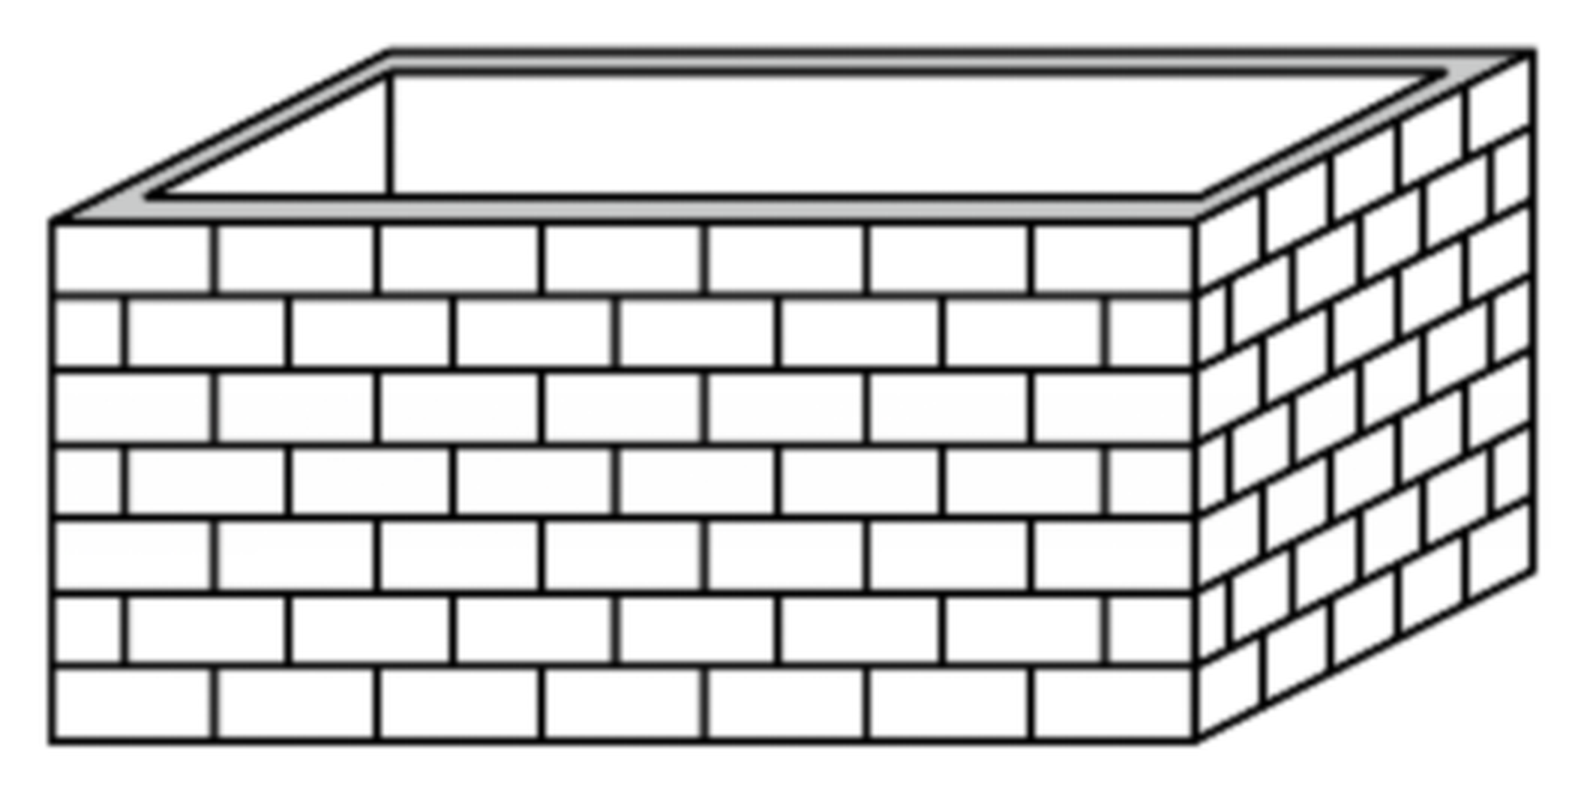
\includegraphics[width=0.42\textwidth]{figures/gao141_q19.png}
\end{center}

\ifanswer
\solbegin
\step{(1) 设水池的长、宽分别为 $xm$，$ym$，则 $x-y\geqslant60$，且 $x$、$y>0$，}
\step{由题意得 $2xy=3200$，即 $x=\dfrac{1600}{y}$，所以 $\dfrac{1600}{y}-y\geqslant60$，}
\step{因为 $y>0$，所以 $1600-y^2\geqslant60y$，}
\step{即 $y^2+60y-1600=(y+80)(y-20)\leqslant0$，解得 $-80\leqslant y\leqslant20$，}
\step{又 $y>0$，所以 $0<y\leqslant20$，所以水池的宽的最大值为 $20m$.}
\step{(2) 设水池总造价为 $z$ 元，}
\step{则 $z=1600\times150+2\times(2x+2y)\times120=240000+480(x+y)$，}
\step{又因为 $y=\dfrac{1600}{x}$，}
\step{所以 $z=240000+\left(x+\dfrac{1600}{x}\right)\times480\geqslant240000+480\times2\sqrt{1600}$}
\step{$=240000+38400=278400$，}
\step{当且仅当 $x=\dfrac{1600}{x}$，即 $x=y=40$ 时取等号，}
\step{所以，将水池的池底设计为边长为 $40m$ 的正方形时总造价最低，}
\step{最低总造价为 $278400$ 元.}
\solend
\fi

\item 已知 $a\in\R$，设集合 $A=\{x\mid ax^2-3x+2<ax-1\}$.

(1) 若 $A=(1,3)$，求实数 $a$ 的值；

(2) 当 $a>0$ 时，求 $A$；

(3) 若 “ $x\in\left(\dfrac12,+\infty\right)$ ” 是 “ $x\in A$ ” 的必要非充分条件，求实数 $a$ 的取值范围.

\ifanswer
\solbegin
\step{原不等式等价于 $ax^2-(a+3)x+3<0\Leftrightarrow(x-1)(ax-3)<0$，}
\step{(1) $A=(1,3)$ 为有界区间，因此 $a>0$，两根为 $1$ 和 $\dfrac3a$，于是 $\dfrac3a=3$，得 $a=1$；}
\step{此时 $(x-1)(x-3)<0$ 的解集确为 $(1,3)$.}
\step{(2) 当 $a>0$ 时，二次项系数为正，比较 $1$ 与 $\dfrac3a$，得 $A=\begin{cases}\left(1,\dfrac3a\right),&0<a<3\\\varnothing,&a=3\\\left(\dfrac3a,1\right),&a>3\end{cases}$，}
\step{其中 $a=3$ 时，原不等式为 $3(x-1)^2<0$，无解.}
\step{(3) 记 $S=\left(\dfrac12,+\infty\right)$，题意要求 $A\subset S$.}% 子集符号原卷印单线 $\subset$，照录
\step{由于对任意 $a$ 都有 $1\notin A$，而 $1\in S$，所以只需满足 $A\subseteq S$.}
\step{当 $a<0$ 时，$A=\left(-\infty,\dfrac3a\right)\cup(1,+\infty)$，含有小于 $\dfrac12$ 的数，不符合条件.}
\step{当 $a=0$ 时，$A=(1,+\infty)$，符合条件.}
\step{当 $0<a<3$ 时，$A=\left(1,\dfrac3a\right)\subseteq S$；}
\step{当 $a=3$ 时，$A=\varnothing\subseteq S$，均符合条件；}
\step{当 $a>3$ 时，$A=\left(\dfrac3a,1\right)$，所以 $A\subseteq S\Leftrightarrow\dfrac3a\geqslant\dfrac12\Leftrightarrow a\leqslant6$；}
\step{因此实数 $a$ 的取值范围为 $[0,6]$.}
\solend
\fi

\item 甲、乙两同学探讨了一个问题：已知正实数 $x,y$ 满足 $3x+y=1$，求 $\dfrac1x+\dfrac1y$ 的最小值.

甲给出的解法：由 $1=3x+y\geqslant2\sqrt{3xy}$，得 $\sqrt{xy}\leqslant\dfrac{\sqrt3}{6}$，所以 $\dfrac1x+\dfrac1y\geqslant2\sqrt{\dfrac1{xy}}\geqslant4\sqrt3$. 因此 $\dfrac1x+\dfrac1y$ 的最小值为 $4\sqrt3$.

乙给出的解法：$\dfrac1x+\dfrac1y=\left(\dfrac1x+\dfrac1y\right)(3x+y)=4+\dfrac yx+\dfrac{3x}{y}$，因为 $x,y$ 均为正实数，所以 $\dfrac1x+\dfrac1y\geqslant4+2\sqrt{\dfrac yx\cdot\dfrac{3x}{y}}=4+2\sqrt3$.

(1) 请判断上述哪位同学的解法正确，哪位同学的解法错误，并指出错误的原因；

(2) 结合上述探讨，试求当 $0<x<\dfrac12$ 时，$\dfrac1x+\dfrac1{1-2x}$ 的最小值以及此时实数 $x$ 的值；

(3) 已知 $x$ 为正实数，$y$ 为非负实数，且 $x+2y=2$，求 $\dfrac{x^2+1}{x}+\dfrac{2y^2}{y+1}$ 的最小值以及此时实数 $x,y$ 的值.

\ifanswer
\solbegin
\step{(1) 甲的推导中，$3x+y\geqslant2\sqrt{3xy}$ 取等号要求 $3x=y$，}
\step{$\dfrac1x+\dfrac1y\geqslant\dfrac2{\sqrt{xy}}$ 取等号要求 $x=y$，两者对正实数 $x,y$ 不能同时成立，}
\step{因此不能将 $4\sqrt3$ 判为最小值，甲错误.}
\step{乙的等号条件为 $\dfrac yx=\dfrac{3x}{y}$，即 $y=\sqrt3 x$；}
\step{结合 $3x+y=1$，得 $x=\dfrac1{3+\sqrt3},y=\dfrac{\sqrt3}{3+\sqrt3}$ 均为正数，等号可以成立，}
\step{因此乙正确，最小值为 $4+2\sqrt3$.}
\step{(2) 令 $t=1-2x>0$，则 $2x+t=1$.}
\step{$\dfrac1x+\dfrac1t=\left(\dfrac1x+\dfrac1t\right)(2x+t)=3+\dfrac tx+\dfrac{2x}{t}\geqslant3+2\sqrt2$，}
\step{当且仅当 $\dfrac tx=\dfrac{2x}{t}$，即 $t=\sqrt2 x$ 时取等号，}
\step{由 $2x+t=1$，得 $x=\dfrac1{2+\sqrt2}=\dfrac{2-\sqrt2}{2}\in\left(0,\dfrac12\right)$，}
\step{因此最小值为 $3+2\sqrt2$，此时 $x=\dfrac{2-\sqrt2}{2}$.}
\step{(3) 记目标式为 $F$，利用 $x+2y=2$，}
\step{得 $F=x+\dfrac1x+2y-2+\dfrac2{y+1}=\dfrac1x+\dfrac2{y+1}$，}
\step{又 $x+2(y+1)=4$，且 $x>0$、$y+1>0$，}
\step{所以 $4F=\left(\dfrac1x+\dfrac2{y+1}\right)(x+2(y+1))=5+2\left(\dfrac{y+1}{x}+\dfrac{x}{y+1}\right)$}
\step{$\geqslant5+2\times2=9$，当且仅当 $\dfrac{y+1}{x}=\dfrac{x}{y+1}$，即 $x=y+1$ 时取等号.}
\step{联立 $x+2y=2$，得 $x=\dfrac43$、$y=\dfrac13$，满足题设条件，}
\step{因此最小值为 $\dfrac94$，此时 $x=\dfrac43$，$y=\dfrac13$.}
\solend
\fi

\end{enumerate}

\end{document}
"
%
% ① 原始材料：微信公众号"魔都数学加油站"文章，连载"27学年高一141"，原文标题
% "27学年高一141——2026-2027年上海市彭浦中学高一上期中"；
% 原文链接：https://mp.weixin.qq.com/s/V_8bEhC6geeFyQysmtqUtQ。
% 正文为 9 张 PNG 页（01、05、06、07、09 为 2560x3620；02、03、04、08 为 4762x6735，
% 同一篇各页分辨率不同，逐页按各自分辨率放大裁图核对），题目下印【解析】，为讲评版。
% 题目、解析均据原图转录；卷面粉红色水印"魔都数学加油站"及公众号页脚未录入。
% 全卷 2 幅插图，均属题目配图（在 \ifanswer 外、三版都出）、取原卷截图去粉色水印、
% LANCZOS 放大 3 倍：第 5 题韦恩图（01 页，全集 U 矩形内两圆相交、交集阴影、A/B/U 标注）、
% 第 19 题长方体无盖贮水池砖墙示意图（06 页右上）。通读 9 页确认除这 2 幅外无其它
% 插图/表格，亦无"题干写如图而源码漏图"（仅 Q5"图中阴影部分"、Q19"如图所示"两处提到图）。
%
% 卷首标题：原卷印作"2026-2027 年彭浦中学高一上期中"（公众号标题中的"上海市"
% 卷面标题行没有，本稿照卷面），年份区间按全稿惯例排 en dash；原卷未印副标题，
% 本卷为期中卷、跨集合与常用逻辑用语／不等式／函数三章，按题目内容补出
% "集合与常用逻辑用语、不等式、函数"（与 高一140 同期中卷口径相同）：
% 集合与逻辑见 Q5、Q10、Q12、Q13、Q16、Q17、Q20，不等式见 Q4、Q9、Q14、Q18、
% Q19、Q21，函数（指数／对数）见 Q6、Q15。
%
% 题号体例：本卷共 19 题——一、填空题 3—12（10 题）、二、选择题 13—16（4 题）、
% 三、解答题 17—21（5 题）。三节分别 \setcounter{enumi}{2}／{12}／{16}。
% 原卷从第 3 题起、无第 1、2 题，本稿保留原题号；全卷无附加题节。
%
% ② 与原卷的排版差异：
%   ① 原文从第 3 题起，本稿保留原题号；
%   ② 原卷 19 题题下均印【解析】，无独立【答案】段、无"答案印题干括号且无解析"、
%      无"只印【答案】无解析"一型：填空题与解答题的答案落在【解析】末句
%      （Q3—Q12、Q17—Q21），四道选择题答案在【解析】末句"故选 …"
%      （Q13 选 A、Q14 选 C、Q15 选 D、Q16 选 C），题干括号内一律留空；
%      本稿 19 题一律 \solbegin…\solend、全卷不提 \ans{}，答案版【解析】标记数
%      = 19 = 全卷题数（无【答案】标记）；
%   ③ 原卷未印副标题，本稿按"知识模块"口径补出；
%   ④ 原卷填空横线按全稿惯例排 \blankline[4.4em]；选择题括号排 \mbox{（\quad）}，
%      选项段／命题段前按惯例加 \keepwithprev（Q16 两枚：命题列与选项段各一）；
%      解答题不留作答区、不加 \anspace（原卷为讲评版，与 129／131／132／133／136／140 同）；
%   ⑤ 原卷数集混排：黑板粗体 R（Q14 题干、Q16 ① 与解析、Q17 全集、Q20 题干）
%      按全稿惯例统一改 \R；空集记号 \varnothing；绝对值排 \lvert…\rvert，
%      集合描述竖线排 \mid；不等号按全稿惯例排 \leqslant／\geqslant；
%      补集照原卷上划线排 \overline{A\cap B}（Q17(2) 题干与解析）；
%      原卷"card"记号排黑体正体（Q12），本稿照录 \mathbf{card}，未改斜体
%      （与 高一66 同题口径不同：那份原卷 card 排斜体、照录 $card(M)$）；
%   ⑥ 子题标号 (1)(2)(3) 原卷印半角括号，照录；圈数字 ①②③④ 在正文（文本模式）
%      按原卷照录，未进数学式；数学式内半角逗号照录（如 Q12"$A,B$"、"{1,2,3}"、
%      Q14"$a,b,c\in\R$"、Q15"$\log_{14}7=a$，$14^b=5$"、Q16"$a=1,b=0$"、
%      Q18"$x,y,z$"、Q20"$x,y$"、Q21"$x,y$"）；全卷行末西文句点照录为 ASCII 句点；
%      行中全角逗号、顿号照录；
%   ⑦ 题干中的中文弯引号按原卷照录（Q13、Q20(3) 的 “ ” 及引号内空格），
%      注释内一律 ASCII 引号；
%   ⑧ 两幅题目配图各在 \item 之前加 \needvspace 守卫整块推走（Q5 5cm、Q19 6cm），
%      守卫放在 \item 之前而非 \bigsec 之后——两题均非各节首题，不触发 B 类
%      "节标题落页末"（照 高一26／40／59／136／140 成例）；三版切页审计均"合计异常：无"；
%   ⑨ 跨页续印按题合并：Q8 题干与【解析】首行在 01 页、后 6 行在 02 页；
%      Q15 题干在 03 页、【解析】在 04 页；Q17 题干与【解析】前 2 行在 04 页、
%      后 4 行在 05 页；Q19 题干在 05 页末、(1)(2) 小问与砖墙图与【解析】在 06 页；
%      Q20 题干 (1)(2) 在 06 页末、(3) 与【解析】在 07 页；Q21 题干与【解析】
%      前 6 行在 08 页、后 12 行在 09 页；Q16、Q18 全在各自页内；
%      本稿按题连排，不丢行；
%   ⑩ 原卷无红色加粗标签（【解析】均黑色印刷，Q16 解析 "①取…""④取…" 与
%      Q20 解析 "(2)" 等分步标签亦黑色），故本卷未用 \stepm；
%   ⑪ 原卷 Q19 题干把数值与单位（3200m³、2m、60m、150 元、120 元、40m、20m、
%      278400 元）印作略粗的西文字形，本稿按全稿惯例（高一70／72 同类题）排普通
%      数学体，未加粗。
%
% ③ 行数复核：一条 \step = 原卷解析的一个印刷行，cases 块作一个印刷行计。逐题数 \step
%   条数，合计 92 条（Q3：1；Q4：1；Q5：1；Q6：1；Q7：2；Q8：7；Q9：1；Q10：4；
%   Q11：4；Q12：4；Q13：2；Q14：1；Q15：2；Q16：4；Q17：6；Q18：7；Q19：13；
%   Q20：13；Q21：18），与原卷印刷行逐题相等。全卷 19 题均印【解析】、无独立 \ans{}，
%   答案版【解析】标记数 = 19 = 全卷题数。
%
% ④ 判别式／子集符号结论（逐处放大原图照录、不得统一）：
%   判别式：全卷 3 处——第 7 题【解析】"$\Delta=a^2-4\cdot\frac14=0$"一处原卷印
%     等腰、偏高的高三角 $\Delta$，照录 \Delta；第 8 题【解析】
%     "$\triangle=25-40=-15<0$"与"$\triangle=1+8=9>0$"两处原卷印扁等边三角
%     $\triangle$，照录 \triangle。两形不同，逐处照录未统一。
%   子集：全卷 6 处——第 10 题【解析】"$B\subseteq A$"一处、第 20 题【解析】
%     "所以只需满足 $A\subseteq S$"、"$A=\left(1,\frac3a\right)\subseteq S$"、
%     "$A=\varnothing\subseteq S$"、"$A\subseteq S\Leftrightarrow\frac3a\geqslant\frac12$"
%     四处，共 5 处原卷印带下划线的 $\subseteq$，照录 \subseteq；第 20 题【解析】
%     (3) 首行"题意要求 $A\subset S$"一处原卷印单线 $\subset$，照录 \subset
%     （下行因 $1\in S$ 而 $1\notin A$，改述为 $A\subseteq S$，两者逻辑一致、非笔误）。
%
% ⑤ 存疑照录（照录未改，正文对应处另有 % 注）：
%   第 14 题题干"设 $a,b,c\in\R$"只声明 $a,b,c$，而 A 选项"若 $a>b$ 且 $c>d$，
%     则 $ac>bd$"引入未声明的 $d$，原卷变量声明与选项不统一，照录未补。
%   全卷除此 1 条外未发现其它笔误／自相矛盾处。
%
% ⑥ 跨页续印按题合并说明：见 ② ⑨。
%
\documentclass[a4paper,11pt]{article}
\usepackage{common}

\begin{document}

\examtitlest[3]{2026--2027 年彭浦中学高一上期中}{集合与常用逻辑用语、不等式、函数}

\bigsec{一、填空题}

\begin{enumerate}
\setcounter{enumi}{2}

\item 已知 $m$ 为实数，若 $1\in\{m,m^2\}$，则 $m$ 的值为\blankline[4.4em].

\ifanswer
\solbegin
\step{$m=1$ 或 $m^2=1$，得 $m=\pm1$；按列举项互异口径排除 $m=m^2=1$，得 $m=-1$.}
\solend
\fi

\item 已知 $2<a<4$，$-2<b<1$，则 $2a+b$ 的取值范围为\blankline[4.4em].

\ifanswer
\solbegin
\step{$4<2a<8$，与 $-2<b<1$ 相加，得 $2<2a+b<9$，取值范围为 $(2,9)$.}
\solend
\fi

% 第 5 题韦恩图（题目配图，三版都出）：取原卷 01 页截图去粉色水印、LANCZOS 放大 3 倍
\needvspace{5cm}
\item 已知集合 $A=\{-1,-2,1,4,7\}$，$B=\{x\mid x>1\}$，用列举法表示图中阴影部分所表示的集合为\blankline[4.4em].

\begin{center}
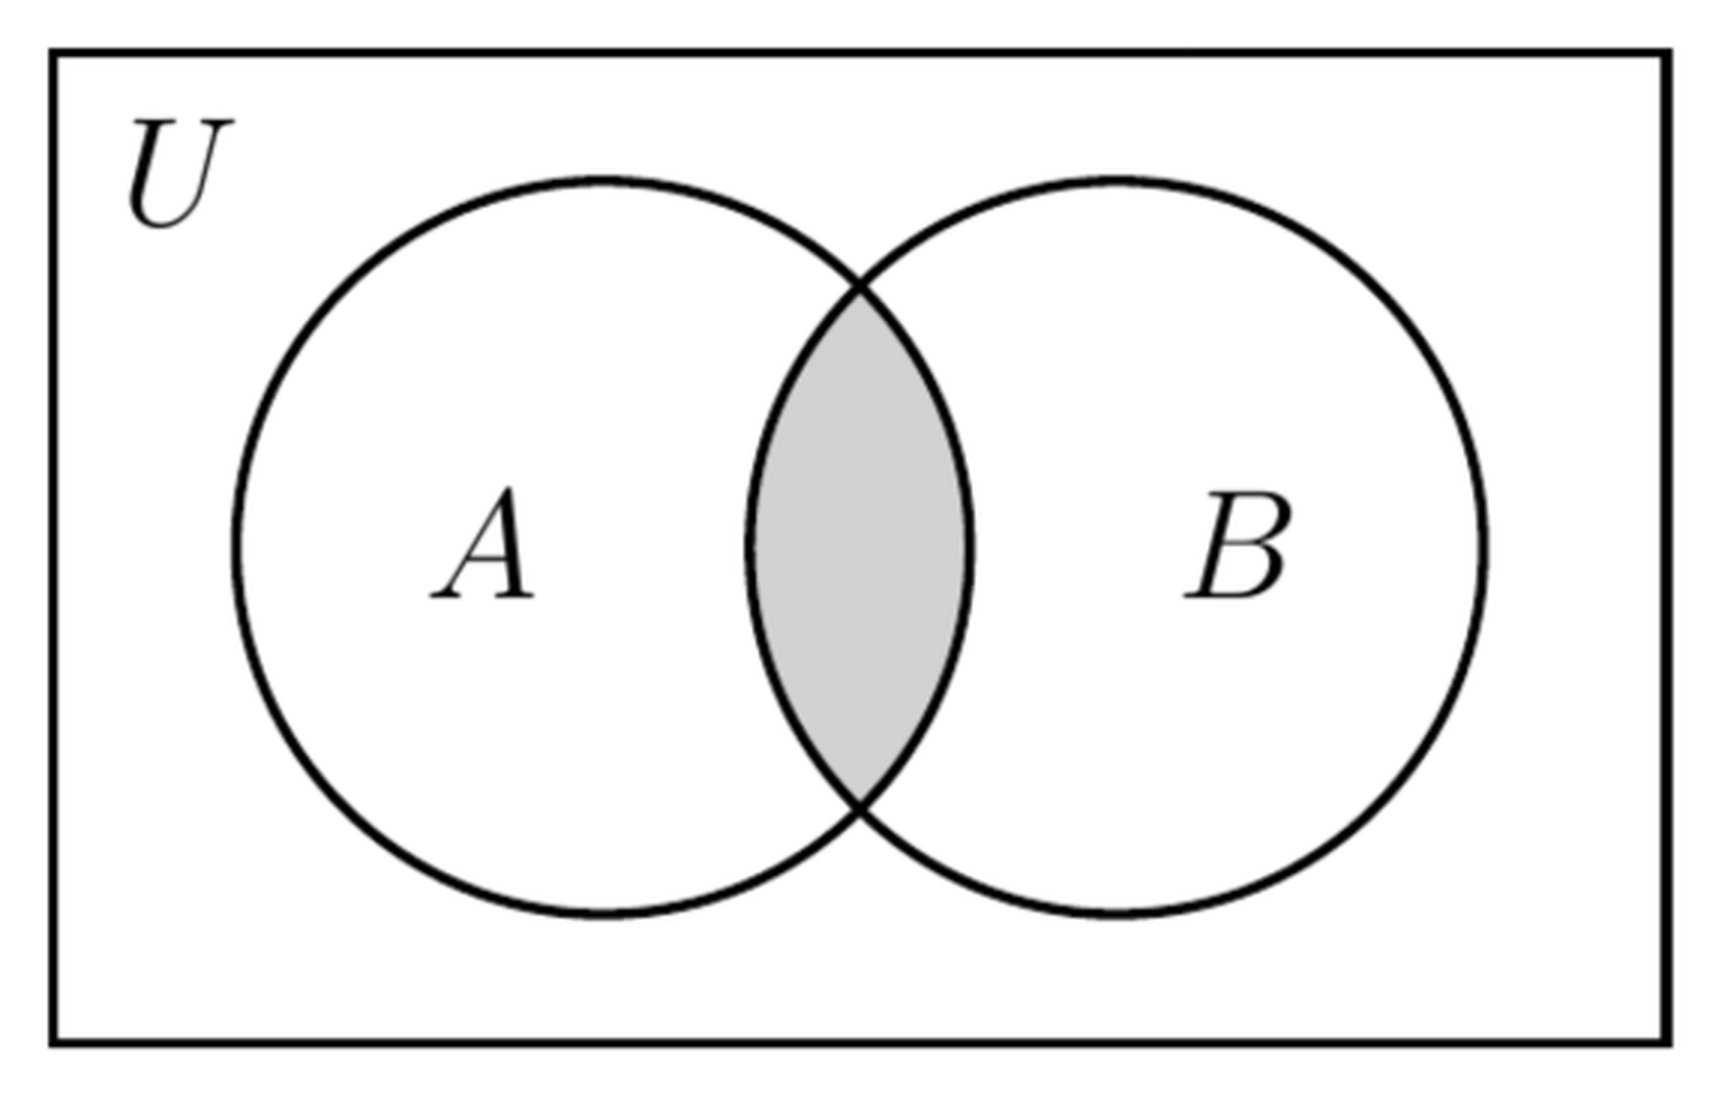
\includegraphics[width=0.38\textwidth]{figures/gao141_q5.png}
\end{center}

\ifanswer
\solbegin
\step{阴影部分表示 $A\cap B=\{4,7\}$.}
\solend
\fi

\item 方程 $2^{\log_3 x}=\dfrac12$ 的解集为\blankline[4.4em].

\ifanswer
\solbegin
\step{$2^{\log_3 x}=2^{-1}\Leftrightarrow\log_3 x=-1\Leftrightarrow x=\dfrac13$，解集为 $\left\{\dfrac13\right\}$.}
\solend
\fi

\item 若集合 $A=\left\{x\mid x^2+ax+\dfrac14=0\right\}$ 有且仅有两个子集，则实数 $a$ 的值为\blankline[4.4em].

\ifanswer
\solbegin
\step{$A$ 有且仅有两个子集，说明 $A$ 恰有一个元素，即方程有两个相等的实数根.}
\step{$\Delta=a^2-4\cdot\dfrac14=0\Rightarrow a=\pm1$.}% 判别式原卷印等腰偏高的高三角 $\Delta$，照录
\solend
\fi

\item 已知关于 $x$ 的方程 $x^2+mx+2m=0$ 的两个实数根分别为 $\alpha$、$\beta$，若 $\alpha^2+\beta^2=5$，则实数 $m=$\blankline[4.4em].

\ifanswer
\solbegin
\step{方程 $x^2+mx+2m=0$ 的两个实数根为 $\alpha$、$\beta$，}
\step{由根与系数的关系得 $\begin{cases}\alpha+\beta=-m\\\alpha\beta=2m\end{cases}$，又因为 $\alpha^2+\beta^2=5$，}
\step{所以 $\alpha^2+\beta^2=(\alpha+\beta)^2-2\alpha\beta=m^2-4m=5$，整理得 $m^2-4m-5=0$，}
\step{解得 $m=5$ 或 $m=-1$，}
\step{当 $m=5$ 时，$\triangle=25-40=-15<0$，无实根，舍去；}% 判别式原卷印扁等边三角 $\triangle$，照录
\step{当 $m=-1$ 时，$\triangle=1+8=9>0$，符合题意，}
\step{所以实数 $m=-1$.}
\solend
\fi

\item 若不等式 $\lvert x-3\rvert+\lvert x-5\rvert\geqslant a$ 对任意的实数 $x$ 恒成立，则实数 $a$ 的取值范围为\blankline[4.4em].

\ifanswer
\solbegin
\step{由三角不等式得 $\lvert x-3\rvert+\lvert x-5\rvert\geqslant\lvert x-3-x+5\rvert=2$，则 $a\leqslant2$.}
\solend
\fi

\item 设集合 $A=\{-3,2\}$，集合 $B=\{x\mid mx+1=0\}$，若 $A\cup B=A$，则实数 $m$ 的值为\blankline[4.4em].

\ifanswer
\solbegin
\step{由 $A\cup B=A$，得 $B\subseteq A$，}% 子集符号原卷印带下划线的 $\subseteq$，照录
\step{当 $m=0$ 时，$B=\varnothing$，满足题意，}
\step{当 $m\neq0$ 时，$B=\left\{-\dfrac1m\right\}$，所以 $-\dfrac1m=2$ 或 $-\dfrac1m=-3$，所以 $m=-\dfrac12$ 或 $m=\dfrac13$，}
\step{综上所述，$m=0$ 或 $m=-\dfrac12$ 或 $m=\dfrac13$.}
\solend
\fi

\item 已知 $m$ 为实数，代数式 $M=\sqrt{m-1}+\sqrt{3-m}$ 的取值范围为\blankline[4.4em].

\ifanswer
\solbegin
\step{根式有意义要求 $m\in[1,3]$，}
\step{此时 $(m-1)(3-m)=1-(m-2)^2$ 的取值范围为 $[0,1]$.}
\step{$M^2=2+2\sqrt{(m-1)(3-m)}$ 的取值范围为 $[2,4]$，又 $M>0$，}
\step{所以 $M\in[\sqrt2,2]$.}
\solend
\fi

\item 设有限集 $M$ 所含元素的个数用 $\mathbf{card}(M)$ 表示，并规定 $\mathbf{card}(\varnothing)=0$. 已知集合 $A,B$ 满足 $A\cup B=\{1,2,3\}$，$A\cap B=\varnothing$，若 $\mathbf{card}(A)\notin A$，$\mathbf{card}(B)\notin B$，则满足条件的所有不同集合 $A$ 的个数为\blankline[4.4em].

\ifanswer
\solbegin
\step{当 $\mathbf{card}(A)=0$ 或 $3$ 时，$A,B$ 中有一个为 $\{1,2,3\}$，不符合条件.}
\step{当 $\mathbf{card}(A)=1$ 时，$\mathbf{card}(B)=2\notin B$，所以 $A=\{2\}$，符合条件.}
\step{当 $\mathbf{card}(A)=2$ 时，$2\notin A$，所以 $B=\{2\}$，$A=\{1,3\}$，符合条件.}
\step{满足条件的集合 $A$ 共 $2$ 个.}
\solend
\fi

\end{enumerate}

\bigsec{二、选择题}

\begin{enumerate}
\setcounter{enumi}{12}

\item “ $x=1$ ” 是 “ $x^2-3x+2=0$ ” 的\mbox{（\quad）}条件.

\keepwithprev
A. 充分非必要\qquad B. 必要非充分

C. 充要\qquad D. 既非充分又非必要

\ifanswer
\solbegin
\step{$x^2-3x+2=0\Leftrightarrow x=1$ 或 $x=2$，所以 “ $x=1$ ” 是其充分非必要条件，}
\step{故选 $A$.}
\solend
\fi

\item 设 $a,b,c\in\R$，则下列命题为真命题的是\mbox{（\quad）}
% 原卷题干只声明 a,b,c，而 A 选项出现未声明的 d，照录（存疑）
\keepwithprev
A. 若 $a>b$ 且 $c>d$，则 $ac>bd$\qquad B. 若 $a^2>b^2$，则 $a>b$

C. 若 $ab>0$ 且 $a>b$，则 $\dfrac1a<\dfrac1b$\qquad D. 若 $a<0<b$，则 $\sqrt{-a}<\sqrt b$

\ifanswer
\solbegin
\step{$ab>0$ 且 $a>b\Rightarrow\dfrac1a-\dfrac1b=\dfrac{b-a}{ab}<0$，所以 $C$ 为真命题，故选 $C$.}
\solend
\fi

\item 已知 $\log_{14}7=a$，$14^b=5$，则 $\log_{35}28=$\mbox{（\quad）}

\keepwithprev
A. $\dfrac{2-a}{2a+b}$\qquad B. $\dfrac{2+a}{a+b}$\qquad C. $\dfrac{2-a}{a+2b}$\qquad D. $\dfrac{2-a}{a+b}$

\ifanswer
\solbegin
\step{$\log_{14}7=a$，$14^b=5$，}
\step{$\log_{35}28=\dfrac{\log_{14}28}{\log_{14}35}=\dfrac{\log_{14}14^2-\log_{14}7}{\log_{14}7+\log_{14}5}=\dfrac{2-a}{a+b}$. 故选 $D$.}
\solend
\fi

\item 关于 $x$ 的不等式 $ax^2+bx+3>0$ 的解集有下列说法，其中正确的个数是\mbox{（\quad）}

\keepwithprev
① 不等式 $ax^2+bx+3>0$ 的解集可以是 $\R$

② 不等式 $ax^2+bx+3>0$ 的解集可以是 $\{x\mid x>3\}$

③ 不等式 $ax^2+bx+3>0$ 的解集可以是 $\varnothing$

④ 不等式 $ax^2+bx+3>0$ 的解集可以是 $\{x\mid -1<x<3\}$

\keepwithprev
A. 4\qquad B. 3\qquad C. 2\qquad D. 1

\ifanswer
\solbegin
\step{$x=0$ 时左端为 $3>0$，解集必含 $0$，所以②③错误.}
\step{①取 $a=1,b=0$，$x^2+3>0$ 的解集为 $\R$，正确.}
\step{④取 $a=-1,b=2$，$-x^2+2x+3=-(x+1)(x-3)>0\Leftrightarrow-1<x<3$，正确.}
\step{正确的有①④，共 $2$ 个，故选 $C$.}
\solend
\fi

\end{enumerate}

\bigsec{三、解答题}

\begin{enumerate}
\setcounter{enumi}{16}

\item 已知集合 $A=\left\{x\mid\dfrac{x-2}{x+3}\geqslant0\right\}$，集合 $B=\{x\mid\lvert x+1\rvert+\lvert x-1\rvert<5\}$，全集 $U=\R$.

(1) 求 $A,B$；

(2) 求 $A\cup B$、$\overline{A\cap B}$.

\ifanswer
\solbegin
\step{(1) 分母不为零，且分子、分母同号或分子为零，}
\step{所以 $\dfrac{x-2}{x+3}\geqslant0\Leftrightarrow x<-3$ 或 $x\geqslant2$，因此 $A=(-\infty,-3)\cup[2,+\infty)$.}
\step{又 $\lvert x+1\rvert+\lvert x-1\rvert=\begin{cases}-2x,&x<-1\\2,&-1\leqslant x\leqslant1\\2x,&x>1\end{cases}$，}
\step{分别解得 $-\dfrac52<x<-1$、$-1\leqslant x\leqslant1$、$1<x<\dfrac52$，因此 $B=\left(-\dfrac52,\dfrac52\right)$.}
\step{(2) 合并两集合所对应的区间，得 $A\cup B=(-\infty,-3)\cup\left(-\dfrac52,+\infty\right)$，}
\step{两集合的公共部分为 $A\cap B=\left[2,\dfrac52\right)$，所以 $\overline{A\cap B}=(-\infty,2)\cup\left[\dfrac52,+\infty\right)$.}
\solend
\fi

\item (1) 已知 $a>b>0$，比较代数式 $\dfrac ab$ 与 $\dfrac{a+1}{b+1}$ 的大小并说明理由；

(2) 已知 $x,y,z$ 都是正实数，$a=x+\dfrac1y,b=y+\dfrac1z,c=z+\dfrac1x$，试用反证法证明 $a,b,c$ 至少有一个不小于 $2$.

\ifanswer
\solbegin
\step{(1) $\dfrac ab-\dfrac{a+1}{b+1}=\dfrac{a(b+1)-b(a+1)}{b(b+1)}=\dfrac{a-b}{b(b+1)}$，}
\step{因为 $a>b>0$，所以 $a-b>0$，$b(b+1)>0$，所以 $\dfrac ab-\dfrac{a+1}{b+1}>0$，}
\step{故 $\dfrac ab>\dfrac{a+1}{b+1}$.}
\step{(2) 假设 $a$、$b$、$c$ 三数都小于 $2$，则 $x+\dfrac1y+y+\dfrac1z+z+\dfrac1x<6$.}
\step{因为 $x,y,z$ 均大于 $0$，}
\step{所以 $x+\dfrac1y+y+\dfrac1z+z+\dfrac1x=x+\dfrac1x+y+\dfrac1y+z+\dfrac1z\geqslant2+2+2=6$，矛盾，}
\step{所以 $a$、$b$、$c$ 三数中至少有一个不小于 $2$.}
\solend
\fi

% 第 19 题长方体无盖贮水池砖墙示意图（题目配图，三版都出）：取原卷 06 页截图去粉色水印、LANCZOS 放大 3 倍
\needvspace{6cm}
\item 如图所示，某工厂要建造一个长方体形无盖贮水池，其容积为 $3200m^3$，深为 $2m$.

(1) 若水池的长比宽至少多 $60m$，求水池的宽的最大值；

(2) 若池底每平方米的造价为 $150$ 元，池壁每平方米的造价为 $120$ 元，那么怎样设计水池的长和宽能使总造价最低？最低总造价是多少？

\begin{center}
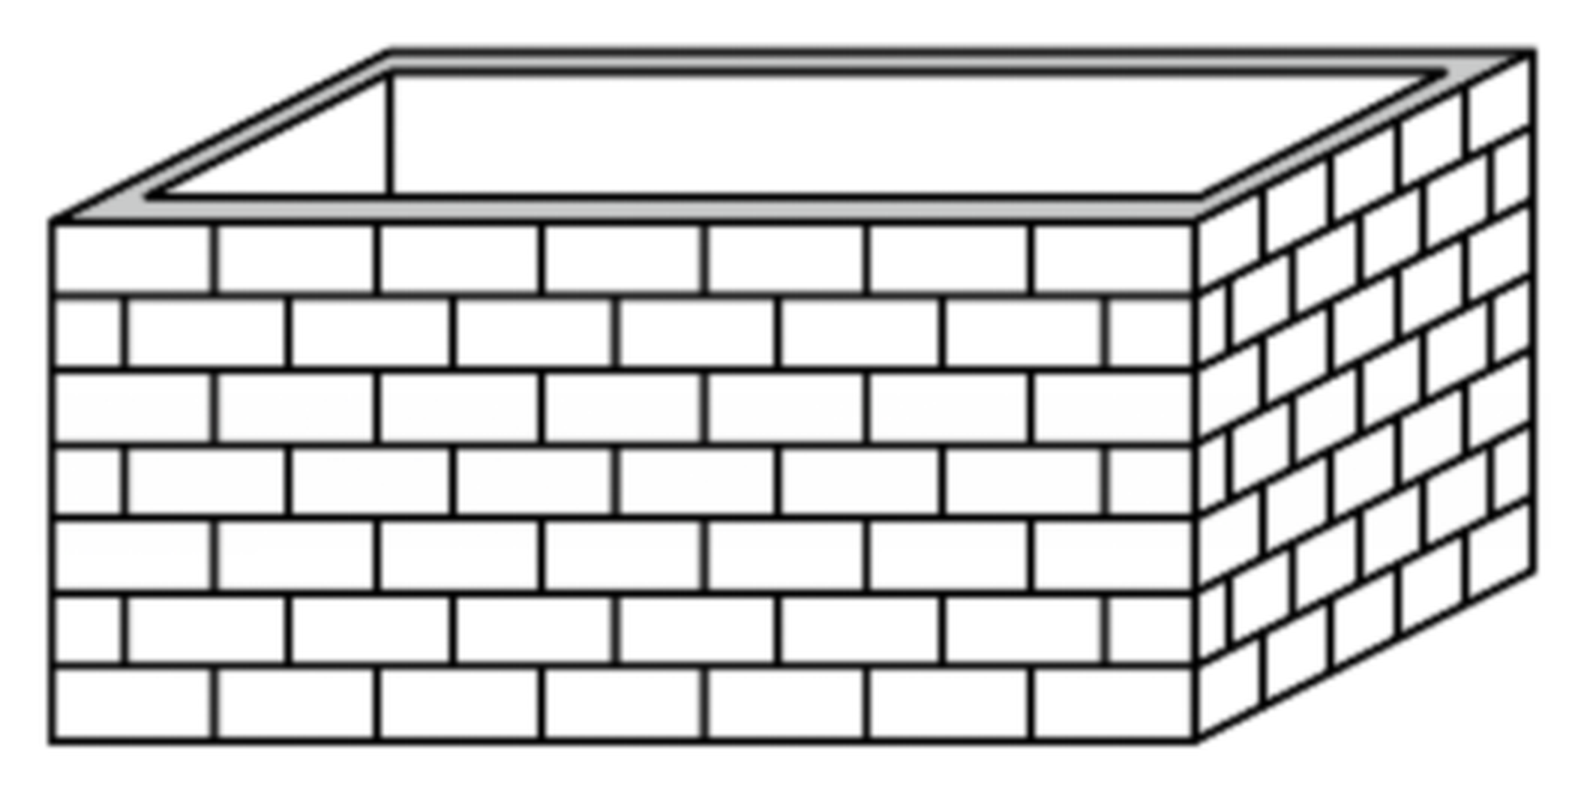
\includegraphics[width=0.42\textwidth]{figures/gao141_q19.png}
\end{center}

\ifanswer
\solbegin
\step{(1) 设水池的长、宽分别为 $xm$，$ym$，则 $x-y\geqslant60$，且 $x$、$y>0$，}
\step{由题意得 $2xy=3200$，即 $x=\dfrac{1600}{y}$，所以 $\dfrac{1600}{y}-y\geqslant60$，}
\step{因为 $y>0$，所以 $1600-y^2\geqslant60y$，}
\step{即 $y^2+60y-1600=(y+80)(y-20)\leqslant0$，解得 $-80\leqslant y\leqslant20$，}
\step{又 $y>0$，所以 $0<y\leqslant20$，所以水池的宽的最大值为 $20m$.}
\step{(2) 设水池总造价为 $z$ 元，}
\step{则 $z=1600\times150+2\times(2x+2y)\times120=240000+480(x+y)$，}
\step{又因为 $y=\dfrac{1600}{x}$，}
\step{所以 $z=240000+\left(x+\dfrac{1600}{x}\right)\times480\geqslant240000+480\times2\sqrt{1600}$}
\step{$=240000+38400=278400$，}
\step{当且仅当 $x=\dfrac{1600}{x}$，即 $x=y=40$ 时取等号，}
\step{所以，将水池的池底设计为边长为 $40m$ 的正方形时总造价最低，}
\step{最低总造价为 $278400$ 元.}
\solend
\fi

\item 已知 $a\in\R$，设集合 $A=\{x\mid ax^2-3x+2<ax-1\}$.

(1) 若 $A=(1,3)$，求实数 $a$ 的值；

(2) 当 $a>0$ 时，求 $A$；

(3) 若 “ $x\in\left(\dfrac12,+\infty\right)$ ” 是 “ $x\in A$ ” 的必要非充分条件，求实数 $a$ 的取值范围.

\ifanswer
\solbegin
\step{原不等式等价于 $ax^2-(a+3)x+3<0\Leftrightarrow(x-1)(ax-3)<0$，}
\step{(1) $A=(1,3)$ 为有界区间，因此 $a>0$，两根为 $1$ 和 $\dfrac3a$，于是 $\dfrac3a=3$，得 $a=1$；}
\step{此时 $(x-1)(x-3)<0$ 的解集确为 $(1,3)$.}
\step{(2) 当 $a>0$ 时，二次项系数为正，比较 $1$ 与 $\dfrac3a$，得 $A=\begin{cases}\left(1,\dfrac3a\right),&0<a<3\\\varnothing,&a=3\\\left(\dfrac3a,1\right),&a>3\end{cases}$，}
\step{其中 $a=3$ 时，原不等式为 $3(x-1)^2<0$，无解.}
\step{(3) 记 $S=\left(\dfrac12,+\infty\right)$，题意要求 $A\subset S$.}% 子集符号原卷印单线 $\subset$，照录
\step{由于对任意 $a$ 都有 $1\notin A$，而 $1\in S$，所以只需满足 $A\subseteq S$.}
\step{当 $a<0$ 时，$A=\left(-\infty,\dfrac3a\right)\cup(1,+\infty)$，含有小于 $\dfrac12$ 的数，不符合条件.}
\step{当 $a=0$ 时，$A=(1,+\infty)$，符合条件.}
\step{当 $0<a<3$ 时，$A=\left(1,\dfrac3a\right)\subseteq S$；}
\step{当 $a=3$ 时，$A=\varnothing\subseteq S$，均符合条件；}
\step{当 $a>3$ 时，$A=\left(\dfrac3a,1\right)$，所以 $A\subseteq S\Leftrightarrow\dfrac3a\geqslant\dfrac12\Leftrightarrow a\leqslant6$；}
\step{因此实数 $a$ 的取值范围为 $[0,6]$.}
\solend
\fi

\item 甲、乙两同学探讨了一个问题：已知正实数 $x,y$ 满足 $3x+y=1$，求 $\dfrac1x+\dfrac1y$ 的最小值.

甲给出的解法：由 $1=3x+y\geqslant2\sqrt{3xy}$，得 $\sqrt{xy}\leqslant\dfrac{\sqrt3}{6}$，所以 $\dfrac1x+\dfrac1y\geqslant2\sqrt{\dfrac1{xy}}\geqslant4\sqrt3$. 因此 $\dfrac1x+\dfrac1y$ 的最小值为 $4\sqrt3$.

乙给出的解法：$\dfrac1x+\dfrac1y=\left(\dfrac1x+\dfrac1y\right)(3x+y)=4+\dfrac yx+\dfrac{3x}{y}$，因为 $x,y$ 均为正实数，所以 $\dfrac1x+\dfrac1y\geqslant4+2\sqrt{\dfrac yx\cdot\dfrac{3x}{y}}=4+2\sqrt3$.

(1) 请判断上述哪位同学的解法正确，哪位同学的解法错误，并指出错误的原因；

(2) 结合上述探讨，试求当 $0<x<\dfrac12$ 时，$\dfrac1x+\dfrac1{1-2x}$ 的最小值以及此时实数 $x$ 的值；

(3) 已知 $x$ 为正实数，$y$ 为非负实数，且 $x+2y=2$，求 $\dfrac{x^2+1}{x}+\dfrac{2y^2}{y+1}$ 的最小值以及此时实数 $x,y$ 的值.

\ifanswer
\solbegin
\step{(1) 甲的推导中，$3x+y\geqslant2\sqrt{3xy}$ 取等号要求 $3x=y$，}
\step{$\dfrac1x+\dfrac1y\geqslant\dfrac2{\sqrt{xy}}$ 取等号要求 $x=y$，两者对正实数 $x,y$ 不能同时成立，}
\step{因此不能将 $4\sqrt3$ 判为最小值，甲错误.}
\step{乙的等号条件为 $\dfrac yx=\dfrac{3x}{y}$，即 $y=\sqrt3 x$；}
\step{结合 $3x+y=1$，得 $x=\dfrac1{3+\sqrt3},y=\dfrac{\sqrt3}{3+\sqrt3}$ 均为正数，等号可以成立，}
\step{因此乙正确，最小值为 $4+2\sqrt3$.}
\step{(2) 令 $t=1-2x>0$，则 $2x+t=1$.}
\step{$\dfrac1x+\dfrac1t=\left(\dfrac1x+\dfrac1t\right)(2x+t)=3+\dfrac tx+\dfrac{2x}{t}\geqslant3+2\sqrt2$，}
\step{当且仅当 $\dfrac tx=\dfrac{2x}{t}$，即 $t=\sqrt2 x$ 时取等号，}
\step{由 $2x+t=1$，得 $x=\dfrac1{2+\sqrt2}=\dfrac{2-\sqrt2}{2}\in\left(0,\dfrac12\right)$，}
\step{因此最小值为 $3+2\sqrt2$，此时 $x=\dfrac{2-\sqrt2}{2}$.}
\step{(3) 记目标式为 $F$，利用 $x+2y=2$，}
\step{得 $F=x+\dfrac1x+2y-2+\dfrac2{y+1}=\dfrac1x+\dfrac2{y+1}$，}
\step{又 $x+2(y+1)=4$，且 $x>0$、$y+1>0$，}
\step{所以 $4F=\left(\dfrac1x+\dfrac2{y+1}\right)(x+2(y+1))=5+2\left(\dfrac{y+1}{x}+\dfrac{x}{y+1}\right)$}
\step{$\geqslant5+2\times2=9$，当且仅当 $\dfrac{y+1}{x}=\dfrac{x}{y+1}$，即 $x=y+1$ 时取等号.}
\step{联立 $x+2y=2$，得 $x=\dfrac43$、$y=\dfrac13$，满足题设条件，}
\step{因此最小值为 $\dfrac94$，此时 $x=\dfrac43$，$y=\dfrac13$.}
\solend
\fi

\end{enumerate}

\end{document}
"
%
% ① 原始材料：微信公众号"魔都数学加油站"文章，连载"27学年高一141"，原文标题
% "27学年高一141——2026-2027年上海市彭浦中学高一上期中"；
% 原文链接：https://mp.weixin.qq.com/s/V_8bEhC6geeFyQysmtqUtQ。
% 正文为 9 张 PNG 页（01、05、06、07、09 为 2560x3620；02、03、04、08 为 4762x6735，
% 同一篇各页分辨率不同，逐页按各自分辨率放大裁图核对），题目下印【解析】，为讲评版。
% 题目、解析均据原图转录；卷面粉红色水印"魔都数学加油站"及公众号页脚未录入。
% 全卷 2 幅插图，均属题目配图（在 \ifanswer 外、三版都出）、取原卷截图去粉色水印、
% LANCZOS 放大 3 倍：第 5 题韦恩图（01 页，全集 U 矩形内两圆相交、交集阴影、A/B/U 标注）、
% 第 19 题长方体无盖贮水池砖墙示意图（06 页右上）。通读 9 页确认除这 2 幅外无其它
% 插图/表格，亦无"题干写如图而源码漏图"（仅 Q5"图中阴影部分"、Q19"如图所示"两处提到图）。
%
% 卷首标题：原卷印作"2026-2027 年彭浦中学高一上期中"（公众号标题中的"上海市"
% 卷面标题行没有，本稿照卷面），年份区间按全稿惯例排 en dash；原卷未印副标题，
% 本卷为期中卷、跨集合与常用逻辑用语／不等式／函数三章，按题目内容补出
% "集合与常用逻辑用语、不等式、函数"（与 高一140 同期中卷口径相同）：
% 集合与逻辑见 Q5、Q10、Q12、Q13、Q16、Q17、Q20，不等式见 Q4、Q9、Q14、Q18、
% Q19、Q21，函数（指数／对数）见 Q6、Q15。
%
% 题号体例：本卷共 19 题——一、填空题 3—12（10 题）、二、选择题 13—16（4 题）、
% 三、解答题 17—21（5 题）。三节分别 \setcounter{enumi}{2}／{12}／{16}。
% 原卷从第 3 题起、无第 1、2 题，本稿保留原题号；全卷无附加题节。
%
% ② 与原卷的排版差异：
%   ① 原文从第 3 题起，本稿保留原题号；
%   ② 原卷 19 题题下均印【解析】，无独立【答案】段、无"答案印题干括号且无解析"、
%      无"只印【答案】无解析"一型：填空题与解答题的答案落在【解析】末句
%      （Q3—Q12、Q17—Q21），四道选择题答案在【解析】末句"故选 …"
%      （Q13 选 A、Q14 选 C、Q15 选 D、Q16 选 C），题干括号内一律留空；
%      本稿 19 题一律 \solbegin…\solend、全卷不提 \ans{}，答案版【解析】标记数
%      = 19 = 全卷题数（无【答案】标记）；
%   ③ 原卷未印副标题，本稿按"知识模块"口径补出；
%   ④ 原卷填空横线按全稿惯例排 \blankline[4.4em]；选择题括号排 \mbox{（\quad）}，
%      选项段／命题段前按惯例加 \keepwithprev（Q16 两枚：命题列与选项段各一）；
%      解答题不留作答区、不加 \anspace（原卷为讲评版，与 129／131／132／133／136／140 同）；
%   ⑤ 原卷数集混排：黑板粗体 R（Q14 题干、Q16 ① 与解析、Q17 全集、Q20 题干）
%      按全稿惯例统一改 \R；空集记号 \varnothing；绝对值排 \lvert…\rvert，
%      集合描述竖线排 \mid；不等号按全稿惯例排 \leqslant／\geqslant；
%      补集照原卷上划线排 \overline{A\cap B}（Q17(2) 题干与解析）；
%      原卷"card"记号排黑体正体（Q12），本稿照录 \mathbf{card}，未改斜体
%      （与 高一66 同题口径不同：那份原卷 card 排斜体、照录 $card(M)$）；
%   ⑥ 子题标号 (1)(2)(3) 原卷印半角括号，照录；圈数字 ①②③④ 在正文（文本模式）
%      按原卷照录，未进数学式；数学式内半角逗号照录（如 Q12"$A,B$"、"{1,2,3}"、
%      Q14"$a,b,c\in\R$"、Q15"$\log_{14}7=a$，$14^b=5$"、Q16"$a=1,b=0$"、
%      Q18"$x,y,z$"、Q20"$x,y$"、Q21"$x,y$"）；全卷行末西文句点照录为 ASCII 句点；
%      行中全角逗号、顿号照录；
%   ⑦ 题干中的中文弯引号按原卷照录（Q13、Q20(3) 的 “ ” 及引号内空格），
%      注释内一律 ASCII 引号；
%   ⑧ 两幅题目配图各在 \item 之前加 \needvspace 守卫整块推走（Q5 5cm、Q19 6cm），
%      守卫放在 \item 之前而非 \bigsec 之后——两题均非各节首题，不触发 B 类
%      "节标题落页末"（照 高一26／40／59／136／140 成例）；三版切页审计均"合计异常：无"；
%   ⑨ 跨页续印按题合并：Q8 题干与【解析】首行在 01 页、后 6 行在 02 页；
%      Q15 题干在 03 页、【解析】在 04 页；Q17 题干与【解析】前 2 行在 04 页、
%      后 4 行在 05 页；Q19 题干在 05 页末、(1)(2) 小问与砖墙图与【解析】在 06 页；
%      Q20 题干 (1)(2) 在 06 页末、(3) 与【解析】在 07 页；Q21 题干与【解析】
%      前 6 行在 08 页、后 12 行在 09 页；Q16、Q18 全在各自页内；
%      本稿按题连排，不丢行；
%   ⑩ 原卷无红色加粗标签（【解析】均黑色印刷，Q16 解析 "①取…""④取…" 与
%      Q20 解析 "(2)" 等分步标签亦黑色），故本卷未用 \stepm；
%   ⑪ 原卷 Q19 题干把数值与单位（3200m³、2m、60m、150 元、120 元、40m、20m、
%      278400 元）印作略粗的西文字形，本稿按全稿惯例（高一70／72 同类题）排普通
%      数学体，未加粗。
%
% ③ 行数复核：一条 \step = 原卷解析的一个印刷行，cases 块作一个印刷行计。逐题数 \step
%   条数，合计 92 条（Q3：1；Q4：1；Q5：1；Q6：1；Q7：2；Q8：7；Q9：1；Q10：4；
%   Q11：4；Q12：4；Q13：2；Q14：1；Q15：2；Q16：4；Q17：6；Q18：7；Q19：13；
%   Q20：13；Q21：18），与原卷印刷行逐题相等。全卷 19 题均印【解析】、无独立 \ans{}，
%   答案版【解析】标记数 = 19 = 全卷题数。
%
% ④ 判别式／子集符号结论（逐处放大原图照录、不得统一）：
%   判别式：全卷 3 处——第 7 题【解析】"$\Delta=a^2-4\cdot\frac14=0$"一处原卷印
%     等腰、偏高的高三角 $\Delta$，照录 \Delta；第 8 题【解析】
%     "$\triangle=25-40=-15<0$"与"$\triangle=1+8=9>0$"两处原卷印扁等边三角
%     $\triangle$，照录 \triangle。两形不同，逐处照录未统一。
%   子集：全卷 6 处——第 10 题【解析】"$B\subseteq A$"一处、第 20 题【解析】
%     "所以只需满足 $A\subseteq S$"、"$A=\left(1,\frac3a\right)\subseteq S$"、
%     "$A=\varnothing\subseteq S$"、"$A\subseteq S\Leftrightarrow\frac3a\geqslant\frac12$"
%     四处，共 5 处原卷印带下划线的 $\subseteq$，照录 \subseteq；第 20 题【解析】
%     (3) 首行"题意要求 $A\subset S$"一处原卷印单线 $\subset$，照录 \subset
%     （下行因 $1\in S$ 而 $1\notin A$，改述为 $A\subseteq S$，两者逻辑一致、非笔误）。
%
% ⑤ 存疑照录（照录未改，正文对应处另有 % 注）：
%   第 14 题题干"设 $a,b,c\in\R$"只声明 $a,b,c$，而 A 选项"若 $a>b$ 且 $c>d$，
%     则 $ac>bd$"引入未声明的 $d$，原卷变量声明与选项不统一，照录未补。
%   全卷除此 1 条外未发现其它笔误／自相矛盾处。
%
% ⑥ 跨页续印按题合并说明：见 ② ⑨。
%
\documentclass[a4paper,11pt]{article}
\usepackage{common}

\begin{document}

\examtitlest[3]{2026--2027 年彭浦中学高一上期中}{集合与常用逻辑用语、不等式、函数}

\bigsec{一、填空题}

\begin{enumerate}
\setcounter{enumi}{2}

\item 已知 $m$ 为实数，若 $1\in\{m,m^2\}$，则 $m$ 的值为\blankline[4.4em].

\ifanswer
\solbegin
\step{$m=1$ 或 $m^2=1$，得 $m=\pm1$；按列举项互异口径排除 $m=m^2=1$，得 $m=-1$.}
\solend
\fi

\item 已知 $2<a<4$，$-2<b<1$，则 $2a+b$ 的取值范围为\blankline[4.4em].

\ifanswer
\solbegin
\step{$4<2a<8$，与 $-2<b<1$ 相加，得 $2<2a+b<9$，取值范围为 $(2,9)$.}
\solend
\fi

% 第 5 题韦恩图（题目配图，三版都出）：取原卷 01 页截图去粉色水印、LANCZOS 放大 3 倍
\needvspace{5cm}
\item 已知集合 $A=\{-1,-2,1,4,7\}$，$B=\{x\mid x>1\}$，用列举法表示图中阴影部分所表示的集合为\blankline[4.4em].

\begin{center}
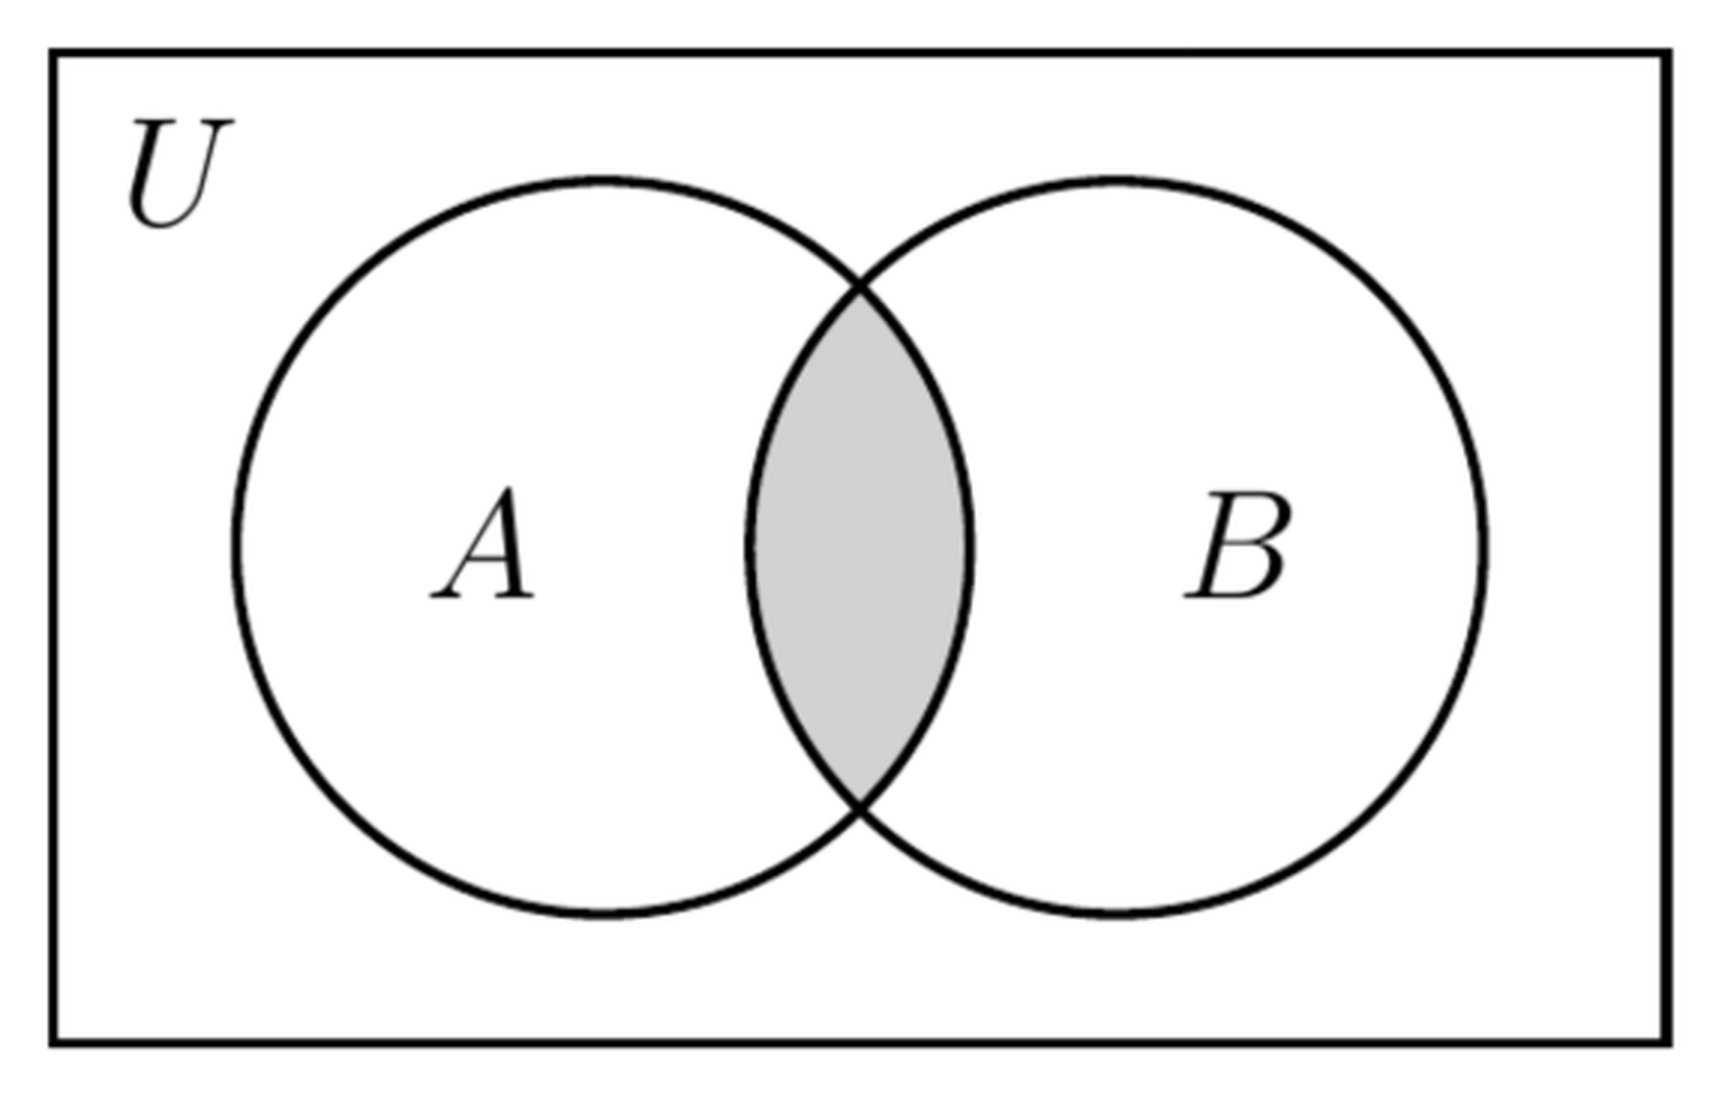
\includegraphics[width=0.38\textwidth]{figures/gao141_q5.png}
\end{center}

\ifanswer
\solbegin
\step{阴影部分表示 $A\cap B=\{4,7\}$.}
\solend
\fi

\item 方程 $2^{\log_3 x}=\dfrac12$ 的解集为\blankline[4.4em].

\ifanswer
\solbegin
\step{$2^{\log_3 x}=2^{-1}\Leftrightarrow\log_3 x=-1\Leftrightarrow x=\dfrac13$，解集为 $\left\{\dfrac13\right\}$.}
\solend
\fi

\item 若集合 $A=\left\{x\mid x^2+ax+\dfrac14=0\right\}$ 有且仅有两个子集，则实数 $a$ 的值为\blankline[4.4em].

\ifanswer
\solbegin
\step{$A$ 有且仅有两个子集，说明 $A$ 恰有一个元素，即方程有两个相等的实数根.}
\step{$\Delta=a^2-4\cdot\dfrac14=0\Rightarrow a=\pm1$.}% 判别式原卷印等腰偏高的高三角 $\Delta$，照录
\solend
\fi

\item 已知关于 $x$ 的方程 $x^2+mx+2m=0$ 的两个实数根分别为 $\alpha$、$\beta$，若 $\alpha^2+\beta^2=5$，则实数 $m=$\blankline[4.4em].

\ifanswer
\solbegin
\step{方程 $x^2+mx+2m=0$ 的两个实数根为 $\alpha$、$\beta$，}
\step{由根与系数的关系得 $\begin{cases}\alpha+\beta=-m\\\alpha\beta=2m\end{cases}$，又因为 $\alpha^2+\beta^2=5$，}
\step{所以 $\alpha^2+\beta^2=(\alpha+\beta)^2-2\alpha\beta=m^2-4m=5$，整理得 $m^2-4m-5=0$，}
\step{解得 $m=5$ 或 $m=-1$，}
\step{当 $m=5$ 时，$\triangle=25-40=-15<0$，无实根，舍去；}% 判别式原卷印扁等边三角 $\triangle$，照录
\step{当 $m=-1$ 时，$\triangle=1+8=9>0$，符合题意，}
\step{所以实数 $m=-1$.}
\solend
\fi

\item 若不等式 $\lvert x-3\rvert+\lvert x-5\rvert\geqslant a$ 对任意的实数 $x$ 恒成立，则实数 $a$ 的取值范围为\blankline[4.4em].

\ifanswer
\solbegin
\step{由三角不等式得 $\lvert x-3\rvert+\lvert x-5\rvert\geqslant\lvert x-3-x+5\rvert=2$，则 $a\leqslant2$.}
\solend
\fi

\item 设集合 $A=\{-3,2\}$，集合 $B=\{x\mid mx+1=0\}$，若 $A\cup B=A$，则实数 $m$ 的值为\blankline[4.4em].

\ifanswer
\solbegin
\step{由 $A\cup B=A$，得 $B\subseteq A$，}% 子集符号原卷印带下划线的 $\subseteq$，照录
\step{当 $m=0$ 时，$B=\varnothing$，满足题意，}
\step{当 $m\neq0$ 时，$B=\left\{-\dfrac1m\right\}$，所以 $-\dfrac1m=2$ 或 $-\dfrac1m=-3$，所以 $m=-\dfrac12$ 或 $m=\dfrac13$，}
\step{综上所述，$m=0$ 或 $m=-\dfrac12$ 或 $m=\dfrac13$.}
\solend
\fi

\item 已知 $m$ 为实数，代数式 $M=\sqrt{m-1}+\sqrt{3-m}$ 的取值范围为\blankline[4.4em].

\ifanswer
\solbegin
\step{根式有意义要求 $m\in[1,3]$，}
\step{此时 $(m-1)(3-m)=1-(m-2)^2$ 的取值范围为 $[0,1]$.}
\step{$M^2=2+2\sqrt{(m-1)(3-m)}$ 的取值范围为 $[2,4]$，又 $M>0$，}
\step{所以 $M\in[\sqrt2,2]$.}
\solend
\fi

\item 设有限集 $M$ 所含元素的个数用 $\mathbf{card}(M)$ 表示，并规定 $\mathbf{card}(\varnothing)=0$. 已知集合 $A,B$ 满足 $A\cup B=\{1,2,3\}$，$A\cap B=\varnothing$，若 $\mathbf{card}(A)\notin A$，$\mathbf{card}(B)\notin B$，则满足条件的所有不同集合 $A$ 的个数为\blankline[4.4em].

\ifanswer
\solbegin
\step{当 $\mathbf{card}(A)=0$ 或 $3$ 时，$A,B$ 中有一个为 $\{1,2,3\}$，不符合条件.}
\step{当 $\mathbf{card}(A)=1$ 时，$\mathbf{card}(B)=2\notin B$，所以 $A=\{2\}$，符合条件.}
\step{当 $\mathbf{card}(A)=2$ 时，$2\notin A$，所以 $B=\{2\}$，$A=\{1,3\}$，符合条件.}
\step{满足条件的集合 $A$ 共 $2$ 个.}
\solend
\fi

\end{enumerate}

\bigsec{二、选择题}

\begin{enumerate}
\setcounter{enumi}{12}

\item “ $x=1$ ” 是 “ $x^2-3x+2=0$ ” 的\mbox{（\quad）}条件.

\keepwithprev
A. 充分非必要\qquad B. 必要非充分

C. 充要\qquad D. 既非充分又非必要

\ifanswer
\solbegin
\step{$x^2-3x+2=0\Leftrightarrow x=1$ 或 $x=2$，所以 “ $x=1$ ” 是其充分非必要条件，}
\step{故选 $A$.}
\solend
\fi

\item 设 $a,b,c\in\R$，则下列命题为真命题的是\mbox{（\quad）}
% 原卷题干只声明 a,b,c，而 A 选项出现未声明的 d，照录（存疑）
\keepwithprev
A. 若 $a>b$ 且 $c>d$，则 $ac>bd$\qquad B. 若 $a^2>b^2$，则 $a>b$

C. 若 $ab>0$ 且 $a>b$，则 $\dfrac1a<\dfrac1b$\qquad D. 若 $a<0<b$，则 $\sqrt{-a}<\sqrt b$

\ifanswer
\solbegin
\step{$ab>0$ 且 $a>b\Rightarrow\dfrac1a-\dfrac1b=\dfrac{b-a}{ab}<0$，所以 $C$ 为真命题，故选 $C$.}
\solend
\fi

\item 已知 $\log_{14}7=a$，$14^b=5$，则 $\log_{35}28=$\mbox{（\quad）}

\keepwithprev
A. $\dfrac{2-a}{2a+b}$\qquad B. $\dfrac{2+a}{a+b}$\qquad C. $\dfrac{2-a}{a+2b}$\qquad D. $\dfrac{2-a}{a+b}$

\ifanswer
\solbegin
\step{$\log_{14}7=a$，$14^b=5$，}
\step{$\log_{35}28=\dfrac{\log_{14}28}{\log_{14}35}=\dfrac{\log_{14}14^2-\log_{14}7}{\log_{14}7+\log_{14}5}=\dfrac{2-a}{a+b}$. 故选 $D$.}
\solend
\fi

\item 关于 $x$ 的不等式 $ax^2+bx+3>0$ 的解集有下列说法，其中正确的个数是\mbox{（\quad）}

\keepwithprev
① 不等式 $ax^2+bx+3>0$ 的解集可以是 $\R$

② 不等式 $ax^2+bx+3>0$ 的解集可以是 $\{x\mid x>3\}$

③ 不等式 $ax^2+bx+3>0$ 的解集可以是 $\varnothing$

④ 不等式 $ax^2+bx+3>0$ 的解集可以是 $\{x\mid -1<x<3\}$

\keepwithprev
A. 4\qquad B. 3\qquad C. 2\qquad D. 1

\ifanswer
\solbegin
\step{$x=0$ 时左端为 $3>0$，解集必含 $0$，所以②③错误.}
\step{①取 $a=1,b=0$，$x^2+3>0$ 的解集为 $\R$，正确.}
\step{④取 $a=-1,b=2$，$-x^2+2x+3=-(x+1)(x-3)>0\Leftrightarrow-1<x<3$，正确.}
\step{正确的有①④，共 $2$ 个，故选 $C$.}
\solend
\fi

\end{enumerate}

\bigsec{三、解答题}

\begin{enumerate}
\setcounter{enumi}{16}

\item 已知集合 $A=\left\{x\mid\dfrac{x-2}{x+3}\geqslant0\right\}$，集合 $B=\{x\mid\lvert x+1\rvert+\lvert x-1\rvert<5\}$，全集 $U=\R$.

(1) 求 $A,B$；

(2) 求 $A\cup B$、$\overline{A\cap B}$.

\ifanswer
\solbegin
\step{(1) 分母不为零，且分子、分母同号或分子为零，}
\step{所以 $\dfrac{x-2}{x+3}\geqslant0\Leftrightarrow x<-3$ 或 $x\geqslant2$，因此 $A=(-\infty,-3)\cup[2,+\infty)$.}
\step{又 $\lvert x+1\rvert+\lvert x-1\rvert=\begin{cases}-2x,&x<-1\\2,&-1\leqslant x\leqslant1\\2x,&x>1\end{cases}$，}
\step{分别解得 $-\dfrac52<x<-1$、$-1\leqslant x\leqslant1$、$1<x<\dfrac52$，因此 $B=\left(-\dfrac52,\dfrac52\right)$.}
\step{(2) 合并两集合所对应的区间，得 $A\cup B=(-\infty,-3)\cup\left(-\dfrac52,+\infty\right)$，}
\step{两集合的公共部分为 $A\cap B=\left[2,\dfrac52\right)$，所以 $\overline{A\cap B}=(-\infty,2)\cup\left[\dfrac52,+\infty\right)$.}
\solend
\fi

\item (1) 已知 $a>b>0$，比较代数式 $\dfrac ab$ 与 $\dfrac{a+1}{b+1}$ 的大小并说明理由；

(2) 已知 $x,y,z$ 都是正实数，$a=x+\dfrac1y,b=y+\dfrac1z,c=z+\dfrac1x$，试用反证法证明 $a,b,c$ 至少有一个不小于 $2$.

\ifanswer
\solbegin
\step{(1) $\dfrac ab-\dfrac{a+1}{b+1}=\dfrac{a(b+1)-b(a+1)}{b(b+1)}=\dfrac{a-b}{b(b+1)}$，}
\step{因为 $a>b>0$，所以 $a-b>0$，$b(b+1)>0$，所以 $\dfrac ab-\dfrac{a+1}{b+1}>0$，}
\step{故 $\dfrac ab>\dfrac{a+1}{b+1}$.}
\step{(2) 假设 $a$、$b$、$c$ 三数都小于 $2$，则 $x+\dfrac1y+y+\dfrac1z+z+\dfrac1x<6$.}
\step{因为 $x,y,z$ 均大于 $0$，}
\step{所以 $x+\dfrac1y+y+\dfrac1z+z+\dfrac1x=x+\dfrac1x+y+\dfrac1y+z+\dfrac1z\geqslant2+2+2=6$，矛盾，}
\step{所以 $a$、$b$、$c$ 三数中至少有一个不小于 $2$.}
\solend
\fi

% 第 19 题长方体无盖贮水池砖墙示意图（题目配图，三版都出）：取原卷 06 页截图去粉色水印、LANCZOS 放大 3 倍
\needvspace{6cm}
\item 如图所示，某工厂要建造一个长方体形无盖贮水池，其容积为 $3200m^3$，深为 $2m$.

(1) 若水池的长比宽至少多 $60m$，求水池的宽的最大值；

(2) 若池底每平方米的造价为 $150$ 元，池壁每平方米的造价为 $120$ 元，那么怎样设计水池的长和宽能使总造价最低？最低总造价是多少？

\begin{center}
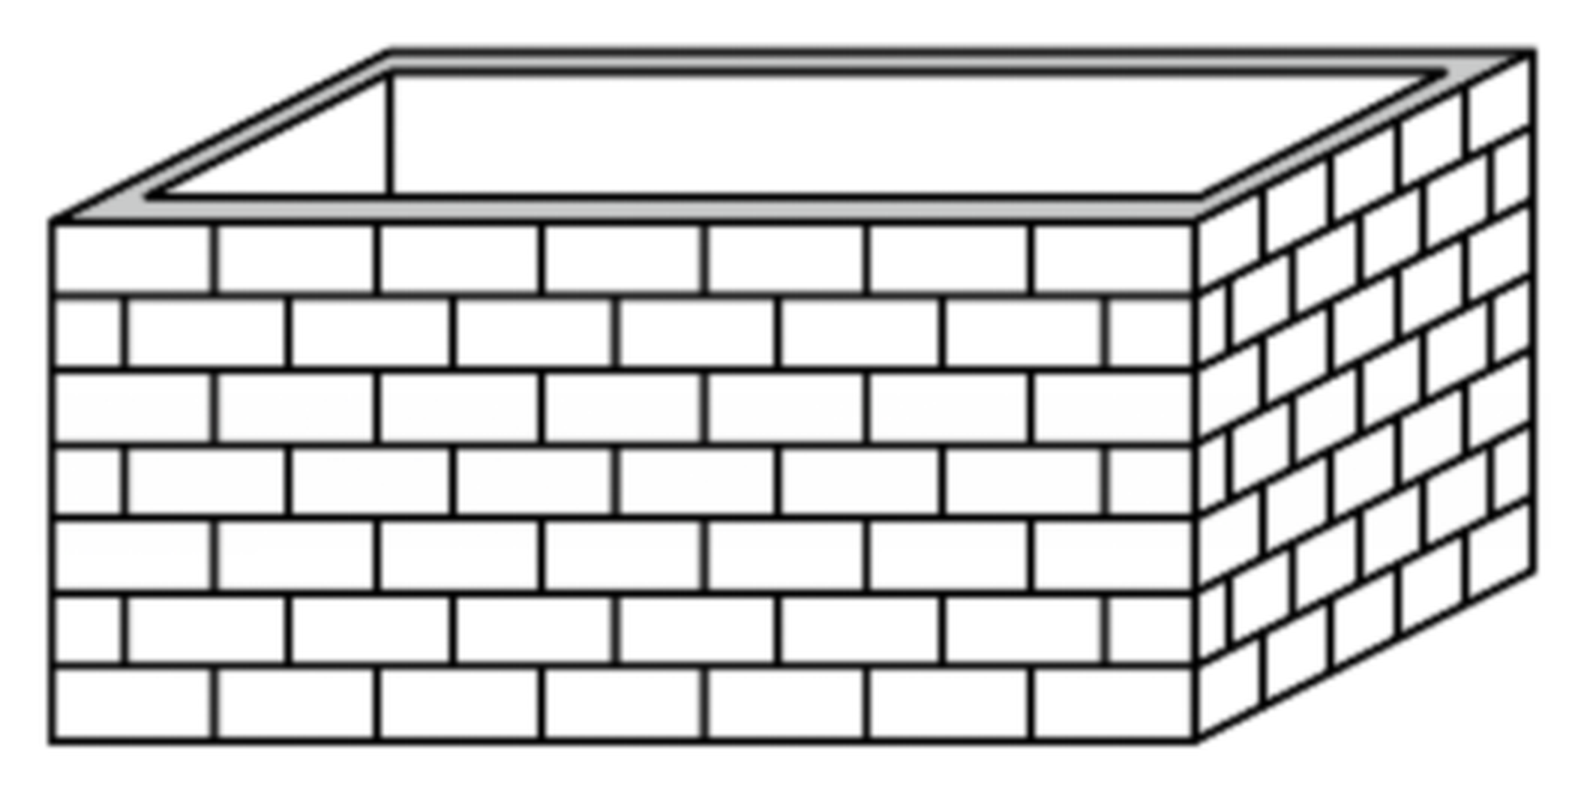
\includegraphics[width=0.42\textwidth]{figures/gao141_q19.png}
\end{center}

\ifanswer
\solbegin
\step{(1) 设水池的长、宽分别为 $xm$，$ym$，则 $x-y\geqslant60$，且 $x$、$y>0$，}
\step{由题意得 $2xy=3200$，即 $x=\dfrac{1600}{y}$，所以 $\dfrac{1600}{y}-y\geqslant60$，}
\step{因为 $y>0$，所以 $1600-y^2\geqslant60y$，}
\step{即 $y^2+60y-1600=(y+80)(y-20)\leqslant0$，解得 $-80\leqslant y\leqslant20$，}
\step{又 $y>0$，所以 $0<y\leqslant20$，所以水池的宽的最大值为 $20m$.}
\step{(2) 设水池总造价为 $z$ 元，}
\step{则 $z=1600\times150+2\times(2x+2y)\times120=240000+480(x+y)$，}
\step{又因为 $y=\dfrac{1600}{x}$，}
\step{所以 $z=240000+\left(x+\dfrac{1600}{x}\right)\times480\geqslant240000+480\times2\sqrt{1600}$}
\step{$=240000+38400=278400$，}
\step{当且仅当 $x=\dfrac{1600}{x}$，即 $x=y=40$ 时取等号，}
\step{所以，将水池的池底设计为边长为 $40m$ 的正方形时总造价最低，}
\step{最低总造价为 $278400$ 元.}
\solend
\fi

\item 已知 $a\in\R$，设集合 $A=\{x\mid ax^2-3x+2<ax-1\}$.

(1) 若 $A=(1,3)$，求实数 $a$ 的值；

(2) 当 $a>0$ 时，求 $A$；

(3) 若 “ $x\in\left(\dfrac12,+\infty\right)$ ” 是 “ $x\in A$ ” 的必要非充分条件，求实数 $a$ 的取值范围.

\ifanswer
\solbegin
\step{原不等式等价于 $ax^2-(a+3)x+3<0\Leftrightarrow(x-1)(ax-3)<0$，}
\step{(1) $A=(1,3)$ 为有界区间，因此 $a>0$，两根为 $1$ 和 $\dfrac3a$，于是 $\dfrac3a=3$，得 $a=1$；}
\step{此时 $(x-1)(x-3)<0$ 的解集确为 $(1,3)$.}
\step{(2) 当 $a>0$ 时，二次项系数为正，比较 $1$ 与 $\dfrac3a$，得 $A=\begin{cases}\left(1,\dfrac3a\right),&0<a<3\\\varnothing,&a=3\\\left(\dfrac3a,1\right),&a>3\end{cases}$，}
\step{其中 $a=3$ 时，原不等式为 $3(x-1)^2<0$，无解.}
\step{(3) 记 $S=\left(\dfrac12,+\infty\right)$，题意要求 $A\subset S$.}% 子集符号原卷印单线 $\subset$，照录
\step{由于对任意 $a$ 都有 $1\notin A$，而 $1\in S$，所以只需满足 $A\subseteq S$.}
\step{当 $a<0$ 时，$A=\left(-\infty,\dfrac3a\right)\cup(1,+\infty)$，含有小于 $\dfrac12$ 的数，不符合条件.}
\step{当 $a=0$ 时，$A=(1,+\infty)$，符合条件.}
\step{当 $0<a<3$ 时，$A=\left(1,\dfrac3a\right)\subseteq S$；}
\step{当 $a=3$ 时，$A=\varnothing\subseteq S$，均符合条件；}
\step{当 $a>3$ 时，$A=\left(\dfrac3a,1\right)$，所以 $A\subseteq S\Leftrightarrow\dfrac3a\geqslant\dfrac12\Leftrightarrow a\leqslant6$；}
\step{因此实数 $a$ 的取值范围为 $[0,6]$.}
\solend
\fi

\item 甲、乙两同学探讨了一个问题：已知正实数 $x,y$ 满足 $3x+y=1$，求 $\dfrac1x+\dfrac1y$ 的最小值.

甲给出的解法：由 $1=3x+y\geqslant2\sqrt{3xy}$，得 $\sqrt{xy}\leqslant\dfrac{\sqrt3}{6}$，所以 $\dfrac1x+\dfrac1y\geqslant2\sqrt{\dfrac1{xy}}\geqslant4\sqrt3$. 因此 $\dfrac1x+\dfrac1y$ 的最小值为 $4\sqrt3$.

乙给出的解法：$\dfrac1x+\dfrac1y=\left(\dfrac1x+\dfrac1y\right)(3x+y)=4+\dfrac yx+\dfrac{3x}{y}$，因为 $x,y$ 均为正实数，所以 $\dfrac1x+\dfrac1y\geqslant4+2\sqrt{\dfrac yx\cdot\dfrac{3x}{y}}=4+2\sqrt3$.

(1) 请判断上述哪位同学的解法正确，哪位同学的解法错误，并指出错误的原因；

(2) 结合上述探讨，试求当 $0<x<\dfrac12$ 时，$\dfrac1x+\dfrac1{1-2x}$ 的最小值以及此时实数 $x$ 的值；

(3) 已知 $x$ 为正实数，$y$ 为非负实数，且 $x+2y=2$，求 $\dfrac{x^2+1}{x}+\dfrac{2y^2}{y+1}$ 的最小值以及此时实数 $x,y$ 的值.

\ifanswer
\solbegin
\step{(1) 甲的推导中，$3x+y\geqslant2\sqrt{3xy}$ 取等号要求 $3x=y$，}
\step{$\dfrac1x+\dfrac1y\geqslant\dfrac2{\sqrt{xy}}$ 取等号要求 $x=y$，两者对正实数 $x,y$ 不能同时成立，}
\step{因此不能将 $4\sqrt3$ 判为最小值，甲错误.}
\step{乙的等号条件为 $\dfrac yx=\dfrac{3x}{y}$，即 $y=\sqrt3 x$；}
\step{结合 $3x+y=1$，得 $x=\dfrac1{3+\sqrt3},y=\dfrac{\sqrt3}{3+\sqrt3}$ 均为正数，等号可以成立，}
\step{因此乙正确，最小值为 $4+2\sqrt3$.}
\step{(2) 令 $t=1-2x>0$，则 $2x+t=1$.}
\step{$\dfrac1x+\dfrac1t=\left(\dfrac1x+\dfrac1t\right)(2x+t)=3+\dfrac tx+\dfrac{2x}{t}\geqslant3+2\sqrt2$，}
\step{当且仅当 $\dfrac tx=\dfrac{2x}{t}$，即 $t=\sqrt2 x$ 时取等号，}
\step{由 $2x+t=1$，得 $x=\dfrac1{2+\sqrt2}=\dfrac{2-\sqrt2}{2}\in\left(0,\dfrac12\right)$，}
\step{因此最小值为 $3+2\sqrt2$，此时 $x=\dfrac{2-\sqrt2}{2}$.}
\step{(3) 记目标式为 $F$，利用 $x+2y=2$，}
\step{得 $F=x+\dfrac1x+2y-2+\dfrac2{y+1}=\dfrac1x+\dfrac2{y+1}$，}
\step{又 $x+2(y+1)=4$，且 $x>0$、$y+1>0$，}
\step{所以 $4F=\left(\dfrac1x+\dfrac2{y+1}\right)(x+2(y+1))=5+2\left(\dfrac{y+1}{x}+\dfrac{x}{y+1}\right)$}
\step{$\geqslant5+2\times2=9$，当且仅当 $\dfrac{y+1}{x}=\dfrac{x}{y+1}$，即 $x=y+1$ 时取等号.}
\step{联立 $x+2y=2$，得 $x=\dfrac43$、$y=\dfrac13$，满足题设条件，}
\step{因此最小值为 $\dfrac94$，此时 $x=\dfrac43$，$y=\dfrac13$.}
\solend
\fi

\end{enumerate}

\end{document}
